%%%%%%%%%%%%%%%%%%%%%%%%%%%%%%%%%%%%%%%%%%%%%%%%%%%%%%%%%%
%%
%%                  Disserta��o de mestrado de
%%
%%                      F�bio Pisaruk
%%
%%
%%%%%%%%%%%%%%%%%%%%%%%%%%%%%%%%%%%%%%%%%%%%%%%%%%%%%%%%%%
\renewcommand{\P}{} % tira os Ps inc�modos

\documentclass[12pt,twoside]{book}


%\documentclass[language=brazil,structure=hiearchic,12pt]{book}

%% Colocando identa��o no primeiro par�grafo de cada t�pico
\usepackage{indentfirst}
%% Escrevendo em portugu�s:
\usepackage[brazil]{babel}
\usepackage[T1]{fontenc}
\usepackage[latin1]{inputenc}

%%%%%%%%%%%%%%%%%%%%%%%%%%%%%%%%%%%%%%%%%%%%%%%%%%%%%%%%%%%%%%%%%%%%%%
%% packages

\usepackage[dvips]{graphicx,psfrag}
\usepackage{palatino}
\usepackage{mathpazo}
\usepackage{multicol}
\usepackage{ifthen}
\usepackage{makeidx}
\usepackage{enumerate}
%\usepackage{fancyheadings}
\usepackage{fancyhdr}
\usepackage{multicol}
%% definicao personalizada
\usepackage{./estilo/estilo}
\usepackage{wrapfig}
\usepackage{sidecap}
\usepackage{listings} 
\usepackage{subfigure}	


%%%%%%%%%%%%%%%%%%%%%%%%%%%%%%%%%%%%%%%%%%%%%%%%%%%%%%%%%%%%%%%%%%%%%%
%% Floating package
\usepackage{floatflt}

%%%%%%%%%%%%%%%%%%%%%%%%%%%%%%%%%%%%%%%%%%%%%%%%%%%%%%%%%%%%%%%%%%%%%%

%%%%%%%%%%%%%%%%%%%%%%%%%%%%%%%%%%%%%%%%%%%%%%%%%%%%%%%%%%%
%% Dimens�o da p�gina
\setlength{\parskip}{.5pc}
\setlength{\paperwidth}{216mm}
\setlength{\paperheight}{279mm}
\setlength{\textwidth}{38pc}
\setlength{\textheight}{52pc}
\setlength{\topmargin}{0cm}

% margens impar e par da pagina
\setlength\oddsidemargin{.2cm}
\setlength\evensidemargin{.2cm}

%\setlength\oddsidemargin{.6cm}
%\setlength\evensidemargin{-.5cm}

\linespread{1.2}

% Fontes menores nos captions (para figuras e tabelas)
\newcommand{\captionfonts}{\small}

\makeatletter
\makeatother
\setcounter{tocdepth}{2}
\includeonly{
capa, 
agradecimentos,
01-resumo, 
abstract,
02-introducao, 
03-preliminares,
04-caminhos-minimos,
05-k-caminhos,
%06-yen,
07-kim,
08-resultados,
09-final,
05-katoh,
2.7-Dijkstra}

%\includeonly{capa, 08-facilitylocation}

\makeindex

% Aqui come�a o documento
\begin{document}

%\normalsize
%%%%%%%%%%%%%%%%%%%%%%%%%%%%%%%%%%%%%%%%%%%%%%%%%%%%%%%%%%%%%%%%%%%%%
%%
%%    CAPA
%%
%%%%%%%%%%%%%%%%%%%%%%%%%%%%%%%%%%%%%%%%%%%%%%%%%%%%%%%%%%%%%%%%%%%%%%
\thispagestyle{empty}
\vspace*{3cm}

\Large
\centerline{\bf Algoritmos para caminhos m�nimos} 
\vspace*{1cm}
\centerline{Shigueo Isotani}

\vspace*{2cm}

{\large \sc
\centerline{Disserta��o apresentada ao}
\centerline{Instituto de Matem�tica e }
\centerline{Estat�stica da}
\centerline{Universidade de S�o Paulo}
\centerline{como parte dos requisitos}
\centerline{para obten��o do grau de}
\centerline{Mestre em Ci�ncia da Computa��o}
}

\large
\vspace{2.0cm}
\centerline{Orientador: Prof. Dr. Jos� Coelho de Pina Jr.}

\normalsize
\vspace{1.0cm}
\centerline{--- S�o Paulo, mar�o de 2002\date{S�o Paulo, \today} ---}
%\date{S�o Paulo, \today}
\vspace{3.0cm}
\centerline{-- Durante o desenvolvimento deste trabalho, o aluno recebeu
apoio financeiro da CAPES --}


%\vspace*{3cm}

%\large
%\centerline{\bf Algoritmos para Caminhos M�nimos} 
%\vspace*{1cm}
%\centerline{Shigueo Isotani}

%\vspace*{2cm}

%{\large \sc
%\centerline{Disserta��o apresentada ao}
%\centerline{Instituto de Matem�tica e }
%\centerline{Estat�stica da}
%\centerline{Universidade de S�o Paulo}
%\centerline{como parte dos requisitos}
%\centerline{para obten��o do grau de}
%\centerline{Mestre em Ci�ncia da Computa��o}
%}

%\vspace{2.0cm}
%\centerline{Orientador: Prof. Dr. Jos� Coelho de Pina Jr.}

%\normalsize
%\vspace{1.0cm}
%\centerline{--- S�o Paulo, fevereiro de 2001\date{S�o Paulo, \today} ---}
%\date{S�o Paulo, \today}
%\vspace{3.0cm}
%\centerline{-- Durante o desenvolvimento deste trabalho, o aluno recebeu
%apoio financeiro da CAPES --}

%\clearemptydoublepage

\newpage

%%%%%%%%%%%%%%%%%%%%%%%%%%%%%%%%%%%%%%%%%%%%%%%%%%%%%%%%%%%%%%%%%%%%%%
%%
%%    BANCA
%%
%%%%%%%%%%%%%%%%%%%%%%%%%%%%%%%%%%%%%%%%%%%%%%%%%%%%%%%%%%%%%%%%%%%%%%

%%\thispagestyle{empty}
%%\vspace*{3cm}

\Large
\centerline{\bf Algoritmos para caminhos m�nimos} 
\vspace*{2cm}

{\large
\begin{flushright}
 Este exemplar corresponde � reda��o final \\
da  disserta��o devidamente corrigida e \\
defendida por Shigueo Isotani \\
e aprovada pela comiss�o  julgadora.\\
\vspace*{2cm}
S�o Paulo, 21 de mar�o de 2002\date{S�o Paulo, \today}
\end{flushright}
}

\vspace*{3cm}
{\large
Banca examinadora:
\begin{itemize}
\item Profa. Dra. Cristina Gomes Fernandes - IME-USP
\item Prof. Dr. Jos� Coelho de Pina Jr - IME-USP
\item Prof. Dr. Marcelo Henriques de Carvalho - DCT-UFMS
\end{itemize}
}
\normalsize
%%\newpage

%%%%%%%%%%%%%%%%%%%%%%%%%%%%%%%%%%%%%%%%%%%%%%%%%%%%%%%%%%%%%%%%%%%%%%
%%
%%    DEDICAT�RIA
%%
%%%%%%%%%%%%%%%%%%%%%%%%%%%%%%%%%%%%%%%%%%%%%%%%%%%%%%%%%%%%%%%%%%%%%%

\newpage
\thispagestyle{empty}
\vspace*{19cm}
\begin{flushright}
Aos meus pais Paulo e Roseli \\
e meu irm�o Marcos.
\end{flushright}


\newpage
\pagestyle{plain}
\pagenumbering{roman}
\setcounter{page}{1} 

%%%%%%%%%%%%%%%%%%%%%%%%%%%%%%%%%%%%%%%%%%%%%%%%%%%%%%%%%%%%%%%%%%%%%%
%%
%%    AGRADECIMENTOS
%%
%%%%%%%%%%%%%%%%%%%%%%%%%%%%%%%%%%%%%%%%%%%%%%%%%%%%%%%%%%%%%%%%%%%%%%
\newpage

\centerline{\Large{\textbf{Agradecimentos}}}
\addcontentsline{toc}{section}{Agradecimentos}

\vspace{0.3cm}

 Meus sinceros agradecimentos ao professor {\it Jos� Coelho}, pela forma
 dedicada e paciente com que me orientou. Esteve sempre presente e
 pronto a ajudar.
  
 Agrade�o ao {\it Rozante} e ao professor {\it Jos� Augusto} pelas valiosas dicas
 em rela��o ao uso do \CWEB{}, pois sem elas, ainda estaria tentando
 compilar esta disserta��o.

 Aos meus pais, {\it Sadao} e {\it Naoko}, pela demonstra��o de
 confian�a e carinho.  

 Aos meus irm�os, {\it Seiji} e {\it Mina}, pelo incentivo e pela ajuda com os
 deveres de casa, durante o per�odo da reda��o desta disserta��o.
 
 � minha namorada {\it Regina}.
 
 � Ana L�cia pela ajuda na prepara��o dos slides da apresenta��o.

 � CAPES pelo apoio financeiro proporcionado durante o desenvolvimento
desta disserta��o.

 Aos meus amigos {\it Exec}, {\it Inoue}, {\it Kubo}, {\it Lu�s Yano}, {\it Marcelo
 Vinagreiro}, {\it Noma} e {\it Wagner Dias} pela excelente
 companhia que me proporcionaram todos esses anos.


\newpage
\newpage
%%%%%%%%%%%%%%%%%%%%%%%%%%%%%%%%%%%%%%%%%%%%%%%%%%%%%%%%%%%%%%%%%%%%%%
%%
%%    RESUMO E ABSTRACT
%%
%%%%%%%%%%%%%%%%%%%%%%%%%%%%%%%%%%%%%%%%%%%%%%%%%%%%%%%%%%%%%%%%%%%%%%
%\thispagestyle{empty}
%\pagenumbering{arabic}
%\setcounter{page}{1}
%\pagestyle{empty}
\addcontentsline{toc}{section}{Resumo}
%\longpage

\centerline{\bf Resumo}

\vspace{0.4cm}

\noindent
Tratamos da generaliza��o do problema da gera��o de caminho m�nimo, 
no qual n�o apenas um, mas v�rios caminhos de menores custos devem ser produzidos.
O problema dos $k$-menores caminhos consiste em listar os $k$-caminhos de menores custos 
conectando um par de v�rtices.

Esta disserta��o trata de algoritmos para gera��o de $k$-menores caminhos em grafos sim�tricos 
com custos n�o-negativos, bem como algumas implementa��es destes.
 
 
\noindent \textbf{Palavras-chave:} caminhos m�nimos, k-menores caminhos.
 
%\vspace{2.0cm}

%\centerline{\bf Abstract} \vspace{0.4cm}

%\noindent
%We consider a long-studied generalization of the shortest path problem,
%in which not one but several short paths must be produced.
%The $k$-shortest (simple) paths problem is to list the $k$ paths 
%connecting a given source-destination pair in the digraph with minimum total length.

%This dissertation deals with $k$-shortest simple paths algorithms 
%designed for non-negative costs, undirected graphs and 
%some implementations of them. 





\newpage
\newpage
%\pagestyle{empty}
%%\addcontentsline{toc}{chapter}{Abstract}
%\longpage

\centerline{\bf Abstract}

\vspace{0.4cm}

\noindent
%%\chapter*{Abstract}

We consider a long-studied generalization of the shortest path problem,
in which not one but several short paths must be produced.
The $k$-shortest (simple) paths problem is to list the $k$ paths 
connecting a given source-destination pair in the digraph with minimum total length.

This dissertation deals with $k$-shortest simple paths algorithms 
designed for non-negative costs, undirected graphs and 
some implementations of them.

\noindent \textbf{Keywords:} shortest paths, $k$-shortest paths.

\newpage
%%%%%%%%%%%%%%%%%%%%%%%%%%%%%%%%%%%%%%%%%%%%%%%%%%%%%%%%%%%%%%%%%%%%%%
%%
%%    Lista de figuras
%%
%%%%%%%%%%%%%%%%%%%%%%%%%%%%%%%%%%%%%%%%%%%%%%%%%%%%%%%%%%%%%%%%%%%%%%
%{\baselineskip=.9\baselineskip 

% acho melhor o espacamento entre linhas dos
% tables  diminuido.

%%%%%%% SAID %%%%%%%%

%%% \newpage
%%% \pagestyle{plain}
%%% \pagenumbering{arabic}
%%% \setcounter{page}{1}
\tableofcontents
%\clearemptydoublepage
% Este e' para comecar a pagina de um capitulo
% em pagina impar. Tambem deixa a pagina
% anterior sem estilo, se for vazia.
\newpage
\clearemptydoublepage
\addcontentsline{toc}{chapter}{\listfigurename}
\listoffigures
\addcontentsline{toc}{chapter}{\lstlistlistingname}
\lstlistoflistings
%\clearemptydoublepage
%\addcontentsline{toc}{chapter}{\listtablename}
%\listoftables
%}
\newpage
\pagestyle{fancy}
\fancyhf{}
\rhead{\nouppercase{\bfseries\rightmark}}
\lhead{\nouppercase{\bfseries\leftmark}}
\renewcommand{\chaptermark}[1]{\markboth{\thechapter.\ #1}{}}
\fancyhead[LE,RO]{\bfseries\thepage}
\pagenumbering{arabic}
\setcounter{page}{1}

%%%%%%%%%%%%%%%%%%%%%%%%%%%%%%%%%%%%%%%%%%%%%%%%%%%%%%%%%%%%%%%%%%%%%%
%%
%%    INTRODU��O
%%
%%%%%%%%%%%%%%%%%%%%%%%%%%%%%%%%%%%%%%%%%%%%%%%%%%%%%%%%%%%%%%%%%%%%%%

%%%%%%%%%%%%%%%%%%%%%%%%%%%%%%%%%%%%%%%%%%%%%%%%%%%%%%%%%%%%%%%%%%%%%%
%%
%%    INTRODU��O
%%
%%%%%%%%%%%%%%%%%%%%%%%%%%%%%%%%%%%%%%%%%%%%%%%%%%%%%%%%%%%%%%%%%%%%%%

\chapter*{Introdu��o}
\markboth{Introdu��o}{Introdu��o}
\addcontentsline{toc}{chapter}{Introdu��o}


\par
\begin{floatingfigure}[l]{30mm}
\begin{center}
  \psfrag{s}{$s$}
  \psfrag{t}{$t$}
  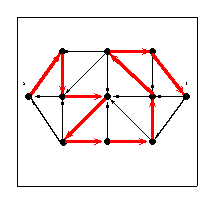
\includegraphics{./figs/rede}
\end{center} 
\end{floatingfigure}
\noindent


Uma certa empresa de telecomunica��es, cujo nome real n�o ser�
citado por raz�es de confidencialidade, mas que para nossa
comodidade ser� chamada de TeleMax, fornece linhas de transmiss�o
aos seus clientes de modo que estes possam, por exemplo, ligar-se
�s suas filiais por linhas privadas.
Para tal, conta com uma infra-estru\-tu\-ra de rede bastante complexa
compreendendo cabos e diversos equipamentos de jun��o.  Esta rede
� \textit{full-duplex}, ou seja, possui passagem de dados em ambos os
sentidos.  Para entender o processo de fornecimento de linhas de
transmiss�o, passaremos a um exemplo.  A empresa SoftSOF
possui duas sedes, uma em Santos e outra em Fernand�polis e, deseja interligar suas
filiais com uma qualidade m�nima de 200 Kbits/s, em pico de uso.
A SoftSOF possui 10 computadores em cada uma de suas filiais, logo
precisar�amos de um link de 200 Kbits/s $\times 10 = 2000$ Kbits/s.
� solicitado � TeleMax um \textit{link} de 2000 Kbits/s ligando as suas sedes.
A TeleMax n�o possui uma liga��o direta entre as duas cidades,
entretanto possui uma liga��o que passa por S�o Jos� do Rio
Preto, ou seja, um caminho Santos - S�o Jos� Do Rio Preto -
Fernand�polis.  Infelizmente, este link s� disp�e de 1024 Kbits/s.
No entanto, observando-se sua infra-estrutura, descobre-se que existe um outro
caminho: Santos - S�o Paulo - Fernand�polis, tamb�m com
capacidade de 1024 Kbits/s.  Pronto. A TeleMax pode fornecer o link
requerido pela SoftSOF, bastando para isso utilizar os dois
caminhos acima descritos, totalizando os 2048 Kbits/s, um pouco acima do requerido.

\par
\begin{figure}[htbp]
\begin{center}
\psfrag{Fernandopolis}{{\tiny Fernand�polis}}
\psfrag{Sao Paulo}{{\tiny S�o Paulo}}
\psfrag{Sao Jose do Rio Preto}{{\tiny S�o Jos� do Rio Preto}}
\psfrag{Santos}{{\tiny Santos}}
\psfrag{2000 Kbits}{{\tiny 2000 Kbits/s}}
\psfrag{1024 Kbits}{{\tiny 1024 Kbits/s}}
\psfrag{labela}{($a$)}
\psfrag{labelb}{($b$)}
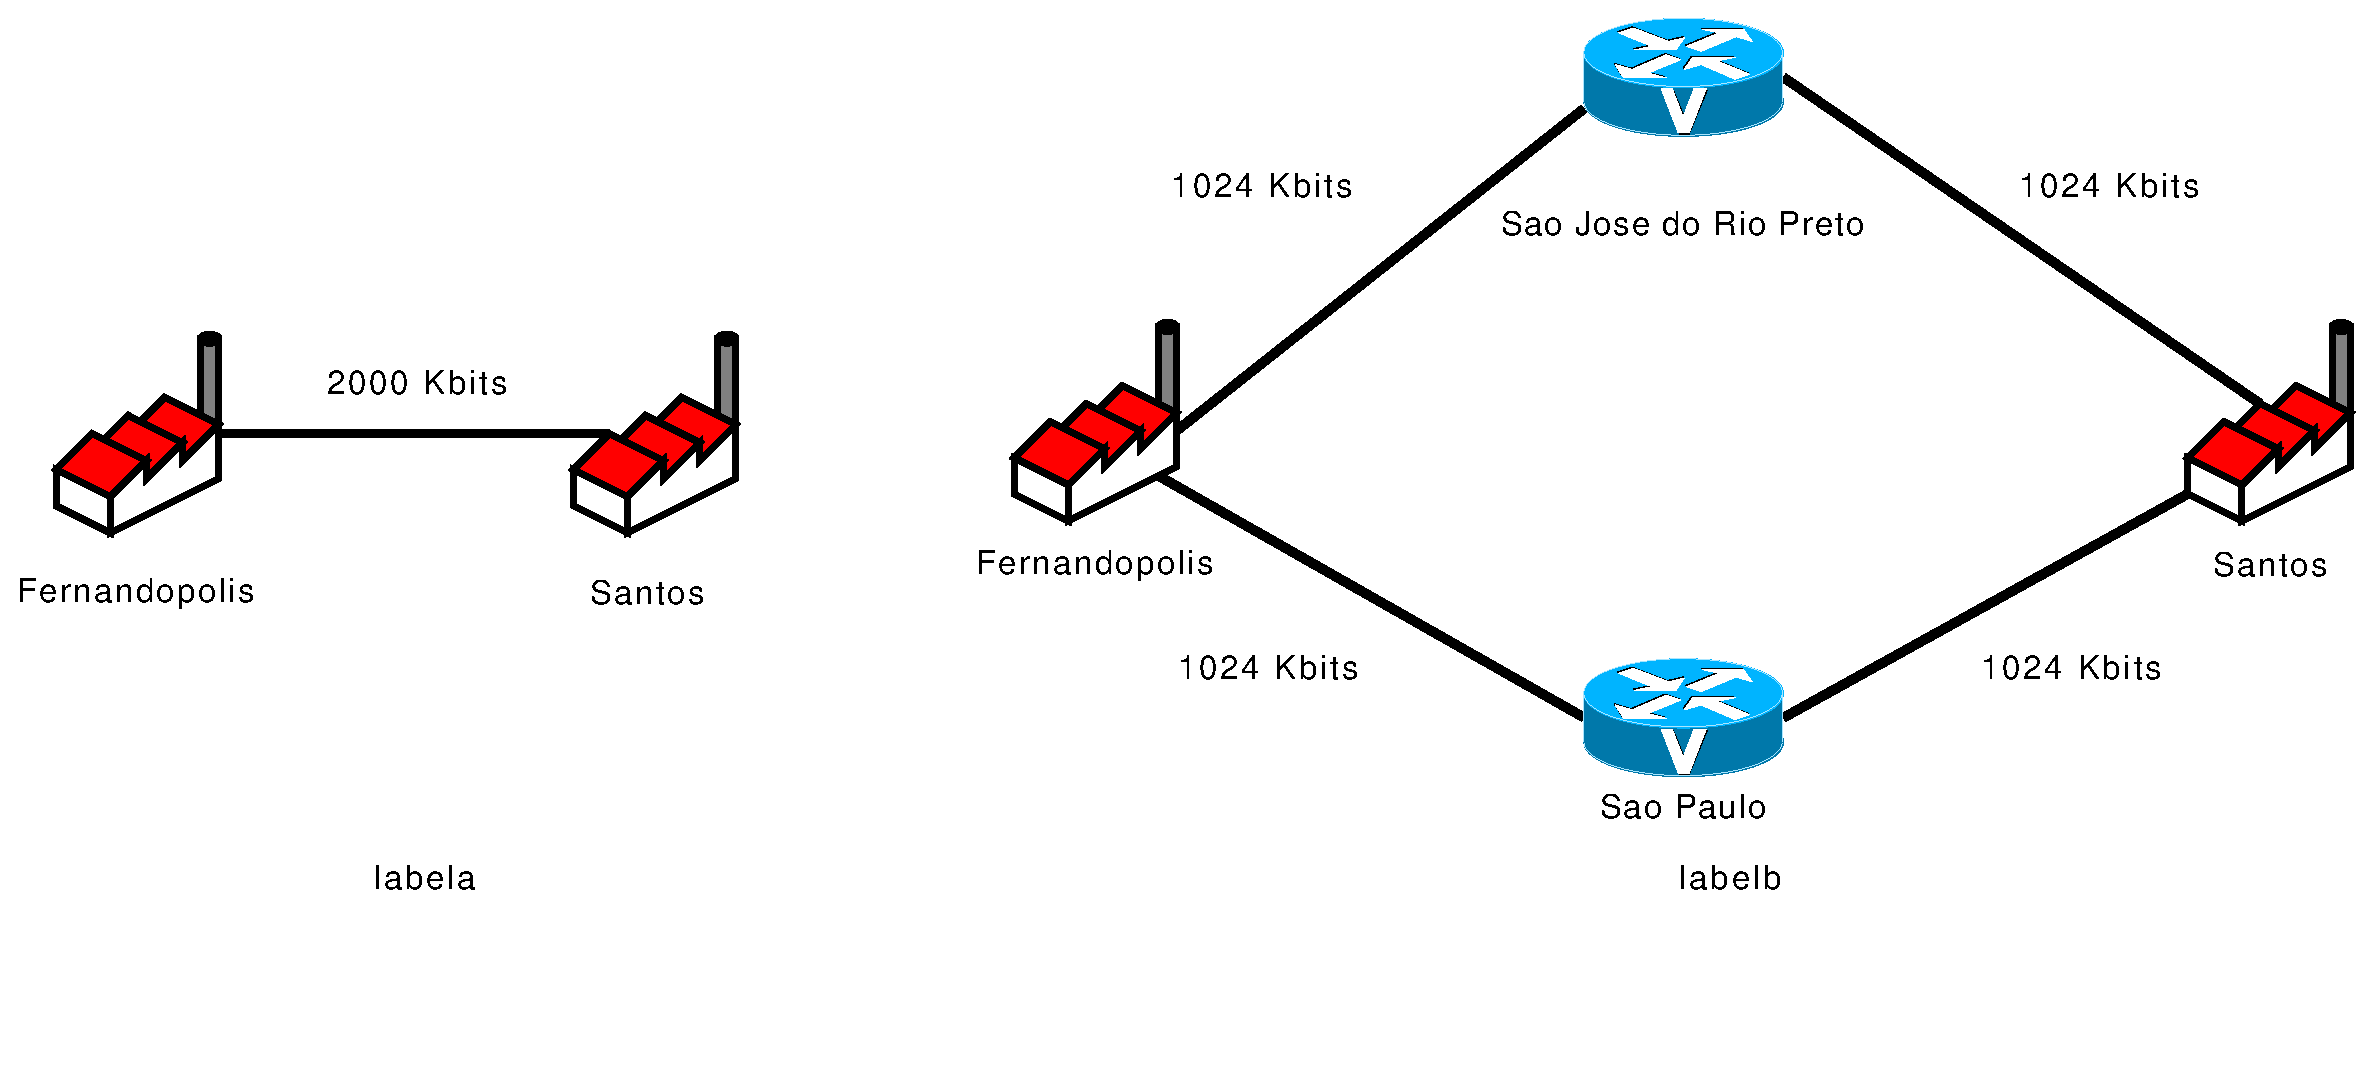
\includegraphics[width=1\textwidth]{./figs/introducaoTeleMax.eps}
   \caption{Em ($a$) vemos um esquema solicita��o da SoftSOF, um link de 2000 Kbits/s entre as filiais. Em ($b$) est� descrita a solu��o encontrada pela TeleMax, com base na disponibilidade de sua rede.}
\end{center} 
\end{figure}
\noindent
Vamos a algumas considera��es relevantes. O custo de um caminho � 
fun��o da quantidade de equipamentos usada e n�o da dist�ncia total 
dos cabos que o comp�e.
Isto se deve ao custo elevado dos equipamentos se comparado ao dos cabos. 
Assim, passa a ser melhor utilizar uma liga��o que percorra uma dist�ncia 
maior mas que passa por um n�mero menor de equipamentos, do que uma com 
menor dist�ncia mas que se utiliza de mais equipamentos.


A justificativa para a gera��o de diversos caminhos no lugar de apenas
um est� relacionada � capacidade de transmiss�o dispon�vel por cabo.  A
motiva��o para a gera��o dos menores caminhos, ou seja, com utiliza��o
m�nima de equipamentos, requer uma explica��o mais detalhada.  At� agora
fomos simplistas ao tratarmos das rela��es entre cabos e equipamentos
como se um equipamento se ligasse a apenas um cabo.  Na verdade, cada
equipamento se liga a um grande n�mero de cabos.  Assim, podemos ter
diversos caminhos entre dois equipamentos, um para cada cabo.  A fim de
utilizarmos bem os recursos da rede � interessante que o menor n�mero
de equipamentos esteja alocado para cada cliente pois, desta maneira, um
n�mero maior de liga��es poder� ser oferecido pela TeleMax.  Embora a
utiliza��o do menor n�mero poss�vel de equipamentos para cada cliente
n�o seja suficiente para garantir que a rede esteja sendo utilizada de
maneira eficiente, n�o nos importaremos com isto neste trabalho.  Feitas
as devidas considera��es, vamos agora justificar a automa��o do
processo.

Imagine levar a cabo o processo de fornecimento de linhas manualmente.  
Podemos salientar alguns problemas da abordagem manual.  Devido �s dimens�es da rede, o
operador respons�vel levar� muito tempo para obter uma lista de caminhos
entre os pontos.  Durante o tempo em que o operador gastar analisando a
rede, esta poder� ter sofrido altera��es, as quais n�o ser�o levadas em
conta por ele.  Al�m disso, sabemos como as pessoas s�o suscet�veis a
falhas, ainda mais quando expostas a atividades ma�antes e repetitivas.
Por conta destes fatores, a TeleMax sentiu a necessidade de uma
ferramenta computacional que gerasse de maneira r�pida e confi�vel uma
s�rie de caminhos entre dois pontos da sua rede.

Na constru��o da ferramenta, consideramos a rede
como um grafo sim�trico, por ser full-duplex, onde as arestas s�o
representadas pelos cabos e os v�rtices pelos equipamentos.  A
ferramenta tinha como n�cleo o algoritmo desenvolvido por Naoki Katoh,
Toshihide Ibaraki e H. Mine~\cite{katoh:n-12-411}, 
de gera��o de menores caminhos.  Os caminhos de mesmo custo,
ou seja, que se utilizam de igual quantidade de equipamentos, s�o
posteriormente reordenados crescentemente pela dist�ncia total
percorrida por seus cabos.  
Esta disserta��o trata de algoritmos que produzem caminhos de menor custo em grafos.
Embora algoritmos para tal sejam de interesse te�rico, � curioso
observar que foi uma aplica��o pr�tica, demandada por uma necessidade
surgida no �mbito empresarial, que nos levou ao estudo destes.


\section*{Organiza��o da disserta��o}


O cap�tulo~\ref{cap:preliminares} cont�m a maior parte das nota��es, conceitos e defini��es
que s�o usados ao longo desta disserta��o.

%%%%%%%%%%%%%%%%%%%%%%%%%%%%%%%%%%%%%%%%%%%%%%%%%%%%%%%%%%%%%%%%%%%%%%%%%
Em seguida, no cap�tulo~\ref{cap:problema-CM}, o m�todo de Dijkstra para gera��o de caminho m�nimo � descrito.

%%%%%%%%%%%%%%%%%%%%%%%%%%%%%%%%%%%%%%%%%%%%%%%%%%%%%%%%%%%%%%%%%%%%%%%%%
No cap�tulo~\ref{cap:problema-k-caminhos} descrevemos o problema dos $k$-menores caminhos.
Passamos, em seguida a descrever as �rvores de prefixos e finalizamos 
explicamos o algoritmo de YEN que as utiliza.

%%%%%%%%%%%%%%%%%%%%%%%%%%%%%%%%%%%%%%%%%%%%%%%%%%%%%%%%%%%%%%%%%%%%%%%%%
%, apresentando o algoritmo resultante, seu invariantes e uma
%an�lise de sua efici�ncia e corretude.
%%%%%%%%%%%%%%%%%%%%%%%%%%%%%%%%%%%%%%%%%%%%%%%%%%%%%%%%%%%%%%%%%%%%%%%%%
%No cap�tulo~4 o m�todo de YEN � descrito al�m da estrutura de �rvores de prefixos a partir do
%qual este pode ser melhor entendido.
%%%%%%%%%%%%%%%%%%%%%%%%%%%%%%%%%%%%%%%%%%%%%%%%%%%%%%%%%%%%%%%%%%%%%%%%%

Em seguida, no cap�tulo~\ref{cap:algoritmo-kim} o m�todo desenvolvido por Naoki Katoh,
Toshihide Ibaraki e H. Mine~\cite{katoh:n-12-411} � descrito detalhadamente.
Al�m disso, a implementa��o feita � exibida juntamente com uma simula��o de sua execu��o.
%%%%%%%%%%%%%%%%%%%%%%%%%%%%%%%%%%%%%%%%%%%%%%%%%%%%%%%%%%%%%%%%%%%%%%%%%

Seguimos, no cap�tulo~\ref{cap:experimentos} com uma s�rie de gr�ficos e 
an�lises experimentais do desempenho da nossa implementa��o do algoritmo de KIM.
%%%%%%%%%%%%%%%%%%%%%%%%%%%%%%%%%%%%%%%%%%%%%%%%%%%%%%%%%%%%%%%%%%%%%%%%%%

Finalmente, no cap�tulo~\ref{cap:consideracoes}, relatamos as nossas conclus�es, 
frustra��es e poss�veis trabalhos futuros.





%\section*{Breve cronologia}


 
%% A \defi{�rvore dos prefixos} de $\{P_1,\ldots,P_i\}$ � uma
%% �rvore enraizada junto com uma fun��o que associa um r�tulo a
%% cada n� e a cada aresta da �rvore. Suponha que 

%% Sejam $P_1,\ldots,P_i$ 
%% caminhos distintos de $s$ a~$t$ em um grafo, $V'$ e $A'$ 
%% o conjunto dos v�rtices e arcos presentes  nos caminhos, 
%% respectivamente.

%% Suponha que $(N,E)$ � uma �rvore com raiz $r$, conjunto de n�s $N$ 
%% e conjunto de arestas $E$. Suponha ainda que $f$ � uma fun��o 
%% r�tulo que associa a cada n� em $N$ um v�rtice em $V'$ e a cada aresta em $E$ 
%% um arco em $A$. Diremos que $(N,E,r,f)$ � uma \defi{�rvore dos caminhos}  
%% $\{P_1,\ldots,P_i\}$ se para cada caminho 
%%  \begin{eqnarray*}
%%  \seq{r=u_{0}, e_{1}, u_{1}, \ldots, e_{t}, u_{t}}
%%  \end{eqnarray*}
%% de $r$ a uma folha $u_t$ de $(N,E)$ temos que
%%  \begin{eqnarray*}
%%  \seq{f(r)=f(u_{0}), f(e_{1}), f(u_{1}), \ldots, f(e_{t}), u_{t}}
%%  \end{eqnarray*}
%% � um caminho em $\{P_1,\ldots,P_i\}$


%% Seja $\Rcal$ uma cole��o de caminhos em  
%% caminhos distintos em um grafo e sejam $V'$ e $A'$ 
%% o conjunto dos v�rtices e arcos presentes nos caminhos, 
%% respectivamente.

%% Suponha que $(N,E)$ � uma �rvore com raiz $r$, conjunto de n�s $N$ 
%% e conjunto de arestas $E$. Suponha ainda que $f$ � uma fun��o 
%% r�tulo que associa a cada n� em $N$ um v�rtice em $V'$ e a cada aresta em $E$ 
%% um arco em $A$. Se 
%% \begin{eqnarray*}
%%  Q=\seq{u_{0}, e_{1}, u_{1}, \ldots, e_{t}, u_{t}}
%% \end{eqnarray*}
%% � um caminho em  $(N,E)$, ent�o
%% \begin{eqnarray*}
%%  f(Q):=\seq{f(u_{0}), f(e_{1}), f(u_{1}), \ldots, f(e_{t}), u_{t}}
%% \end{eqnarray*}
%% Assim, $f(Q)$ � uma seq��ncia de v�rtices e arcos nos caminhos 

%% Diremos que $(N,E,r,f)$ � uma \defi{�rvore dos caminhos}  
%% $\Qcal$ se para cada caminho 
%%  \begin{eqnarray*}
%%  \seq{r=u_{0}, e_{1}, u_{1}, \ldots, e_{t}, u_{t}}
%%  \end{eqnarray*}
%% em $(N,E)$ de $r$ a uma folha $u_t$ corresponde a um �nico
%% caminho
%%  \begin{eqnarray*}
%%  \seq{f(r)=f(u_{0}), f(e_{1}), f(u_{1}), \ldots, f(e_{t}), u_{t}}
%%  \end{eqnarray*}
%% em $\Qcal$. Ademais, cada caminho em $\Qcal$  



 
%% um v�rtice em raiz 

%% que cada n� e cada aresta possui um r�tulo. Os
%% n�s s�o rotulados com v�rtices de


 


%% todos os caminhos em uma mesma 
%% parte t�m um prefixo comum. 





%%%%%%%%%%%%%%%%%%%%%%%%%%%%%%%%%%%%%%%%%%%%%%%%%%%%%%%%%%%%%%%%%%%%%%
%%
%%    CAP�TULOS
%%
%%%%%%%%%%%%%%%%%%%%%%%%%%%%%%%%%%%%%%%%%%%%%%%%%%%%%%%%%%%%%%%%%%%%%%

%%% Preliminares.
%%%%%%%%%%%%%%%%%%%%%%%%%%%%%%%%%%%%%%%%%%%%%%%%%%%%%%%%%%%%%%%%%%%%%%
%%
%%    PRELIMINARES
%%
%%%%%%%%%%%%%%%%%%%%%%%%%%%%%%%%%%%%%%%%%%%%%%%%%%%%%%%%%%%%%%%%%%%%%%

\chapter{Preliminares}
\label{cap:preliminares}
\markboth{Preliminares}{Preliminares}
%\addcontentsline{toc}{chapter}{Preliminares}

Neste cap�tulo apresentamos nota��es e defini��es que ser�o
extensivamente empregadas ao longo deste trabalho.

A maior parte das defini��es seguem de perto as empregadas por 
Paulo Feofiloff~\cite{pf:fluxos}.

%%%%%%%%%%%%%%%%%%%%%%%%%%%%%%%%%%%%%%%%%%%%%%%%%%%%%%%%%%%%%%%%%%%%%%%%%%%%
%%
%%  SE��O: NOTA��O B�SICA
%%
%%%%%%%%%%%%%%%%%%%%%%%%%%%%%%%%%%%%%%%%%%%%%%%%%%%%%%%%%%%%%%%%%%%%%%%%%%%% 
\section{Nota��o b�sica}



O conjunto dos n�meros inteiros ser� denotado por
$\Int$\index{$\Int$}\mar{$\Int$}. 
O conjunto dos n�meros inteiros n�o-negativos e positivos
$\NonnegInt$\index{$\NonnegInt$}\mar{$\NonnegInt$}.

� escrito $S$ uma \defi{parte}\index{parte} de um conjunto $V$ significando
que $S$ � um subconjunto de $V$.

Uma \defi{lista}\index{lista} � uma seq��ncia $\seq{v_1,v_2, \ldots, v_k}$ de
itens. 

Um \defi{intervalo}\index{intervalo} $[j\tdots k]$\index{$[j\tdots k]$}\mar{$[j\tdots k]$} �
uma seq��ncia de inteiros $j, j+1, \ldots,k$.  Se $i$ � um n�mero em $[j\tdots k]$,
ent�o $i$ � um n�mero inteiro tal que $j \leq i \leq k$.

%%%%%%%%%%%%%%%%%%%%%%%%%%%%%%%%%%%%%%%%%%%%%%%%%%%%%%%%%%%%%%%%%%%%%%%%%%%%
%%
%%  SE��O: GRAFOS, PASSEIOS E CAMINHOS
%%
%%%%%%%%%%%%%%%%%%%%%%%%%%%%%%%%%%%%%%%%%%%%%%%%%%%%%%%%%%%%%%%%%%%%%%%%%%%% 


\section{Grafos, passeios e caminhos}


Um \defi{grafo}\index{grafo} � um objeto da forma $(V,A)$, 
onde $V$ � um conjunto finito e $A$ � um conjunto de pares ordenados 
de elementos de $V$. 

Os elementos de $V$ s�o chamados \defi{v�rtices}\index{v�rtice@v�rtice} e os
elementos de $A$ s�o chamados \defi{arcos}\index{arco}.  Para cada arco
$(u,v)$, os v�rtices $u$ e $v$ representam a \defi{ponta inicial}\index{ponta!inicial} 
e a \defi{ponta final}\index{ponta!final} de
$(u,v)$, respectivamente.  

Um arco $(u,v)$ tamb�m ser� representado por
$uv$. Diremos que um tal arco \defi{sai} de $u$ e
\defi{entra} em $v$. 
O \defi{grau de entrada}\index{grau!entrada} 
de um v�rtice $v$ � o n�mero de arcos que entram em $v$; o \defi{grau
de sa�da}\index{grau!saida@sa�da} de $v$ � o n�mero de arcos que saem de $v$.

O conjunto de todos os arcos que t�m ponta inicial em um dado v�rtice $v$
� denotado por $A(v)$.\mar{$A(v)$}

Um grafo � \defi{sim�trico}\index{grafo!sim�trico@sim�trico} 
se para cada arco $uv$ existir tamb�m o arco $vu$. Diremos �s vezes
que o arco $vu$ � \defi{reverso}\index{arco!reverso}
do arco $uv$ e que o par $\{uv,vu\}$ � uma \defi{aresta}\index{aresta}.
 
Um grafo pode ser naturalmente representado atrav�s de um
diagrama, como o da figura~\ref{fig:grafo}, onde os v�rtices s�o
pequenas bolas e os arcos s�o as flechas ligando estas bolas. 

\begin{figure}[htbp]
 \begin{center}
    \psfrag{(a)}{$\iten{a}$}
    \psfrag{(b)}{$\iten{b}$}
    \psfrag{(c)}{$\iten{c}$}
    \psfrag{(d)}{$\iten{d}$}
    \psfrag{a}{{$a$}}
    \psfrag{b}{{$b$}}
    \psfrag{c}{{$c$}}
    \psfrag{d}{{$d$}}
    \psfrag{e}{{$e$}}   
    \psfrag{f}{{$f$}}
  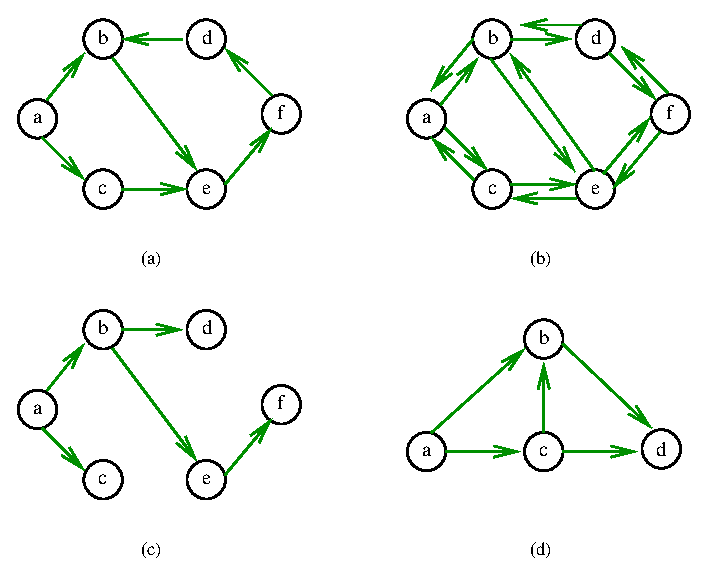
\includegraphics{./figs/grafo.eps}
  \caption[Exemplos de grafos e grafos sim�tricos]{\label{fig:grafo} $\iten{a}$, $\iten{b}$, $\iten{c}$ e 
    $\iten{d}$ s�o exemplos de grafos. $\iten{b}$ � um grafo sim�trico.}
 \end{center}
 \end{figure}



%%% Passeio 
 Um \defi{passeio}\index{passeio} num grafo $(V,A)$ � qualquer seq��ncia da forma
 \begin{eqnarray}
 \label{passeio}
 \seq{v_{0}, a_{1}, v_{1}, \ldots, a_{t}, v_{q}}
 \end{eqnarray}
onde $v_{0}, \ldots, v_{q}$ s�o v�rtices, $a_{1}, \ldots, a_{q}$ s�o
arcos e, para cada $i$, $a_{i}$ � um arco com ponta inicial $v_{i-1}$
e ponta final $v_{i}$.  O v�rtice $v_{0}$ � o
\defi{in�cio}\index{passeio!inicio@in�cio} ou \defi{ponta
  inicial}\index{passeio!ponta inicial} do passeio e o $v_{t}$ � seu
\defi{t�rmino}\index{passeio!termino@t�rmino} ou \defi{ponta
  final}.\index{passeio!ponta final} 

Um ciclo � um passeio onde $v_0=v_t$, ou seja come�a e termina no
mesmo v�rtice.  Um grafo � chamado de ac�clico se n�o possuir ciclos.
 

%Uma \defi{passeio n�o-orientado}\index{passeio! n�o orientado@n�o orientado}
%� uma seq��ncia como (\ref{passeio}) onde,
%para cada $i$, $\alpha_{i}$ � o arco $v_{i-1}v_{i}$ ou o arco
% $v_{i}v_{i-1}$. 
Na figura~\ref{fig:grafo}$\iten{a}$ a seq��ncia \\
$\seq{a, ab, b, be, e, ef, f, fd, d, db, b, be, e, ef, f}$ � um passeio 
com in�cio em $a$ e  t�rmino em $f$.
% e a seq��ncia $\seq{a, ac, c, ce, e, be, b, bd, d,df,f}$
% � um passeio n�o-orientado com in�cio em $a$ e t�rmino em $f$. 

%%%% 
Se $P:=\seq{v_{0}, a_{1}, v_{1}, \ldots, a_{t}, v_{q}}$ � um passeio, 
ent�o qualquer subseq��ncia da forma  
 \begin{eqnarray}
   \label{subpasseio}
   \seq{v_{i}, a_{i+1}, v_{i+1}, \ldots, a_{j}, v_{j}}
 \end{eqnarray}
com $0 \leq i \leq j \leq q$ ser� um
\defi{subpasseio}\index{subpasseio} de $P$.  Al�m disso, se $i=0$,
ent�o o subpasseio ser� dito um
\defi{prefixo}\index{prefixo}\index{subpasseio!prefixo} de $P$ e se
$j=q$ ent�o o subpasseio � dito um
\defi{sufixo}\index{sufixo}\index{subpasseio!sufixo} de $P$.  Na
figura~\ref{fig:grafo}$\iten{a}$ a seq��ncia $\seq{a, ab, b, be, e,
  ef, f, fd, d}$ � um subpasseio e prefixo de do passeio $\seq{a, ab,
  b, be, e, ef, f, fd, d, db, b, be, e, ef, f}$ e a seq��ncia
$\seq{e, ef, f, fd, d, db, b, be, e, ef, f}$ � um sufixo.


%%% Caminhos
Um \defi{caminho}\index{caminho} � um passeio
sem v�rtices repetidos. 
%Um \defi{caminho n�o-orientado}\index{caminho!n�o-orientado@n�o-orientado} 
%� um passeio n�o-orientado sem v�rtices repetidos.
Na figura~\ref{fig:grafo}$\iten{a}$ o passeio\\
 $\seq{a, ab, b, be, e, ef, f}$ � um caminho com in�cio em $a$ e 
 t�rmino em $f$.
% e a seq��ncia $\seq{a, ac, c, ce, e, be, b, bd, d, df,
% f}$ � um caminho n�o-orientado com in�cio em $a$ e t�rmino em $f$. 
Se num ciclo apenas a ponta inicial e a ponta final coincidem, 
ent�o dizemos que esse ciclo � um 
\defi{circuito}\index{circuito}. Na figura~\ref{fig:grafo}$\iten{a}$ o 
passeio $\seq{b, be, e, ef, f, fd, d, db, b}$ � um circuito. 

Por conveni�ncia, nossa defini��o de grafos n�o t�m "arcos paralelos":
dois arcos diferentes n�o podem ter a mesma ponta inicial e a mesma
ponta final.  Assim, podemos representar o passeio em (\ref{passeio})
simplesmente por
\[
 \seq{v_{0}, v_{1}, v_2, \ldots,  v_{q}}.
\]


\section{Grafos no computador}

Existem pelo menos tr�s maneiras populares de representar um grafo em um
computador, s�o elas: (1)~matriz de adjac�ncia; (2)~matriz de
incid�ncia e (3)~listas de adjac�ncia. Nesta 
disserta��o, matriz de adjac�ncia e listas de adjac�ncia s�o as
representa��o utilizadas.

% A seguir � decrita a representa��o de um grafo $(V,A)$ com $n$ v�rtices
% e $m$ arestas por meio de cada uma dessas estruturas.

% A seguir descrevemos como cada uma dessas representa��es 

\subsection*{Matriz de adjac�ncia}\index{matriz de!adjacencia@adjac�ncia}

Uma \defi{matriz de adjac�ncia} de um grafo $(V,A)$
� uma matriz com valores em $\{0,1\}$, e indexada por $V \times V$, onde
cada entrada $(u,v)$ da matriz tem valor $1$ se existe no grafo um arco de
$u$ a $v$, e $0$ caso contr�rio. Para grafos sim�tricos a matriz de
adjac�ncias � sim�trica.  O espa�o gasto com esta representa��o �
proporcional a $n^2$, onde $n$ � o n�mero de v�rtices do grafo.  Uma matriz de
adjac�ncia � mostrada na figura~\ref{fig:matriz_adj}. 


\begin{figure}[htbp]
 \centering
  \begin{tabular}{c|c|c|c|c|} 
   \multicolumn{1}{c}{} & 
   \multicolumn{1}{c}{$a$} & 
   \multicolumn{1}{c}{$b$} & 
   \multicolumn{1}{c}{$c$} & 
   \multicolumn{1}{c}{$d$}
   \\ \cline{2-5}
  $a$ & $0$ & $1$ & $1$ & $0$\\ \cline{2-5}
  $b$ & $0$ & $0$ & $0$ & $1$\\ \cline{2-5}
  $c$ & $0$ & $1$ & $0$ & $1$\\ \cline{2-5}
  $d$ & $0$ & $0$ & $0$ & $0$\\ \cline{2-5}
 \end{tabular}
  \caption{Matriz de adjac�ncia do grafo da figura~\ref{fig:grafo}$\iten{d}$.}
 \label{fig:matriz_adj}
\end{figure}

%\begin{figure}[htbp]
% \centering
% \begin{tabular}{cc}
%      &\begin{tabular}{cccc} $a$ & $b$ & $c$ & $d$ \\ \end{tabular} \\
%  $a$ &\begin{tabular}{|c|c|c|c|}\hline $0$ & $1$ & $1$ & $0$ \\\end{tabular}\\
%  $b$ &\begin{tabular}{|c|c|c|c|}\hline $0$ & $0$ & $0$ & $1$ \\\end{tabular} \\
%  $c$ &\begin{tabular}{|c|c|c|c|}\hline $0$ & $1$ & $0$ & $1$ \\\end{tabular}\\
%  $d$ &\begin{tabular}{|c|c|c|c|}\hline $0$ & $0$ & $0$ & $0$ \\\hline 
%       \end{tabular} \\
% \end{tabular}
%  \caption{Matriz de adjac�ncia do grafo da figura~\ref{fig:grafo}$\iten{d}$.}
% \label{fig:matriz_adj}
%\end{figure}


\subsection*{Matriz de incid�ncia}\index{matriz de!incidencia@incid�ncia}

Uma \defi{matriz de incid�ncia}  de um grafo $(V,A)$ �
uma matriz  com valores em \\ 
$\{-1,0,+1\}$ e indexada por $V \times A$, 
onde cada entrada $(u,a)$ � $-1$ se $u$ � ponta inicial de $a$, $+1$
se $u$ � ponta final de $a$, e $0$ caso contr�rio.
O espa�o gasto com esta representa��o �
proporcional a $nm$, onde $n$ � o n�mero de v�rtices e $m$ � o n�mero de
arcos do grafo. Uma matriz de incid�ncia da
figura~\ref{fig:grafo}$\iten{d}$ pode ser vista em ~\ref{fig:matriz_inc}.
Esta representa��o � par\-ti\-cu\-lar\-mente �til quando modelamos problemas de otimiza��o combinat�ria atrav�s de programas 
lineares~\cite{cook:co-1998,schrijver:cope-2003}.

\begin{figure}[htbp]
 \centering
  \begin{tabular}{r|r|r|r|r|r|} 
   \multicolumn{1}{c}{} & 
   \multicolumn{1}{c}{$ab$} & 
   \multicolumn{1}{c}{$ac$} & 
   \multicolumn{1}{c}{$cb$} & 
   \multicolumn{1}{c}{$cd$} & 
   \multicolumn{1}{c}{$bd$}
   \\ \cline{2-6}
  $a$ & $-1$ & $-1$ & $0$ & $0$ &$0$ \\ \cline{2-6}
  $b$ & $+1$ & $0$ & $+1$ & $0$ & $-1$ \\ \cline{2-6}
  $c$ & $0$ & $+1$ & $-1$ &$-1$ &$0$ \\ \cline{2-6}
  $d$ & $0$ & $0$ & $0$ & $+1$ & $+1$\\ \cline{2-6}
 \end{tabular}
  \caption{Matriz de incid�ncia do grafo da figura~\ref{fig:grafo}$\iten{d}$.}
 \label{fig:matriz_inc}
\end{figure}
 
\subsection*{Listas de adjac�ncia}\index{listas de!adjacencia@adjac�ncia}


Na representa��o de um grafo $(V,A)$ atrav�s de \defi{listas de 
adjac�ncia} tem-se, para cada v�rtice $u$, 
uma lista dos arcos com ponta inicial $u$. 
Desta forma, para cada v�rtice $u$, o conjunto $A(u)$ � 
representado por uma lista.
O espa�o gasto com esta representa��o �
proporcional a $n+m$, onde $n$ � o n�mero de v�rtices e $m$ � o n�mero de
arcos do grafo. Uma lista de adjac�ncia est� ilustrada na
figura~\ref{fig:lista_adj}.

\begin{figure}[htbp]
 \centering
 \begin{tabular}{ccc}
   $A(a)$: & $ab$, & $ac$ \\
   $A(b)$: & $bd$  &      \\
   $A(c)$: & $cb$, & $cd$ \\
   $A(d)$: &       &      \\
 \end{tabular}
  \caption{Listas de adjac�ncia do grafo da figura~\ref{fig:grafo}$\iten{d}$.}
 \label{fig:lista_adj}
\end{figure}
 

%%%%%%%%%%%%%%%%%%%%%%%%%%%%%%%%%%%%%%%%%%%%%%%%%%%%%%%%%%%%%%%%%%%%%%%%%%%%
%%
%%  SE��O:  FILAS DE PRIORIDADE
%%
%%%%%%%%%%%%%%%%%%%%%%%%%%%%%%%%%%%%%%%%%%%%%%%%%%%%%%%%%%%%%%%%%%%%%%%%%%%% 
\section{Filas de prioridade} 
\label{sec:filadeprioridade}

Sempre que representamos dados em um computador n�s consideramos
cada um dos seguintes aspectos:
\begin{enumerate}
 \item[$\iten{1}$] a maneira que essas informa��es (ou objetos do
 mundo real) s�o modelados como objetos matem�ticos; 
 \item[$\iten{2}$] o conjunto de opera��es que definiremos sobre estes
 objetos matem�ticos; 
 \item[$\iten{3}$] a maneira na qual estes objetos ser�o armazenados
 (representados) na mem�ria de um computador; 
 \item[$\iten{4}$] os algoritmos que s�o usados para executar as
 opera��es sobre os objetos com a representa��o escolhida. 
\end{enumerate}
Para prosseguir, precisamos entender a diferen�a entre
 os seguintes termos, tipo de dados, tipo abstrato de dados e estrutura de dados.
 
O \defi{tipo de dado}\index{tipo!de dado} de uma vari�vel � o conjunto
de valores que esta vari�vel pode assumir.  Por exemplo, uma vari�vel
do tipo boolean s� pode assumir os valores \textsc{true} e
\textsc{false}.

Os itens $\iten{1}$ e $\iten{2}$ acima dizem respeito ao
\defi{tipo abstrato de dados}%
\index{tipo!abstrato de dados}, ou seja, ao modelo matem�tico junto com uma
cole��o de opera��es 
definidas sobre este modelo. Um exemplo de tipo abstrato de dados � o conjunto 
dos n�meros inteiros com as opera��es de \textit{adi��o}, \textit{subtra��o}, 
\textit{multiplica��o} e \textit{divis�o} sobre inteiros. 

J� os itens $\iten{3}$ e $\iten{4}$ est�o relacionados aos
aspectos de implementa��o. 

Para representar um tipo abstrato de dados em um computador n�s usamos uma 
\defi{estrutura de dados}\index{estrutura de dados}, que � uma cole��o
de vari�veis, 
possivelmente de diferentes tipos, ligadas (relacionadas) de diversas maneiras. 

 Uma \defi{fila de prioridades}\index{fila de!prioridades}%
~\cite{ahuja:netflows, clr:introalg-1999}
 � um tipo abstrato de dados que consiste de 
uma cole��o de itens, cada um com um valor ou prioridade associada.
Nos algoritmos tratados neste texto os itens ser�o, basicamente, v�rtices.

 Uma fila de prioridade tem suporte para as seguintes opera��es:
\begin{itemize}
\item $\Insert (v, val)$: adiciona o v�rtice $v$ com valor $val$
na cole��o.\index{Insert@\Insert}
\item $\Delete(v)$: remove o v�rtice $v$ da cole��o.\index{Delete@\Delete}
\item $\ExtractMin (~)$: devolve o v�rtice com o menor valor 
e o remove da cole��o.\index{ExtractMin@\ExtractMin}
\item $\DecreaseKey (v, \val)$: muda para $\val$ o valor associado
ao v�rtice $v$; assume-se que $\val$ n�o � maior que o valor corrente
associado a $v$. Note que  \DecreaseKey{} sempre pode ser
implementada como um \Delete{}
seguido por um \Insert{}.\index{DecreaseKey@\DecreaseKey}
\end{itemize}

 Uma seq��ncia de opera��es � chamada \defi{mon�tona}%
\index{operacoes monotona@opera��es mon�tonas}
se os valores retornados por sucessivos \ExtractMin's s�o
n�o-decrescentes.
O algoritmo \Dijkstra{} (se��o~\ref{sec:dijkstra}) 
executa uma seq��ncia mon�tona de opera��es sobre os v�rtices de um grafo.



\section{Java Universal Network/Graph Framework}
\lstset{basicstyle=\footnotesize,numbers=left, numberstyle=\tiny,
  stepnumber=1,breaklines=true} O Java Universal Network/Graph
Framework (JUNG) � uma biblioteca de software livre, escrita em Java,
desenvolvida para permitir a modelagem, an�lise e visualiza��o de
dados pass�veis de serem representados na forma de grafos.  Al�m de
permitir a visualiza��o de grafos, conta com diversos algoritmos
implementados e estruturas de dados pertinentes � �rea de grafos.

A biblioteca foi criada de modo a abranger as mais diversas
necessidades, sendo assim bastante gen�rica, capaz de representar
grafos na forma de matrizes e listas de adjac�ncia e tratar de grafos
e grafos sim�tricos.  No n�vel mais elevado, ou seja, de maior
abstra��o, temos as interfaces com prefixo Archetype, as quais definem
as diretrizes dos tipos mais gen�ricos de elementos componentes de um
grafo: v�rtices, arcos e o grafo em si.  S�o representantes deste
n�vel as interfaces: \lstinline{ArchetypeGraph},
\lstinline{ArchetypeVertex} e \lstinline{ArchetypeEdge}.


No n�vel imediatamente inferior, especializando as interfaces
anteriores, encontramos as interfaces: \lstinline{Graph},
\lstinline{Vertex} e \lstinline{Edge}.  Estas objetivam representar
elementos de grafos sem arestas paralelas, uma vez que estes permitem
que novos opera��es sejam definidas.


Para se trabalhar com grafos e grafos sim�tricos, distinguindo-os dos
demais, foram criadas duas interfaces: \lstinline{DirectedGraph} e \lstinline{UndirectedGraph} e as
respectivas \lstinline{DirectedEdge} (arco) e
\lstinline{UndirectedEdge} (aresta).  Estas interfaces permitem
valida��es em tempo de compila��o.  Nenhuma delas possui m�todos
pr�prios, apenas estendem a interface \lstinline{Graph}.  A valida��o
em tempo de compila��o ocorre por conta da compara��o entre a
assinatura das fun��es que as utilizam.  Se uma dada fun��o possuir na
sua assinatura um par�metro do tipo \lstinline{UndirectedGraph} e for
invocada com um argumento do tipo \lstinline{DirectedGraph} teremos um
erro de compila��o.  Observe, no entanto, que a interface
\lstinline{UndirectedGraph} por si s� n�o valida a simetria do grafo.
Esta valida��o fica a cargo da implementa��o da mesma.


A seguir temos as implementa��es das interfaces citadas acima.  Numa
camada intermedi�ria, existem tr�s classes abstratas implementando
funcionalidades comuns a grafos e grafos sim�tricos, s�o elas:
\lstinline{AbstractSparseGraph}, \lstinline{AbstractSparseVertex}
e \newline \lstinline{AbstractSparseEdge}.  No momento, apenas temos
implementada a representa��o de grafos como listas de adjac�ncia, como
pode ser notado nos pr�prios nomes das classes, os quais cont�m a
palavra \emph{Sparse}; vale lembrar que grafos esparsos, ou seja, com
poucos arcos, se comparado � quantidade m�xima poss�vel, s�o, em
geral, representados de maneira mais eficiente e econ�mica usando-se
listas de adjac�ncia e grafos densos como matrizes de adjac�ncia.
 
Por fim, temos as implementa��es espec�ficas para grafos: 
\lstinline{DirectedSparseGraph}, \newline 
\lstinline{DirectedSparseVertex} e \lstinline{DirectedSparseEdge},
e grafos sim�tricos: \lstinline{UndirectedSparseGraph}, \newline \lstinline{UndirectedSparseVertex} e \lstinline{UndirectedSparseEdge}.

\subsection*{Cria��o de grafos e grafos sim�tricos}

Visto um pouco da arquitetura vamos passar a alguns exemplos e aplica��es.
Criar um grafo � um processo bem simples, basta instar a classe referente ao tipo grafo 
desejado, como no exemplo a seguir:
%\lstset{basicstyle=\small,tabsize=2,xleftmargin=.5cm,xrightmargin=.5cm}
\lstset{numbers=none}
\begin{lstlisting}
	Graph g = new DirectedSparseGraph();
\end{lstlisting}
cria um grafo baseado numa representa��o na forma de lista de adjac�ncia,
\begin{lstlisting}
	Graph g = new UndirectedSparseGraph();
\end{lstlisting}
cria um grafo sim�trico baseado numa representa��o na forma de lista de adjac�ncia.

Uma vez criado o grafo, podemos adicionar-lhe v�rtices da seguinte forma:
\lstset{language=Java,caption={}}
\begin{lstlisting}
	Vertex v1 = (Vertex) new DirectedSparseVertex();
	Vertex v2 = (Vertex) new DirectedSparseVertex();
	g.addVertex(v1);
	g.addVertex(v2);
\end{lstlisting}
e depois adicionar-lhe os arcos:
\lstset{language=Java,caption={}}
\begin{lstlisting}
	DirectedEdge e = (DirectedEdge) new DirectedSparseEdge(v1, v2);
	g.addEdge(e);
\end{lstlisting}

Observe nos exemplos acima que tanto arcos quanto v�rtices s�o independentes do grafo: 
primeiramente s�o criados e s� ent�o adicionados a ele.
Algumas observa��es importantes:
\begin{itemize}
\item um v�rtice/arco s� pode pertencer a um grafo;
\item um v�rtice/arco s� pode ser adicionado uma vez a um grafo;
\item a direcionalidade de um v�rtice deve coincidir com a do grafo no qual ele ser� inserido.
Por exemplo, n�o � poss�vel adicionar um v�rtice \lstinline{DirectedSparseVertex} a uma implementa��o de 
\lstinline{UndirectedGraph};
\item a direcionalidade de um arco deve coincidir com a dos v�rtices que este conecta e 
tamb�m com a do grafo.
\end{itemize}

Tamb�m � poss�vel criar um grafo a partir de dados de um arquivo. 
Apresentaremos apenas um exemplo usando o padr�o Pajek~\cite{jung:pajek} 
uma vez que o JUNG � capaz de ler e escrever apenas neste formato
(o formato GraphML � suportado somente no modo leitura).
O formato Pajek � muito abrangente, permitindo defini��es bem complexas de grafos, contudo apresentaremos
apenas alguns exemplos simples de seu uso.

Come�aremos mostrando um arquivo no formato Pajek representando
um grafo sim�trico com 14 v�rtices, sem custos nas arestas:
\lstset{basicstyle=\footnotesize,numbers=left, numberstyle=\tiny, stepnumber=1}
\begin{lstlisting}
	*Vertices 14
	1 I1
	2 I3
	3 W1
	4 W2
	5 W3
	6 W4
	7 W5
	8 W6
	9 W7
	10 W8
	11 W9
	12 S1
	13 S2
	14 S4
	*Edges
	1 5
	3 5
	3 6
	5 6
	9 10
	9 11
	10 11
	3 12
	5 12
	6 12
	10 14
	11 14
	9 12
\end{lstlisting}

Os v�rtices s�o numerados a partir do 1.
Cada v�rtice pode possuir um r�tulo, que deve vir ap�s seu n�mero, por exemplo, 
o v�rtice n�mero 2 tem o r�tulo \emph{I3}.
Para definir as arestas usamos *Edges, como exibido na linha~16.
Cada aresta � definida pelos dois v�rtices que conecta, por exemplo, na linha~17
temos uma aresta conectando os v�rtices 1 e 5.
Vale lembrar que o arquivo n�o pode conter linhas em branco.

A figura a seguir mostra uma ilustra��o do grafo sim�trico descrito acima.

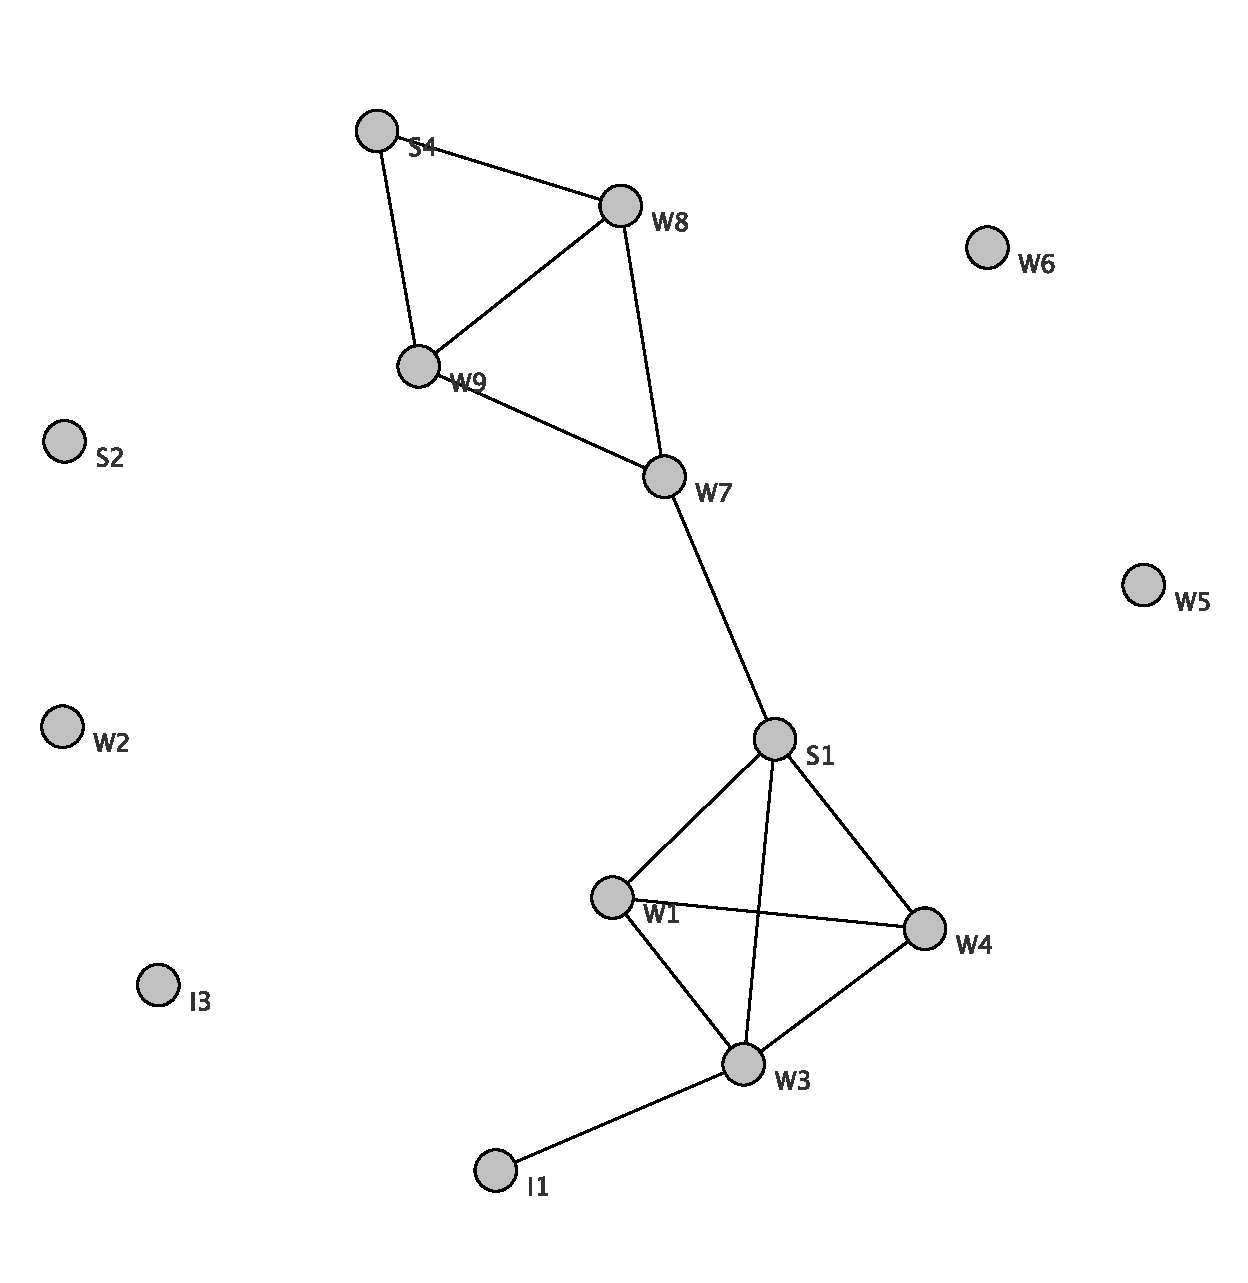
\includegraphics[scale=0.5]{./figs/grafoSimetricoSemCustos.eps} 

Agora vamos criar um grafo sim�trico como o anterior, mas com custos em suas arestas:
\begin{lstlisting}
	*Vertices 14
	1 I1
	2 I3
	3 W1
	4 W2
	5 W3
	6 W4
	7 W5
	8 W6
	9 W7
	10 W8
	11 W9
	12 S1
	13 S2
	14 S4
	*Edges
	1 5 1
	3 5 2.9
	3 6 3
	5 6 90
	9 10 1
	9 11 2
	10 11 3
	3 12 66
	5 12 6.7
	6 12 21
	10 14 2
	11 14 33
	9 12 1
\end{lstlisting}

Observe que as arestas cont�m tr�s n�meros, onde os dois primeiros correspondem aos v�rtices que ela conecta
e o terceiro ao seu custo. 
Por exemplo, na linha~18, temos a aresta conectando os v�rtices 3 e 5 com custo 2.9.

A figura a seguir mostra uma ilustra��o do grafo sim�trico descrito acima.

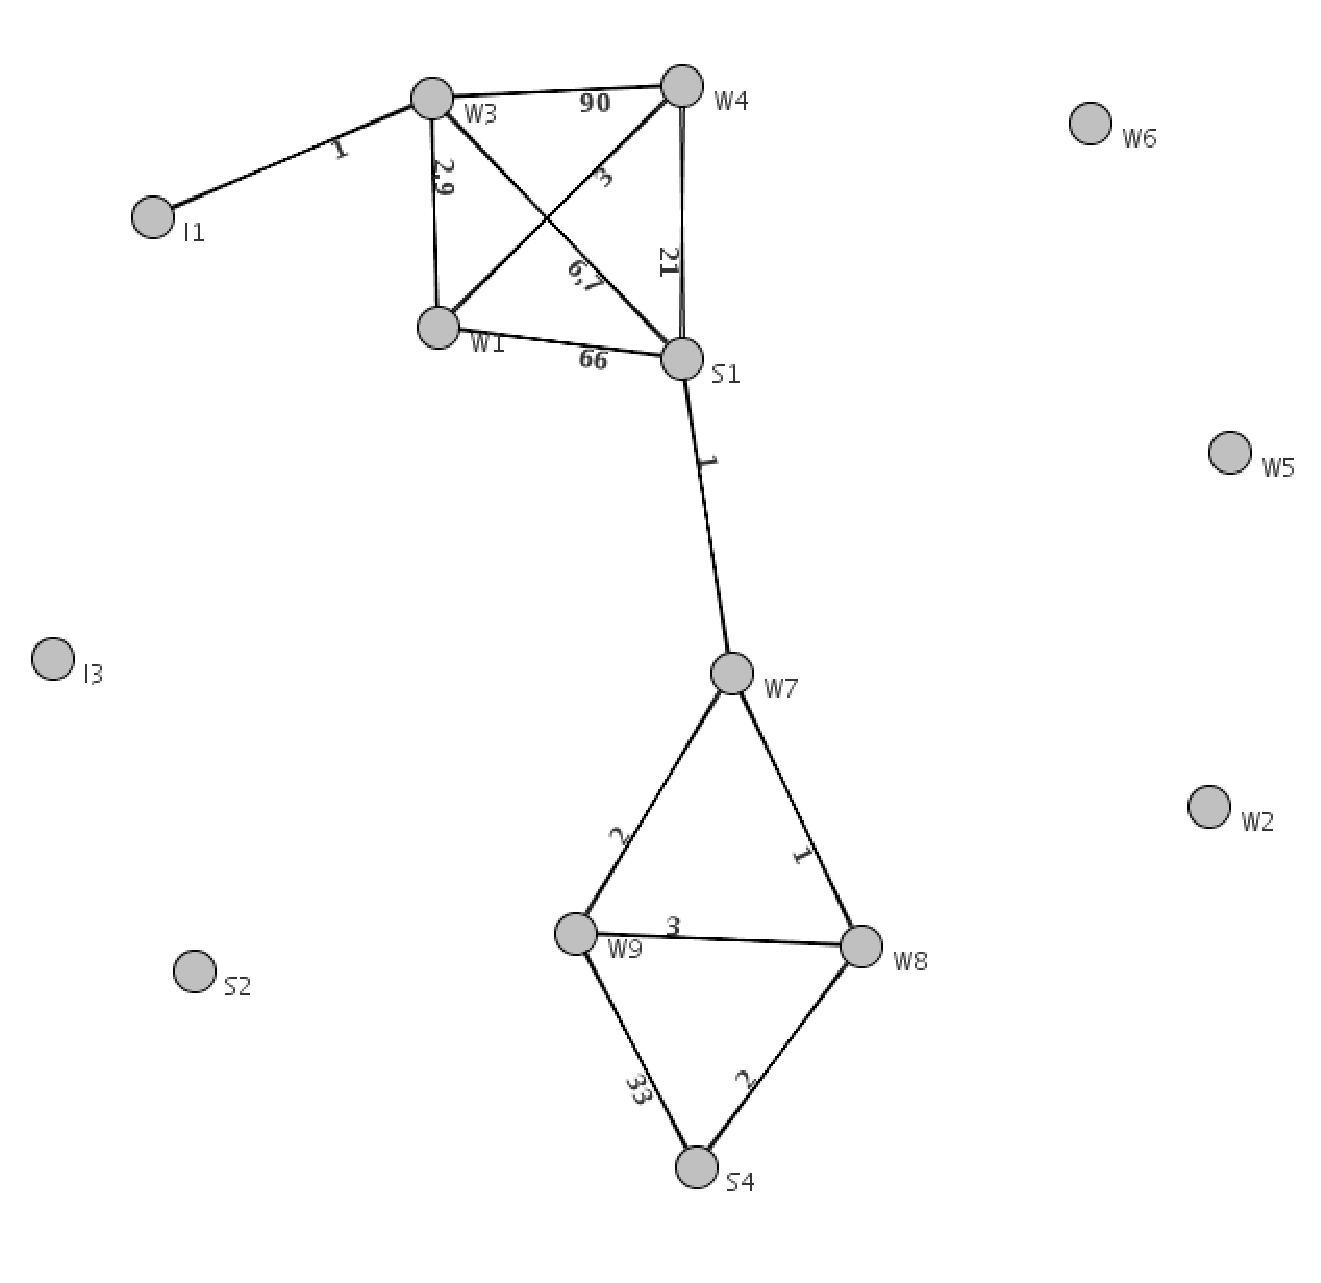
\includegraphics[scale=0.5]{./figs/grafoSimetricoComCustos.eps} 

A cria��o de grafos � um pouco diferente.
Lembramos que em nosso trabalho estamos apenas interessados em grafos sim�tricos.
No entanto, apenas � t�tulo de curiosidade, exibiremos um exemplo.

A seguir temos a descri��o de um grafo com 19 v�rtices, sem custo nos arcos:
\begin{lstlisting}
	*Vertices 19
	*Arcslist
	1 4 6 17 5 13 12 9 8 7
	3 13 12 8 7
	4 6 5 9
	2 6 5
	13 16
	12 16
	9 16
	9 19
	8 16 18
	7 16 18
	15 16 19
	14 16 19
	6 18
	5 18
	16 19 18
	11 18
	10 18
\end{lstlisting}

Observe que n�o h� nenhuma linha contendo o n�mero do v�rtice seguido de seu r�tulo.
Sendo assim, assume-se que os v�rtices s�o numerados de 1 a 19 e rotulados de V0 a V18.
Note que o v�rtice de n�mero 1 n�o � necessariamente rotulado por V0, 2 por V1, e assim por diante.
No nosso exemplo, o v�rtice 3 � rotulado como V17.
A defini��o dos arcos � um pouco diferente do que vimos anteriormente quando trabalhamos com grafos sim�tricos e arestas.
Em primeiro lugar, usamos *Arcslist no lugar de *Edges e,
uma vez que nosso grafo n�o tem custo nos arcos, 
podemos defini-los em fun��o dos v�rtices adjacentes.
Por exemplo, na linha~4 definimos arcos que conectam o v�rtice 3 aos v�rtices: 13, 12, 8 e 7.

A figura a seguir mostra uma ilustra��o do grafo descrito acima.

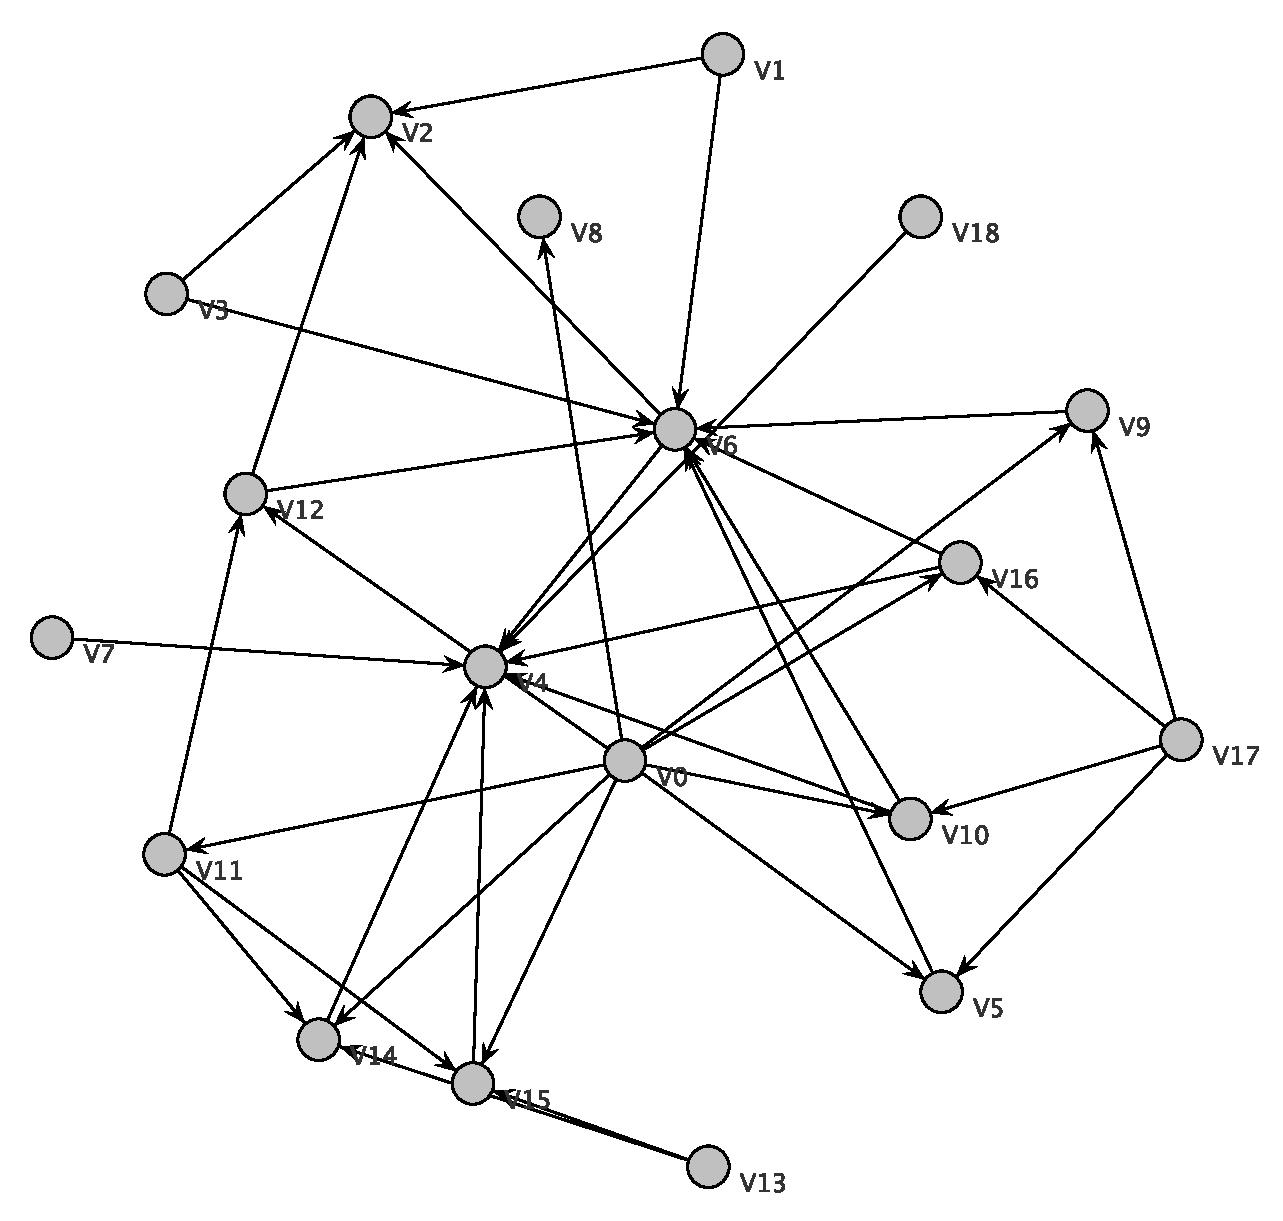
\includegraphics[scale=0.5]{./figs/grafoAssimetricoSemCustos.eps} 

A leitura de um arquivo contendo um grafo ou grafo sim�trico no formato Pajek consiste dos seguintes passos:
\begin{enumerate}[(1)]
\item cria��o de um leitor PajekNet;
\item cria��o de um objeto a partir de uma classe referente ao tipo de grafo desejado.
Lembre-se que temos grafos e grafos sim�tricos;
\item defini��o da maneira pela qual os custos s�o atribu�dos �s arestas ou aos arcos.
\end{enumerate}

O trecho de c�digo a seguir ilustra os passos descritos acima:
\lstset{language=Java,caption={}}
\begin{lstlisting}
	PajekNetReader pajekNetReader = new PajekNetReader(false);
	UndirectedGraph g = new UndirectedSparseGraph();
	NumberEdgeValue nev = new UserDatumNumberEdgeValue(g);
	g = (UndirectedGraph) pajekNetReader.load("data/pajNetTest.dat", g, nev); 
\end{lstlisting}		

Na linha~1 temos a cria��o do leitor PajekNet, usando a classe \lstinline{PajekNetReader}.
Na linha~2 criamos o objeto \lstinline{g} referente a um grafo sim�trico.
Em seguida, na linha~3 de\-fi\-ni\-mos como os custos s�o atribu�dos aos v�rtices, neste caso 
o reposit�rio~\footnote{O reposit�rio do usu�rio ser� apresentado quando tratarmos do 
armazenamento de informa��es nos elementos contituintes de um grafo na se��o Anota��es.}
do usu�rio cont�m esses custos, os quais s�o lidos do arquivo PajekNet.
Finalizamos, na linha~4, criando o grafo sim�trico a partir dos dados do arquivo: \lstinline{data/pajNetTest.dat}.

\subsection*{Atribui��o de custos �s arestas ou aos arcos}

O JUNG permite flexibilidade na maneira como os custos s�o atribu�dos aos arcos e �s arestas.
Para tal, existe a interface \lstinline{NumberEdgeValue} que define dois m�todos: \lstinline{getNumber} e \lstinline{setNumber}.
A id�ia � deixar o desenvolvedor livre para criar qualquer tipo de implementa��o 
que defina os custos dos arcos/arestas do seu grafo/grafo sim�trico.
A  biblioteca JUNG j� conta com quatro implementa��es desta interface: \lstinline{ConstantDirectionalEdgeValue},
 \lstinline{ConstantEdgeValue}, \lstinline{EdgeWeightLabeller} e \lstinline{UserDatumNumberEdgeValue}
Em nosso trabalho usamos apenas duas dessas:

\lstinline{ConstantEdgeValue}: define todos os arcos como tendo o mesmo custo;

\lstinline{UserDatumNumberEdgeValue}: obt�m os custos dos arcos no reposit�rio de dados do usu�rio.


Caso o grafo tenha sido obtido a partir de um arquivo no formato Pajek contendo 
custos devemos usar \lstinline{UserDatumNumberEdgeValue}.

\subsection*{Armazenando dados no grafo}

Citamos, anteriormente, o reposit�rio de dados do usu�rio, o qual � apenas uma das formas 
disponibilizadas pelo JUNG para permitir ao usu�rio armazenar dados no grafo.
Al�m disso, � poss�vel adicionar dados aos arcos (grafo), arestas (grafo sim�trico) e v�rtices.
Para isso, o usu�rio pode optar por especializar uma classe que implemente a 
interface \lstinline{ArchetypeVertex} ou utilizar os m�todos de anota��es oferecidos. 
Explicaremos melhor como funcionam estes dois m�todos a seguir:
\subsubsection*{Especializa��o}
Suponha que cada v�rtice contenha um nome.
Usando-se especializa��o de classes, o usu�rio pode criar a classe \lstinline{MeuVertice} 
contendo o atributo nome e m�todos que definam e obtenham este dado, 
como � mostrado no exemplo a seguir:
\lstset{language=Java,tabsize=2,caption=,numbers=left, numberstyle=\tiny, stepnumber=1, numbersep=5pt,basicstyle=\footnotesize,showstringspaces=false}
\begin{lstlisting}[name=Especializa��o da classe DirectedSparseVertex]
class MeuVertice extends DirectedSparseVertex {
    private String nome;

    public MeuVertice( String nome ) {
       this.nome = nome;
    }

	 public String getNome(){
	 	 return nome;
	 }
	 
	 public void setNome(String nome){
	 	 this.nome=nome;
	 }
}
\end{lstlisting}
\subsubsection*{Anota��es}
\label{subsec:anotacoes}
Podemos realizar a mesma tarefa utilizando uma solu��o bem mais flex�vel: anota��es.
Cada uma das implementa��es das interfaces \lstinline{Vertex}, \lstinline{Edge} e \lstinline{Graph} implementa tamb�m a 
interface \lstinline{UserData} a qual define opera��es 
que permitem adicionar dados a cada um dos elementos do grafo. 
S�o elas:

\lstinline{addUserDatum(key, datum, copyaction)}: adiciona o objeto \lstinline{datum} usando o objeto \lstinline{key} como chave al�m de especificar o \lstinline{copyaction};

\lstinline{getUserDatum(key):} obt�m o objeto armazenado com a chave \lstinline{key};

\lstinline{removeUserDatum(key):} remove o objeto armazenado com a chave \lstinline{key};

\lstinline{setUserDatum(key, datum, copyaction):} adiciona ou substitui o objeto cuja chave seja \lstinline{key}, al�m de redefinir o \lstinline{copyaction};

\lstinline{importUserData(udc):} importa os dados do reposit�rio de usu�rio armazenado em \lstinline{udc};

\lstinline{getUserDatumKeyIterator():} retorna um objeto de itera��o que permite navegar pelos dados armazenados pelo usu�rio no seu reposit�rio;

\lstinline{getUserDatumCopyAction(key):} retorna o \lstinline{copyaction} especificado pelo usu�rio para o objeto armazenado segundo a chave \lstinline{key}. 

Adicionando a informa��o nome a um v�rtice:
\lstset{language=Java,caption={}}
\begin{lstlisting}
	Vertex v = (Vertex) g.addVertex(new DirectedSparseVertex());
	v.addUserdatum("nome","Pisaruk",UserData.SHARED);
	g.addUserdatum("id","10",UserData.CLONE);
\end{lstlisting}

Quando um grafo ou qualquer de seus elementos constituintes � copiado, o destino dos dados do 
reposit�rio do usu�rio de cada um deles � determinado pelo seu \lstinline{copyaction}.
O JUNG fornece tr�s diferentes solu��es, sendo que o usu�rio pode criar 
outras implementando a interface \lstinline{CopyAction}, s�o elas: 

\lstinline{UserData.CLONE:} retorna uma c�pia dos dados armazenados segundo a implementa��o do m�todo clone(), 
definido na classe \lstinline{Object} do Java;

\lstinline{UserData.REMOVE:} retorna \lstinline{null}, ou seja, o dado n�o � copiado;

\lstinline{UserData.SHARED:} retorna uma refer�ncia ao objeto armazenado, ou seja, qualquer mudan�a ser� refletida nas duas refer�ncias.

\subsection*{Mudan�as na vers�o 2.0 do JUNG}

Quando iniciamos a implementa��o do algoritmo KIM em Java usamos a vers�o mais recente da biblioteca JUNG naquele momento,
ou seja, a vers�o 1.7.
Pouco antes da finaliza��o, a vers�o 2.0 foi disponibilizada e decidimos us�-la por diversos motivos, dentre eles:
\begin{itemize}
\item Flexibilidade para usar qualquer classe como v�rtice ou arco.
Na vers�o anterior era preciso trabalhar com as interfaces \lstinline{AchetypeVertex} e \lstinline{ArchetypeEdge};
\item Simplifica��o da arquitetura de classes;
\item Uso de \emph{Generics} do Java.
\end{itemize}

Para come�ar, temos a interface \lstinline{Graph<V,E>} a qual define as opera��es b�sicas que podem ser realizadas em um grafo, 
dentre elas:
\begin{itemize}
\item Adi��o e remo��o de v�rtices e/ou arcos;
\item Obten��o das pontas de um arco, ou seja, os v�rtices que este conecta;
\item Obten��o de informa��es referentes aos v�rtices, tais como: grau, predecessores e sucessores.
\end{itemize}

H� tamb�m tr�s interfaces que especializam a interface \lstinline{Graph<V,E>}:

\lstinline{DirectedGraph<V, E>}: usada para indicar que a classe que a implementa suportar� apenas grafos;

\lstinline{UndirectedGraph<V, E>}: usada para indicar que a classe que a implementa suportar� apenas grafos sim�tricos;

\lstinline{SimpleGraph<V, E>}: usada para indicar que a classe que a implementa suportar� apenas grafos sem arcos paralelos ou loops.

As tr�s interfaces apresentadas anteriormente s�o chamadas de interfaces de marca��o e tem o prop�sito de validar, 
em tempo de compila��o, o tipo de objeto sendo usado. 
Como dissemos no in�cio deste cap�tulo, a valida��o quanto a simetria ou n�o do grafo deve
ser implementada pela classe em quest�o. 
Por exemplo, a classe \lstinline{UndirectedSparseGraph<V,E>}, a qual implementa a interface 
\lstinline{UndirectedGraph<V,E>} � respons�vel por garantir que apenas arestas sejam adicionadas ao grafo sim�trico, 
pois a interface, por si s�, n�o garante tal restri��o. 

Na vers�o 2.0 do JUNG, diferentemente da anterior, qualquer objeto pode ser uma aresta, arco ou v�rtice.
Isto permite uma maior flexibilidade, principalmente quando se trata de armazenar informa��es nos elementos do grafo.
A seguir, exibiremos um exemplo de cria��o de um grafo sim�trico na vers�o 2.0 da biblioteca.

\begin{lstlisting}
	Graph<Integer, String> g = new SparseUndirectedGraph<Integer, String>();
	g.addVertex((Integer)1);
	g.addVertex((Integer)2);
	g.addVertex((Integer)3);
	g.addEdge("Aresta-A", 1, 2); 
	g.addEdge("Aresta-B", 2, 3);
\end{lstlisting}
Na linha 1 criamos um grafo sim�trico onde os v�rtices s�o objetos do tipo \lstinline{Integer} e as arestas
do tipo \lstinline{String}.
Em seguida, nas linhas 2-4, adicionamos tr�s v�rtices ao grafo sim�trico, representados pelos inteiros 1,2 e 3.
Finalizamos, nas linhas 5 e 6, adicionando duas arestas conectando o v�rtice 1 ao 2 e 2 ao 3.

O uso de \emph{Generics} juntamente com a flexibilidade do JUNG em permitir que qualquer tipo seja usado como elemento de um grafo, 
facilita muito a programa��o.
Observe no exemplo anterior que n�o tivemos absolutamente nenhum trabalho extra para informar que os nosso v�rtices armazenavam inteiros.
Al�m disso, quando obtivermos um v�rtice do grafo, teremos em m�os um inteiro e n�o um objeto do tipo \lstinline{Vertex} 
que armazena um inteiro em seu reposit�rio de dados.

Caso nossos v�rtices e/ou arcos sejam tipos mais complexos que simples inteiros ou textos, podemos utiliz�-los como 
elementos do grafo bastando defini-los usando \emph{Generics}.
Suponha que desejamos que nossos v�rtices e arestas sejam dos tipos \lstinline{Estacao} e \lstinline{Link}, respectivamente, 
definidos da seguinte maneira:
\begin{lstlisting}[name=Exemplo de v�rtice e aresta no JUNG 2.0]
class Estacao {
	private String nome;
	private int equipamentos;

	public MyNode(String nome, in equipamentos) {	
		this.nome = nome;
		this.equipamentos=equipamentos;
	}

	public String toString() {
		return nome + " - " + equipamentos;        
	}
	
	public String getNome(){
		return nome;
	}
	
	public String getEquipamentos(){
		return equipamentos;
	}
}

class Link {
	int numeroDeFibrasUsadas; 
	int numeroDeFibras; 
	double distancia; 
	
	public Link(int numeroDeFibrasUsadas, int numeroDeFibras, double distancia ) {
		this.numeroDeFibrasUsadas=numeroDeFibrasUsadas; 
		this.numeroDeFibras=numeroDeFibras; 
		this.distancia=distancia; 
	}
}
\end{lstlisting}

Para criar um grafo sim�trico utilizando eses dois tipos poder�amos, simplemente, escrever:
\lstinline{Graph<Estacao, Link> g = new SparseUndirectedGraph<Estacao, Link>();} e,
adicionar arestas e v�rtices de maneira semelhante ao exemplo anterior:
\begin{lstlisting}
	Estacao ipiranga = new Estacao("IPIRANGA",1000);
	Estacao jabaquara = new Estacao("JABAQUARA",200);
	g.addVertex(ipiranga);
	g.addVertex(jabaquara);
	g.addEdge("ipiranga-jabaquara",ipiranga,jabaquara);
\end{lstlisting}

Um outro ponto que sofreu grande modifica��o nesta nova vers�o se refere a atribui��o de custos �s arestas.
Na vers�o anterior, tudo girava em torno da interface \lstinline{NumberEdgeValue} e suas respectivas implementa��es.
Na vers�o 2.0, o JUNG come�ou a fazer uso do padr�o de projeto (design pattern~\cite{erick:patterns}) \emph{Transformer}.
O padr�o \emph{Transformer} �, de certa forma, uma vers�o do padr�o \emph{Visitor}, onde a opera��o a ser realizada no elemento �
a transforma��o deste em outro tipo.

O uso desse padr�o, em conjunto com a parametriza��o de tipos permitida pelo uso do \emph{Generics} permite a atribui��o de custos
�s arestas de maneira bem simples e flex�vel.
Usando o tipo \lstinline{Link} do exemplo anterior poder�amos criar, por exemplo, uma atribui��o de custos que
levasse em conta a dist�ncia, da seguinte forma:
\begin{lstlisting}[name=Exemplo de um Transformer que trabalha com dist�ncia]
	Transformer<Link, Number> transformer = new Transformer<Link, Number>() {
		public Number transform(Link link) {
			return link.getdistancia();
		}
	};
\end{lstlisting}
Usando esta implementa��o, o algoritmo de Dijkstra, por exemplo, poderia ordenar os v�rtices por ordem crescente de dist�ncia.

Supondo agora que a utiliza��o do ''link`` seja o seu custo, proceder�amos assim:
\begin{lstlisting}[name=Exemplo de um Transformer que trabalha com custo]
	Transformer<Link, Number> transformer = new Transformer<Link, Number>() {
		public Number transform(Link link) {
			return link.getNumeroDeFibrasUsadas()/link.getNumeroDeFibras();
		}
	};
\end{lstlisting}

Por fim, caso queiramos que todas as arestas possuam o mesmo custo bastaria implementarmos:
\begin{lstlisting}[name=Exemplo de um Transformer que retorna custos constantes]
	Transformer<Link, Number> transformer = new Transformer<Link, Number>() {
		public Number transform(Link link) {
			return 1;
		}
	};
\end{lstlisting}

A leitura de grafos a partir de arquivos sofreu uma pequena mudan�a.
Anteriormente, o leitor \emph{PajekNet}, no processo de cria��o dos elementos do grafo, executava apenas opera��es \lstinline{new}.
Agora, o leitor espera que lhe sejam fornecidas f�bricas de cria��o desses elementos.
A id�ia � usar o padr�o de projetos \emph{Factory}, cuja fun��o � encapsular o processo de cria��o de inst�ncias de certos tipos.
Um exemplo de uma f�brica de v�rtices do tipo \lstinline{Estacao} seria:
\begin{lstlisting}[name=Exemplo de uma f�brica de v�rtices]
Factory<Link> fabricaVertices = new Factory<Link>() {
	private int id=0;
	@Override
	public Link create() {
		id++;
		return new Estacao(Integer.toString(id),0);
	}
}
\end{lstlisting}
Para obter os r�tulos dos v�rtices definidos no arquivo no formato PajkNet basta invocar o m�todo 
\lstinline{SettableTransformer<V, String> getVertexLabeller()} da classe \lstinline{PajekNetReader}.
Novamente vemos o JUNG 2.0 utilizando o padr�o \emph{Transformer}, desta vez recebendo um v�rtice e retornando seu r�tulo.

Embora haja outras mudan�as, consideramos as anteriormente citadas como as mais relevantes para nosso trabalho.



%%% Descricao do Dijkstra implementado no JUNG
%%%%%%%%%%%%%%%%%%%%%%%%%%%%%%%%%%%%%%%%%%%%%%%%%%%%%%%%%%%%%%%%%%%%%%%%%%%%
%%
%%  CAP�TULO. CAMINHO M�NIMO 
%%
%%%%%%%%%%%%%%%%%%%%%%%%%%%%%%%%%%%%%%%%%%%%%%%%%%%%%%%%%%%%%%%%%%%%%%%%%%%% 
\chapter{Caminhos m�nimos e Dijkstra}
\label{cap:problema-CM}

Est�o descritos neste cap�tulo os elementos b�sicos que envolvem o
problema do caminho m�nimo, tais como fun��o-custo, fun��o-potencial, 
fun��o-predecessor, crit�rio de otimalidade e o celebrado algoritmo de 
Edsger Wybe Dijkstra~\cite{dijkstra59:note} que resolve o problema do caminho m�nimo. 
A refer�ncia b�sica para este cap�tulo s�o as notas de aula de Paulo
Feofiloff~\cite{pf:fluxos} e a disserta��o de Shigueo Isotani~\cite{shigueo}.

%%%%%%%%%%%%%%%%%%%%%%%%%%%%%%%%%%%%%%%%%%%%%%%%%%%%%%%%%%%%%%%%%%%%%%%%%%%%
%%
%%  SE��O: Descri��o
%%
%%%%%%%%%%%%%%%%%%%%%%%%%%%%%%%%%%%%%%%%%%%%%%%%%%%%%%%%%%%%%%%%%%%%%%%%%%%% 
\section{Descri��o}
\label{sec:problema-descricao-CM}

%
% fun��o-custo
%

Uma \defi{fun��o-custo}\index{fun��o@fun��o!custo}\index{custo!funcao@fun��o} 
em $(V,A)$ � uma fun��o de $A$ em $\NonnegInt$. Se $c$ � uma fun��o-custo 
em $(V,A)$ e $uv$ estiver em $A$, ent�o
$c(uv)$ ser� o valor de $c$ em $uv$. 
%
% Custo de um passeio e passeio de custo m�nimo.
% 
Se $P$ for um caminho em um grafo $(V,A)$ e $c$ uma fun��o-custo, 
ent�o $c(P)$ � o \defi{custo do caminho}\index{custo!caminho} $P$%
\index{custo!caminho}, ou seja, $c(P)$ � o soma dos custos
de todos os arcos em $P$. 
 Um caminho $P$ tem \defi{custo m�nimo} se
$c(P) \leq c(P')$ para todo caminho $P'$ com o mesmo in�cio e t�rmino
que~$P$ (figura~\ref{fig:custo1}). 
%%%%%%%%%%%%%%%%%%%%%%%%%%%%%%%%%%%%%%%%%%%%%%%%%%%%%%%%%%%%%%%%%%%%%%%%%
\begin{figure}[hbp]
\begin{center}
  \psfrag{0}{\red $1$}
  \psfrag{1}{\red $1$}
  \psfrag{2}{\red $2$}
  \psfrag{3}{\red $3$}
  \psfrag{4}{\red $4$}
  \psfrag{5}{\red $5$}
  \psfrag{6}{\red $6$}
  \psfrag{7}{\red $7$}
  \psfrag{8}{\red $8$}
  \psfrag{9}{\red $9$}
  \psfrag{s}{$\scor$}
  \psfrag{t}{$\tcor$}
  \psfrag{v}{$\black v$}
  \psfrag{u}{$\black u$}
  \psfrag{w}{$\black w$}
  \psfrag{z}{$\black z$}
  \psfrag{(a)}{(a)}
  \psfrag{(b)}{(b)}
  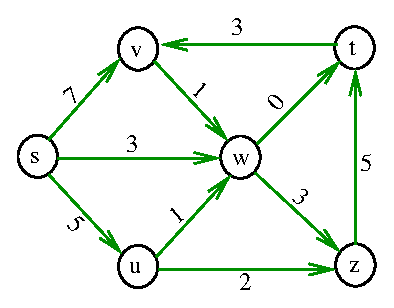
\includegraphics[scale=0.9]{./figs/caminho-custo2.eps}
  \quad \quad
  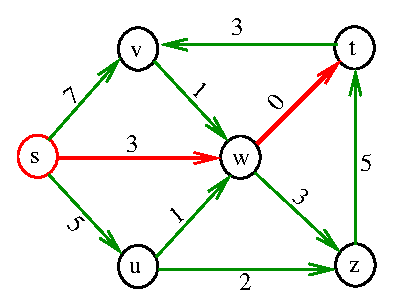
\includegraphics[scale=0.9]{./figs/caminho-custo3.eps}
 \caption{\label{fig:custo1} Um grafo com custos nos arcos. 
   O custo do caminho $\seq{s,u,w,z,t}$ � 14. � direita o  caminho de
custo m�nimo $\seq{s,w,t}$ est� em destaque.}
 \end{center}
\end{figure}

Como a nossa fun��o-custo � n�o-negativa, 
ent�o no grafo h� sempre um passeio de custo m�nimo que � uma caminho. 
Por esta raz�o, um passeio de custo m�nimo 
� simplesmente chamado de \defi{caminho m�nimo}\index{caminho!minimo@m�nimo}.



%Uma \defi{fun��o comprimento}\index{funcao@@fun��o!comprimento} %
%\index{comprimento!funcao@@fun��o} em
%$(V,A)$ � uma fun��o de $A$ em $\NonnegInt$. Se $c$ � uma fun��o
%comprimento em $(V,A)$ e $uv$ est� em $A$, ent�o, denotaremos por
%$c(u,v)$ o valor de $c$ em $uv$. 


Se $(V,A)$ � um grafo sim�trico e $c$ � 
uma fun��o comprimento em $(V,A)$, ent�o $c$ � 
\defi{sim�trica}\index{funcao@@fun��o!comprimento sim�trica} se
$c(uv) = c(vu)$ para todo arco $uv$. 
%%%% CZAO
O \defi{maior custo}\index{maior
  custo} de um arco ser� denotado por $C$\mar{$C$}, ou seja, 
$C := \max\{c(uv) \tq uv \in A \}$.
No grafo da figura~\ref{fig:custo1} temos que $C=7$.

%%% Comprimento de um passeio e passei de comprimento minimo.
%% Se $P$ � um passeio em um grafo $(V,A)$ e $c$ � uma fun��o comprimento, 
%% denotaremos por $c(P)$ o \defi{comprimento do caminho} $P$%
%% \index{comprimento!do caminho}, ou seja, $c(P)$ � o somat�rio dos comprimentos
%% de todos os arcos em $P$.  Um passeio $P$ tem \defi{comprimento m�nimo} se
%% $c(P) \leq c(P')$ para todo passeio $P'$ que tenha o mesmo in�cio e t�rmino
%% que $P$.  

A \defi{dist�ncia}\index{distancia@@dist�ncia} de um v�rtice $s$ a um
v�rtice $t$ � o menor custo de um caminho de $s$ a~$t$. 
A dist�ncia de $s$ a $t$ em rela��o a $c$ ser� denotada por 
$\distc{s,t}$\index{$\distc{s,t}$}\mar{$\distc{s,t}$}, ou simplesmente, 
quando a fun��o
custo estiver subentendida, por
$\dist{s,t}$\index{$\dist{s,t}$}\mar{$\dist{s,t}$}
denota a dist�ncia de $s$ a $t$. 
Na figura~\ref{fig:custo1} a dist�ncia de $s$ a $t$ � 4.
 


%%%%%%%%%%%%%%%%%%%%%%%%%%%%%%%%%%%%%%%%%%%%%%%%%%%%%%%%%%%%%%%%%%%%%%%%%%%%
%%
%%  DEFINI��O
%%
%%%%%%%%%%%%%%%%%%%%%%%%%%%%%%%%%%%%%%%%%%%%%%%%%%%%%%%%%%%%%%%%%%%%%%%%%%%% 
 
%\section{Defini��o do problema}
%
% Problema dos menores caminhos 
% 
 
Um problema fundamental em otimiza��o combinat�ria que tem um papel de
destaque nesta disserta��o � o 
\defi{problema do caminho m�nimo}, denotado por
\PCM:\index{problema!do caminho m�nimo@do caminho m�nimo}
 \begin{quote}
   \textbf{Problema} \PCM$(V,A,c,s,t)$: 
   \index{\PCM}\mar{\PCM}
%%%%%%%%%%%%%%%%%%%%%%%%%%%%%%%%%%%%%%%%%%%%%%%%%%%%%%%%%%%%%%%%%%%
   Dado um grafo $(V,A)$, uma fun��o
   custo~$c$ e dois v�rtice $s$ e $t$, 
   encontrar um caminho de custo m�nimo 
   de $s$ a~$t$.
 \end{quote}
Na literatura essa vers�o � conhecida como \textit{single-pair
  shortest path problem}\index{single-pair shortest path@single-source
  shortest path}.  O celebrado algoritmo de Edsger Wybe
Dijkstra~\cite{dijkstra59:note}, apresentado na
se��o~\ref{sec:dijkstra}, resolve o problema do caminho m�nimo.

 
%%%%%%%%%%%%%%%%%%%%%%%%%%%%%%%%%%%%%%%%%%%%%%%%%%%%%%%%%%%%%%%%%%%%%%%%%%%%
%%
%%  SE��O: FUN��ES POTENCIAL
%%
%%%%%%%%%%%%%%%%%%%%%%%%%%%%%%%%%%%%%%%%%%%%%%%%%%%%%%%%%%%%%%%%%%%%%%%%%%%% 
 
\section{Fun��es potenciais e crit�rio de otimalidade}
\label{sec:criterio-otimalidade}

Como � poss�vel provar que um dado caminho de um v�rtice 
$s$ a um v�rtice $t$ � de custo m�nimo?
Algoritmos para o \PCM{} fornecem certificados de otimalidade de 
suas respostas. Esses certificados v�m de dualidade de programa��o linear.
De fato, o seguinte programa linear, que chamamos de primal, � uma
relaxa��o do pro\-ble\-ma do caminho m�nimo: encontrar um vetor
$x$ indexado por $A$ que
\begin{eqnarray*}
\begin{array}{rrlrl}
\mbox{minimize} & cx \hfill\\
\mbox{sob as restri��es} & x(\sai(s)) - x(\entra(s)) \hfill & = & 1 \\
& x(\sai(t)) -  x(\entra(t)) \hfill & = & -1 \\
& x(\sai(v)) - x(\entra(v)) \hfill & = & 0 & \mbox{para cada $v$
em $V \setminus \{s,t\}$} \\
& x[uv] & \geq & 0 & \mbox{para cada $uv$ em $A$.}
\end{array}
\end{eqnarray*}

De fato, cada vetor caracter�stico de um caminho se $s$ a $t$ �
uma solu��o vi�vel do problema primal.

O respectivo problema dual consiste em encontrar um vetor $y$
indexado por $V$ que
\begin{eqnarray*}
\begin{array}{rllll}
\mbox{maximize} & y(t)-y(s) \\
\mbox{sob as restri��es} & y(v) -  y(u) & \leq & c(uv) &
\mbox{para cada $uv$ em $A$.}
\end{array}
\end{eqnarray*}



Se um v�rtice $t$ n�o
� acess�vel a partir de $s$ um algoritmo pode, para comprovar este fato,
devolver uma parte $S$ de $V$ tal que $s \in S$, $t \not\in S$ e n�o existe
$uv$ com $u$ em $S$ e $v$ em $V\setminus S$, ou seja $A(S)= \emptyset$. Este
seria um certificado combinat�ria de \defi{n�o-acessibilidade} de $t$ por $s$.
Entretanto, os certificados fornecidos pelos algoritmos, baseados em fun��es
potencial, ser�o um atestado compacto para certificar ambos: a otimalidade
dos caminhos fornecidos, e a n�o acessabilidade de alguns v�rtices por $s$.

Uma \defi{fun��o-potencial}\index{funcao@@fun��o!potencial}%
\index{potencial!funcao@@fun��o} � uma fun��o de $V$ em $\Int$.
Se $y$ � uma fun��o-potencial e $c$ � uma fun��o-custo, 
ent�o, dizemos que $y$ � um \defi{$c$-potencial}\index{c-potencial@$c$-potencial}
se 
 \begin{center}
   $y(v) - y(u) \leq c(uv)$ para cada arco $uv$ em $A$ (figura~\ref{fig:potencial}).
 \end{center}


\begin{figure}
\begin{center}
  \psfrag{0}{\red $1$}
  \psfrag{1}{\red $1$}
  \psfrag{2}{\red $1$}
  \psfrag{3}{\red $1$}
  \psfrag{4}{\red $2$}
  \psfrag{5}{\red $2$}
  \psfrag{6}{\red $6$}
  \psfrag{7}{\red $7$}
  \psfrag{s}{$\scor$}
  \psfrag{t}{$\tcor$}
  \psfrag{v}{$\black v$}
  \psfrag{u}{$\black u$}
  \psfrag{w}{$\black w$}
  \psfrag{z}{$\black z$}
  \psfrag{c}{$c$}
  \psfrag{ps}{\blue $2$}
  \psfrag{pt}{\blue $3$}
  \psfrag{pv}{\blue $4$}
  \psfrag{pu}{\blue $4$}
  \psfrag{pw}{\blue $3$}
  \psfrag{pz}{\blue $4$}
  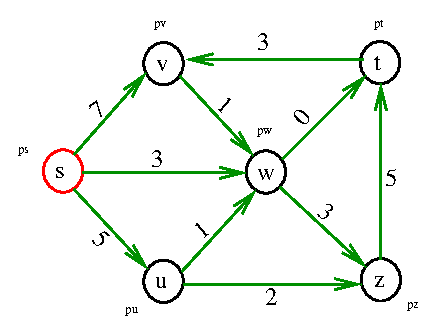
\includegraphics[scale=1]{./figs/c-potencial.eps}
\end{center}
\caption{\label{fig:potencial} (a) Um grafo com custos nos arcos. 
   e um c-potencial. Os n�meros pr�ximos aos v�rtices s�o os seu ponteciais.}
\end{figure}



%%%%%%%%%%%%%%%%%%%%%%%%%%%%%%%%%%%%%%%%%%%
%Se $y$ respeita $c$ em $A$ ent�o diz-se que $y$ � 
%\defi{vi�vel}\index{funcao@@fun��o!potencial viavel@@potencial vi�vel}. 
%%%%%%%%%%%%%%%%%%%%%%%%%%%%%%%%%%%%%%%%%%%%%%%%%

Limitantes inferiores para custo de
caminhos s�o obtidos atrav�s de $c$-potenciais. 
Este fato est� no lema a seguir, que 
� uma particulariza��o do conhecido lema da dualidade de 
programa��o linear~\cite{pf:proglin}.

%%%%%%%%%%%%%%%%%%%%%%%%%
%Suponha que $c$ � uma fun��o-custo em $(V,A)$ e que $P$ � um
%caminho de um v�rtice $s$ a um v�rtice $t$. Suponha ainda que $y$ � um
%$c$-potencial. Vale que
%\[
%c(P) \geq y(t) - y(s).
%\]
%%%%%%%%%%%%%%%%%%%%%%%%%%


\begin{lema}{lema da dualidade}\index{lema!da dualidade}\index{dualidade}
 \label{lema:dualidade}
  Seja $(V,A)$ um grafo e $c$ uma fun��o-custo sobre $V$. 
Para todo caminho $P$ com in�cio em $s$ e t�rmino em $t$ e todo $c$-potencial $y$ 
vale que 
\[
c(P) \geq y(t) - y(s). 
\]
\end{lema}

\begin{prova}
Suponha que $P$ � o caminho $\seq{s = v_{0}, \alpha_{1}, v_{1}, \ldots,
  \alpha_{k}, v_{k} = t }$. 
Temos que
\[
\begin{array}{ccl}
 c(P)& =    & c(\alpha_{1}) + \ldots + c (\alpha_{k})\\
     & \geq & (y(v_{1}) - y(v_{0})) + (y(v_{2}) - y(v_{1})) 
              + \ldots + (y(v_{k}) - y(v_{k-1}))\\
     & =    & y(v_{k}) - y(v_{0}) = y(t) - y(s).
\end{array}
\]
\end{prova}

% Se $y$ � uma fun��o-potencial al que $y(s) = 0$, ent�o para cada
% v�rtice $t$ o valor de $y(t)$ pode ser interpretada como uma dist�ncia
% tentativa de $s$ a $t$.


%%%%%%%%%%%%%%%%%%%%%%%%%%%%%%%%%%%%%%%%%%%%%%%%%%%%%%%%%%%%%%%%%%%%%%
% A seguir est�o dois corol�rios imediatos do lema da dualidade.
 
% Um conseq��ncia i
%  \begin{prova}

%  Seja $y$ uma fun��o-potencial vi�vel sobre $V$ e 

%  $P = \seq{s = v_{0}, \alpha_{1}, v_{1}, \ldots, \alpha_{k}, v_{k} = t }$ 
%  um caminho em $(V,A)$.

%  Tem-se que
% \[
% \begin{array}{ccl}
%  c(P)& =    & c_{\alpha_{1}} + \ldots + c_{\alpha_{k}}\\
%      & \geq & y(v_{1}) - y(v_{0}) + y(v_{2}) - y(v_{1}) 
%               + \ldots +y(v_{k}) - y(v_{k-1})\\
%      & =    & y(v_{k}) - y(v_{0}) = y(t) - y(s)
% \end{array}
% \]
% Portanto, $y(t) - y(s) \leq c(P)$.
% \end{prova}
% \end{lema}

 Do lema~\ref{lema:dualidade} tem-se imediatamente os seguintes corol�rios.

\begin{corolario}{condi��o de inacessabilidade}%
\index{condicao de@@condi��o de!inacessabilidade}\index{inacessabilidade}
\label{corolario:inacessabilidade}
Se $(V,A)$ � um grafo, $c$ � uma fun��o-custo, $y$ � um $c$-potencial
 e $s$ e $t$ s�o vertices tais que 
\[
y(t) - y(s) \geq nC + 1
\]
ent�o, $t$ n�o � acess�vel a partir de $s$
\fimprova
\end{corolario}


\begin{corolario}{condi��o de otimalidade}%
\index{condicao de@@condi��o de!otimalidade}\index{otimalidade}
\label{corolario:otimalidade}
Seja $(V,A)$ um grafo e $c$ � uma fun��o-custo.
Se $P$ � um caminho de $s$ a $t$ e $y$ � um $c$-potencial tais que 
$y(t) - y(s) = c(P)$, ent�o $P$ � um 
caminho que tem custo m�nimo.
\fimprova
\end{corolario}

\begin{figure}
\begin{center}
  \psfrag{0}{\red $1$}
  \psfrag{1}{\red $1$}
  \psfrag{2}{\red $2$}
  \psfrag{3}{\red $3$}
  \psfrag{4}{\red $4$}
  \psfrag{5}{\red $5$}
  \psfrag{6}{\red $6$}
  \psfrag{7}{\red $7$}
  \psfrag{s}{$\scor$}
  \psfrag{t}{$\tcor$}
  \psfrag{v}{\black $v$}
  \psfrag{u}{\black $u$}
  \psfrag{w}{\black $w$}
  \psfrag{z}{\black $z$}
  \psfrag{c}{$c$}
  \psfrag{ps}{\blue $0$}
  \psfrag{pt}{\blue $3$}
  \psfrag{pv}{\blue $5$}
  \psfrag{pu}{\blue $4$}
  \psfrag{pw}{\blue $3$}
  \psfrag{pz}{\blue $1$}
  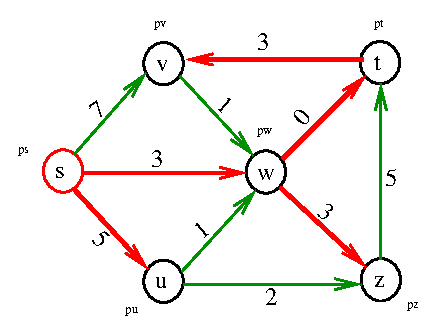
\includegraphics{./figs/potencial-otimo.eps}
\end{center}
\caption{\label{fig:potencial-otimo} Um grafo com custos nos arcos e um 
potencial que certifica que qualquer um dos caminhos com 
arcos em destaque t�m custo m�nimo.}
\end{figure}




%%%%%%%%%%%%%%%%%%%%%%%%%%%%%%%%%%%%%%%%%%%%%%%%%%%%%%%%%%%%%%%%%%%%%%%%%%%%
%%
%%  SE��O:  FUN��O-PREDECESSOR 
%%
%%%%%%%%%%%%%%%%%%%%%%%%%%%%%%%%%%%%%%%%%%%%%%%%%%%%%%%%%%%%%%%%%%%%%%%%%%%% 
 
\section{Representa��o de caminhos}
\label{sec:predecessor}

Uma maneira compacta de representar caminhos de dado v�rtice at� cada um dos
demais v�rtices de um grafo � atrav�s de uma fun��o-predecessor.
%%% FUN��O-PREDECESSOR 
Uma \defi{fun��o-pre\-de\-ces\-sor}
\index{funcao@@fun��o!predecessor}\index{predecessor!funcao@@fun��o} 
 � uma fun��o ``parcial'' 
$\pred$ de $V$ em $V$ tal que, para cada $v$ em $V\,$,
\[
\pred(v) = \nil \quad \mbox{ou} \quad (\pred(v),v) \in A
\] 


Se $(V,A)$ � um grafo, $\pred$ uma fun��o
predecessor sobre $V$ e $v_{0}, v_{1}, \ldots,v_{k}$ s�o v�rtices
tais que
\begin{enumerate}
\item[$\iten{1}$] $ v_{0} = \pred(v_{1}), v_{2} = \pred(v_{3}),
  \ldots, v_{k-1} = \pred(v_{k})$; e
          
\item[$\iten{2}$] $\alpha_{i} := v_{i-1}v_{i}$ est� em $A$ para $i =
  1, \ldots, k$.
\end{enumerate}
ent�o dizemos que $\seq{v_{0}, \alpha_{1}, v_{1}, \ldots, \alpha_{k},
v_{k}}$ � um \defi{caminho determinado por
$\pred$}\index{caminho!determinado por $\pred$}. 

Seja $\pred$ uma fun��o-predecessor e $\Psi := \{ uv \in A \tq u =
\pred(v)\}$. Dizemos em $(V,\Psi)$ � o \defi{grafo de
  predecessores}\index{grafo!predecessores}. 

%e que $\psi$
%\defi{determina uma
%  arboresc�ncia}\index{arborescencia@@arboresc�ncia!determinada por
%  $\pred$} quando o grafo $(V,\Psi)$ � uma arboresc�ncia.

Os algoritmos descritos nesta disserta��o utilizam fun��es predecessor para
compactamente representar todos os caminhos de custo m�nimo a partir
de um dado v�rtice. Conforme ilustrado na figura~\ref{fig:pred}.

\begin{figure}[htbp]
 \begin{center}
  \psfrag{0}{$ $}
  \psfrag{1}{$ $}
  \psfrag{2}{$ $}
  \psfrag{3}{$ $}
  \psfrag{4}{$ $}
  \psfrag{5}{$ $}
  \psfrag{6}{$ $}
  \psfrag{7}{$ $}
  \psfrag{8}{$ $}
  \psfrag{9}{$ $}
  \psfrag{s}{$\scor$}
  \psfrag{t}{$\tcor$}
  \psfrag{v}{$v$}
  \psfrag{u}{$u$}
  \psfrag{w}{$w$}
  \psfrag{z}{$z$}
  \psfrag{TABELA}{
    \begin{tabular}{c ^^7c c}
      v�rtice & $\pred$ \\ \hline
      $\scor$ & \scor  \\
      $w$      & $s$ \\
      $u$      & $s$ \\
      $\tcor$  & $w$ \\
      $z$      & $w$ \\
      $v$      & $t$ \\
    \end{tabular}
     }
  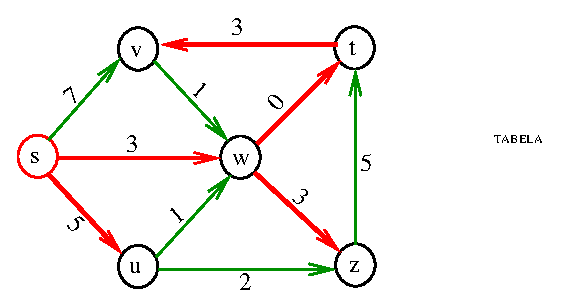
\includegraphics{./figs/caminho-custo4.eps}
  %\caption[{\sf Representa��o de caminhos atrav�s da fun��o-predecessor}]
  \caption[Representa��o de caminhos atrav�s da fun��o-predecessor]
  {\label{fig:pred} Representa��o de caminhos atrav�s da
    fun��o-predecessor $\pred$ com v�rtice inicial $\scor$. 
%Os   n�meros pr�ximo aos arcos representam o custo do arco. 
Os arcos
    em destaque formam uma arborec�ncia. A tabela ao lado mostra
    os valores de $\pred$.}
 \end{center}
 \end{figure}

  
%%%%%%%%%%%%%%%%%%%%%%%%%%%%%%%%%%%%%%%%%%%%%%%%%%%%%%%%%%%%%%%%%%%%%%%%%%%%
%%
%%  SE��O: EXAMINANDO UM V�RTICE
%%
%%%%%%%%%%%%%%%%%%%%%%%%%%%%%%%%%%%%%%%%%%%%%%%%%%%%%%%%%%%%%%%%%%%%%%%%%%%%
\section{Examinando arcos e v�rtices}
\label{sec:examinar}

%%%% Bl� inicial
Algoritmos para encontrar caminhos m�nimos mant�m, tipicamente, al�m de uma
fun��o-predecessor, uma fun��o-potencial. 
O valor desta fun��o-potencial para cada v�rtice � um limitante inferior para
o custo dos caminhos que tem como origem o v�rtice $s$, como mostra 
o lema da dualidade.  
Esta fun��o �
intuitivamente interpretada como uma \defi{dist�ncia
  tentativa}\index{distancia@@dist�ncia!tentativa} a  partir de $s$. 

%%% Examinar arco
Seja $y$ uma fun��o-potencial e $\pred$ uma fun��o-predecessor.
Uma opera��o b�sica envolvendo as fun��es $\pred$ e $y$ �
\defi{examinar um arco}\index{examinar um/uma!arco}
(\textit{relaxing}~\cite{clrs:introalg-2001},
 \textit{labeling step}~\cite{tarjan:data}). Examinar um arco $uv$ consiste em
 verificar se $y$ respeita  $c$ em $uv$ e, caso n�o respeite, ou seja,
\[
y(v) - y(u) > c(uv) \ \ \mbox{ou, equivalentemente} \ \ 
y(v) > y(u) + c(uv)
\]
fazer 
\[
y(v) \larr y(u) + c(uv) \ \ \mbox{e} \ \ \pred(v) \larr u.
\]
Intuitivamente, ao  examinar um arco $uv$ tenta-se encontrar um "atalho"
para o caminho de $s$ a $v$ no grafo de predecessores, passando por
$uv$.
O passo de examinar $uv$ pode diminuir o valor da dist�ncia
tentativa dos v�rtices $v$  e atualizar o predecessor, tamb�m tentativo,
de $v$ no caminho de custo m�nimo de $s$ a $v$. 



\begin{algoritmo}
\ExamineArco{} $(uv)$ \quad $\rhd$ examina o arco $uv$

1 \x \se{} $y(v) > y(u) + c(u,v)$ 


2 \xx \entao\ $y(v) \larr y(u) + c(uv)$ 

3 \xx \phentao{}  $\pred(v) \larr u$
%
%Para cada arco $uv$ tal que $d(v) > d(u) + c(u,v)$ fa�a \\
%\x $d(v) := d(u) + c(u,v)$ e $\pred(v) := u$. 
\end{algoritmo}


O consumo de tempo para examinar um arco � constante.


%%%% Examinar v�rtice
Outra opera��o b�sica � \defi{examinar um v�rtice}%
\index{examinar um/uma!vertice@@v�rtice}. 
Se $u$ � um examinar um consiste em examinar todos os arcos da forma $uv$. Em
linguagem algor�tmica tem-se
\begin{algoritmo}
\ExamineVertice{} $(u)$ \quad $\rhd$ examina o v�rtice $u$

1\x   \para{} \cada{} $uv$ em $A(u)$ \faca{}

2 \xx \ExamineArco{} $(uv)$
%
%Para cada arco $uv$ tal que $d(v) > d(u) + c(u,v)$ fa�a \\
%\x $d(v) := d(u) + c(u,v)$ e $\pred(v) := u$. 
\end{algoritmo}

ou ainda, de uma maneira expandida

\begin{algoritmo}
\ExamineVertice{} $(u)$ \quad $\rhd$ examina o v�rtice $u$

1\x   \para{} \cada{} $uv$ em $A(u)$ \faca{}

2 \xx \se{} $y(v) > y(u) + c(uv)$ 


3 \xxx \entao\ $y(v) \larr y(u) + c(uv)$ 

4 \xxx \phentao{}  $\pred(v) \larr u$
%
%Para cada arco $uv$ tal que $d(v) > d(u) + c(u,v)$ fa�a \\
%\x $d(v) := d(u) + c(u,v)$ e $\pred(v) := u$. 
\end{algoritmo}
O consumo de tempo para examinar um v�rtice � proporcional ao n�mero de arcos
com ponta inicial no v�rtice.

%%%%%%%%%%%%%%%%%%%%%%%%%%%%%%%%%%%%%%%%%%%%%%%%%%%%%%%%%%%%%%%%%%%%%%%%%%%%
%%
%%  SE��O: DIJKSTRA 
%%
%%%%%%%%%%%%%%%%%%%%%%%%%%%%%%%%%%%%%%%%%%%%%%%%%%%%%%%%%%%%%%%%%%%%%%%%%%%%
\section{Algoritmo de Dijsktra}
\label{sec:dijkstra}


Nesta se��o � descrito o celebrado algoritmo de
Edsger Wybe Dijkstra~\cite{dijkstra59:note} que resolve o problema do caminho m�nimo
%%%%%%%%%%%%%%%%%%%%%%%%%%%%%%%%%%%%%%%%%%%%%%%%%%%%%%%%%%%%%%%%%%%%%%%%%%%%%%%%%%
%% Para cada v�rtice de $t$ acess�vel a partir de um dado v�rtice $s$ o algoritmo
%% de Dijkstra encontra um caminho de $s$ a $t$ que tem custo m�nimo.  Da
%% condi��o de otimalidade (corol�rio~\ref{corolario:otimalidade}) tem-se que
%% para certificar que um caminho $P$ de $s$ a $t$ tem
%% custo m�nimo basta exibir um $c$-pontencial $y$ tal que $c(P)
%% = y(t) - y(s)$. Por outro lado, a condi��o de inacessabilidade
%% (corol�rio~\ref{corolario:inacessabilidade}) diz que se $y$ � um $c$-potencial
%% com $y(t) - y(s) = nC + 1$, ent�o $t$ n�o existe caminho de $s$ a $t$,
%% onde $n$ � o n�mero de v�rtices do grafo e $C := \max\{c(uv)
%% \tq uv \in A\}$. A corre��o do algoritmo de Dijkstra
%% fornecer� a rec�proca dessas condi��es.


A id�ia geral do algoritmo de Dijkstra para resolver o problema � a seguinte.
O algoritmo � iterativo.  No in�cio de cada itera��o tem-se uma parti��o $S$ e $Q$ 
dos  conjuntos vertices. O algoritmo conhece caminhos de $\scor$ a cada
v�rtice em $S$ e a uma parte dos v�rtices em $\Qcor$. Para os v�rtice em $S$ 
o caminho conhecido tem custo m�nimo. Cada itera��o consiste em remover um v�rtice
apropriado de $Q$, inclu�-lo $S$ e examin�-lo, atualizando, eventualmente,
o custo dos caminhos a alguns v�rtices em $Q$.


O algoritmo recebe um grafo $(V,A)$, uma fun��o-custo $c$ de $A$ 
em $\NonnegInt$ e um v�rtice~$s$ e devolve uma
fun��o-predecessor $\pred$ e uma fun��o-potencial~$y$ que respeita~$c$
tais que, para cada v�rtice $t$, se $t$ � acess�vel a partir de $s$, ent�o
$\pred$ determina um caminho de $s$ a $t$ que tem comprimento $y(t) - y(s)$, caso contr�rio $y(t)-y(s) = nC+1$, 
onde $C := \max\{ c(uv) \tq uv \in A\}.$
Da condi��o de otimalidade (corol�rio~\ref{corolario:otimalidade}) tem-se que
$\pred$ determina um caminho de $s$ a um v�rtice $t$, ent�o este caminho tem custo m�nimo.
Por outro lado, a condi��o de inacessabilidade
(corol�rio~\ref{corolario:inacessabilidade}) diz que se $y$ � um $c$-potencial
com $y(t) - y(s) = nC + 1$, ent�o n�o existe caminho de $s$ a $t$.
A corre��o do algoritmo de Dijkstra
fornecer� a rec�proca dessas condi��es.


A descri��o a seguir � a mesma das notas de aula de Feofiloff~\cite{pf:fluxos}.


\begin{algoritmo}
\Dijkstra{} $(V, A, c, \scor)$ \quad {$\rhd$  $c \geq 0$}

1\x \para{} \cada{} $v$ em $V$ \faca

2\xx    $y(v) \larr nC+1$ \quad {$\rhd$  $nC+1$ faz o papel de $\infty$} 

3\xx    $\pred(v) \larr \nil$

4\x  $y(\scor) \larr 0$

5\x $Q \larr N$  \quad {$\rhd$  $Q$ func. como uma fila com
  prioridades} 

6\x \enquanto{} $Q \neq \seq{}$ \faca

7\xx retire de $Q$ um v�rtice $u$ com $y(u)$ m�nimo

%\d7\xx escolha $\icor$ em $\Qcor$ de modo que $\ycor(\icor)$ seja m�nimo

%\d8\xx $\Qcor \larr \Qcor - \{\icor\}$ 

8\xx \ExamineVertice~$(u)$

%\d\ph{2}\xxxx {\gray $\rhd$ � poss�vel que $\jcor$ j� esteja em $\Qcor$}\\[2mm]
9\x \devolva{} $\pred$ e $y$
\end{algoritmo}


A vers�o mais expandida � 

\begin{algoritmo}
\Dijkstra{} $(V, A, c, \scor)$ \quad {$\rhd$  $c \geq 0$}

\d1\x \para{} \cada{} $v$ em $V$ \faca

\d2\xx    $y(v) \larr nC+1$ \quad {$\rhd$  $nC+1$ faz o papel de $\infty$} 

\d3\xx    $\pred(v) \larr \nil$

\d4\x  $y(\scor) \larr 0$

\d5\x $Q \larr N$  \quad {$\rhd$  $Q$ func. como uma fila com
  prioridades} 

\d6\x \enquanto{} $Q \neq \seq{}$ \faca

\d7\xx retire de $Q$ um v�rtice $u$ com $y(u)$ m�nimo

%\d7\xx escolha $\icor$ em $\Qcor$ de modo que $\ycor(\icor)$ seja m�nimo

%\d8\xx $\Qcor \larr \Qcor - \{\icor\}$ 

\d8\xx \para{} \cada{} $uv$ em $A(u)$ \faca{}

\d9\xxx \se{} $y(v) > y(u) + c(uv)$ \entao{}

10\xxxx $y(v) \larr y(u)+ c(uv) $

11\xxxx $\pred(v) \larr u$

%12\xxxx acrescente $\jcor$ a $\Qcor$ 

%\d\ph{2}\xxxx {\gray $\rhd$ � poss�vel que $\jcor$ j� esteja em $\Qcor$}\\[2mm]
12\x \devolva{} $\pred$ e $y$
\end{algoritmo}



\subsection*{Simula��o}

A seguir vemos ilustrada a simula��o do algoritmo para a chamada
\Dijkstra~$(s)$.  Na figura~(a) vemos o grafo $(V,A)$ dado, onde o n�mero em {\red vermelho} pr�ximo a cada arco indica o seu custo. Por exemplo, $c(tv) = 0$ e $c(sw) = 4$.
Nas ilustra��es os v�rtices com interior azul claro s�o aqueles que est�o em
$Q$. Assim, na figura~(b) vemos que todos os v�rtices foram inseridos em $Q$.
A fun��o-potencial $y$ � indicada pelos n�meros em {\blue azul} 
pr�ximos cada v�rtice. Assim, na figura~(b), vemos que $y(\scor)=0$ 
e o potencial dos demais v�rtices � 
$n \times C + 1 = 6 \times 7 + 1 = 43$.

Durante a simula��o, o v�rtice sendo examinado t�m a cor rosa no seu
interior, enquanto o arco sendo examinado � mais espesso e tem a cor
azul.  Por exemplo, na figura~(c) o v�rtice sendo examinado � $\scor$ e
o arco sendo examinado � $\scor v$.

Os v�rtices que j� foram examinados e, portanto est�o em $S$ t�m a cor
verde em seu interior. Na figura~(j) vemos que $w$ est� sendo examinado, $\scor$ e $u$ s�o os v�rtices em $S$ e os demais est�o em $\Qcor$.


Os arcos j� examinados s�o espessos e t�m a cor vermelha ou s�o finos e
t�m a cor azul escura. Na figura~(k) vemos que o arco $wz$ est� sendo
examinado e os arcos j� examinados s�o $\scor v$, $\scor w$, $\scor u$, $u w$, $u z$  
e $wt$.

Os arcos em vermelho s�o os que formam o grafo de predecessores
com raiz $\scor$. Na figura~(k) os arcos do grafo de predecessores s�o 
$\scor v$, $\scor u$, $u w$, e  $wt$.
 
\begin{center}
  \psfrag{0}{\red $0$}
  \psfrag{1}{\red $7$}
  \psfrag{2}{\red $4$}
  \psfrag{3}{\red $2$}
  \psfrag{4}{\red $0$}
  \psfrag{5}{\red $1$}
  \psfrag{6}{\red $1$}
  \psfrag{7}{\red $3$}
  \psfrag{8}{\red $4$}
  \psfrag{9}{\red $1$}
  \psfrag{10}{\red $2$}
  \psfrag{s}{$\scor$}
  \psfrag{t}{$\tcor$}
  \psfrag{v}{\black $v$}
  \psfrag{u}{\black $u$}
  \psfrag{w}{\black $w$}
  \psfrag{z}{\black $z$}
  \psfrag{ps}{\blue $ $}
  \psfrag{pt}{\blue $ $}
  \psfrag{pv}{\blue $ $}
  \psfrag{pu}{\blue $ $}
  \psfrag{pw}{\blue $ $}
  \psfrag{pz}{\blue $ $}
  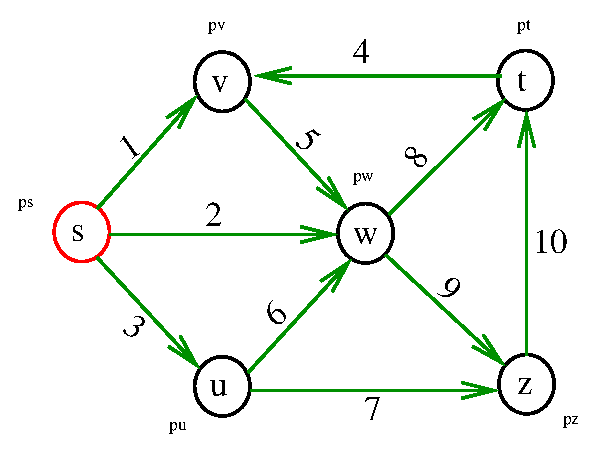
\includegraphics[scale=0.65]{./figs/dijkstra01.eps}
  \quad\quad
  \psfrag{0}{\red $0$}
  \psfrag{1}{\red $7$}
  \psfrag{2}{\red $4$}
  \psfrag{3}{\red $2$}
  \psfrag{4}{\red $0$}
  \psfrag{5}{\red $1$}
  \psfrag{6}{\red $1$}
  \psfrag{7}{\red $3$}
  \psfrag{8}{\red $4$}
  \psfrag{9}{\red $1$}
  \psfrag{10}{\red $2$}
  \psfrag{s}{$\scor$}
  \psfrag{t}{$\tcor$}
  \psfrag{v}{\black $v$}
  \psfrag{u}{\black $u$}
  \psfrag{w}{\black $w$}
  \psfrag{z}{\black $z$}
  \psfrag{ps}{\blue $0$}
  \psfrag{pt}{\blue $43$}
  \psfrag{pv}{\blue $43$}
  \psfrag{pu}{\blue $43$}
  \psfrag{pw}{\blue $43$}
  \psfrag{pz}{\blue $43$}
  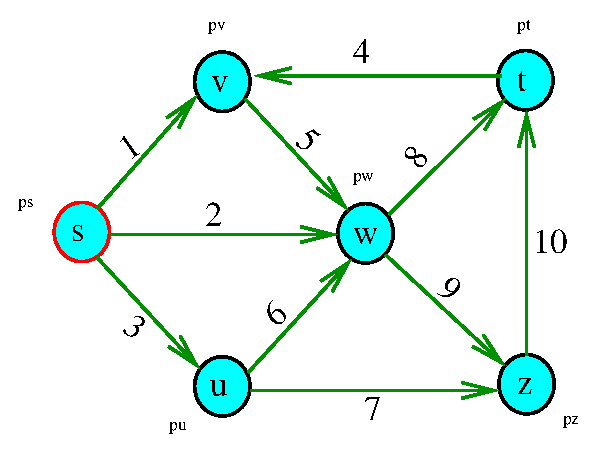
\includegraphics[scale=0.65]{./figs/dijkstra02.eps}

  \vspace*{-3mm}
  \hspace*{1cm}(a)\hspace*{7cm}(b) 
%\end{center}
%\begin{center}

  \psfrag{0}{\red $0$}
  \psfrag{1}{\red $7$}
  \psfrag{2}{\red $4$}
  \psfrag{3}{\red $2$}
  \psfrag{4}{\red $0$}
  \psfrag{5}{\red $1$}
  \psfrag{6}{\red $1$}
  \psfrag{7}{\red $3$}
  \psfrag{8}{\red $4$}
  \psfrag{9}{\red $1$}
  \psfrag{10}{\red $2$}
  \psfrag{s}{$\scor$}
  \psfrag{t}{$\tcor$}
  \psfrag{v}{\black $v$}
  \psfrag{u}{\black $u$}
  \psfrag{w}{\black $w$}
  \psfrag{z}{\black $z$}
  \psfrag{ps}{\blue $0$}
  \psfrag{pt}{\blue $43$}
  \psfrag{pv}{\blue $43$}
  \psfrag{pu}{\blue $43$}
  \psfrag{pw}{\blue $43$}
  \psfrag{pz}{\blue $43$}
  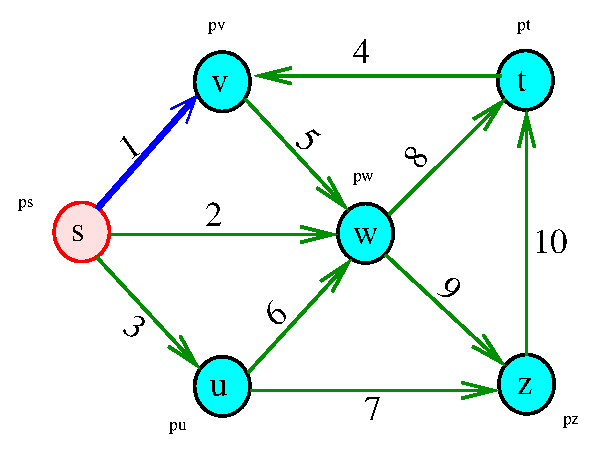
\includegraphics[scale=0.65]{./figs/dijkstra03.eps}
  \quad\quad
  \psfrag{0}{\red $0$}
  \psfrag{1}{\red $7$}
  \psfrag{2}{\red $4$}
  \psfrag{3}{\red $2$}
  \psfrag{4}{\red $0$}
  \psfrag{5}{\red $1$}
  \psfrag{6}{\red $1$}
  \psfrag{7}{\red $3$}
  \psfrag{8}{\red $4$}
  \psfrag{9}{\red $1$}
  \psfrag{10}{\red $2$}
  \psfrag{s}{$\scor$}
  \psfrag{t}{$\tcor$}
  \psfrag{v}{\black $v$}
  \psfrag{u}{\black $u$}
  \psfrag{w}{\black $w$}
  \psfrag{z}{\black $z$}
  \psfrag{ps}{\blue $0$}
  \psfrag{pt}{\blue $43$}
  \psfrag{pv}{\blue $7$}
  \psfrag{pu}{\blue $43$}
  \psfrag{pw}{\blue $43$}
  \psfrag{pz}{\blue $43$}
  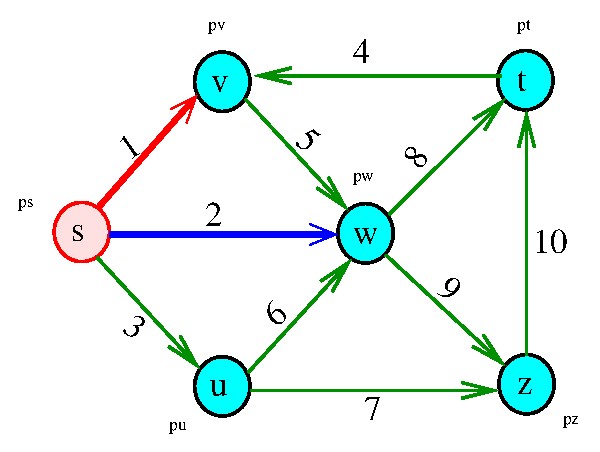
\includegraphics[scale=0.65]{./figs/dijkstra04.eps}

  \vspace*{-3mm}
  \hspace*{1cm}(c)\hspace*{7cm}(d)

%\end{center}
%\begin{center}

  \psfrag{0}{\red $0$}
  \psfrag{1}{\red $7$}
  \psfrag{2}{\red $4$}
  \psfrag{3}{\red $2$}
  \psfrag{4}{\red $0$}
  \psfrag{5}{\red $1$}
  \psfrag{6}{\red $1$}
  \psfrag{7}{\red $3$}
  \psfrag{8}{\red $4$}
  \psfrag{9}{\red $1$}
  \psfrag{10}{\red $2$}
  \psfrag{s}{$\scor$}
  \psfrag{t}{$\tcor$}
  \psfrag{v}{\black $v$}
  \psfrag{u}{\black $u$}
  \psfrag{w}{\black $w$}
  \psfrag{z}{\black $z$}
  \psfrag{ps}{\blue $0$}
  \psfrag{pt}{\blue $43$}
  \psfrag{pv}{\blue $7$}
  \psfrag{pu}{\blue $43$}
  \psfrag{pw}{\blue $4$}
  \psfrag{pz}{\blue $43$}
  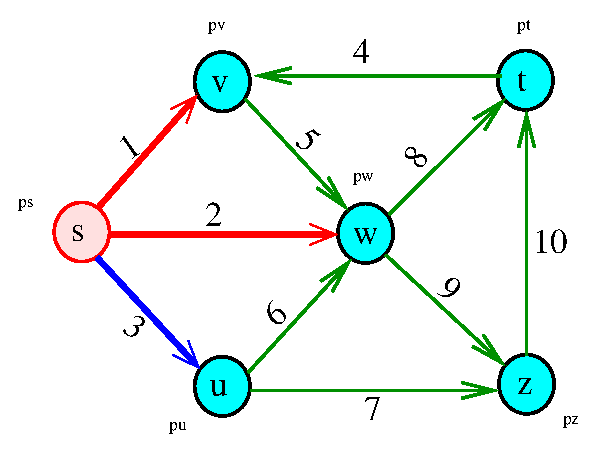
\includegraphics[scale=0.65]{./figs/dijkstra05.eps}
  \quad\quad
  \psfrag{0}{\red $0$}
  \psfrag{1}{\red $7$}
  \psfrag{2}{\red $4$}
  \psfrag{3}{\red $2$}
  \psfrag{4}{\red $0$}
  \psfrag{5}{\red $1$}
  \psfrag{6}{\red $1$}
  \psfrag{7}{\red $3$}
  \psfrag{8}{\red $4$}
  \psfrag{9}{\red $1$}
  \psfrag{10}{\red $2$}
  \psfrag{s}{$\scor$}
  \psfrag{t}{$\tcor$}
  \psfrag{v}{\black $v$}
  \psfrag{u}{\black $u$}
  \psfrag{w}{\black $w$}
  \psfrag{z}{\black $z$}
  \psfrag{ps}{\blue $0$}
  \psfrag{pt}{\blue $43$}
  \psfrag{pv}{\blue $7$}
  \psfrag{pu}{\blue $2$}
  \psfrag{pw}{\blue $4$}
  \psfrag{pz}{\blue $43$}
  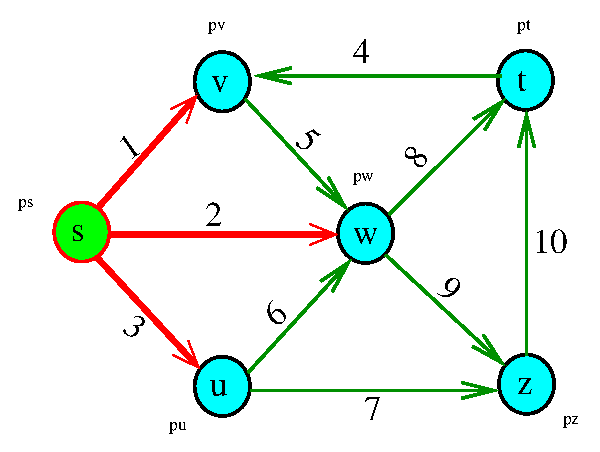
\includegraphics[scale=0.65]{./figs/dijkstra06.eps}

  \vspace*{-3mm}
  \hspace*{1cm}(e)\hspace*{7cm}(f)

%\end{center}
%\begin{center}

  \psfrag{0}{\red $0$}
  \psfrag{1}{\red $7$}
  \psfrag{2}{\red $4$}
  \psfrag{3}{\red $2$}
  \psfrag{4}{\red $0$}
  \psfrag{5}{\red $1$}
  \psfrag{6}{\red $1$}
  \psfrag{7}{\red $3$}
  \psfrag{8}{\red $4$}
  \psfrag{9}{\red $1$}
  \psfrag{10}{\red $2$}
  \psfrag{s}{$\scor$}
  \psfrag{t}{$\tcor$}
  \psfrag{v}{\black $v$}
  \psfrag{u}{\black $u$}
  \psfrag{w}{\black $w$}
  \psfrag{z}{\black $z$}
  \psfrag{ps}{\blue $0$}
  \psfrag{pt}{\blue $43$}
  \psfrag{pv}{\blue $7$}
  \psfrag{pu}{\blue $2$}
  \psfrag{pw}{\blue $4$}
  \psfrag{pz}{\blue $43$}
  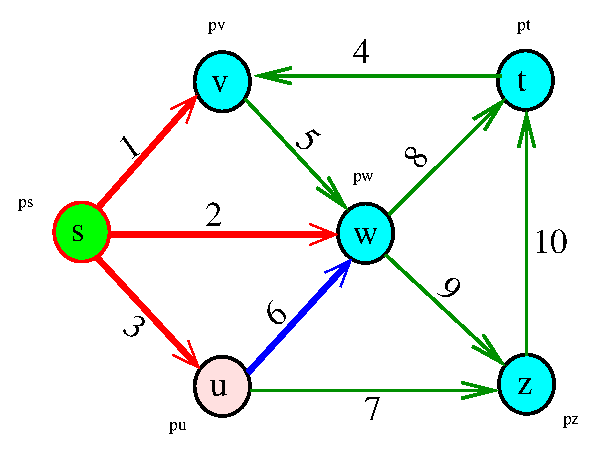
\includegraphics[scale=0.65]{./figs/dijkstra07.eps}
  \quad\quad
  \psfrag{0}{\red $0$}
  \psfrag{1}{\red $7$}
  \psfrag{2}{\red $4$}
  \psfrag{3}{\red $2$}
  \psfrag{4}{\red $0$}
  \psfrag{5}{\red $1$}
  \psfrag{6}{\red $1$}
  \psfrag{7}{\red $3$}
  \psfrag{8}{\red $4$}
  \psfrag{9}{\red $1$}
  \psfrag{10}{\red $2$}
  \psfrag{s}{$\scor$}
  \psfrag{t}{$\tcor$}
  \psfrag{v}{\black $v$}
  \psfrag{u}{\black $u$}
  \psfrag{w}{\black $w$}
  \psfrag{z}{\black $z$}
  \psfrag{ps}{\blue $0$}
  \psfrag{pt}{\blue $43$}
  \psfrag{pv}{\blue $7$}
  \psfrag{pu}{\blue $2$}
  \psfrag{pw}{\blue $3$}
  \psfrag{pz}{\blue $43$}
  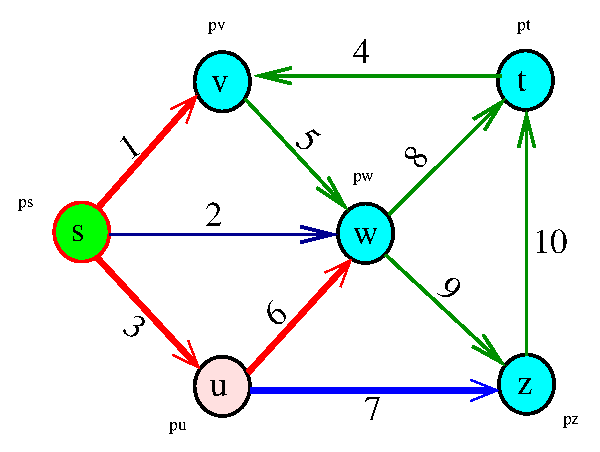
\includegraphics[scale=0.65]{./figs/dijkstra08.eps}

  \vspace*{-3mm}
  \hspace*{1cm}(g)\hspace*{7cm}(h)

%\end{center}
%\begin{center}

  \psfrag{0}{\red $0$}
  \psfrag{1}{\red $7$}
  \psfrag{2}{\red $4$}
  \psfrag{3}{\red $2$}
  \psfrag{4}{\red $0$}
  \psfrag{5}{\red $1$}
  \psfrag{6}{\red $1$}
  \psfrag{7}{\red $3$}
  \psfrag{8}{\red $4$}
  \psfrag{9}{\red $1$}
  \psfrag{10}{\red $2$}
  \psfrag{s}{$\scor$}
  \psfrag{t}{$\tcor$}
  \psfrag{v}{\black $v$}
  \psfrag{u}{\black $u$}
  \psfrag{w}{\black $w$}
  \psfrag{z}{\black $z$}
  \psfrag{ps}{\blue $0$}
  \psfrag{pt}{\blue $43$}
  \psfrag{pv}{\blue $7$}
  \psfrag{pu}{\blue $2$}
  \psfrag{pw}{\blue $3$}
  \psfrag{pz}{\blue $5$}
  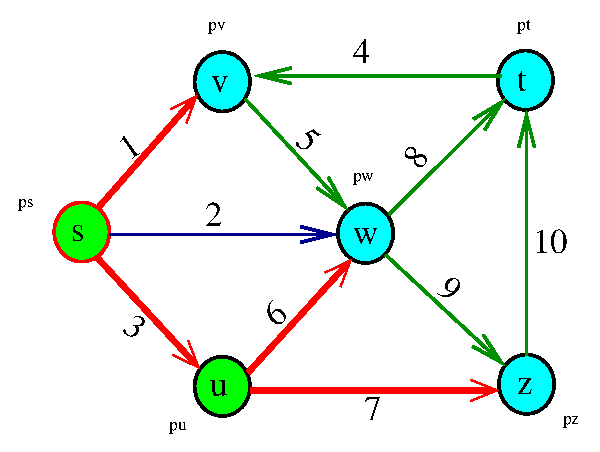
\includegraphics[scale=0.65]{./figs/dijkstra09.eps}
  \quad\quad
  \psfrag{0}{\red $0$}
  \psfrag{1}{\red $7$}
  \psfrag{2}{\red $4$}
  \psfrag{3}{\red $2$}
  \psfrag{4}{\red $0$}
  \psfrag{5}{\red $1$}
  \psfrag{6}{\red $1$}
  \psfrag{7}{\red $3$}
  \psfrag{8}{\red $4$}
  \psfrag{9}{\red $1$}
  \psfrag{10}{\red $2$}
  \psfrag{s}{$\scor$}
  \psfrag{t}{$\tcor$}
  \psfrag{v}{\black $v$}
  \psfrag{u}{\black $u$}
  \psfrag{w}{\black $w$}
  \psfrag{z}{\black $z$}
  \psfrag{ps}{\blue $0$}
  \psfrag{pt}{\blue $43$}
  \psfrag{pv}{\blue $7$}
  \psfrag{pu}{\blue $2$}
  \psfrag{pw}{\blue $3$}
  \psfrag{pz}{\blue $5$}
  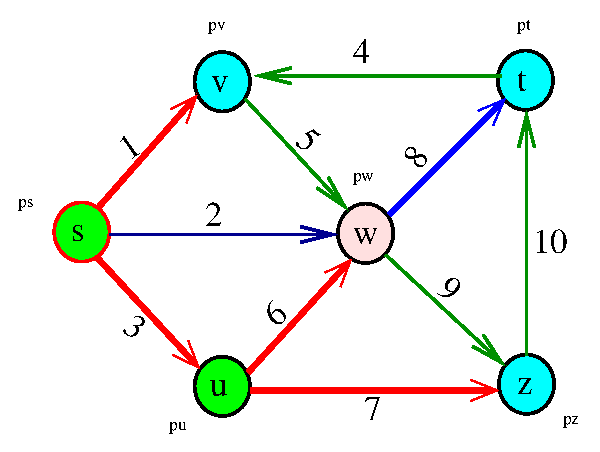
\includegraphics[scale=0.65]{./figs/dijkstra10.eps}

  \vspace*{-3mm}
  \hspace*{1cm}(i)\hspace*{7cm}(j)

%\end{center}
%\begin{center}

  \psfrag{0}{\red $0$}
  \psfrag{1}{\red $7$}
  \psfrag{2}{\red $4$}
  \psfrag{3}{\red $2$}
  \psfrag{4}{\red $0$}
  \psfrag{5}{\red $1$}
  \psfrag{6}{\red $1$}
  \psfrag{7}{\red $3$}
  \psfrag{8}{\red $4$}
  \psfrag{9}{\red $1$}
  \psfrag{10}{\red $2$}
  \psfrag{s}{$\scor$}
  \psfrag{t}{$\tcor$}
  \psfrag{v}{\black $v$}
  \psfrag{u}{\black $u$}
  \psfrag{w}{\black $w$}
  \psfrag{z}{\black $z$}
  \psfrag{ps}{\blue $0$}
  \psfrag{pt}{\blue $7$}
  \psfrag{pv}{\blue $7$}
  \psfrag{pu}{\blue $2$}
  \psfrag{pw}{\blue $3$}
  \psfrag{pz}{\blue $5$}
  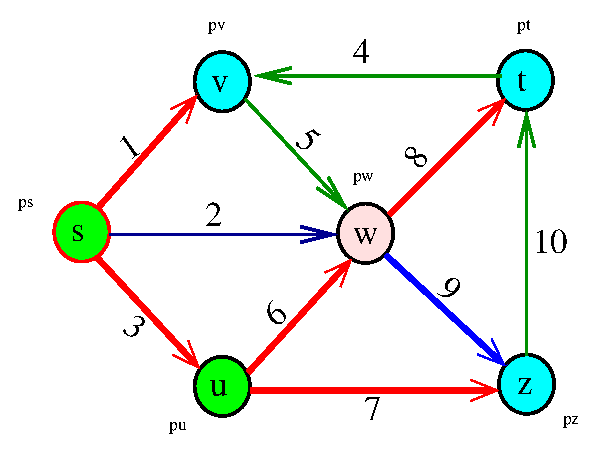
\includegraphics[scale=0.65]{./figs/dijkstra11.eps}
  \quad\quad
  \psfrag{0}{\red $0$}
  \psfrag{1}{\red $7$}
  \psfrag{2}{\red $4$}
  \psfrag{3}{\red $2$}
  \psfrag{4}{\red $0$}
  \psfrag{5}{\red $1$}
  \psfrag{6}{\red $1$}
  \psfrag{7}{\red $3$}
  \psfrag{8}{\red $4$}
  \psfrag{9}{\red $1$}
  \psfrag{10}{\red $2$}
  \psfrag{s}{$\scor$}
  \psfrag{t}{$\tcor$}
  \psfrag{v}{\black $v$}
  \psfrag{u}{\black $u$}
  \psfrag{w}{\black $w$}
  \psfrag{z}{\black $z$}
  \psfrag{ps}{\blue $0$}
  \psfrag{pt}{\blue $7$}
  \psfrag{pv}{\blue $7$}
  \psfrag{pu}{\blue $2$}
  \psfrag{pw}{\blue $3$}
  \psfrag{pz}{\blue $4$}
  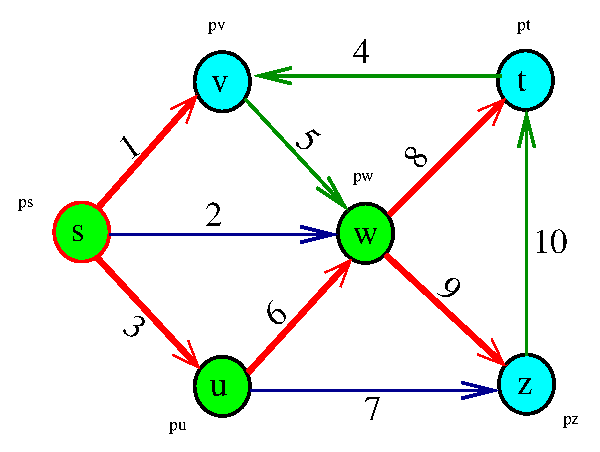
\includegraphics[scale=0.65]{./figs/dijkstra12.eps}

 \vspace*{-3mm}
  \hspace*{1cm}(k)\hspace*{7cm}(l)

%\end{center}
%\begin{center}

  \psfrag{0}{\red $0$}
  \psfrag{1}{\red $7$}
  \psfrag{2}{\red $4$}
  \psfrag{3}{\red $2$}
  \psfrag{4}{\red $0$}
  \psfrag{5}{\red $1$}
  \psfrag{6}{\red $1$}
  \psfrag{7}{\red $3$}
  \psfrag{8}{\red $4$}
  \psfrag{9}{\red $1$}
  \psfrag{10}{\red $2$}
  \psfrag{s}{$\scor$}
  \psfrag{t}{$\tcor$}
  \psfrag{v}{\black $v$}
  \psfrag{u}{\black $u$}
  \psfrag{w}{\black $w$}
  \psfrag{z}{\black $z$}
  \psfrag{ps}{\blue $0$}
  \psfrag{pt}{\blue $7$}
  \psfrag{pv}{\blue $7$}
  \psfrag{pu}{\blue $2$}
  \psfrag{pw}{\blue $3$}
  \psfrag{pz}{\blue $4$}
  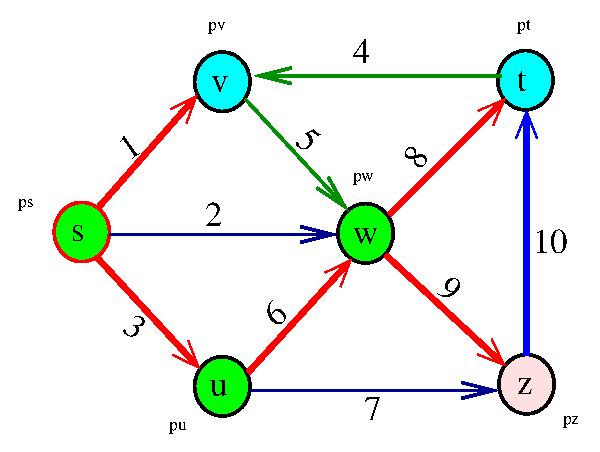
\includegraphics[scale=0.65]{./figs/dijkstra13.eps}
  \quad\quad
  \psfrag{0}{\red $0$}
  \psfrag{1}{\red $7$}
  \psfrag{2}{\red $4$}
  \psfrag{3}{\red $2$}
  \psfrag{4}{\red $0$}
  \psfrag{5}{\red $1$}
  \psfrag{6}{\red $1$}
  \psfrag{7}{\red $3$}
  \psfrag{8}{\red $4$}
  \psfrag{9}{\red $1$}
  \psfrag{10}{\red $2$}
  \psfrag{s}{$\scor$}
  \psfrag{t}{$\tcor$}
  \psfrag{v}{\black $v$}
  \psfrag{u}{\black $u$}
  \psfrag{w}{\black $w$}
  \psfrag{z}{\black $z$}
  \psfrag{ps}{\blue $0$}
  \psfrag{pt}{\blue $6$}
  \psfrag{pv}{\blue $7$}
  \psfrag{pu}{\blue $2$}
  \psfrag{pw}{\blue $3$}
  \psfrag{pz}{\blue $4$}
  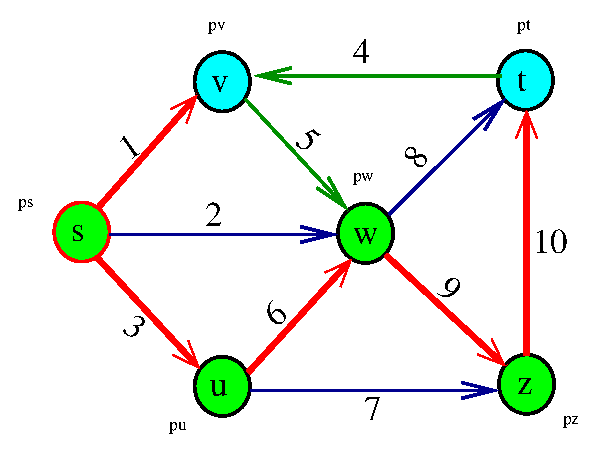
\includegraphics[scale=0.65]{./figs/dijkstra14.eps}

  \vspace*{-3mm}
  \hspace*{1cm}(m)\hspace*{7cm}(n)

%\end{center}
%\begin{center}

  \psfrag{0}{\red $0$}
  \psfrag{1}{\red $7$}
  \psfrag{2}{\red $4$}
  \psfrag{3}{\red $2$}
  \psfrag{4}{\red $0$}
  \psfrag{5}{\red $1$}
  \psfrag{6}{\red $1$}
  \psfrag{7}{\red $3$}
  \psfrag{8}{\red $4$}
  \psfrag{9}{\red $1$}
  \psfrag{10}{\red $2$}
  \psfrag{s}{$\scor$}
  \psfrag{t}{$\tcor$}
  \psfrag{v}{\black $v$}
  \psfrag{u}{\black $u$}
  \psfrag{w}{\black $w$}
  \psfrag{z}{\black $z$}
  \psfrag{ps}{\blue $0$}
  \psfrag{pt}{\blue $6$}
  \psfrag{pv}{\blue $7$}
  \psfrag{pu}{\blue $2$}
  \psfrag{pw}{\blue $3$}
  \psfrag{pz}{\blue $4$}
  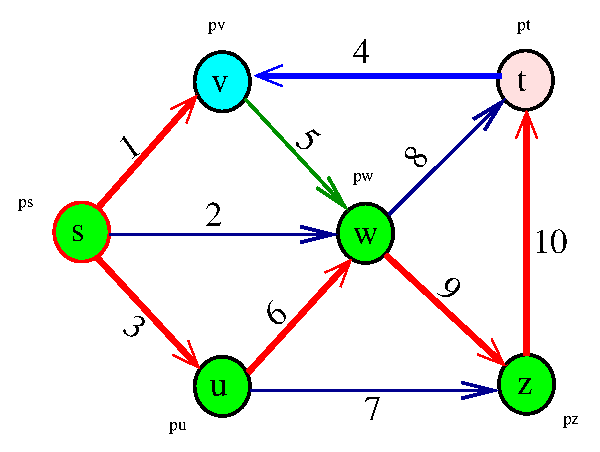
\includegraphics[scale=0.65]{./figs/dijkstra15.eps}
  \quad\quad
  \psfrag{0}{\red $0$}
  \psfrag{1}{\red $7$}
  \psfrag{2}{\red $4$}
  \psfrag{3}{\red $2$}
  \psfrag{4}{\red $0$}
  \psfrag{5}{\red $1$}
  \psfrag{6}{\red $1$}
  \psfrag{7}{\red $3$}
  \psfrag{8}{\red $4$}
  \psfrag{9}{\red $1$}
  \psfrag{10}{\red $2$}
  \psfrag{s}{$\scor$}
  \psfrag{t}{$\tcor$}
  \psfrag{v}{\black $v$}
  \psfrag{u}{\black $u$}
  \psfrag{w}{\black $w$}
  \psfrag{z}{\black $z$}
  \psfrag{ps}{\blue $0$}
  \psfrag{pt}{\blue $6$}
  \psfrag{pv}{\blue $6$}
  \psfrag{pu}{\blue $2$}
  \psfrag{pw}{\blue $3$}
  \psfrag{pz}{\blue $4$}
  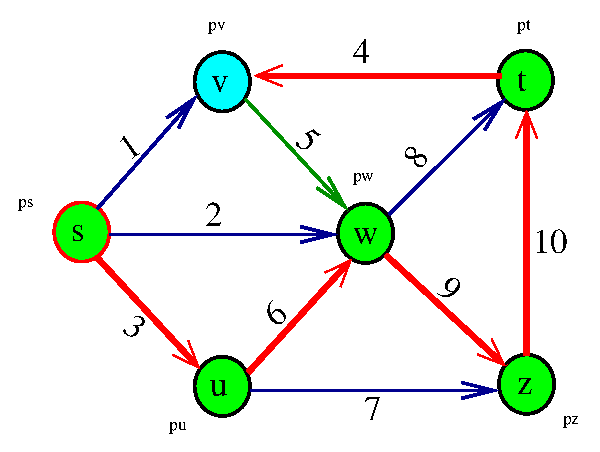
\includegraphics[scale=0.65]{./figs/dijkstra16.eps}

  \vspace*{-3mm}
  \hspace*{1cm}(o)\hspace*{7cm}(p)

%\end{center}
%\begin{center}

  \psfrag{0}{\red $0$}
  \psfrag{1}{\red $7$}
  \psfrag{2}{\red $4$}
  \psfrag{3}{\red $2$}
  \psfrag{4}{\red $0$}
  \psfrag{5}{\red $1$}
  \psfrag{6}{\red $1$}
  \psfrag{7}{\red $3$}
  \psfrag{8}{\red $4$}
  \psfrag{9}{\red $1$}
  \psfrag{10}{\red $2$}
  \psfrag{s}{$\scor$}
  \psfrag{t}{$\tcor$}
  \psfrag{v}{\black $v$}
  \psfrag{u}{\black $u$}
  \psfrag{w}{\black $w$}
  \psfrag{z}{\black $z$}
  \psfrag{ps}{\blue $0$}
  \psfrag{pt}{\blue $6$}
  \psfrag{pv}{\blue $6$}
  \psfrag{pu}{\blue $2$}
  \psfrag{pw}{\blue $3$}
  \psfrag{pz}{\blue $4$}
  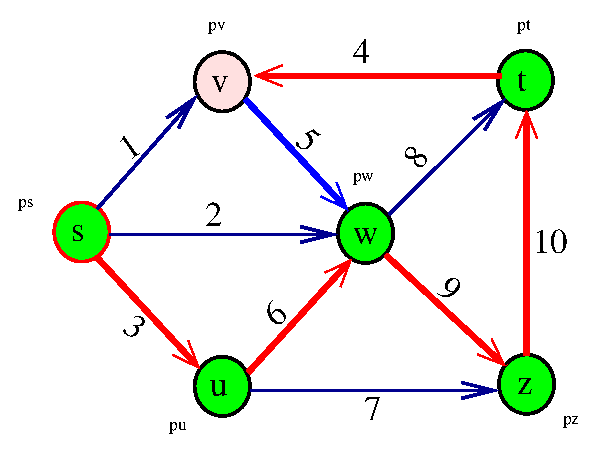
\includegraphics[scale=0.65]{./figs/dijkstra17.eps}
  \quad\quad
  \psfrag{0}{\red $0$}
  \psfrag{1}{\red $7$}
  \psfrag{2}{\red $4$}
  \psfrag{3}{\red $2$}
  \psfrag{4}{\red $0$}
  \psfrag{5}{\red $1$}
  \psfrag{6}{\red $1$}
  \psfrag{7}{\red $3$}
  \psfrag{8}{\red $4$}
  \psfrag{9}{\red $1$}
  \psfrag{10}{\red $2$}
  \psfrag{s}{$\scor$}
  \psfrag{t}{$\tcor$}
  \psfrag{v}{\black $v$}
  \psfrag{u}{\black $u$}
  \psfrag{w}{\black $w$}
  \psfrag{z}{\black $z$}
  \psfrag{ps}{\blue $0$}
  \psfrag{pt}{\blue $6$}
  \psfrag{pv}{\blue $6$}
  \psfrag{pu}{\blue $2$}
  \psfrag{pw}{\blue $3$}
  \psfrag{pz}{\blue $4$}
  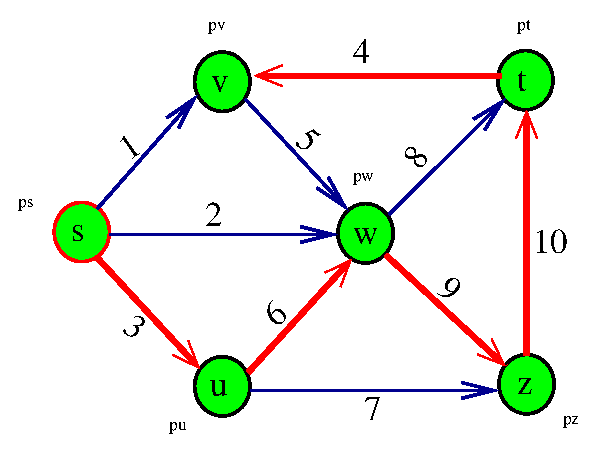
\includegraphics[scale=0.65]{./figs/dijkstra18.eps}

  \vspace*{-3mm}
  \hspace*{1cm}(q)\hspace*{7cm}(r)
\end{center}





\subsection*{Corre��o}


A corre��o do algoritmo de Dijkstra baseia-se nas demonstra��es da validade de
uma s�rie de rela��es invariantes, enunciadas a seguir. 
Estas rela��es s�o
afirma��es envolvendo os dados do problema $V,A,c$ e $s$ e os objetos $y,
\pred, S$ e $Q$. As afirma��es s�o v�lidas no in�cio de cada itera��o do
algoritmo e dizem como estes objetos se relacionam entre si e com os dados do
problema.


Na linha~6, antes da verifica��o da condi��o  ``$Q \neq \seq{}$'' 
valem as seguintes invariantes:
\begin{enumerate}
\item[(dk0)] para cada arco $pq$ no {\red grafo de
    predecessores} tem-se $y(q) - y(p) = c(pq)$;

\item[(dk1)] $\pred(s) = \nil$ e $y(s) = 0$;

\item[(dk2)] para cada v�rtice $v$ distinto de $s$,
$
yr(v) < n C+1 \Leftrightarrow  pi(v) \neq \nil;
$ 

\item[(dk3)] para cada v�rtice $v$, se $\pred(v) \neq \nil$ ent�o 
{\red existe} um caminho de $s$ a $v$ no {\red grafo de predecessores}.

\item[(dk4)] para cada arco $pq$ com $y(q) -
  y(p) > c(pq)$ tem-se que $p$~e $q$
  est�o~$Q$;

\item[(dk5)] ({\red monotonicidade}) para quaisquer $u$ em $V - Q$,   $v$ em $Q$ vale que
$$y(u) \leq y(v).$$ 
\end{enumerate}



\begin{figure}[htbp]
\begin{center}
  \psfrag{s}{\large $\scor$}
  \psfrag{S}{\large $S$}
  \psfrag{v}{\large $u$}
  \psfrag{Q}{\large $Q$}
  \psfrag{U}{\large $Q$}


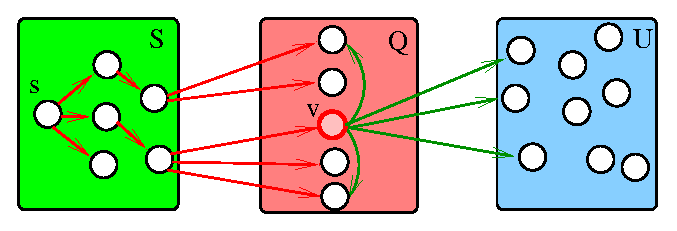
\includegraphics[scale=1.2]{./figs/iteracao.eps}


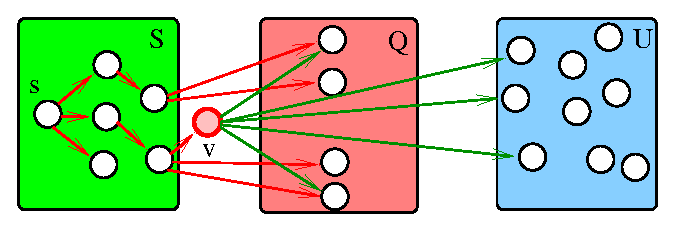
\includegraphics[scale=1.2]{./figs/iteracao1.eps}


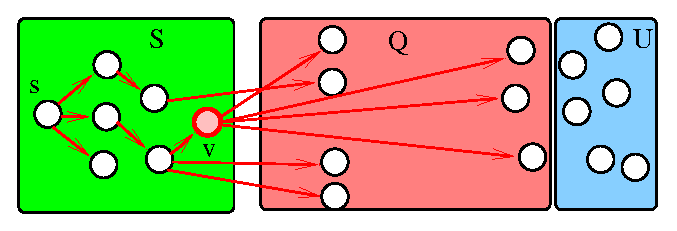
\includegraphics[scale=1.2]{./figs/iteracao2.eps}
%  \caption[{\sf Ilustra��o de uma itera��o de \Dijkstra}]
    \caption[Ilustra��o de uma itera��o de \Dijkstra]
  {\label{fig:iteracao} Ilustra��o de uma itera��o do algoritmo \Dijkstra.
    O arcos em vermelho formam o grafo de predecessores. }
\end{center}
\end{figure}

%\item[{\verde (i5)}] se $\Lcor = \seq{\icor_1, \icor_2, \ldots, \icor_{\lcor}}$ est�o
%\[
%\ycor(\icor_1) \leq \ycor(\icor_2) \leq \cdots \leq \ycor(\icor_{\lcor});
%\]

\begin{teorema}{da corre��o}
\label{teorema:correcao}
   Dado um grafo $(V,A)$, uma fun��o
   custo~$c$ e um v�rtice $s$ o algoritmo \Dijkstra\ corretamente
   encontra um caminho de custo m�nimo 
   de $s$ a~$t$, para todo v�rtice $t$ acess�vel a partir de $s$.

\end{teorema}


\begin{prova}
%Suponha que no in�cio da �ltima itera��o valham as invariantes (dk1) a (dk5).
%Assim temos que, 
Como $\Qcor$ � vazio no in�cio da �ltima itera��o, 
ent�o devido a (dk4) a fun��o $y$ � um 
$c$-potencial. Se $y(t) < n C+1$ ent�o, por (dk2), vale que 
$\pred(t) \neq \nil$. Logo, de (dk3), segue  que existe um $st$-caminho $P$ 
no grafo de predecessores. Desta forma, (dk0) e (dk1)  implicam que 
\[
c(P) \geq y(t) - y(s) = y(t).
\]
Da condi��o de otimalidade, conclu�mos que $P$ �
um $st$-caminho (de custo) m�nimo.

J�, se $y(t) = nC+1$, ent�o 
(dk1) implica que $y(t) - y(s) = nC+1$
e  da condi��o de inexist�ncia  conclu�mos que n�o existe caminho
de $s$ a $t$ no grafo (V,A).

Conclu�mos portanto que o algoritmo faz o que promete.\fimprova
\end{prova}


%%%%%%%%%%%%%%%%%%%%%%%%%%%%%%%%%%%%%%%%%%%%%%%%%%%%%%%%%%%%%%%%%%%%%%%%%%%%
%%
%%  SE��O: CONSUMO DE TEMPO 
%%
%%%%%%%%%%%%%%%%%%%%%%%%%%%%%%%%%%%%%%%%%%%%%%%%%%%%%%%%%%%%%%%%%%%%%%%%%%%%
\subsection*{Consumo de tempo}
\label{sec:consumo-dijkstra}

As duas seguintes opera��es s�o as principais respons�veis pelo consumo de
tempo assint�tico do algoritmo:
\begin{description}
\item{Escolha de um v�rtice com potencial m�nimo.}  Cada
 execu��o desta opera��o gasta tempo $O(n)$.  Como o n�mero de ocorr�ncias do
 caso~2 � no m�ximo $n$, ent�o o tempo total gasto 
 pelo algoritmo para realizar essa opera��o � $O(n^{2})$.

\item{Atualiza��o do potencial.} Ao examinar um arco o algoritmo
 eventualmente diminui o pontencial da ponta final. Essa atualiza��o de
potencial � realizada n�o mais que $^^7c A(u)^^7c$ para examinar o v�rtice $u$. 
%
%\footnote{conjunto do arcos com ponta inicial em $u$} vezes para  cada
%  v�rtice $u$ em $V$. 
Ao todo, o algoritmo pode realizar essa opera��o n�o mais que 
$\sum_{u \in V} ^^7c A(u) ^^7c = m$ 
vezes. Desde que cada atualiza��o seja feita em tempo constante, o algoritmo
  requer uma quantidade de tempo proporcional a $m$ para atualizar potenciais.
\end{description}


O n�mero de itera��es � ${\red < n}$.


\begin{center}
\begin{tabular}{ll}
linha & consumo de {\red todas} as execu��es da linha\\
\hline
\rule[0ex]{0ex}{8mm}%
1-3   & $\Oh(n)$\\
4     & $\Oh(1)$ \\
5     & $\Oh(n)$ \\
6     & $n\,\Oh(1) = \Oh(n)$ \\
7     & $n\, \Oh(n) = \Oh(n^2)$ \\
8-11  & $m\,\Oh(1)= \Oh(m)$\\
12    & $\Oh(n)$\\
\hline
\rule[0mm]{0mm}{8mm}%
{\red total} & $\Oh(1) + 4\,\Oh(n) + \Oh(m) + \Oh(n^2)$\\
      & \x   $ = \Oh(n^2)$ 
\end{tabular}
\end{center}


Assim, o consumo de tempo do algoritmo no pior caso � $O(n^{2} + m) = O(n^{2})$.
O teorema abaixo resume a discuss�o.

\begin{teorema}{consumo de tempo}
\label{teorema:consumo-de-tempo}
O algoritmo \Dijkstra{} quando executado em
um grafo com $n$ v�rtices e $m$ arcos, consome tempo $O(n^2)$. \fimprova
\end{teorema}
 
Para grafos densos, ou seja, grafos onde $m = \Omega(n^{2})$, o consumo de
tempo de $O(n^{2})$ do algoritmo de Dijkstra � �timo, pois, �
necess�rio que todos os arcos do grafo sejam examinados. Entretanto, se $m =
O(n^{2-\epsilon})$ para algum $\epsilon$ positivo, existem m�todos
sofisticados, como o heap de Johnson~\cite{johnson:heap}, o fibonacci
heap de Fredman e Tarjan~\cite{FredTarjan:Fibonacci}, que permitem
diminuir o tempo gasto para encontrar um v�rtice com 
potencial m�nimo, gerando assim implementa��es que consomem menos tempo para
resolver o problema.
   

%%%%%%%%%%%%%%%%%%%%%%%%%%%%%%%%%%%%%%%%%%%%%%%%%%%%%%%%%%%%%%%%%%%%%%%%%%%%
%%
%%  SE��O: FILAS DE PRIORIDADE
%%
%%
%%%%%%%%%%%%%%%%%%%%%%%%%%%%%%%%%%%%%%%%%%%%%%%%%%%%%%%%%%%%%%%%%%%%%%%%%%%%
\section{Dijkstra e filas de prioridades}

A maneira mais popular para implementar o algoritmo de Dijkstra �
utilizando uma fila de prioridades para representar $\Qcor$, onde a
prioridade de cada v�rtice $v$ � o seu potencial $y(v)$. A descri��o do
algoritmo de Dijkstra logo a seguir faz uso das opera��es
\BuildMinHeap\, \ExtractMin\ e \DecreaseKey, especificadas na
sec�o~\ref{sec:filadeprioridade}.

\begin{algoritmo}
{\blue \HeapDijkstra{}} $(V, A, c, s)$ \quad {\gray $\rhd$  $c \geq 0$}

\d1\x \para{} \cada{} $v$ em $V$ \faca

\d2\xx    $y(v) \larr nC+1$ \quad $\rhd$  $nC+1$ faz o papel de $\infty$ 

\d3\xx    $\pred(v) \larr \nil$

\d4\x  $y(s) \larr 0$

\d5\x $Q \larr \BuildMinHeap\,(\Ncor)$  \quad $\rhd$ $Q$ � um min-heap

\d6\x \enquanto{} $Q \neq \seq{}$ \faca

\d7\xx $u \larr \ExtractMin\,(Q)$

\d8\xx \para{} \cada{} $uv$ em $A(u)$ \faca{}

\d9\xxx $\valor \larr y(u) + c(uv)$ 

10\xxx \se{} $y(v) > \valor$ \entao{}

11\xxxx $\DecreaseKey(\valor,v,Q)$

12\xxxx $\pred(u) \larr v$\\[2mm]

%12\xxxx acrescente $\jcor$ a $\Qcor$ 

%\d\ph{2}\xxxx {\gray $\rhd$ � poss�vel que $\jcor$ j� esteja em $\Qcor$}\\[2mm]
13\x \devolva{} $\pred$ e $y$
\end{algoritmo}


O n�mero de itera��es � ${\red < \ncor}$.


\begin{center}
\begin{tabular}{ll}
linha & consumo de {\red todas} as execu��es da linha\\
\hline
\rule[0ex]{0ex}{8mm}%
1-4   & $\Oh(n)$\\
5     & $\Oh(\ncor)$ \\
6     & $\ncor\,\Oh(1) = \Oh(\ncor)$ \\
7     & $\ncor\, \Oh(\lg \ncor) = \Oh(\ncor \lg \ncor)$ \\
8-10  & $\mcor\,\Oh(1)= \Oh(\mcor)$\\
11    & $\mcor\,\Oh(\lg \ncor)= \Oh(\mcor\lg \ncor)$\\
12    & $\mcor\,\Oh(1)= \Oh(\mcor)$\\
13    & $\Oh(\ncor)$\\
\hline
\rule[0mm]{0mm}{8mm}%
{\red total} & $4\,\Oh(\ncor) + 2\, \Oh(\mcor) + \Oh(\ncor \lg \ncor) +
      \Oh(\mcor\, \lg \ncor)$\\
      & \x   $ = \Oh(\mcor \lg \ncor)$ (supondo $(\Ncor,\Acor)$ conexo) 
\end{tabular}
\end{center}




O teorema a seguir resume o n�mero de opera��o feitas pela
implementa��o acima para  manipular a fila de
prioridades que representa $Q$.

\begin{teorema}{n�mero de opera��es}
\label{teorema:no-operacoes}
O algoritmo de Dijkstra, quando executado em um grafo com $n$ v�rtices e 
$m$ arcos, realiza uma seq��ncia de $n$ opera��es \Insert, $n$ 
opera��es \ExtractMin{}
e no m�ximo $m$ opera��es \DecreaseKey. \fimprova
\end{teorema}

O consumo de tempo  do algoritmo Dijkstra
pode variar conforme a implementa��o de cada uma dessas opera��es da
fila de prioridade:  \Insert{}, 
\Delete{} e \DecreaseKey{}.

%% O algoritmo de Dijkstra, segundo o teorema~\ref{teorema:no-operacoes}, 
%% realiza uma seq��ncia de $n$ \Insert{}, $n$ \ExtractMin{} e \Delete{}
%% e no m�ximo $m$ \DecreaseKey{} opera��es, em um grafo com $n$
%% v�rtices e $m$ arcos. Logo, o consumo de tempo  Dijkstra
%% pode variar conforme a implementa��o de cada uma dessas opera��es da
%% fila de prioridade.

 % Logo, para melhorar a complexidade desse algoritmo
 %� preciso ``acelerar'' o processo de escolher o v�rtice com o menor
 %potencial.

 %Uma maneira de se fazer isso � guardar os v�rtices de maneira organizada, tal
 %que, encontrar o v�rtice com o menor potencial seja r�pido, e ainda 
 %n�o gaste muito tempo para examinar os arcos. Isso pode ser feito
 %fazendo-se uso da uma fila de prioridade.
 
Existem muitos trabalhos envolvendo implementa��es de filas de
 prioridade com o intuito de melhorar a complexidade do algoritmo 
de Dijkstra. Para citar alguns exemplos temos
~\cite{ahuja:radixheap, boris:buckets, FredTarjan:Fibonacci}.


 As estruturas de dados utilizadas na implementa��o das filas de
prioridade podem ser divididas em duas categorias, conforme as
opera��es elementares utilizadas:
\begin{enumerate}[(1)]
\item (modelo de compara��o) estruturas baseadas em compara��es; e
\item (modelo RAM) estruturas baseadas em ``bucketing''.
\end{enumerate}

\defi{Bucketing}\index{bucketing} � um m�todo de
 organiza��o dos dados que particiona um conjunto em partes chamadas
 \defi{buckets}\index{bucket}. No que diz respeito ao algoritmo de
 Dijkstra, cada bucket agrupa v�rtices de um grafo relacionados
 atrav�s de prioridades, que nesse caso, s�o os potenciais.

A tabela a seguir resumo o consumo de tempo de v�rias implementa��es de
um min-heap e o respectivo consumo de resultante para o algoritmo de
Dijkstra~\cite{clrs:introalg-2001}.

\footnotesize
\noindent
  \begin{tabular}{^^7cl^^7c^^7cc^^7cc^^7cc^^7cc^^7cc^^7c}\hline
   & heap & \dheap & fibonacci heap & bucket heap & radix heap\\\hline\hline
\BuildMinHeap  & $O(\log n)$& $O(\log_{D} n)$
  &$O(1)$&$O(1)$&$O(\log (nC))$ \\\hline
\textsf{\ExtractMin}  & $O(\log n)$& $O(\log_{D} n)$ &$O(\log n)$&$O(C)$&$O(\log (nC))$\\\hline
\textsf{\DecreaseKey}& $O(\log n)$& $O(\log_{D} n)$ &$O(1)$&$O(1)$&$O(1)$
  \\ \hline \hline
   Dijkstra & $O(m \log n)$ & $O(m\log_{D} n)$ &$O(m + n \log n)$&$O(m
  + nC)$&$O(m +n\log (nC))$ \\ \hline 
  \end{tabular}

\normalsize

%%%%%%%%%%%%%%%%%%%%%%%%%%%%%%%%%%%%%%%%%%%%%%%%%%%%%%%%%%%%%%%%%%%%%%%%%%%%
%%
%%  SE��O: CONSUMO DE TEMPO 
%%
%%%%%%%%%%%%%%%%%%%%%%%%%%%%%%%%%%%%%%%%%%%%%%%%%%%%%%%%%%%%%%%%%%%%%%%%%%%%
\section{Dijkstra e ordena��o}
\label{sec:complexidade}

O problema do caminho m�nimo, na sua forma mais geral, ou seja, aceitando 
custos negativos, � NP-dif�cil; o problema do caminho hamiltoniano pode
facilmente ser reduzido a este problema.  
Devido a rela��o invariante da {\red monotonicidade} {\red (dk5)} tem-se que:
\begin{quote} 
O algoritmo \Dijkstra{} retira os n�s da fila $Q$ na linha~7 do algoritmo
em {\red ordem n�o-decrescente} das suas dist�ncia a partir de $\scor$. 
\end{quote}


{\red Conclus�o:} o consumo de tempo do algoritmo \Dijkstra{} �~$\Omega(n \log
n)$  


Fredman e Tarjan~\cite{FredTarjan:Fibonacci} observaram que como o algoritmo
de Dijkstra examina os v�rtices em ordem de dist�ncia a partir de $s$
(invariante~\iten{dk3}) ent�o o algoritmo est�, implicitamente, ordenando estes
valores. Assim, qualquer implementa��o do algoritmo de Dijkstra para o modelo compara��o adi��o realiza,
 no pior caso, $\Omega(n \log n)$ compara��es. Portanto,
qualquer implementa��o do algoritmo para o modelo de compara��o-adi��o faz
$\Omega(m + n \log n)$ opera��es elementares. 
%(ver figura~\ref{fig:liminferior}). 



%%%%%%%%%%%%%%%%%%%%%%%%%%%%%%%%%%%%%%%%%%%%%%%%%%%%%%%%%%%%%%%%%%%%%%%%%%%%
%%
%%  SE��O: Implementacao 
%%
%%%%%%%%%%%%%%%%%%%%%%%%%%%%%%%%%%%%%%%%%%%%%%%%%%%%%%%%%%%%%%%%%%%%%%%%%%%%
\section{Implementa��o de Dijkstra no JUNG}

Como dissemos anteriormente, a biblioteca JUNG cont�m implementados algoritmos 
para diversos problemas em grafos.
Um desses algoritmos � o desenvolvido por Dikstra para resolver o
 problema do caminho m�nimo em grafos sem custos negativos.
Participam da implementa��o uma s�rie de classes e interfaces que permitem
ao usu�rio reaproveitar parte do c�digo na cria��o de vers�es modificadas do mesmo.

Come�aremos pela interface \emph{Distance} cujo objetivo � definir m�todos para
 classes que calculam dist�ncia entre dois v�rtices.
Possui dois m�todos:
\begin{description}
\item[Number getDistance(ArchetypeVertex source, ArchetypeVertex target)]
Respons�vel por retornar a dist�ncia de um caminho ligando o v�rtice \emph{source} ao \emph{target}. 
O retorno na forma de \emph{Number} 
permite que os tipos n�mericos: \emph{byte, double, float, int, long e short}, 
sejam usados indistintamente.
Fica a cargo do usu�rio saber o tipo de dado armazenado para posterior obten��o.
\item[Map getDistanceMap(ArchetypeVertex source)]
Respons�vel por retornar um mapeamento onde a chave 
representa um v�rtice acess�vel a partir do \emph{source} e o valor corresponde 
� dist�ncia de um caminho at� ele partindo de \emph{source}.
\end{description}

A interface \emph{Distance} � implementada pela classe \emph{DijkstraDistance} cujo objetivo � 
calcular dist�ncias entre os v�rtices usando o algortimo de Dijkstra. Al�m disso, permite que 
resultados parcias, - caminhos e dist�ncias, sejam armazenados para reutiliza��o posterior.
Descreveremos os seus m�todos principais bem como os derivados da interface \emph{Distance}.

M�todos derivados da interface \emph{Distance}:
\begin{description}
\item[Number getDistance(ArchetypeVertex source, ArchetypeVertex target)]
Retorna a dist�ncia do menor caminho de \emph{source} a \emph{target}. 
Caso \emph{target} n�o seja acess�vel retorna \emph{null}.
\item[Map getDistanceMap(ArchetypeVertex source)]
Retorna o mapeamento como descrito na interface \emph{Distance}, 
com a diferen�a de que os v�rtices do mapeamento, quando
percorridos por um \emph{iterator} ser�o obtidos em 
ordem crescente de dist�ncia.
\end{description}

M�todos usados para melhorar o desempenho pelo aplica��o de certas restri��es:
\begin{description}
\item[LinkedHashMap getDistanceMap(ArchetypeVertex source, int n)]
Subrotina do m�todo \emph{getDistanceMap} cujo objetivo � calcular as dist�ncias entre o v�rtice 
\emph{source} e os \emph{n} v�rtices mais pr�ximos dele, retornando esta informa��o na forma de um mapeamento, 
como o do m�todo \emph{Map getDistanceMap(ArchetypeVertex source)}.
\item[setMaxDistance(double maxDist)]
Limita a dist�ncia m�xima para alcan�ar um v�rtice no valor de \emph{maxDist}.
Desta maneira, v�rtices, cujas menores dist�ncias para serem alcan�ados a partir de um v�rtice sejam superiores a \emph{maxDist},
ser�o considerados inalcan��veis.
\item[setMaxTargets(int maxDestinos)]
Limita o n�mero de v�rtices cujas dist�ncias m�nimas devam ser calculadas.
Retornando � descri��o do algoritmo de Dijkstra da se��o 2.5, isto equivale a limitar o 
n�mero de elementos do conjunto $S$ ao valor \emph{maxDestinos}.
\end{description}

O algoritmo de Dijkstra est� implementado em duas partes complementares: 
uma rotina iterativa, como a descrita na se��o 2.5, e algumas estruturas de dados. 
Como dito anteriormente, o consumo de tempo do algoritmo depende fortemente 
da estrutura de dados utilizada no armazenamento dos v�rtices ainda n�o analisados, 
ou seja, no conjunto $Q$.
No JUNG, a estrutura utilizada foi um \emph{heap} bin�rio armazenada na forma de um \emph{array}.
Os principais m�todos usados na manipula��o de um \emph{heap} est�o implementados nas seguintes rotinas:
\begin{description}
\item[add(Object o)]
Insere o objeto \emph{o} no \emph{heap}.
\item[Object pop()]
Retorna e retira o menor elemento do \emph{heap}.
\item[Object peek()]
Apenas retorna o menor elemento.
\item[update(Object o)]
Informa ao \emph{heap} que a chave do elemento \emph{o} foi alterada, de modo que o \emph{heap} precisa ser atualizado.
\end{description}


Para que o \emph{heap} possa ser constru�do e atualizado � preciso que os seus elementos tenham uma ordena��o.
Por isso, a classe \emph{MapBinaryHeap}(nome da classe que implementa a estrutura de \emph{heap} no JUNG), 
possui construtores que permitem definir um \emph{Comparator}  a ser utilizado.
Caso nenhum \emph{comparator} seja passado, utiliza-se o padr�o, 
que nada mais faz que tentar comparar os objetos, devendo estes implementarem a interface \emph{Comparable}.
Lembramos que muitas classes do JavaSDK j� implementam a interface \emph{Comparable}, 
por exemplo: \emph{Integer, Double, BigInteger}, entre outras.
Assim, poder�amos criar um \emph{heap} com elas sem a necessidade de informar um \emph{Comparator}.


O \emph{heap} no JUNG n�o � implementado apenas com o uso de um \emph{array}. 
O autor optou por armazenar refer�ncias dos objetos contidos no \emph{heap} num \emph{HashMap}, 
onde a chave � o proprio objeto e o valor associado corresponde � posi��o do objeto no \emph{heap}, permitindo
que o m�todo \emph{update} localize em $\Oh(1)$(consumo de tempo para a localiza��o de um elemento num \emph{hash}) 
a posi��o no heap do objeto cuja chave fora alterada, para em seguida atualizar o \emph{heap}.

Agora, vamos nos ater ao m�todo principal, aquele que realmente calcula as menores dist�ncias de uma origem aos outros v�rtices:

\emph{LinkedHashMap singleSourceShortestPath(ArchetypeVertex source, Set targets, int numDests)}.

O primeiro par�metro indica o v�rtice de origem, a parti do qual as dist�ncias aos demais ser�o calculadas.
O segundo corresponde a uma lista de v�rtices de destino. 
Caso a op��o de \emph{cache} esteja habilitada, todos os destinos informados ao m�todo, cujas dist�ncias 
j� tenham sido calculadas e armazenadas em chamadas anteriores, ser�o automaticamente exclu�dos da lista de 
destinos a serem calculados na chamada corrente.  
Usar ou n�o \emph{cache} para armazenar resultados previamente calculados � opcional e pode ser definido
tanto nos construtores da classe quanto alterados atrav�s do m�todo \emph{enableCaching}.
O seu uso garante melhores desempenhos em chamadas sucessivas para obten��o de diversas dist�ncias ou 
predecessores, sempre mantendo fixo a origem.
No entanto, vale ressaltar que no caso de altera��es do grafo, 
exclus�o/adi��o de arestas e/ou v�rtices ou at� mesmo mudan�as 
no comprimento das arestas, podem invalidar as dist�ncias previamente calculadas, 
sendo que fica a cargo do usu�rio da classe 
executar uma chamada do m�todo \emph{reset} para que as novas dist�ncias possam ser retornadas corretamente.
As estruturas de dados utilizadas pelo algoritmo est�o centralizadas numa classe chamada \emph{SourceData}.
Os principais dados armazenados s�o: 
\begin{description}
\item[distances]: Mapeamento contendo as menores dist�ncias a partir da origem. 
A chave � o v�rtice e o valor armazenado � a menor dist�ncia para alcan��-lo a partir do v�rtice de origem.
\item[estimatedDistances]: semelhante ao \emph{distances}, com a diferen�a de guardar a menor dist�ncia at� o momento, ou seja, 
esta dist�ncia pode diminuir.
\item[unknownVertices]: Conjunto de v�rtices que ainda n�o foram analisados.
\end{description}
\footnote{Embora haja outros dados, salientamos que ou s�o auxiliares ou est�o relacionados �s restri��es que visam 
melhorar empiricamente o desempenho do algoritmo e, por isso, ser�o omitidas na nossa descri��o.}
O uso de uma outra classe no armazenamento desses dados permite que as estruturas utilizadas sejam 
alteradas atrav�s da especializa��o da classe \emph{SourceData}. 
Isso ser� de extrema import�ncia quando estudarmos o algoritmo de geracao de $k$-menores caminhos.
A rotina come�a obtendo o \emph{SourceData}, o qual � indexado pelo v�rtice de origem.
Podem haver tantos quanto o n�mero de v�rtices do grafo e o seu armazenmaneto em mem�ria entre chamadas sucessivas est� vinculado ao 
uso ou n�o do \emph{cache}.
Caso n�o exista \emph{SourceData} para o v�rtice de origem, um novo ser� criado: as
 estruturas citadas acima s�o inicializadas, a dist�ncia � origem definida como zero e
a origem adicionada a lista \emph{unknowVertices}.
A seguir o funcionamento, \emph{grosso modo}, segue a descri��o feita na se��o 2.5:
\begin{enumerate}
\item O v�rtice com menor custo ser� retirado da lista de v�rtices n�o analisados(\emph{unknownVertices}).
\item Para cada aresta partindo dele, a nova dist�ncia ser� comparada com a anteriormente armazenada em \emph{estimatedDistances}.
Se for inferior, o m�todo \emph{update}, da classe \emph{SourceData}, ser� chamado. 
Caso n�o exista dist�ncia previamente calculada, o m�todo \emph{createRecord} ser� invocado.
\item Uma vez que todas as arestas de um v�rtice foram analisadas, este entra na lista de v�rtices 
cujas dist�ncia m�nimas j� foram calculadas: \emph{distances}.
\end{enumerate}
Ao final, teremos a estrutura \emph{distance} devidamente preenchida, e 
podemos obter as dist�ncias a partir da origem de todos os v�rtices alcan��veis.


A classe \emph{DijkstraDistance}, no entanto, n�o armazena uma lista de predecessores, n�o permitindo assim 
que caminhos sejam reconstru�dos. Para, al�m de informar dist�ncias, permitir reconstru��o de caminhos, 
o autor especializou a classe \emph{DijkstraDistance}, criando
a classe \emph{DijkstraShortestPath}. As principais mudan�as se referem a quatro m�todos que foram adicionados:
\begin{description}
\item[Map getIncomingEdgeMap(Vertex origem)]: Retorna um mapeamento indexado pelos v�rtices acess�veis a partir
do v�rtice \emph{origem} e, para cada um destes v�rtices, armazena o correspondente arco incidente 
pertencente ao caminho de custo m�nimo at� ele. O mapeamento � salvo na forma de um \emph{LinkedHashMap} cuja itera��o respeita
o retorno dos v�rtices com menores custos.
\item[Edge getIncomingEdge(Vertex source, Vertex target)]: Retorna o arco incidente em \emph{target} pertencente ao caminho
de custo m�nimo cuja ponta inicial � \emph{source}. Usa o m�todo acima como base.
\item[List getPath(Vertex source, Vertex target)]: Retorna uma lista de arcos que fazem parte do caminho de custo m�nimo com ponta final 
\emph{source} e ponta final \emph{target}. A lista encontra-se ordenada de acordo com a ordem e que os arcos aparecem no caminho.
\end{description}

Para que esses m�todos pudessem funcionar foi preciso mudar especializar a classe \emph{SourceData}, a qual passou a 
armazenar duas novas estruturas de dados:
\begin{description}
\item[Map tentativeIncomingEdges]: Um mapeamento indexado pelos v�rtices acess�veis e os seus respectivos 
arcos incidentes pertencente ao caminho de custo m�nimo corrente. 
Este arco pode vir a ser substitu�do caso exista um outro pertencente a um caminho de custo menor que venha a ser calculado
posteriormente. Suas entradas sao alteradas durante a chamada da fun��o \emph{update}.
\item[LinkedHashMap incomingEdges]: Um mapeamento semelhante ao anterior, mas contendo valores definitivos.  	
Uma vez que um v�rtice � analisado, uma entrada definitiva � criada em \emph{incomingEdges} contendo a entrada
correspondente a este v�rtice no mapeamento \emph{tentativeIncomingEdges}.
\end{description}

Para maiores detalhes recomendamos a leitura direta do c�digo do JUNG. 






%%% 
%%%%%%%%%%%%%%%%%%%%%%%%%%%%%%%%%%%%%%%%%%%%%%%%%%%%%%%%%%%%%%%%%%%%%%%%%%%%
%%
%%  CAP�TULO. K-MENORES CAMINHOS
%%
%%%%%%%%%%%%%%%%%%%%%%%%%%%%%%%%%%%%%%%%%%%%%%%%%%%%%%%%%%%%%%%%%%%%%%%%%%%% 
\chapter{$k$-menores caminhos e Yen}
\label{cap:problema-k-caminhos}

Est�o descritos neste cap�tulo os elementos b�sicos que envolvem o
problema dos $k$-menores caminhos junto com um m�todo e algoritmo central 
para o problema.
Co\-me\-�a\-mos relembrando os ingredientes do problema do caminho m�nimo que ser�o
empregados neste cap�tulo.
Em seguida, na se��o~\ref{sec:problema-descricao-kCM},
apresentamos o problema dos $k$-menores ca\-mi\-nhos.
%%%%%%%%%%%%%%%%%%%%%%%%%%%%%%%%%%%%%%%%%%%%%%%%%%%%%%%%%%%%%
Antes de abordamos os m�todos para resolu��o do problema dos
$k$-menores caminhos, mostramos uma maneira compacta para
representarmos uma cole��o de caminhos com um in�cio comum: a ``�rvore
dos prefixos'', muito �til na descri��o de dois
m�todos gen�ricos, feitas na se��o~\ref{sec:metodo-generico}, para o
problema do $k$-menores caminhos. 
%%%%%%%%%%%%%%%%%%%%%%%%%%%%%%%%%%%%%%%%%%%%%%%%%%%%%%%%%%%%%
A se��o~\ref{sec:particao} trata de uma parti��o  
dos caminhos candidatos 
a estarem na solu��o do problema dos $k$-menores caminhos.
Esta parti��o, junto com a �rvore dos prefixos, s�o fundamentais
nos algoritmos que ser�o apresentados neste e nos pr�ximos
cap�tulos.
%%%%%%%%%%%%%%%%%%%%%%%%%%%%%%%%%%%%%%%%%%%%%%%%%%%%%%%%%%%%%
Na se��o~\ref{sec:algoritmo-de-yen},
vemos o algoritmo de Jin Y. Yen~\cite{yen:ms-17-712,yen:1972}.
%%%%%%%%%%%%%%%%%%%%%%%%%%%%%%%%%%%%%%%%%%%%%%%%%%%%%%%%%%%%%%
% que, at� o momento, � o algoritmo assintoticamente mais eficiente 
%para o problema dos
%$k$-menores caminhos. 
%%%%%%%%%%%%%%%%%%%%%%%%%%%%%%%%%%%%%%%%%%%%%%%%%%%%%%%%%%%%%%
A relev�ncia do algoritmo de Dijkstra para o problema dos caminhos
m�nimos � semelhante � do algoritmo de Yen para o problema dos $k$-menores
caminhos: at� o momento, o algoritmo de Yen � o assintoticamente mais
eficiente para o problema e todas as melhorias encontradas o
t�m como plano de fundo.
 
%%%%%%%%%%%%%%%%%%%%%%%%%%%%%%%%%%%%%%%%%%%%%%%%%%%%%%%%%%%%%
Finalmente, terminamos este cap�tulo com algumas considera��es hist�ricas 
sobre os algoritmos conhecidos para o problema. 

%�rvore 
%O restante do cap�tulo ser� dedicado ao m�todo de Yen, o qual
%resolve o problema dos $k$-menores caminhos.
%%%%%%%%%%%%%%%%%%%%%%%%%%%%%%%%%%%%%%%%%%%%%%%%%%%%%%%%%%%%%%%%%%%%%%%%%%%%
%%
%%  SE��O: Descri��o
%%
%%%%%%%%%%%%%%%%%%%%%%%%%%%%%%%%%%%%%%%%%%%%%%%%%%%%%%%%%%%%%%%%%%%%%%%%%%%% 
\section{Caminhos m�nimos}
\label{sec:problema-descricao-CM2}

%
% fun��o custo
%

Lembremos que uma \defi{fun��o custo}\index{funcao@fun��o!custo}\index{custo} em
$(V,A)$ � uma fun��o de $A$ em $\NonnegInt$. Se $c$ for uma fun��o
custo em $(V,A)$ e $uv$ estiver em $A$, ent�o
$c(uv)$ ser� o valor de $c$ em $uv$. 
As vezes diremos que $(V,A,c)$ � um \defi{grafo com
  custo}\index{grafo!com custos}.
%
% Custo de um passeio e passeio de custo m�nimo.
% 
Se $P$ for um passeio em um grafo $(V,A)$ e $c$ uma fun��o custo,
denotaremos por $c(P)$ o \defi{custo do caminho} $P$%
\index{custo!caminho}, ou seja, $c(P)$ � o somat�rio dos custos de
todos os arcos em $P$.  Um passeio $P$ tem \defi{custo
  m�nimo}\index{passeio!custo minimo@custo m�nimo} se $c(P) \leq
c(P')$ para todo passeio $P'$ que tenha o mesmo in�cio e t�rmino que
$P$. Um passeio de custo m�nimo � comumente chamado de \defi{caminho
  m�nimo}\index{caminho!minimo@m�nimo}.
 
%
% Problema dos menores caminhos 
% 
No restante deste texto, utilizamos extensivamente como subrotina um algoritmo para o \defi{problema do caminho m�nimo},%
\index{problema!do caminho m�nimo@do caminho m�nimo} 
  denotada por \PCM:
	\label{prob:pcm} 
 \begin{quote}
   \textbf{Problema} \PCM$(V,A,c,s,t)$: 
   \index{problema!CM@\PCM}\mar{\PCM}
%%%%%%%%%%%%%%%%%%%%%%%%%%%%%%%%%%%%%%%%%%%%%%%%%%%%%%%%%%%%%%%%%%%
   Dado um grafo $(V,A)$, uma fun��o
   custo~$c$ e dois v�rtice $s$ e $t$, 
   encontrar um caminho de custo m�nimo 
   de $s$ a~$t$.
 \end{quote}
Na literatura essa vers�o � conhecida como \textit{single-pair
  shortest path problem}%
\index{single-pair shortest path}.  O celebrado algoritmo de Edsger Wybe
Dijkstra~\cite{dijkstra59:note}, descrito no
cap�tulo~\ref{cap:problema-CM}, resolve o problema do caminho m�nimo.


Denotamos, por $n$ e $m$ os n�meros $|V|$ e $|A|$, respectivamente.
Al�m disso, representamos por $T(n,m)$ o consumo de tempo de uma
subrotina gen�rica para resolver o \PCM\ em um grafo com $n$ v�rtices
e $m$ arestas. O algoritmo mais eficiente conhecido para o \PCM\ � uma
implementa��o do algoritmo de Dijkstra projetada por Michael
L. Fredman e Robert Endre Tarjan~\cite{FredTarjan:Fibonacci} que
consome tempo $\Oh(m + n \log n)$ (se��o~\ref{sec:dijkstraFilas}).
Existe ainda um algoritmo que consome tempo linear \textit{sob um
  outro modelo de computa��o} que foi desenvolvido por Mikkel
Thorup~\cite{thorup:sssp-1999} e que se encontra esmiu�ado na
disserta��o de mestrado de Shigueo Isotani~\cite{shigueo}.

%%%%%%%%%%%%%%%%%%%%%%%%%%%%%%%%%%%%%%%%%%%%%%%%%%%%%%%%%%%%%%%%%%%%%%%%%%%%
%%
%%  DEFINI��O
%%
%%%%%%%%%%%%%%%%%%%%%%%%%%%%%%%%%%%%%%%%%%%%%%%%%%%%%%%%%%%%%%%%%%%%%%%%%%%% 
\section{$k$-menores caminhos}
\label{sec:problema-descricao-kCM}


O problema central deste texto se assemelha muito ao  
do $k$-�simo menor elemento, que � estudado em disciplinas 
b�sicas de an�lise de algoritmos~\cite{clrs:introalg-2001}:
 \begin{quote}
   \textbf{Problema} \kesimo$(\Scal,k)$:%
 \index{problema!do k-esimo@\kesimo}\mar{\kesimo}
%%%%%%%%%%%%%%%%%%%%%%%%%%%%%%%%%%%%%%%%%%%%%%%%%%%%%%%%%%%%%%%%%%%
   Dado um conjunto $\Scal$ de n�meros inteiros 
   e um n�mero inteiro positivo
   $k$, encontrar o $k$-�simo menor elemento de $\Scal$.
 \end{quote}
Os algoritmos conhecidos para o problema \kesimo\ s�o
facilmente adap\-t�\-veis para, al�m do $k$-�simo menor, fornecerem, em tempo 
linear, os $k$ menores elementos de $\Scal$.
Al�m disto, consumindo tempo extra $\Theta(k\log k)$ podemos ter esses 
$k$ menores elementos em ordem crescente.
Sendo assim, podemos obter os $k$ menores elementos de 
$\Scal$ em ordem crescente consumindo tempo 
$\Theta(|\Scal| + k\log k)$. 

A diferen�a entre o problema \kesimo\ e o problema central deste texto
� que o conjunto $\Scal$ dado � ``muito grande'' e
nos � dado de uma maneira compacta, o que torna o problema sensivelmente
mais dif�cil do ponto de vista computacional. 
%O conjunto $\Scal$ ser� o conjunto de caminhos entre dois v�rtices
%determinados  em um grafo com custo
%nas nos arcos. 
A seguir tornamos essa digress�o mais precisa.  

Suponha que $(V,A)$ seja um grafo, $c$ uma fun��o custo e $s$ e $t$ 
dois de seus v�rtices. 
Considere o conjunto $\Pcal_{st}$ de todos os $st$-caminhos,
ou seja, todos os caminhos com in�cio em~$s$ e t�rmino em~$t$. 
Uma lista $\seq{P_1,\ldots,P_k}$ de $st$-caminhos  
distintos � de \defi{custo m�nimo} se 
$$
c(P_1) \leq c(P_2) \leq \cdots \leq c(P_k) \leq \min\{ c(P) : P
\in \Pcal_{st} -\{P_1,\ldots,P_k\}\}.
$$
De uma maneira mais breve, diremos que $\seq{P_1,\ldots,P_k}$ s�o 
\defi{$k$-menores caminhos}\index{k-menores caminhos@$k$-menores caminhos}
 (de $s$ a~$t$).

Em termos da teoria dos grafos o  problema apresentado na 
introdu��o deste trabalho � o \defi{problema dos $k$-menores caminhos}\index{problema!dos
k-menores caminhos@dos $k$-menores caminhos}, denotado por \kCM:
 \begin{quote}
   \textbf{Problema} \kCM$(V,A,c,s,t,k)$:%
   \index{problema!k-MC@\kCM}\mar{\kCM}
   %%%%%%%%%%%%%%%%%%%%%%%%%%%%%%%%%%%%%%%%%%%%%%%%%%%%%%%%%%%%%%%%%%%
   Dado um grafo $(V,A)$, uma fun��o
   custo $c$, dois v�rtice $s$ e $t$ e um inteiro positivo $k$, 
   encontrar os $k$-menores caminhos de $s$ a~$t$.
 \end{quote}
� evidente que o \PCM\ nada mais � que o \kCM\ com $k=1$.
O \kCM{} � uma generaliza��o natural do problema do caminho m�nimo.

O \kCM\ �, em ess�ncia, o problema \kesimo\ com $\Pcal_{st}$ no papel do
conjunto $\Scal$. A grande diferen�a computacional � que o conjunto
$\Pcal_{st}$ n�o � fornecido explicitamente, mas sim de uma maneira
compacta: um grafo, uma fun��o custo e um par de v�rtices. Desta
forma, o n�mero de elementos em $\Pcal_{st}$ � potencialmente exponencial no
tamanho da entrada, tornando impratic�vel resolvermos o \kCM\
utilizando meramente algoritmos inspirados no \kesimo\ como subrotinas.

Na pr�xima se��o � descrito o m�todo gen�rico para resolver o \kCM.
Este m�todo � um passo intermedi�rio para chegarmos ao m�todo desenvolvido 
por Jin Y. Yen~\cite{yen:ms-17-712}  para o \kCM.

%% Antes disto, apresentamos aqui um problema intimamente 
%% relacionado ao \kCM\ e que tamb�m � considerado por este projeto: 

%% \begin{quote}
%%   \textbf{Problema} \KCM$(V,A,c,s,t,K)$:%
%%   \index{problema!KMC@\KCM}\mar{\KCM}
%%   %%%%%%%%%%%%%%%%%%%%%%%%%%%%%%%%%%%%%%%%%%%%%%%%%%%%%%%%%%%%%%%%%%%
%%   Dado um grafo $(V,A)$, uma fun��o
%%   custo $c$, dois v�rtice $s$ e $t$ e um inteiro positivo $K$, 
%%   encontrar os caminhos de $s$ a~$t$ de custos n�o superiores a $K$.
%% \end{quote}


%\section{Defini��o do problema}

%% Formalmente, neste texto, estamos interessados no seguinte
%%  \defi{problema do caminho m�nimo}:%
%%  \index{problema!do caminho minimo@@do caminho m�nimo}
%% \begin{quote}
%% \textbf{Problema} PCM$(V,A,c,s)$:%
%% \index{PCM}\mar{PCM}
%% %%%%%%%%%%%%%%%%%%%%%%%%%%%%%%%%%%%%%%%%%%%%%%%%%%%%%%%%%%%%%%%%%%%
%% Dado um grafo $(V,A)$, uma fun��o
%% comprimento $c$ e um v�rtice $s$, encontrar um caminho de 
%% comprimento m�nimo de $s$ at� $t$, para cada v�rtice $t$ em $V$.


%%%%%%%%%%%%%%%%%%%%%%%%%%%%%%%%%%%%%%%%%%%%%%%%%%%%%%%%%%%%%%%%%%%
%  Os caminhos de comprimento m�nimo ser�o devolvidos atrav�s de:
% \begin{enumerate}
% \item[\iten{1}] uma fun��o potencial vi�vel $\fp{}$ e
% \item[\iten{2}] uma fun��o predecessor $\pred$ 
% \end{enumerate}
% \textbf{satisfazendo:}

%  se $\fp(t) - \fp(s) < nC$

%  \x ent�o $c(P) = \fp(t) - \fp(s)$,

%  onde $P$ � um caminho de $s$ a $t$ determinado por $\pred$.
%\end{quote}
%Na literatura essa vers�o � conhecida como \textit{single-source shortest path
% problem.}\index{single source@@single-source shortest path}
 
 
\section{�rvores dos prefixos}
\label{sec:prefixos}

Descrevemos aqui uma ``arboresc�ncia rotulada'' que de certa forma
codifica os prefixos dos caminhos em uma dada cole��o.
Esta representa��o ser� particularmente �til quando mais
adiante, neste cap�tulo, discutirmos o algoritmo de Yen.
%%%%%%%%%%%%%%%%%%%%%%%%%%%%%%%%%%%%%%%%%%%%%%%%%%%%%%%%%%%%
No que segue $\Qcal$ � uma cole��o de caminhos de um grafo e  
$V(\Qcal)$ e $A(\Qcal)$ s�o o conjunto dos v�rtices e o
conjunto dos arcos presentes nos caminhos, respectivamente.

Um grafo ac�clico $(N,E)$ com $|N| = |E| + 1$ � uma
\defi{arboresc�ncia}\index{arborescencia@@arboresc�ncia} 
se todo v�rtice, exceto um 
v�rtice especial chamado de 
\defi{raiz}\index{raiz da arboresc�ncia@@raiz da arboresc�ncia},
 for ponta final de exatamente um arco e existir um caminho da raiz a cada
 um dos demais v�rtices.
Ser� conveniente tratarmos os v�rtices 
de uma arboresc�ncia por \defi{n\'os}. 
Uma arboresc�ncia est� ilustrada na 
figura~\ref{fig:arborescencia}. 
A raiz dessa arboresc�ncia � o
n\'o $r$. Uma \defi{folha}\index{folha de uma arboresc�ncia@@folha de uma
arboresc�ncia}
de uma arboresc�ncia � um n\'o
que n�o � ponta inicial de nenhum arco. 

\begin{figure}[htbp]
 \begin{center}
    \psfrag{r}{{$r$}}
  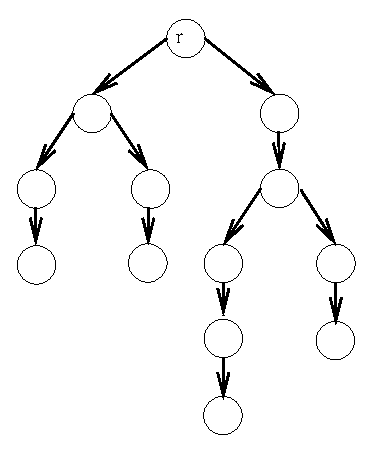
\includegraphics{./figs/arborescencia.eps}
  \caption{\label{fig:arborescencia} Ilustra��o de uma arboresc�ncia 
    que tem com raiz o n� $r$.
  }
 \end{center}
 \end{figure}


Suponha que $(N,E)$ seja uma arboresc�ncia e  
%%%%%%%%%%%%%%%%%%%%%%%%%%%%%%%%%%%%%%%%%%%%%%%%%%%%%%%%%%%%
$f$ uma \defi{fun��o r\'otulo}\index{funcao@fun��o!rotulo@r�tulo} 
que associa a cada n\'o em $N$ um v�rtice em $V(\Qcal)$. 
Se 
\begin{eqnarray*}
 R:=\seq{u_{0}, u_{1}, \ldots, u_{q}}
\end{eqnarray*}
for um caminho em  $(N,E)$, ent�o
\begin{eqnarray*}
 f(R):=\seq{f(u_{0}), f(u_{1}), \ldots, f(u_{q})}
\end{eqnarray*}
ser� uma seq��ncia de v�rtices dos caminhos em $\Qcal$.
Diremos que $(N,E,f)$ � \defi{�rvore dos prefixos} de $\Qcal$ se 
\begin{enumerate}[(p1)]
\item para cada caminho $R$ em $(N,E)$ com in�cio na
      raiz, $f(R)$ for prefixo de algum caminho em $\Qcal$; 
\item para cada prefixo $Q$ de algum caminho em $\Qcal$
      existir um caminho $R$ em $(N,E)$ com in�cio na
      raiz tal que $f(R)=Q$; e
\item o caminho $R$ do item anterior for �nico. 
\end{enumerate}

N�o � verdade que para cada cole��o $\Qcal$ de caminhos em
um grafo existe uma �rvore dos prefixos de $\Qcal$.
Basta existirem em $\Qcal$ caminhos com pontas iniciais distintas
para que n�o seja poss�vel definir a fun��o r�tulo para a raiz da 
arboresc�ncia de forma a satisfazer~(p1).
No entanto, se todos os caminhos em $\Qcal$
tiverem a mesma ponta inicial, ent�o existe uma �rvore dos prefixos de
$\Qcal$ e esta � �nica. Na figura~\ref{fig:prefixo}(b) vemos 
a ilustra��o da �rvore dos prefixos de quatro caminhos de $s$ a~$t$ no grafo
da figura~\ref{fig:prefixo}(a). Na �rvore da ilustra��o, $w,x,y$ 
e $z$ s�o n\'os e $f(w)=s, f(x)=a, f(y)=d$ e $f(z)=d$.

\begin{figure}[htbp]
 \begin{center}
    \psfrag{(a)}{$\iten{a}$}
    \psfrag{(b)}{$\iten{b}$}
    \psfrag{a}{{$s$}}
    \psfrag{b}{{$a$}}
    \psfrag{c}{{$b$}}
    \psfrag{d}{{$c$}}
    \psfrag{e}{{$d$}}   
    \psfrag{f}{{$t$}}
    \psfrag{x}{{$x$}}
    \psfrag{y}{{$y$}}
    \psfrag{z}{{$z$}}
    \psfrag{w}{{$w$}}
    \psfrag{r}{{$r$}}
    \psfrag{grafo}{grafo}
    \psfrag{arvore dos prefixos}{�rvore dos prefixos}
  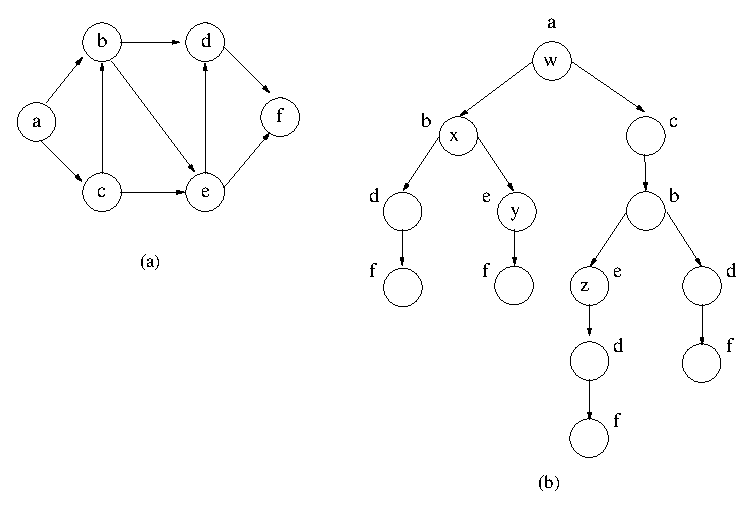
\includegraphics{./figs/prefixo.eps}
  \caption[Exemplo de uma �rvore de prefixos.]{\label{fig:prefixo} (b) mostra a �rvore dos prefixos dos
   caminhos
   $\seq{s,a,c,t}$,
   $\seq{s,a,d,t}$,
   $\seq{s,b,a,c,t}$ e 
   $\seq{s,b,a,d,c,t}$ no grafo em~(a).
   Na �rvore, um s�mbolo ao lado de um n\'o � o r\'otulo desse n\'o.
  O s�mbolo  dentro de um n\'o � o seu nome.
  }
 \end{center}
 \end{figure}

\begin{teorema}{da �rvore dos prefixos}%
\index{teorema!da arvore dos prefixos@da �rvore dos prefixos}
\label{teo:prefixo}
Se $\Qcal$ � uma cole��o de caminhos em um grafo, todos com  
ponta inicial em um v�rtice $s$, ent�o existe uma �rvore dos prefixos de
$\Qcal$. Ademais, a �rvore dos prefixos de $\Qcal$ � �nica 
(a menos de isomorfismo). 
\end{teorema}

\begin{prova}
A demonstra��o � por indu��o no n�mero de caminhos em $\Qcal$.

Se $\Qcal$ tem apenas um caminho, ent�o tomamos 
\begin{align}
N & :=  V(\Qcal), \nonumber \\
E & :=  A(\Qcal), \, \, \mbox{e} \nonumber \\
f(v) & :=  v, \, \, \mbox{para todo $v$ em $N$}. \nonumber
\end{align}

� evidente que $(N,E,f)$ satisfaz (p1), (p2) e (p3) e portanto � 
uma �rvore de prefixos de $\Qcal$.

Suponha agora que $\Qcal$ tem mais do que um caminho e seja
$P$ um caminho qualquer em $\Qcal$. Defina $\Qcal' := \Qcal - \{P\}$.
Por indu��o, existe $(N',E',f')$ �rvore dos prefixos de $\Qcal'$.
Seja $Q_P$ o maior prefixo de $P$ para o qual existe um caminho $R_P$
em $(N',E')$ com in�cio na raiz e tal que $f(R_P)=Q_P$. Temos que $Q_P$ tem 
pelo menos um v�rtice pois todos os caminhos em $\Qcal'$ tem in�cio 
em $s$ e portanto, por (p1), o r�tulo da raiz de $(N',E')$ � $s$.

Suponha 
\begin{align}
P & =\seq{s=v_0,v_1,\ldots,v_k,v_{k+1},\ldots,v_q}, \nonumber \\ 
Q_P & =\seq{s=v_0,v_1,\ldots,v_k}, \,\, \mbox{e} \nonumber \\
R_P & =\seq{u_0,u_1,\ldots,u_k} \, . \nonumber
\end{align}
Como $(N',E',f')$ � arvore de prefixos de $\Qcal'$, ent�o 
$f'(u_i) = v_i$ para $i=0,\ldots,k$.

Para $i=k+1,\ldots,q$, seja $u_i$ um elemento que n�o est� em $N'$ e defina
\begin{align}
N & := N' \cup \{u_{k+1},\ldots,u_{q}\}, \nonumber \\
E & := E' \cup \{u_iu_{i+1} : i = k, \ldots, q-1\}, \, \, \mbox{e}\nonumber \\
f(u) &:= \begin{cases}
          f'(u), & \mbox{se $u\in N'$}, \\
          v_i,   & \mbox{se $u=u_i$ para algum $i$ em $\{k+1,\ldots,q\}$} \, .
        \end{cases} \nonumber
\end{align}
Esta constru��o est� ilustrada na figura~\ref{fig:construcao}.

\begin{figure}[htbp]
 \begin{center}
    \psfrag{(a)}{$\iten{a}$}
    \psfrag{(b)}{$\iten{b}$}
    \psfrag{a}{{$s$}}
    \psfrag{b}{{$a$}}
    \psfrag{c}{{$b$}}
    \psfrag{d}{{$c$}}
    \psfrag{e}{{$d$}}   
    \psfrag{f}{{$t$}}
    \psfrag{x}{{$x$}}
    \psfrag{y}{{$y$}}
    \psfrag{z}{{$z$}}
    \psfrag{w}{{$w$}}
    \psfrag{r}{{$r$}}
    \psfrag{P}{{$P$}}
    \psfrag{Q}{{$Q$}}
    \psfrag{R}{{$R$}}
    \psfrag{grafo}{grafo}
    \psfrag{arvore dos prefixos}{�rvore dos prefixos}
  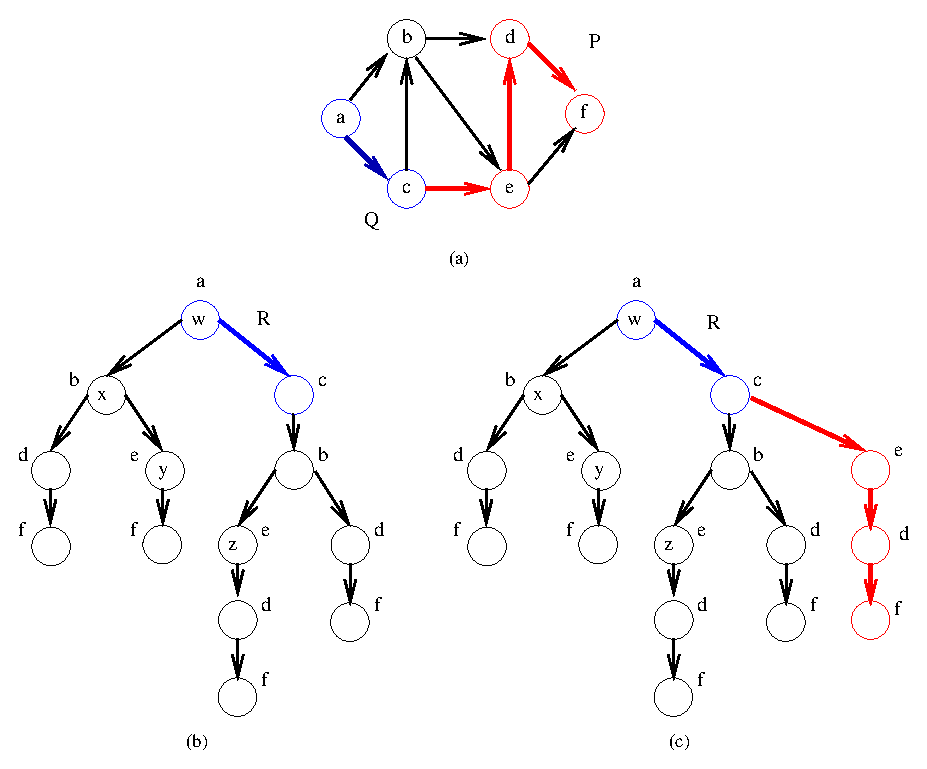
\includegraphics{./figs/construcao.eps}
  \caption[Ilustra��o de uma constru��o de uma �rvore dos prefixos.]{\label{fig:construcao} 
   Ilustra��o da constru��o da �rvore dos
    prefixos de $\Qcal$ a partir da �rvore dos prefixos de 
   $\Qcal'$ feita no teorema~\ref{teo:prefixo}.
   A figura~(a) mostra o caminho $P=\seq{s,b,d,c,t}$ com v�rtices e arcos de 
   cor azul  e vermelha. O prefixo $Q=\seq{s,b}$ tem v�rtices e arco azul.
    Na figura~(b) vemos a �rvore dos prefixos de 
    $\Qcal = \{\seq{s,a,c,t},\seq{s,a,d,t},\seq{s,b,a,c,t},\seq{s,b,d,c,t}\}$.
    Na figura~(c) est�  a �rvore dos prefixos de 
     $\Qcal'= \Qcal -\{P\}$. 
     Nas �rvores dos prefixos os n�s e arcos azuis indicam o caminho $R$
     e  um s�mbolo ao lado de um n\'o � o r\'otulo desse n\'o.}
 \end{center}
 \end{figure}


� claro que
$(N,E)$ � uma arboresc�ncia.  
Passamos a mostrar que $(N,E,f)$ � �rvore de prefixos de $\Qcal$.  

Seja $R$ um caminho em $(N,E)$ com in�cio
na raiz.  Se~$R$ � um caminho em $(N',E')$, ent�o $f(R)=f'(R) $ �
prefixo de algum caminho em $\Qcal'$ que � um subconjunto de $\Qcal$. Se
$R$ utiliza algum n� em $N$ que n�o � n� de $N'$, ent�o $f(R)$ � prefixo
de $P$ que est� em $\Qcal$. Logo, $(N,E,f)$ satisfaz~(p1). 

Para cada prefixo $Q$ de um caminho em $\Qcal'$ existe uma caminho $R$ em 
$(N',E')$ com in�cio na raiz tal que $f'(R)=Q$. 
Como $R$ � um caminho em $(N,E)$ com in�cio na raiz e $f(R)=f(R')$,
conclu�mos que para todo caminho $Q$ em $\Qcal'$ existe um caminho $R$ em
$(N,E)$ tal que $f(R)= Q$. Como o �nico caminho em $\Qcal-\Qcal'$ � $P$ e
$R=\seq{u_0,\ldots,u_q}$ � um caminho em $(N,E)$ com in�cio na raiz 
tal que $f(R)=P$, conclu�mos que  $(N,E,f)$ satisfaz~(p2).
 
Se $Q$ � prefixo de um caminho em $\Qcal'$, ent�o a unicidade do caminho
$R$ em $(N,E)$ com in�cio na raiz tal que $f(R')=Q'$ segue do fato de
$(N',E',f')$ ser �rvore dos prefixos de~$\Qcal'$.  Se $Q$ � um
prefixo de algum caminho em $\Qcal$ que n�o � prefixo de um caminho em
$\Qcal'$ ent�o $Q=\seq{v_0,\ldots,v_k,v_{k+1},\ldots,v_r}$ com 
$k+1 \leq r \leq q$ e portanto, da maximalidade de $Q_P$, segue que  
$R= \seq{u_0,\ldots,u_k,u_{k+1},\ldots,u_r}$ � o �nico caminho em $(N,E)$ 
com origem na raiz e tal que $f(R)=Q$. Com isto acabamos de mostrar
que $(N,E,f)$ tamb�m satisfaz~(p3) e portanto  � �rvore dos prefixos 
de $\Qcal$.

Verifiquemos agora que se $(N_1,E_1,f_1)$ e $(N_2,E_2,f_2)$ s�o �rvores
dos prefixos de uma cole��o de caminhos $\Qcal$ com in�cio em um v�rtice
$s$, ent�o essas �rvores s�o essencialmente a mesma, isto �, s�o
isomorfas.

Definimos uma fun��o $h$ de $N_1$ em $N_2$ que � um isomorfismo entre
$(N_1,E_1,f_1)$ e $(N_2,E_2,f_2)$.  A cada n� $u_1$ em $N_1$
associaremos um n� $h(u_1)$ em $N_2$ da seguinte maneira.  Como
$(N_1,E_1)$ � uma arboresc�ncia temos que existe um �nico caminho
$R_{u_1}$ que tem como in�cio a raiz da arboresc�ncia e como t�rmino
$u_1$.  Devido a~(p1) sabemos que $Q:=f_1(R_{u_1})$ � prefixo de um
caminho em $\Qcal$.  J�, de (p2) e (p3) temos que $R_{u_1}$ � o �nico
caminho com in�cio na raiz tal que $f_1(R_{u_1})=Q$. Novamente, devido
a~(p2) e~(p3), temos que existe na arboresc�ncia $(N_2,E_2)$ um �nico
caminho $R_{u_2}$ com in�cio na raiz tal que $f_2(R_{u_2})=Q$. Seja
$u_{u_2}$ a ponta final de $R_{u_2}$.  Definimos $h(u_{u_1}):=u_2$.

Da unicidade dos caminhos $R_{u_1}$ e $R_{u_2}$ acima segue que $h$ �
uma bije��o entre $N_1$ e $N_2$ e que se $u_1w_1$ � um arco em $E_1$
ent�o $h(u_1)h(w_1)$ � um arco em $E_2$. Al�m disso, para todo $u_1$ em
$N_1$ � evidente que $f_1(u_1) = f_2(h(u_1))$, pois ambos s�o os
t�rminos de um �nico prefixo $Q$ de um caminho em $\Qcal$. Segue do que
foi exposto que $h$ � um isomorfismo entre $(N_1,E_1,f_1)$ e
$(N_2,E_2,f_2)$.


%% Como $(N_1,E_1,f_1)$ e $(N_2,E_2,f_2)$ s�o �rvores dos prefixos de
%% $\Qcal$ temos que para todo prefixo $Q$ de um caminho em $\Qcal$ existe
%% um �nico caminho $R_{Q,1}$ em $(N_1,E_1)$ com origem na raiz e um �nico
%% caminho $R_{Q,2}$ em $(N_2,E_2)$ com origem na raiz tais que
%% $f_1(R_1)=Q$ e $f_2(R_2)=Q$. Seja $u_{Q,1}$ o n� que � a ponta final de
%% $R_1$ e $u_{Q,2}$ o n� que � ponta final de $R_{Q,2}$. Para cada n� $u

\end{prova}






\section{M�todos gen�ricos}
\label{sec:metodo-generico}

A descri��o que fazemos aqui de um m�todo para o \kCM{} �, 
de certa forma, \textit{top-down}. 
Come�aremos com um m�todo gen�rico que ser� refinado a cada passo
incluindo, convenientemente, algumas subrotinas auxiliares.
%%%%%%%%%%%%%%%%%%%%%%%%%%%%%%%%%%%%%%%%%%%%%%%%%%%%%%%%%%%%%%%%%%%%% 
A nossa inten��o aqui � apresentar uma descri��o mais conceitual em que a
corre��o e o consumo de tempo do m�todo sejam um tanto
quanto evidentes, apesar do consumo de tempo ser exponencial.
%%%%%%%%%%%%%%%%%%%%%%%%%%%%%%%%%%%%%%%%%%%%%%%%%%%%%%%%%%%%%%%%%%%%%
Dei\-xa\-re\-mos para a pr�xima se��o a descri��o de um algoritmo que � mais
um refinamento dos m�todos desta se��o e atinge o menor consumo de
tempo conhecido, o algoritmo de Yen.
%%%%%%%%%%%%%%%%%%%%%%%%%%%%%%%%%%%%%%%%%%%%%%%%%%%%%%%%%%%%%%%%%%%%
Assim, esta se��o pretende ser uma ponte entre id�ias gen�ricas e muito
simples e o algoritmo da pr�xima se��o.

O m�todo abaixo recebe um grafo $(V,A)$, uma fun��o custo, dois v�rtices $s$ e
$t$ e um inteiro positivo $k$ e devolve uma lista $\seq{P_1,\ldots,P_k}$ de
$k$-menores caminhos de $s$ a~$t$.

\begin{algoritmo}

\textbf{M�todo} \Generico{} $(V,A,c,s,t,k)$ %\\[2mm]
\index{metodo@m�todo!Generico@\Generico}\index{Generico@\Generico}
   
0\x $\Pcal \larr$ conjunto dos caminhos de $s$ a~$t$ 

1\x \para{} $i=1,\ldots,k$ \faca %\\[1mm]

2\xx  $P_i \larr \mbox{caminho de custo m�nimo em $\Pcal$}$ %\\[1mm]

3\xx  $\Pcal \larr \Pcal - \{P_i\}$

4\x \devolva{} $\seq{P_1,\ldots,P_k}$

\end{algoritmo}

No in�cio de cada itera��o da linha~1 o conjunto $\Pcal$ cont�m os
candidatos a $i$-�simo caminho m�nimo de $s$ a~$t$.  O algoritmo de
Yen � uma elabora��o do m�todo \Generico.  Em vez do conjunto~$\Pcal$,
\YenGenerico{}, descrito logo adiante, mant�m uma parti��o $\Pi$
de~$\Pcal$.  Na linha~6 do m�todo a parti��o $\Pi$ � atualizada.  Em
cada itera��o $i$, � escolhido o caminho mais barato $P_i$ dentre os
caminhos em um conjunto $\Lcal$ formado por \textit{um} caminho m�nimo
$P_{\pi}$ representante de cada parte $\pi$ de~$\Pi$. Na linha~6 do
m�todo a parti��o $\Pi$ � atualizada.  O m�todo mant�m ainda um
conjunto $\Qcal$ com cada caminho em $\seq{P_1,\ldots,P_i}$.

%\newpage

\begin{algoritmo}

\textbf{M�todo} \YenGenerico{} $(V,A,c,s,t,k)$ %\\[2mm]
\index{metodo@m�todo!YenGenerico@\YenGenerico}%
\index{YenGenerico@\YenGenerico}
   
0\x $\Pi \larr \{\mbox{conjunto dos caminhos de $s$ a~$t$}\}$

1\x $\Qcal \larr \emptyset $

2\x \para{} $i=1,\ldots,k$ \faca %\\[1mm]

3\xx  $\Lcal  \larr \{P_{\pi} : P_{\pi} \ \mbox{� caminho m�nimo na parte $\pi$
de~$\Pi$}\}$

4\xx  $P_i \larr \mbox{caminho de custo m�nimo em $\Lcal$}$ %\\[1mm]

5\xx  $\Qcal \larr \Qcal \cup \{P_i\}$

6\xx  $\Pi \larr \AtualizeGenerico~(V,A,s,t,\Qcal)$

7\x \devolva{} $\seq{P_1,\ldots,P_k}$

\end{algoritmo}

Na pr�xima se��o tratamos de
$\Pi$ de uma maneira mais precisa e s� depois, ao final da se��o,
consideramos os detalhes da subrotina \AtualizeGenerico.
Como veremos, a efici�ncia do algoritmo de Yen, descrito na
se��o~\ref{sec:algoritmo-de-yen}, depende fortemente da estrutura
restrita dos caminhos nas partes de~$\Pi$: cada parte � formada por
caminhos que t�m um certo prefixo comum.


Neste ponto, como no in�cio de cada execu��o do bloco de linhas
2--6  do m�todo \YenGenerico{} temos que 
\begin{quote}
$\Pi$ � uma parti��o de $\Pcal=\Pcal_{st}-\Qcal$,
\end{quote}
ent�o a corre��o do m�todo � evidente.

\begin{teorema}{da corre��o de \YenGenerico}%
\index{teorema!da correcao de YenGenerico@da corre��o de \YenGenerico}%
\index{YenGenerico@\YenGenerico!correcao@corre��o} 
Dado um grafo $(V,A)$, uma fun��o
custo~$c$ e  v�rtices $s$ e $t$ o m�todo \YenGenerico\ corretamente
encontra os $k$-menores caminhos de $s$ a~$t$.
\fimprova{}
\end{teorema}





%%%%%%%%%%%%%%%%%%%%%%%%%%%%%%%%%%%%%%%%%%%%%%%%%%%%%%%%%%%%%%%%%%%%%%%%
%%%%%%%%%%%%%%%%%%%%%%%%%%%%%%%%%%%%%%%%%%%%%%%%%%%%%%%%%%%%%%%%%%%%%%%%
\section{Parti��o de caminhos}
\label{sec:particao}

Seja $\Pcal_{st}$ a cole��o
dos caminhos de $s$ a~$t$ em $(V,A)$.
%%%%%%%%%%%%%%%%%%%%%%%%%%%%%%%%%%%%%%%
Suponha que $\Qcal$ seja uma cole��o  de 
caminhos distintos de $s$ a~$t$, como, por exemplo, 
a atualizada na linha~5 do m�todo \YenGenerico{}.  
Passamos a des\-cre\-ver a parti��o
$\Pi$ dos caminhos em $\Pcal := \Pcal_{st} - \Qcal$.
Para isto � conveniente utilizarmos a 
\textit{�rvore dos prefixos} de $\Qcal$, como foi feito por John Hershberger,
Matthew Maxel e Subhash Suri~\cite{hershberger:acmta-3-??}.

No que segue suponha que $(N,E,f)$ � 
a �rvore dos prefixos de $\Qcal$ e $u$ � um n\'o qualquer em $N$.
%%%%%%%%%%%%%%%%%%%%%%%%%%%%%%%%%%%%%%%%%%%%%%%%%%%%%%%%%
Representaremos por $R_u$\mar{$R_u$} o
caminho da raiz a $u$ na �rvore. 
Assim,  $f(R_u)$\mar{$f(R_u)$} �
o prefixo de um caminho em $\Qcal$. 
Por exemplo, na �rvore dos prefixos da figura~\ref{fig:prefixo}(b)
temos que $R_y = \seq{w,x,y}$ e $f(R_y) = \seq{s,a,d}$.

Seja\mar{$A_u$}
%$A_u$ a
%cole��o dos arcos em $A$ com ponta inicial em $f(u)$ e
%ponta final $f(w)$ para todo arco $uw$ em $E$, isto �,
\begin{eqnarray*}
A_u := \{ f(u)f(w) : uw \in E\}. 
\end{eqnarray*}  
e seja $\pi_u$\mar{$\pi_u$} o conjunto dos caminhos em $\Pcal$ com
prefixo $f(R_u)$ e que n�o possuem arcos em~$A_u$.
Para o exemplo na figura~\ref{fig:prefixo} temos que: 
\begin{eqnarray*}
A_w = \{sa,sb\}, 
A_x = \{ac,ad\}, 
A_y = \{dt\} \ \mbox{e} \ 
A_z = \{dc\} \\
%\pi_r = \emptyset,
\pi_w = \emptyset,
%\pi_w = \{\seq{s,b,a,d,c,t}  \}, 
\pi_x = \emptyset,
\pi_y = \{\seq{s,a,d,c,t}\},  \ \mbox{e} \
\pi_z = \{\seq{s,b,a,d,t}\}.  
\end{eqnarray*}

Notemos que para cada n� $u$ que � folha de $(N,E,f)$ temos que
$\pi_u$ � formado pelo caminho $f(R_u)$ de $\Qcal$. Portanto, o n�mero
de folhas de $(N,E,f)$ � exatamente $|\Qcal|$.

A parti��o~$\Pi$\mar{$\Pi$}\index{$\Pi$} � formada por uma parte $\pi_u$ para
cada v�rtice $u$ em $N$ que \textit{n�o} � folha, ou seja,
\[
\Pi := \{\pi_u : u \in N, u \, \mbox{n�o � folha}\}.
\]
Notemos que para cada cole��o $\Qcal$ de caminhos temos 
uma �nica �rvore dos prefixos $(N,E,f)$ de $\Qcal$ e 
associada a essa �rvore temos uma �nica parti��o $\Pi$ de $\Pcal$. 
Assim, algumas vezes nos referiremos a $\Pi$ como sendo a 
\defi{parti��o associada}\index{particao associada@parti��o associada} 
� cole��o $\Qcal$.

Podemos verificar que cada caminho em $\Qcal$ n�o pertence a
nenhuma parte de~$\Pi$. 

\begin{teorema}{da parti��o}%
\index{teorema!da particao@da parti��o}
\label{teo:particao}
%Considere uma execu��o do algoritmo \AtualizeGenerico{} $(V,A,s,t,\Qcal)$.
Sejam $(V,A)$ um grafo, 
$s$ e $t$ dois de seus v�rtices e~$\Qcal$ uma cole��o de caminhos 
de~$s$ a~$t$ em~$(V,A)$. 
Se $P$  � um caminho de~$s$ a~$t$ que n�o est� em~$\Qcal$, ent�o~$P$ pertence
a uma �nica parte de~$\Pi$. 
\end{teorema}
\begin{prova}
Considere um caminho $P$ que n�o est� em $\Qcal$.  Suponha que
$Q$ � o maior prefixo de  $P$ que tamb�m � prefixo de algum caminho em $\Qcal$. 
Como $P$ n�o est� em $\Qcal$ ent�o $Q$ � um prefixo pr�prio de $P$. 
Como $(N,E,f)$ � �rvore dos prefixos de $\Qcal$, 
ent�o, por (p2) e (p3), existe um �nico caminho $R$ com in�cio na raiz e 
t�rmino em um n� interno da �rvore 
tal que $f(R)=Q$ � prefixo de $P$. Se $u$ � o n� interno da �rvore que 
� a ponta final de $R$, ent�o,
pela maximalidade de $Q$, temos que $P$ n�o possui arcos em $A_u$.
Portanto, $P$ est� na parte $\pi_u$ e portanto esta
� a �nica parte de 
$\Pi$ que cont�m $P$. 
\end{prova}


Notemos que, cada parte
$\pi_u$ em que $u$ � folha, � formada pelo �nico caminho $P$ em $\Qcal$
tal que $f(R_u)=P$. Assim, do teorema~\ref{teo:particao} da parti��o
segue o color�rio abaixo.

\begin{corolario}{}
Seja $\Qcal$ uma cole��o de caminhos em um grafo $(V,A)$
tal que todos os caminhos em $\Qcal$ t�m ponta inicial em 
um v�rtice $s$ e ponta final em um v�rtice $t$.
Se $(N,E,f)$ � a �rvore dos prefixos de $\Qcal$, ent�o 
\[
\Pcal_{st} = \bigcup_{u \in N} \pi_u \,,
\]
onde $\Pcal_{st}$ � a cole��o de todos os caminhos de $s$ a $t$ 
em $(V,A)$.  \fimprova
\end{corolario}


Agora temos em m�os todos os elementos necess�rios para voltarmos a
discutir o  m�todo~\YenGenerico{} e complet�-lo. 
No in�cio de cada itera��o da
linha~2 do m�todo \YenGenerico{}, o n�mero de partes em $\Pi$ � igual ao n�mero de n�s, que n�o s�o folhas, na �rvore dos prefixos de $\Qcal$ e, portanto, � certamente n�o
superior a $i \times n$. Logo, no in�cio de cada itera��o, o n�mero
de caminhos em $\Lcal$ � n�o superior a $i \times n$, j� que a �rvore
dos prefixos de $\Qcal$ n�o possui mais do que $n$ n�s para cada
caminho em $\Qcal$.


O algoritmo \AtualizeGenerico{} resume toda a discuss�o acima.  Este
algorimo recebe um grafo $(V,A)$, dois v�rtices $s$ e $t$ do grafo e uma
cole��o $\Qcal$ de caminhos de $s$ a $t$ e devolve uma parti��o $\Pi$
dos caminhos em $\Pcal = \Pcal_{st}-\Qcal$.

\begin{algoritmo}

\textbf{Algoritmo} \AtualizeGenerico{} $(V,A,s,t,\Qcal)$ %\\[2mm]
\index{algoritmo!AtualizeGenerico@\AtualizeGenerico}%
\index{AtualizeGenerico@\AtualizeGenerico}
   
0\x $\Pi \larr \emptyset \quad \quad \Pcal \larr \Pcal_{st} - \Qcal$

1\x $(N,E,f) \larr$ �rvore dos prefixos de $\Qcal$

2\x \para{} \cada{} $u \in N$ que n�o � uma folha \faca %\\[1mm]

3\xx  $\pi_u \larr \{\mbox{caminhos em $\Pcal$ com prefixo $f(R_u)$}$

\xxxxx \quad e que n�o possuem arcos em $A_u \}$

4\xx  $\Pi \larr  \Pi \cup \{\pi_u\}$ %\\[1mm]

5\x \devolva{} $\Pi$

\end{algoritmo}


%% Tamb�m podemos verificar que cada
%% caminho $P$ em $\Pcal$ est� em uma �nica 
%% parte de~$\Pi$. De fato, seja $P'$ o maior prefixo de~$P$ 
%% que � prefixo de algum caminho em $\Qcal$. Pela defini��o
%% de �rvore de prefixos, existe um �nico caminho $R'$ em 
%% $(N,E)$ com in�cio na raiz e tal que $P' = f(R')$. 
%% Para o v�rtice $u$ t�rmino de $R'$ temos que $P$ est� em
%% $\pi_u$ e � a �nica parte que possui $P$. 


%% ???Ainda utilizando a estrutura da �rvore dos prefixos de  

As �rvores dos prefixos de duas execu��es consecutivas do algoritmo
\AtualizeGenerico{} s�o muito semelhantes: apenas um novo caminho �
acrescentado � �rvore anterior.  Isto, em particular, significa que as
parti�\~oes de duas itera�\~oes consecutivas das linhas 2--6 do m�todo
\YenGenerico{} s�o muitos semelhantes. Esta observa��o pode ser
utilizada para que um refinamento do algoritmo \AtualizeGenerico{}
obtenha, mais eficientemente, uma nova parti��o a partir da anterior. 
Veremos este e outro refinamento na pr�xima se��o.
 





\section{Algoritmo de Yen}
\label{sec:algoritmo-de-yen}

O algoritmo que Jin Y. Yen~\cite{yen:ms-17-712} desenvolveu para resolver
o \kCM{} parece ter um papel central dentre os algoritmos que foram
posteriormente projetados para o \kCM\ ou mesmo para vers\~oes mais
restritas do
problema~\cite{eppstein:siamjc-28-652,katoh:n-12-411,hershberger:acmta-3-??}.
V�rias melhorias pr�ticas do m�todo de Yen foram implementadas e
testadas~\cite{brander:370,eleni:n-34-88,martins:qjbfiors-1-121,martins:relatorio,perko:n-16-149}.

Antes de prosseguirmos, mencionamos que o algoritmo de Yen foi generalizado por
Eugene L. Lawler~\cite{lawler:ms-18-401} para problemas de otimiza��o
combinat\'oria, contanto que seja fornecida uma subrotina para determinar uma
solu��o \'otima sujeita � condi��o de que certas vari�veis tenham seus valores
fixados. Por exemplo, no caso do algoritmo de Yen para o \kCM{} essa subrotina
resolve o seguinte \defi{problema do subcaminho m�nimo}\index{problema!do
subcaminho m�nimo@do subcaminhos m�nimo}, denotado por \PSM:
 \begin{quote}
   \textbf{Problema} \PSM$(V,A,c,s,t,Q,F)$:%
   \index{problema!PSM@\PSM}\mar{\PSM}
   %%%%%%%%%%%%%%%%%%%%%%%%%%%%%%%%%%%%%%%%%%%%%%%%%%%%%%%%%%%%%%%%%%%
   Dado um grafo $(V,A)$, uma fun��o
   custo $c$, dois v�rtice $s$ e $t$, um caminho $Q$ e uma parte $F$ de $A$, 
   encontrar um caminho de custo m�nimo 
   de $s$ a~$t$ que tem $Q$ como prefixo e n�o cont�m arcos em $F$.
 \end{quote}
� evidente que se $Q$ n�o tem in�cio em $s$ ent�o o problema �
invi�vel. Do ponto de vista do m�todo de Lawler, o prefixo $Q$ e o 
conjunto $F$ s�o as `vari�veis' com valores fixados. 
 
Resolver o \PCM$(V,A,c,s,t)$ � o mesmo que resolver o
\PSM$(V,A,c,s,t,\seq{s},\emptyset)$.  Por outro lado, o
\PSM{} pode ser solucionado aplicando-se um algoritmo para o
\PCM{} em um subgrafo $(V',A')$ apropriado de $(V,A)$:
\begin{align}
V' & := V - (V(Q)-\{s'\}) \nonumber \\
A' & := A - F - A^+(Q-{s'}) - A^-(Q) \, , \nonumber 
\end{align}
onde 
$V(Q)$ � o conjunto dos v�rtices em $Q$, 
$A^+(Q)$ s�o os arcos com ponta inicial em $V(Q)$, 
$A^-(Q)$ s�o os arcos com ponta final em $V(Q)$ e
$s'$ � a ponta final de $Q$.
Desta forma, o
\PCM{} e o \PSM{} s�o computacionalmente equivalentes e ambos
podem ser resolvidos consumindo-se tempo~$T(n,m)$.


%%%%%%%%%%%%%%%%%%%%%%%%%%%%%%%%%%%%%%%%%%%%%%%%%%%%%%%%%%%%%%%%
Voltemos ao algoritmo de~Yen.
Conceitualmente, o algoritmo de Yen � uma elabora��o do algoritmo 
\YenGenerico. Como no m�todo \YenGenerico, no in�cio de cada itera��o
$\Lcal$ � uma lista dos candidatos a $i$-�simo caminho m�nimo de $s$
a~$t$. Esta lista � formada por um caminho m�nimo em cada parte da
parti��o $\Pi$. O algoritmo de Yen  mant�m o conjunto $\Qcal$ dos 
caminhos previamente selecionados atrav�s de sua
�rvore dos prefixos $(N,E,f)$. Diferentemente 
do m�todo \YenGenerico{}, o algoritmo de Yen
armazena a parti��o $\Pi$ implicitamente atrav�s
da �rvore dos prefixos $(N,E,f)$ e de $\Lcal$: 
\begin{eqnarray}
\label{eq:caminhos}
\parbox[c]{12cm}{para cada n� $u$ em $(N,E,f)$ que n�o � folha a lista 
$\Lcal$ cont�m um caminho de custo m�nimo na parte $\pi_u$ de $\Pi$.}
\end{eqnarray}
Pelo teorema~\ref{teo:particao} da parti��o temos que $\Lcal$ cont�m um 
caminho de custo m�nimo de cada parte da parti��o $\Pi$ de $\Pcal_{st}-\Qcal$.
A tarefa de cada itera��o � escolher  o caminho $P$ mais barato dentre 
todos em $\Lcal$  e, em seguida, atualizar $\Lcal$ e
%%%%%%%%%%%%%%%%%%%%%%%%%%%%%%%%%%%%%%%%%%%%%%%%%%%%%%%%%%%%%%%%%%%%%%%
%a parti��o s�o \textit{levemente} atualizada atrav�s da atualiza��o da
%%%%%%%%%%%%%%%%%%%%%%%%%%%%%%%%%%%%%%%%%%%%%%%%%%%%%%%%%%%%%%%%%%%%%%
a �rvore dos prefixos $(N,E,f)$ dos caminhos selecionados. 
Essa atualiza��o � feito na linha~5 pelo algoritmo~\Atualize. 

O algoritmo \Atualize{} recebe um grafo $(N,A)$, uma fun��o custo $c$,
v�rtices $s$ e $t$, um caminho $P$ de $s$ a $t$, 
a �rvore dos prefixos $(N',E',f')$ de
uma cole��o $\Qcal'$ de $st$-caminhos e uma lista $\Lcal'$ de
$st$-caminhos tais que:
\begin{quote}
$(N',E',f')$ e $\Lcal'$ satisfazem \eqref{eq:caminhos} nos
  pap�is de $(N,E,f)$ e $\Lcal$
\end{quote}
e devolve: 
\begin{quote}
uma �rvore dos prefixos $(N,E,f)$ da cole��o $\Qcal = \Qcal' \cup
\{P\}$ de $st$-caminhos e uma lista $\Lcal$ de $st$-caminhos que
satisfazem \eqref{eq:caminhos}.
\end{quote}


%% Ao inv�s da parti��o  $\Pi$ 
%% de $\Pcal$, Yen mant�m em $\Lcal$ um caminho m�nimo de
%% cada parte de $\Pi$. 
%%%%%%%%%%%%%%%%%%%%%%%%%%%%%%%%%%%%%%%%%%%%%%%%%%%%%%%%%%%%%%%%%
%de $\Pcal$ em n�o mais do que $2i$ partes e uma lista $L$ com 
%um caminho mais barato de cada uma das partes. 

\begin{algoritmo}

\textbf{Algoritmo} \Yen{} $(V,A,c,s,t,k)$ %\\[2mm]%
\index{algoritmo!Yen@\Yen}\index{Yen@\Yen}
   
0\x $P \larr $ um caminho de custo m�nimo de $s$ a $t$

1\x $\Lcal \larr \{P\}$

2\x $(N,E,f) \larr $ �rvore dos prefixos de $\Lcal$ %\quad {$\rhd$  �rvore vazia} 

3\x \para{} $i=1,\ldots,k$ \faca %\\[1mm]

4\xx  $P_i \larr \mbox{caminho de custo m�nimo em $\Lcal$}$
%\\[1mm]

%5\xx  $\Lcal \larr \Lcal \setminus \{P_i\}$

%5\xx  $\Qcal \larr \Qcal \cup \{P_i\}$

5\xx  $(N,E,f,\Lcal) \larr \Atualize~(V,A,c,s,t,P_i,N,E,f,\Lcal)$

6\x \devolva{} $\seq{P_1,\ldots,P_k}$

\end{algoritmo}

Tendo em vista a especifica��o do algoritmo~\Atualize{} a corre��o do
algo\-rit\-mo~\Yen{} � evidente. 


\begin{teorema}{da corre��o de \Yen}%
\index{teorema!da correcao de Yen@da corre��o de \Yen}%
\index{Yen@\Yen!correcao@corre��o}
 Dado um grafo $(V,A)$, uma fun��o
 custo~$c$ e  v�rtices $s$ e $t$ o algoritmo \Yen\ corretamente
   encontra os $k$-menores caminhos de $s$ a~$t$.
\fimprova{}
\end{teorema}



O algoritmo~\Atualize{} que est� logo a seguir utiliza como subrotina o
algoritmo
\ArvorePrefixos\index{algoritmo!ArvorePrefixos@\ArvorePrefixos}\index{ArvorePrefixos@\ArvorePrefixos}
que recebe uma �rvore dos prefixos de uma cole��o de caminhos $\Qcal'$
com ponta inicial em um v�rtice $s$ e um caminho $P$ com ponta inicial
em $s$  e devolve a �rvore dos prefixos de
$\Qcal = \Qcal' \cup \{P\}$. O servi�o feito por \ArvorePrefixos{} �
essencialmente descrito na demonstra��o do teorema~\ref{teo:prefixo}
e est� ilustrado na figura~\ref{fig:prefixo}.



%%Na verdade, com o n�mero dos caminhos em $\Pcal$ � muito grande


\begin{algoritmo}

\textbf{Algoritmo} \Atualize{} $(V,A,c,s,t,P,N',E',f',\Lcal')$ %\\[2mm]
\index{algoritmo!Atualize@\Atualize}\index{Atualize@\Atualize}
   
   
0\x $\Lcal \larr \Lcal' - \{P\}$

1\x $R_P \larr $ maior caminho em $(N',E')$ com ponta inicial na raiz tal que

\xxxxx $Q_P := f(R_P)$ � prefixo de $P$


2\x $(N,E,f) \larr$ \ArvorePrefixos $(N',E',f',P)$


3\x Suponha que $\seq{u_0,\ldots,u_k,u_{k+1},\ldots,u_q}$ � o caminho em 
$(N,E)$ tal que

\xxxx $R_P = \seq{u_0,\ldots,u_k}$ e $f(\seq{u_0,\ldots,u_k,u_{k+1},\ldots,u_q}) = P$.


4\x \para{} \cada{} $u \in \{u_k,\ldots,u_{q-1}\}$ \faca %\\[1mm]

5\xx  $P_u \larr \mbox{caminho de $s$ a~$t$ de custo m�nimo com prefixo $f(R_u)$}$

\xxxxx e que n�o possui arcos em $A_u$

6\xx  $\Lcal \larr  \Lcal \cup \{P_u\}$ %\\[1mm]

7\x \devolva{} $(N,E,f,\Lcal)$


\end{algoritmo}

Primeiramente, como o algoritmo \Atualize{} recebe
a �rvore dos prefixos $(N',E',f')$ 
de uma cole��o de caminhos $\Qcal'$ com origem em 
um v�rtice $s$ e um caminho $P$ com origem em $s$ ent�o, devido � especifica��o do algoritmo \ArvorePrefixos{}
invocado na linha~2, � claro que 
\Atualize{} corretamente devolve a �rvore dos prefixos $(N,E,f)$ de
$\Qcal = \Qcal' \cup \{P\}$.

Pela linha~1 do algoritmo \Atualize{} temos que $Q_P$ � o maior prefixo de $P$ 
para o qual existe um caminho $R_P$ na �rvore dos prefixos $(N',E',f')$ 
de $\Qcal'$ tal que $f'(R_p)=Q_P$.
Devido � defini��o  do caminho $\seq{u_0,\ldots,u_k,u_{k+1},\ldots,u_q}$ 
feita na linha~3 e � defini��o de $R_P$ temos que o caminho 
$P$ � o representante da parte $\pi'_{u_k}$ da parti��o $\Pi'$ associada � �rvore dos prefixos $(N',E',f')$.
Seja $\Pi$ a parti��o associada � �rvore dos prefixos $(N,E,f)$ constru�da na 
linha~2.
Antes da primeira execu��o do bloco de linhas 4--6 temos que 
$\Lcal$ cont�m um caminho de custo m�nimo de cada parte $\pi'_u=\pi_u$, 
onde $u$ � um n� em $N-\{u_k,\ldots,u_{q-1}\}$. 
Nas linhas 4-5, s�o acrescidos a $\Lcal'$ os caminhos de custo m�nimo 
em $\pi_{u}$ para $u$ em $\{u_k,u_{k+1}, \ldots, u_{q-1}\}$, que s�o os
n�s em $N-N'$ que n�o s�o folhas, j� que a �nica folha de $(N,E,f)$ 
em $N-N'$ � $u_q$.
Assim, conclu�mos que $\Lcal$ devolvida cont�m, para cada n� $u$ da �rvore dos prefixos $(N,E,f)$ de $\Qcal$ que n�o � folha,
um caminho de custo m�nimo na parte $\pi_u$.
Com isto conclu�mos que o algoritmo~\Atualize{} faz o que promete.


%% \begin{teorema}{da corre��o de \Atualize}
%%  Dado um grafo $(V,A)$, uma fun��o
%%  custo~$c$, v�rtices $s$ e $t$, uma lista $\Lcal{}$
%% de caminhos de $s$ o algoritmo \Yen\ corretamente
%% encontra os $k$-menores caminhos de $s$ a~$t$.
%% \end{teorema}

%% \begin{prova}

%% \end{prova}


Em cada execu��o do bloco de linhas 3--5 do algoritmo \Yen{} 
o n�mero de caminhos em $\Lcal$ � n�o superior a $k \, n$.
Assim, o consumo de tempo de todas as execu��es da linha~4 � 
$\Oh(k \lg kn)$, se utilizamos um min-heap para armazenarmos 
os custos dos caminhos em $\Lcal$.
O  consumo de tempo do algoritmo \Yen{} � dominado pelo consumo 
de tempo de todas as execu��o da linha~5, ou seja,  
pelo consumo de tempo de das $k$ execu��es do algoritmo \Atualize.

A cada execu��o da linha~5 do algoritmo \Atualize{}, na verdade, 
estamos resolvendo o problema \PSM $(V,A,c,s,t,f(R_u),A_u)$. 
Assim, o consumo de tempo de cada execu��o dessa linha � $T(n,m)$.
Essa linha~5 � executada uma vez para cada n� na �rvore dos prefixos 
dos $k$-menores caminhos $\seq{P_1,\ldots,P_k}$. Como o n�mero de n�s nessa
�rvore � n�o superior a $k\, n$, conclu�mos que o consumo de 
tempo total das execu��es dessa linha �  $\Oh(k\, n\, T(n,m))$.


%% O 
%%   algoritmo resultante � $n \, i \, T(n,m))$. Em chamadas consecutivas do
%%   algoritmo \Atualize{}, as �rvores dos prefixos calculadas s�o muito
%%   semelhantes.
%% %Logo, � poss�vel fazermos com que o consumo de tempo seja $n \, T(n,m)$.
%% De fato, o algoritmo  pode ser implementado de tal maneira
%% que o consumo o seu consumo de tempo seja $n \, T(n,m)$.

%% O algoritmo de \Yen{} pode ser implementado de tal maneira que o seu consumo de
%% tempo seja proporcional a $k \, n \, T(n,m)$.

\begin{teorema}{do consumo de tempo de \Yen}%
\index{teorema!do consumo de tempo de Yen@do consumo de tempo de \Yen}%
\index{Yen@\Yen!consumo de tempo}
O consumo de tempo do algoritmo~\Yen{} �  $\Oh(k\, n\, T(n,m))$, onde
$n$ � o n�mero de v�rtices e $m$ � o n�mero de arcos do 
grafo dado, respectivamente.
\fimprova{}
\end{teorema}



\section{Revis�o algor�tmica}
 
Antes de Yen, o problema \kCM{} � uma generaliza��o do
problema dos caminhos m�nimos que havia sido considerado por v�rios
autores. 
Aqui fazemos uma breve revis�o dos trabalhos produzidos por esses autores.


Todos os algoritmos para o \kCM{} podem ser aplicados a grafos com
custos negativos mas sem circuito negativo. No caso de grafos com
custos negativos, os algoritmos devem utilizar o algoritmo de Richard
Ernest Bellman~\cite{bellman} e Lester Randolph Ford~\cite{ford} em
vez do algoritmo de Dijkstra. O consumo de tempo do algoritmo de
Bellman-Ford � $\Oh(mn)$.

%%%%%%%%%%%%%%%%%%%%%%%
%% Bock, Kantner and Haynes
Bock, Kantner e Haynes~\cite{bock}, em 1957, desenvolveram um algoritmo
semelhante ao m�todo \Generico{} que enumerava todos os caminhos entre
$s$ e $t$, ordenava-os de acordo com seus custos e depois devolvia os
$k$-menores caminhos.  Essa estrat�gia utiliza tempo e mem�ria
exponencial e s� pode fazer sentido em utiliz�-la se $k$ for
extremamente grande.

%%%%%%%%%%%%%%%%%%%%%%%
%%
Em 1961, Pollack~\cite{pollack} prop�s um algoritmo que para obter os
$k$-menores caminhos primeiro constru�a os $(k-1)$-menores caminhos e
depois, para todo conjunto de $k-1$ arcos, um de cada caminho,
encontrava um caminho m�nimo de $s$ a $t$ que n�o passava por esses
arcos. Depois disto, o algoritmo, escolhia determinava o $k$-�simo menor
caminho dentre todos os caminho encontrados. 
O algoritmo de Pollack pode ser aplic�vel quando $k$ � pequeno, mas o seu consumo de tempo cresce exponencialmente com o valor de $k$.


%%%%%%%%%%%%%%%%%%%%%%%%%%%%%%%%%%%%%%%%%%%%%%%%%%%%%%%%%%%%%%%
%\newpage
\begin{algoritmo}

\textbf{Algoritmo} \Pollack{} $(V,A,c,s,t,k)$ %\\[2mm]
\index{algoritmo@Pollacko@\Pollack}\index{Pollack@\Pollack}
   
%0\x $\Pcal \larr \mbox{conjunto dos caminhos de $s$ a~$t$}$ 

0\x $P_1 \larr$ um $st$-caminho de custo m�nimo em $(V,A)$

1\x \para{} $i=2,\ldots,k$ \faca %\\[1mm]

2\xx  $\Lcal \larr \emptyset$

3\xx  $\Acal \larr \{\{a_1,\ldots,a_{i-1}\}: a_k \, \mbox{� arco em $P_k$}\}$

4\xx  \para{} \cada{} $U$ em $\Acal$ \faca

5\xxx    $P_U \larr$ $st$-caminho de custo m�nimo em $(V,A-U)$

6\xxx    $\Lcal \larr \Lcal \cup \{P_U\}$
 

7\xx  $P_i \larr \mbox{caminho de custo m�nimo em $\Lcal$}$ %\\[1mm]

8\x \devolva{} $\seq{P_1,\ldots,P_k}$

\end{algoritmo}


%%%%%%%%%%%%%%%%%%%%%%%
%% Clarke, Krikorian and Rausan


Clarke, Krikorian e Rausan~\cite{clarke}, em 1963, introduziram um
procedimento de \textit{branch-and-bound} para encontrar os $k$-menores
caminhos. O procedimento primeiro encontra o caminho m�nimo se $s$ a $t$
e depois produz os $k$-menores caminhos enumerando \textit{todos}
os caminhos que ``desviam'' do caminho m�nimo em algum v�rtice e
selecionando o de menor custo.

A efici�ncia desse procedimento depende do grafo e custos sobre
considera��o. Se em cada itera��o o menor caminho procurando for
rapidamente gerado pelo procedimento, ent�o o custo desse caminho serve
como um limitante (\textit{bound}) que faz com que menos caminhos sejam
gerados. Em geral, entretanto, � de se esperar que esse procedimento use uma
quantidade de tempo e espa�o muito grande.



%%%%%%%%%%%%%%%%%%%%%%%%%%
%% Sakarovitch
Em seu algoritmo, Sakarovitch~\cite{sakarovitch}, em 1966, produz $k^*$
passeios, $k^* \geq k$, atrav�s de uma rotina semelhante a de Hoffman e
Pavley~\cite{hoffmanpavley} para o problema dos $k$-menores
\textit{passeios}, que � brevemente discutido no
capitulo~\ref{cap:consideracoes}.  Em seguida, os $k$-menores caminhos
s�o encontrado entre os $k^*$ passeios produzidos.

A efici�ncia do algoritmo de Sakarovitch como o algoritmo de 
Clarke, Krikorian e Rausan, depende do grafo e dos custos sob
considera��o. Se os $k^*$ passeios produzidos pelo algoritmo s�o na
verdade caminhos, ent�o o algoritmo termina muito r�pidamente. Caso haja
muitos desses passeios que cont�m circuitos, ent�o o n�mero $k^*$ de
passeios produzidos pode ser muito grande.


%%%%%%%%%%%%%%%
O algoritmo de Yen~\cite{yen:ms-17-712,yen:1972}, apresentado neste
cap�tulo, foi o primeiro algoritmo de consumo de tempo polinomial para o
problema \kCM{}. At� hoje este � o algoritmo mais eficiente conhecido. O
algoritmo de Yen, resolve $\Oh(n)$ inst�ncias do \PCM{} para obter cada
um dos $k$-menores caminhos. Seu consumo de tempo � $\Oh(nkT(n,m)$.


%% Antes de prosseguirmos, mencionamos que o algoritmo de Yen foi generalizado por
%% Eugene L. Lawler~\cite{lawler:ms-18-401} para problemas de otimiza��o
%% combinat\'oria, contanto que seja fornecida uma subrotina para determina-se uma
%% solu��o \'otima sujeita a condi��o de que certas vari�veis t�m seus valores
%% fixados. Por exemplo, no caso do algoritmo de Yen para o \kCM{} essa subrotina
%% resolve o seguinte \defi{problema do subcaminho m�nimo}\index{problema!do
%% subcaminho m�nimo@do subcaminhos m�nimo}, denotado por \PSM:
%%  \begin{quote}
%%    \textbf{Problema} \PSM$(V,A,c,s,t,P,F)$:%
%%    \index{problema!PSM@\PSM}\mar{\PSM}
%%    %%%%%%%%%%%%%%%%%%%%%%%%%%%%%%%%%%%%%%%%%%%%%%%%%%%%%%%%%%%%%%%%%%%
%%    Dado um grafo $(V,A)$, uma fun��o
%%    custo $c$, dois v�rtice $s$ e $t$, um caminho $P$ e uma parte $F$ de $A$, 
%%    encontrar um caminho de custo m�nimo 
%%    de $s$ a~$t$ que tem $P$ como prefixo e n�o cont�m arcos em $F$.
%%  \end{quote}
%% \'E evidente que se $P$ n�o tem in�cio em $s$ ent�o o problema �
%% invi�vel. Do ponto de vista do m�todo de Lawler, o prefixo $P$ e o 
%% conjunto $F$ s�o as `vari�veis' com valores fixados. 
 
%% Resolver o \PCM$(V,A,c,s,t)$ � o mesmo que resolver
%% \PSM$(V,A,c,s,t,\seq{s},\emptyset)$.  Por outro lado, o
%% \PSM{} pode ser solucionado aplicando-se um algoritmo para o
%% \PCM{} em um subgrafo apropriado de $(V,A)$.  Desta forma, o
%% \PCM{} e o \PSM{} s�o computacionalmente equivalentes e
%% podem ser resolvidos em tempo $T(n,m)$.

%%%%%%%%%%%%%%%%%%
Para grafos sim�tricos, 
Naoki Katoh, Toshihide Ibaraki e H. Mine~\cite{katoh:n-12-411},
propuseram um refinamente do algoritmo de Yen que resolve $\Theta(1)$
inst�ncias do \PCM{} para cada um dos $k$-menores caminhos. 
O algoritmo de Katoh, Ibaraki e Mine e sua implementa��o s�o objeto de
estudo do cap�tulo~\ref{cap:algoritmo-kim}.

Finalmente, John Hershberger and Matthew Maxel e Subhash
Suri~\cite{hershberger:alenex,hershberger:acmta-3-??} propuseram um
algoritmo para o \kCM{} que pode ser entendido como uma extens�o das
id�ias de Katoh, Ibaraki e Mine. 


A apresenta��o do algoritmo de Yen
deste cap�tulo faz uso da linguagem utilizada por Hershberger,  Maxel e 
Suri para apresentar o seu algoritmo, em particular, fazemos uso 
da �rvore dos prefixos de uma cole��o de caminhos. No pr�ximo 
cap�tulo descrevemos as id�ias de Hershberger,  Maxel e 
Suri.







%% Algoritmo de Katoh, Ibaraki e Mine.
%%%%%%%%%%%%%%%%%%%%%%%%%%%%%%%%%%%%%%%%%%%%%%%%%%%%%%%%%%%%%%%%%%%%%%%%%%%%%
%%
%%  CAP�TULO. M�TODO DE YEN
%%
%%%%%%%%%%%%%%%%%%%%%%%%%%%%%%%%%%%%%%%%%%%%%%%%%%%%%%%%%%%%%%%%%%%%%%%%%%%% 
\chapter{M�todo de Yen}
\label{cap:metodo-yen}



\section{\'Arvores dos prefixos}


Descrevemos aqui uma ``arboresc�ncia rotulada'' que de certa forma
codifica os prefixos dos caminhos em uma dada cole��o.
Esta representa��o ser� particularmente �til quando, mais
adiante, discutirmos o m�todo de Yen.
%%%%%%%%%%%%%%%%%%%%%%%%%%%%%%%%%%%%%%%%%%%%%%%%%%%%%%%%%%%%
No que segue $\Qcal$ � uma cole��o de caminhos de um grafo e  
$V(\Qcal)$ e $A(\Qcal)$ s�o o conjunto dos v�rtices e o
conjunto dos arcos presentes nos caminhos, respectivamente.

Um grafo ac�clico $(N,E)$ com $|N| = |E| + 1$ � uma
\defi{arboresc�ncia}\index{arborescencia@@arboresc�ncia} 
se todo v�rtice, exceto um 
v�rtice especial chamado de 
\defi{raiz}\index{raiz da arboresc�ncia@@raiz da arboresc�ncia},
 for ponta final de exatamente um arco. 
Ser� conveniente tratarmos os v�rtices 
de uma arboresc�ncia por \defi{n\'os}. 
Uma arboresc�ncia est� ilustrada na 
figura~\ref{fig:grafo}(c). 
A raiz dessa arboresc�ncia � o
n\'o $a$. Uma \defi{folha}\index{folha de uma arboresc�ncia@@folha de uma
arboresc�ncia}
de uma arboresc�ncia � um n\'o
que n�o � ponta inicial de nenhum arco. 


Suponha que $(N,E)$ seja uma arboresc�ncia e  
%%%%%%%%%%%%%%%%%%%%%%%%%%%%%%%%%%%%%%%%%%%%%%%%%%%%%%%%%%%%
$f$ uma \defi{fun��o r\'otulo}\index{fun��o@fun��o!rotulo@r\'otulo} 
que associa a cada n\'o em $N$ um v�rtice em $V(\Qcal)$ e a
cada arco em $E$ um arco em $A(\Qcal)$. 
Se 
\begin{eqnarray*}
 R=\seq{u_{0}, e_{1}, u_{1}, \ldots, e_{t}, u_{t}}
\end{eqnarray*}
for um caminho em  $(N,E)$, ent�o
\begin{eqnarray*}
 f(R):=\seq{f(u_{0}), f(e_{1}), f(u_{1}), \ldots, f(e_{t}), f(u_{t})}
\end{eqnarray*}
ser� uma seq��ncia de v�rtices e arcos dos caminhos em $\Qcal$.
Diremos que $(N,E,f)$ � \defi{�rvore dos prefixos} de $\Qcal$ se 
\begin{enumerate}[(p1)]
\item para cada caminho $R$ em $(N,E)$ com in�cio na
      raiz, $f(R)$ for prefixo de algum caminho em $\Qcal$; e
\item para cada prefixo $Q$ de algum caminho em $\Qcal$
      existir um caminho $R$ em $(N,E)$ com in�cio na
      raiz tal que $f(R)=Q$; e
\item o caminho $R$ do item anterior for �nico. 
\end{enumerate}

N�o � verdade que para cada cole��o $\Qcal$ de caminhos em
um grafo existe uma �rvore dos prefixos de $\Qcal$.
No entanto, se todos os caminhos em $\Qcal$
tiverem a mesma ponta inicial, ent�o existe uma �rvore dos prefixo de
$\Qcal$ e esta � �nica. Na figura~\ref{fig:prefixo}(b) vemos 
a ilustra��o da �rvore dos prefixos de quatro caminhos de $s$ a~$t$ no grafo
da figura~\ref{fig:prefixo}(a). Na �rvore da ilustra��o $w,x,y$ 
e $z$ s�o n\'os e $f(w)=s, f(x)=a, f(y)=d$ e $f(z)=d$.

\begin{figure}[htbp]
 \begin{center}
    \psfrag{(a)}{$\iten{a}$}
    \psfrag{(b)}{$\iten{b}$}
    \psfrag{a}{{$s$}}
    \psfrag{b}{{$a$}}
    \psfrag{c}{{$b$}}
    \psfrag{d}{{$c$}}
    \psfrag{e}{{$d$}}   
    \psfrag{f}{{$t$}}
    \psfrag{x}{{$x$}}
    \psfrag{y}{{$y$}}
    \psfrag{z}{{$z$}}
    \psfrag{w}{{$w$}}
    \psfrag{grafo}{grafo}
    \psfrag{arvore dos prefixos}{�rvore dos prefixos}
  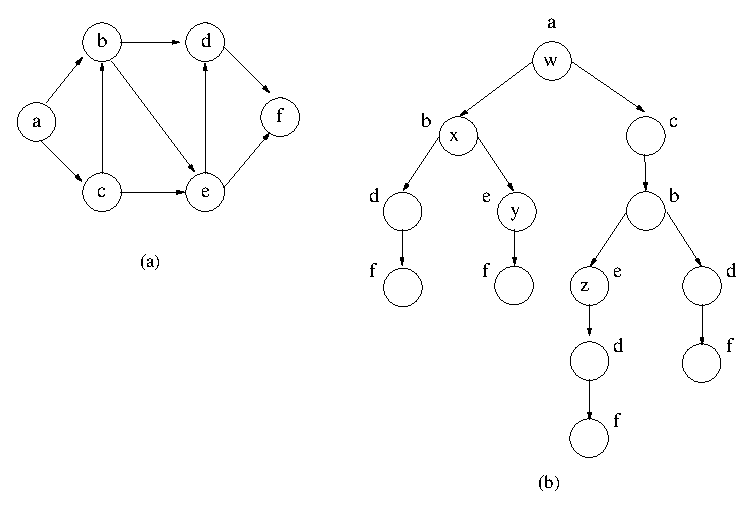
\includegraphics{./figs/prefixo.eps}
  \caption{\label{fig:prefixo} (b) mostra a �rvore dos prefixos dos
   caminhos
   $\seq{s,a,c,t}$,
   $\seq{s,a,d,t}$,
   $\seq{s,b,a,c,t}$ e 
   $\seq{s,b,a,d,c,t}$ no grafo em~(a).
  Na �rvore, um s�mbolo ao lado de um n\'o � o r\'otulo desse n\'o.
  Os r\'otulos dos arcos n�o est�o representados na figura. O s�mbolo 
  dentro de um n\'o � o seu nome.
  }
 \end{center}
 \end{figure}






\section{M�todo gen�rico}

A descri��o que fazemos �, de certa forma, \textit{top-down}. 
Come�aremos com um m�todo gen�rico que ser� refinado a cada passo incluindo,
convenientemente, algumas subrotinas auxiliares.
%%%%%%%%%%%%%%%%%%%%%%%%%%%%%%%%%%%%%%%%%%%%%%%%%%%%%%%%%%%%%%%%%%%%% 
O nosso interesse aqui � numa descri��o mais conceitual em que 
a corre��o e o consumo de tempo polinomial do m�todo sejam um tanto quanto
evidentes. 
%%%%%%%%%%%%%%%%%%%%%%%%%%%%%%%%%%%%%%%%%%%%%%%%%%%%%%%%%%%%%%%%%%%%%
N�o temos a inten��o de descrever um algoritmo com o menor consumo de tempo. 

O m�todo abaixo recebe um grafo $(V,A)$, uma fun��o custo, dois v�rtices $s$ e
$t$ e um inteiro positivo $k$ e devolve uma lista $\seq{P_1,\ldots,P_k}$ de
$k$-menores caminhos de $s$ a~$t$.

\begin{algoritmo}

\textbf{M�todo} \Generico{} $(V,A,c,s,t,k)$ %\\[2mm]
   
0\x $\Pcal \larr \mbox{conjunto dos caminhos de $s$ a~$t$}$ 

1\x \para{} $i=1,\ldots,k$ \faca %\\[1mm]

2\xx  $P_i \larr \mbox{caminho de custo m�nimo em $\Pcal$}$ %\\[1mm]

3\xx  $\Pcal \larr \Pcal - P_i$

4\x \devolva{} $\seq{P_1,\ldots,P_k}$

\end{algoritmo}

No in�cio de cada itera��o da linha~1 o conjunto $\Pcal$ cont�m os
candidatos a $i$-�simo caminho m�nimo de $s$ a~$t$. 
O m�todo de Yen � uma elabora��o do m�todo \Generico.
Em vez do conjunto 
$\Pcal$, Yen mant�m, pelo menos conceitualmente, uma parti��o
$\Pi$ de $\Pcal$.
Em cada itera��o, � escolhido o caminho mais barato
dentre um conjunto $\Lcal$ formado por \textit{um} caminho 
m�nimo $P_{\pi}$ representante de
cada parte $\pi$ de~$\Pi$ e depois a parti��o � atualizada. 

\begin{algoritmo}

\textbf{M�todo} \YenGenerico{} $(V,A,c,s,t,k)$ %\\[2mm]
   
0\x $\Pi \larr \{\{\mbox{conjunto dos caminhos de $s$ a~$t$}\}\}$

1\x $\Qcal \larr \emptyset $

2\x \para{} $i=1,\ldots,k$ \faca %\\[1mm]

3\xx  $\Lcal  \larr \seq{P_{\pi} : P_{\pi} \ \mbox{� caminho m�nimo da parte $\pi$
de~$\Pi$}}$

4\xx  $P_i \larr \mbox{caminho de custo m�nimo em $\Lcal$}$ %\\[1mm]

5\xx  $\Qcal \larr \Qcal \cup \{P_i\}$

6\xx  $\Pi \larr \AtualizeGenerico~(V,A,\Qcal)$

7\x \devolva{} $\seq{P_1,\ldots,P_k}$

\end{algoritmo}

Como veremos, a efici�ncia do m�todo de Yen depender� fortemente da estrutura
restrita dos caminhos nas partes de~$\Pi$: cada parte � formada por
caminhos que t�m um certo prefixo comum. 

Seja $\Pcal_{st}$ a cole��o
dos caminhos de $s$ a~$t$ em $(V,A)$.
Suponha que $\Qcal$ seja a lista de 
caminhos distintos de $s$ a~$t$ na linha~5 do m�todo
\YenGenerico{}.  Passamos a descrever a parti��o
$\Pi$ dos caminhos em $\Pcal := \Pcal_{st} \setminus \Qcal$.
Para isto � conveniente utilizarmos a 
\textit{�rvore dos prefixos} de
$\Qcal$, como foi feito por John Hershberger,
Matthew Maxel e Subhash Suri~\cite{hershberger:acmta-3-??}.

No que segue suponha que $(N,E,f)$ seja 
a �rvore dos prefixos de $\Qcal$ e $u$ seja um n\'o em $N$.
%%%%%%%%%%%%%%%%%%%%%%%%%%%%%%%%%%%%%%%%%%%%%%%%%%%%%%%%%
Representaremos por $R_u$\mar{$R_u$} o
caminho da raiz a $u$ na �rvore. Assim,  $f(R_u)$\mar{$f(R_u)$} �
o prefixo de um caminho em $\Qcal$. 
Por exemplo, na �rvore dos prefixos da figura~\ref{fig:prefixo}(b)
temos que $R_y = \seq{w,wx,x,xy,y}$ e $f(R_y) = \seq{s,sa,a,ad,d}$.

Seja\mar{$A_u$}
%$A_u$ a
%cole��o dos arcos em $A$ com ponta inicial em $f(u)$ e
%ponta final $f(w)$ para todo arco $uw$ em $E$, isto �,
\begin{eqnarray*}
A_u := \{ (f(u),f(w)) : uw \in E\}. 
\end{eqnarray*}  
e seja $\pi_u$\mar{$\pi_u$} o conjunto dos caminhos em $\Pcal$ com
prefixo $f(R_u)$ e que n�o possuem arcos em~$A_u$.
Para o exemplo na figura~\ref{fig:prefixo} temos que 
\begin{eqnarray*}
A_w = \{sa,sb\}, 
A_x = \{ac,ad\}, 
A_y = \{dt\} \ \mbox{e} \ 
A_z = \{dc\} \\
\pi_w = \emptyset, 
\pi_x = \emptyset,
\pi_y = \{\seq{s,a,d,c,t}\},  \ \mbox{e} \
\pi_z = \{\seq{s,b,a,d,t}\}.  
\end{eqnarray*}

A parti��o~$\Pi$\mar{$\Pi$} � formada por uma parte $\pi_u$ para
cada v�rtice $u$ em $N$, ou seja,
\[
\Pi := \{\pi_u : u \in N\}.
\]
No in�cio de cada itera��o da linha~2 o n�mero de partes � certamente n�o
superior a $n \times i$.
O algoritmo \AtualizeGenerico{} resume toda a discuss�o acima.


\begin{algoritmo}

\textbf{Algoritmo} \AtualizeGenerico{} $(V,A,\Qcal)$ %\\[2mm]
   
0\x $\Pi \larr \emptyset \quad \quad \Pcal \larr \Pcal_{st} \setminus \Qcal$

1\x $(N,E,f) \larr$ �rvore dos prefixos de $\Qcal$

2\x \para{} \cada{} $u \in N$ \faca %\\[1mm]

3\xx  $\pi_u \larr \{\mbox{caminhos em $\Pcal$ com prefixo $f(R_u)$}$

\xxxxx \quad e que n�o possuem arcos em $A_u \}$

4\xx  $\Pi \larr  \Pi \cup \{\pi_u\}$ %\\[1mm]

5\x \devolva{} $\Pi$

\end{algoritmo}

Podemos verificar que cada caminho em $\Qcal$ n�o pertence a
nenhuma parte de~$\Pi$. Tamb�m podemos verificar que cada
caminho $P$ em $\Pcal$ est� em uma �nica 
parte de~$\Pi$. De fato, seja $P'$ o maior prefixo de~$P$ 
que � prefixo de algum caminho em $\Qcal$. Pela defini��o
de �rvore de prefixos, existe um �nico caminho $R'$ em 
$(N,E)$ com in�cio na raiz e tal que $P' = f(R')$. 
Para o v�rtice $u$ t�rmino de $R'$ temos que $P$ est� em
$\pi_u$ e � a �nica parte que possui $P$. 

Desta forma, no in�cio de cada itera��o das linhas
2--6  do m�todo \YenGenerico{}, $\Pi$ � uma parti��o de
$\Pcal$, portanto a corre��o
do m�todo � evidente.


%% ???Ainda utilizando a estrutura da �rvore dos prefixos de  

As �rvores dos prefixos de duas
execu�\~oes consecutivas do algoritmo \AtualizeGenerico{} s�o
muito semelhantes: apenas um novo caminho � acrescentado �
�rvore anterior.  Isto, em particular, significa que as
parti�\~oes de duas itera�\~oes consecutivas das linhas 2--6 do
m�todo \YenGenerico{} s�o muitos semelhantes. Esta
observa��o pode ser utilizada para o algoritmo
\AtualizeGenerico{} obter mais eficientemente
uma parti��o a partir da parti��o anterior.
 





\section{M�todo de Yen}

O m�todo que Jin Y. Yen~\cite{yen:ms-17-712} desenvolveu para resolver
o \kCM{} parece ter um papel central entre os algoritmos que foram
posteriormente projetados para o \kCM\ ou mesmo para vers\~oes mais
restritas do
problema~\cite{eppstein:siamjc-28-652,katoh:n-12-411,hershberger:acmta-3-??}.
V�rias melhorias pr�ticas do m�todo de Yen t�m sido implementadas e
testadas~\cite{brander:370,eleni:n-34-88,martins:qjbfiors-1-121,martins:relatorio,perko:n-16-149}

Antes de prosseguirmos, mencionamos que o m�todo de Yen foi generalizado por
Eugene L. Lawler~\cite{lawler:ms-18-401} para problemas de otimiza��o
combinat\'oria, contanto que seja fornecida uma subrotina para determinar uma
solu��o \'otima sujeita a condi��o de que certas vari�veis t�m seus valores
fixados. Por exemplo, no caso do m�todo de Yen para o \kCM{} essa subrotina
resolve o seguinte \defi{problema do sub-caminho m�nimo}\index{problema!do
sub-caminho m�nimo@do sub-caminhos m�nimo}, denotado por \PSM:
 \begin{quote}
   \textbf{Problema} \PSM$(V,A,c,s,t,P,F)$:%
   \index{PSM@\PSM}\mar{\PSM}
   %%%%%%%%%%%%%%%%%%%%%%%%%%%%%%%%%%%%%%%%%%%%%%%%%%%%%%%%%%%%%%%%%%%
   Dado um grafo $(V,A)$, uma fun��o
   custo $c$, dois v�rtice $s$ e $t$, um caminho $P$ e uma parte $F$ de $A$, 
   encontrar um caminho de custo m�nimo 
   de $s$ a~$t$ que tem $P$ como prefixo e n�o cont�m arcos em $F$.
 \end{quote}
\'E evidente que se $P$ n�o tem in�cio em $s$ ent�o o problema �
invi�vel. Do ponto de vista de m�todo Lawler, o prefixo $P$ e o conjunto $F$
s�o as `vari�veis' com valores fixados. 
 
Resolver o \PCM$(V,A,c,s,t)$ � o mesmo que resolver
\PSM$(V,A,c,s,t,\seq{s},\emptyset)$.  Por outro lado, o
\PSM{} pode ser solucionado aplicando-se um algoritmo para o
\PCM{} em um sub-grafo apropriado de $(V,A)$.  Desta forma, o
\PCM{} e o \PSM{} s�o computacionalmente equivalentes e
podem ser resolvidos em tempo $T(n,m)$.


Conceitualmente, o m�todo de Yen � uma elabora��o do m�todo \YenGenerico.
No in�cio de cada itera��o da linha~2, $\Lcal$ � uma lista dos
candidatos a $i$-�simo caminho m�nimo de $s$ a~$t$. 
Ao inv�s da parti��o  $\Pi$ 
de $\Pcal$, Yen mant�m em $\Lcal$ um caminho m�nimo de
cada parte de $\Pi$. 
%%%%%%%%%%%%%%%%%%%%%%%%%%%%%%%%%%%%%%%%%%%%%%%%%%%%%%%%%%%%%%%%%
%de $\Pcal$ em n�o mais do que $2i$ partes e uma lista $L$ com 
%um caminho mais barato de cada uma das partes. 
Em cada itera��o � escolhido  o caminho mais barato entre 
todos em $\Lcal$  e a parti��o � \textit{levemente} atualizada.

\begin{algoritmo}

\textbf{M�todo} \Yen{} $(V,A,c,s,t,k)$ %\\[2mm]
   

1\x $\Lcal \larr \{ \mbox{um caminho de custo m�nimo de $s$ a $t$} \}$

2\x $\Qcal \larr \emptyset$

3\x \para{} $i=1,\ldots,k$ \faca %\\[1mm]

4\xx  $P_i \larr \mbox{caminho de custo m�nimo em $\Lcal$}$
%\\[1mm]

%4\xx  $\Lcal \larr \Lcal \setminus \{P_i\}$

5\xx  $\Qcal \larr \Qcal \cup \{P_i\}$

6\xx  $\Lcal \larr \Atualize~(V,A,c,\Qcal)$

7\x \devolva{} $\seq{P_1,\ldots,P_k}$

\end{algoritmo}


%%Na verdade, com o n�mero dos caminhos em $\Pcal$ � muito grande


\begin{algoritmo}

\textbf{Algoritmo} \Atualize{} $(V,A,c,\Qcal)$ %\\[2mm]
   
0\x $\Lcal \larr \emptyset$

1\x $(N,E,f) \larr$ �rvore dos prefixos de $\Qcal$

2\x \para{} \cada{} $u \in N$ \faca %\\[1mm]

3\xx  $P_u \larr \mbox{caminho de $s$ a~$t$ de custo m�nimo com prefixo $f(R_u)$}$

\xxxxx e que n�o possui arcos em $A_u$

4\xx  $\Lcal \larr  \Lcal \cup \{P_u\}$ %\\[1mm]

5\x \devolva{} $\Lcal$


\end{algoritmo}


Na linha~3 do algoritmo \Atualize{}, na verdade, 
estamos resolvendo 
o problema \PSM $(V,A,c,s,t,f(R_u),A_u)$. Assim, o consumo de tempo do
  algoritmo resultante � $n \, i \, T(n,m))$. Em chamadas consecutivas do
  algoritmo \Atualize{}, as �rvores dos prefixos calculadas s�o muito
  semelhantes.
%Logo, � poss�vel fazermos com que o consumo de tempo seja $n \, T(n,m)$.
De fato, o algoritmo  pode ser implementado de tal maneira
que o consumo o seu consumo de tempo seja $n \, T(n,m)$.

O m�todo de \Yen{} pode ser implementado de tal maneira que o seu consumo de
tempo seja proporcional a $k \, n \, T(n,m)$.




%%%%%%%%%%%%%%%%%%%%%%%%%%%%%%%%%%%%%%%%%%%%%%%%%%%%%%%%%%%%%%%%%%%%%%%%%%%%
%%
%%  CAP�TULO. M�TODO DE YEN
%%
%%%%%%%%%%%%%%%%%%%%%%%%%%%%%%%%%%%%%%%%%%%%%%%%%%%%%%%%%%%%%%%%%%%%%%%%%%%% 
\chapter{Algoritmo de Katoh, Ibaraki e Mine}
\label{cap:algoritmo-kim}

Neste cap�tulo trataremos, propriamente dito, do algoritmo desenvolvido por Katoh, Ibaraki e Mine, o qual chamaremos de \KIM.
Para entend�-lo fizemos usos de v�rios artigos diferentes. 
Come�amos pelo artigo original de Naoki Katoh,
Toshihide Ibaraki e H. Mine~\cite{katoh:n-12-411} (KIM), sob o qual a implementa��o foi feita.
O artigo � bem preciso do ponto de vista da implementa��o, trabalhando com �ndices e citando at� estruturas 
para implementa��o. 
Entretanto, em se tratando do entendimento em termos gerais n�o ajudou muito.

Uma vez que o artigo de Jin Y. Yen~\cite{yen:ms-17-712} fora citado pelo  de KIM, achamos que seria de grande utilidade 
l�-lo. 
Al�m do mais, sabemos que o algoritmo \KIM{} � uma melhoria do  \Yen{}, sendo espec�fico para grafos sim�tricos.
Ap�s a leitura do artigo de Yen, 
come�amos a vislumbrar melhor o algoritmo \KIM{} e a entend�-lo com mais propriedade.

Em seguida, encontramos o artigo de John Hershberger, Matthew Maxel e Subhash Suri~\cite{hershberger:acmta-3-??}, 
o qual foi muito elucidativo. 
Este trata de uma extens�o da id�ia central do algoritmo \KIM{} 
para grafos. 
O que mais nos chamou a aten��o foi a maneira como o algoritmo foi descrito.
Os autores procuraram trabalhar com id�ias mais gerais e lidar com estruturas mais sofisticadas, deixando de lado
a quantidade exorbitante de �ndices e descri��es de baixo n�vel apresentadas no artigo de KIM.

Finalmente, vale citar o artigo de Eleni Hadjiconstantinou e Nicos Christofides~\cite{eleni:n-34-88} que 
trata de uma implementa��o do algoritmo \KIM{} utilizando algumas mudan�as que levam a um melhor desempenho na pr�tica.
Neste artigo, a descri��o do algoritmo � feita com mais clareza, raz�o pela qual decidimos cit�-lo aqui. 

Nosso plano � apresentar o algoritmo  \KIM{}, bem como suas subrotinas e principais id�ias, comentando sobre 
o desempenho assint�tico das principais rotinas, em seguida exibiremos uma simula��o e finalizaremos
exibindo pontos importantes sobre a nossa implementa��o.

\section{Vis�o Geral}

O algoritmo \KIM{} �, de certa forma, uma vers�o do algoritmo \Yen{} espec�fica para grafos sim�tricos.
Mais especificamente, o algoritmo \HMS{} apresentado no cap�tulo~\ref{cap:hershberger}, pode ser visto
como a aplica��o de algumas das id�ias do algoritmo \KIM{} � grafos.
O algoritmo \KIM{} aplica uma t�cnica mais fina de particionamento de caminhos, semelhante � 
apresentada no cap�tulo~\ref{cap:hershberger}, sendo que o n�mero de parti��es � sempre menor
a $3 \times |Q|$, onde $|Q|$ � a quantidade de caminhos calculados at� um dado momento da execu��o, e a quantidade de 
caminhos candidatos � sempre menor ou igual a $2 \times |Q|-1$.
Em cada itera��o, no m�ximo, tr�s novos caminhos s�o gerados e adicionados � lista de caminhos candidatos,
sendo que na itera��o seguinte, um de menor custo � selecionado.

Seja $(V,A,c)$ um grafo sim�trico com uma fun��o custo definida, $s$ e $t$ dois v�rtices distintos,
$k$ um inteiro positivo representando a quantidade de caminhos que se deseja calcular entre $s$ e $t$.
O algoritmo \KIM{}, inicialmente, calcula um caminho de custo m�nimo entre $s$ e $t$ usando algum algoritmo que
resolva o problema \PCM{}~(\ref{prob:pcm}).
Em seguida, gera um caminho de custo m�nimo que desvia do anterior em algum de seus v�rtices, utilizando para
tal uma subrotina que resolve o problema do desvio m�nimo~(\ref{prob:pdm}).
A partir dos dois caminhos gerados at� o momento, o conjunto $\Pcal_{st}$ � particionado em tr�s: $P_{a}$, $P_{b}$ e $P_{c}$.
Um caminho de menor custo de cada uma das parti��es, seu representante, 
� gerado e adicionado � lista de caminhos candidatos $\Lcal$.
A gera��o de cada representante utiliza como subrotina um algoritmo para o problema do desvio m�nimo restrito~(\ref{prob:pdmr}).
Um caminho de menor custo � retirado da lista de caminhos candidatos tornando-se o $P_3$.
A partir de $P_3$ e seu pai, geramos, no m�ximo, mais tr�s caminhos candidatos, cada qual representante
de um das parti��es $P_a,P_b$ e $P_c$ definidas por $P_3$ e seu pai.
Na se��o~\ref{sec:particoes}, as parti��es ser�o apresentadas com mais detalhes.
O processo continua at� que o $k$-�simo menor caminho seja retirado da lista $\Lcal$ ou n�o haja mais caminhos em $\Lcal$.
%% O caminho de menor custo � retirado da lista de caminhos candidatos $\Lcal$ e, a partir dele, o conjunto $\Pcal_{st}$ � particionado, 
%% em seis parti��es, $P_{a_2},P_{b_2},P_{c_2},P_{a_3},P_{b_3}$ e $P_{c_3}$.
%% Cada um dos representantes das parti��es $P_{a_3},P_{b_3},P_{c_3}$ � adicionado � lista $\Lcal$ e o processo continua at� que o $k-$�simo 
%% caminho de menor custo seja retirado de $\Lcal$, ou n�o exista mais nenhum caminho em $\Lcal$.

%% Sejam $s$ e $t$ os v�rtices de origem e destino, $(V,A,c)$ um grafo sim�trico com uma fun��o custo
%%  definida e $k$ a quantidade de caminhos que se deseja gerar entre $s$ e $t$, o algoritmo \KIM{}
%%  gera o $i-$�simo caminho $P_i$, $2 < i \leq k$, particionando os caminhos previamente calculados $\seq{P_1,P_2,\ldots,P_{i-1}}$
%% em, no m�ximo, tr�s parti��es: $P_a,P_b$ e $P_c$. 
%% Por ora, uma parti��o ser� descrita por um grafo $(V^{'},A^{'})\subseteq (V,A)$, mas a seguir explicitaremos 
%% as altera��es no grafo requeridas para a gera��o de um caminho em cada parti��o.
%% Um caminho de custo m�nimo, diferente dos caminhos $\seq{P_1,P_2,\ldots,P_{i-1}}$, � gerado em cada parti��o, atrav�s
%% do algoritmo \FSP{}. 
%% Esses caminhos s�o ent�o adicionados � lista de caminhos candidatos $\Lcal$.
%% Retira-se ent�o o caminho de custo m�nimo em $\Lcal$, o qual se tornar� o $i-$�simo caminho.
%% O procedimento � repetido at� que o $k-$�simo caminho tenha sido gerado ou n�o haja mais caminhos em $\Lcal$.

A seguir apresentamos a rotina principal do algoritmo \KIM{}, de certa forma semelhante a do \Yen{}.

\begin{algoritmo}

\textbf{Algoritmo} \KIM{} $(V,A,c,s,t,k)$ %\\[2mm]%
\index{algoritmo!KIM@\KIM}\index{KIM@\KIM} 

1\x $P_1 \larr $ um caminho de custo m�nimo de $s$ a $t$

2\x $P_2 \larr \FSP~(V,A,c,P_1,s,t)$

2\x $\Lcal \larr P_2$

3\x $\Qcal \larr P_1 $

4\x \para{} $i=2,\ldots,k$ \faca %\\[1mm]

5\xx  $P_i \larr \mbox{caminho de custo m�nimo em $\Lcal$}$
%\\[1mm]

%4\xx  $\Lcal \larr \Lcal \setminus \{P_i\}$

6\xx  $\Qcal \larr \Qcal \cup \{P_i\}$

7\xx  $\Lcal \larr \AtualizeKIM~(V,A,c,\Qcal,P,\Lcal)$

8\x \devolva{} $\seq{P_1,\ldots,P_k}$

\end{algoritmo}

Na rotina \AtualizeKIM, o conjunto dos caminhos candidatos � incrementado de, no m�ximo, tr�s caminhos,
cada qual representante de uma das parti��es: $P_a,P_b$ e $P_c$.

\begin{algoritmo}

\textbf{Algoritmo} \AtualizeKIM{} $(V,A,c,\Qcal,P,\Lcal)$ %\\[2mm]
\index{algoritmo!AtualizeKIM@\AtualizeKIM}\index{AtualizeKIM@\AtualizeKIM}

1\x $P_a \larr \Pa(V,A,c,\Qcal,P)$

2\x $P_b \larr \Pb(V,A,c,\Qcal,P)$

3\x $P_c \larr \Pc(V,A,c,\Qcal,P)$

4\x $\Lcal \larr \Lcal \cup \{P_a,P_b,P_c\}$

5\x \devolva{} $\Lcal$
\end{algoritmo}


\section{Problema do desvio m�nimo}

Na se��o~\ref{prob:pdm} o problema do desvio m�nimo foi apresentado e no cap�tulo~\ref{cap:hershberger}
uma heur�stica foi proposta.
Essa heur�stica � bastante semelhante a que iremos apresentar, no entanto o faremos de uma maneira um pouco diferente.

Nesta se��o mostraremos como o problema do desvio m�nimo � resolvido pelo algoritmo \KIM.
O plano desta se��o � apresentar cada um dos elementos que fazem parte da solu��o do problema \PDM, pelo algoritmo \KIM{}.
Come�aremos pelas �rvores de menores caminhos, apresentadas no cap�tulo~\ref{cap:hershberger} como arboresc�ncias 
com fun��es potenciais.
Em seguida, mostraremos como caminhos de custos m�nimos podem ser gerados a partir destas �rvores.
Prosseguiremos explicando um m�todo de rotula��o dos n�s dessas �rvores, o qual ser� empregado
na obten��o de um desvio m�nimo.
Exibiremos um caso espec�fico em que a solu��o n�o funciona.
Trataremos brevemente do desvio m�nimo restrito, o qual est�, de fato, no algoritmo \KIM{}.
Finalizaremos, utilizando as �rvores rotuladas na solu��o do problema do desvio m�nimo.

\subsection*{�rvores de menores caminhos $T_s$ e $T_t$}

Seja $(V,A,c)$ um grafo sim�trico com uma fun��o custo $c$ nas arestas e $v$ um de seus v�rtices.
Uma �rvore de menores caminhos com raiz em $v$ � uma arboresc�ncia com raiz $v$ formada pelos
caminhos de menores custos de $v$ a cada um dos seus v�rtices acess�veis.
Cada v�rtice acess�vel possui um potencial que � igual ao custo de um caminho de custo m�nimo a partir de $v$.
Na figura a seguir temos um grafo e duas �rvores de menores custos, uma com raiz em $s$ e outra em $t$.

\begin{figure}[htb]
			\tikzstyle{vertex}=[circle,fill=black!25,minimum size=15pt,inner sep=0pt]
			\tikzstyle{start} = [vertex, fill=red!24]
			\tikzstyle{end} = [vertex, fill=red!24]
			\tikzstyle{edge} = [draw,thick,-]
			\tikzstyle{weight} = [font=\tiny]
			\tikzstyle{selected edge} = [draw,line width=2pt,-,red!50]
			\tikzstyle{not used} = [draw,line width=2pt,-,blue!50]

			\tikzstyle{node}=[circle,fill=black!25,minimum size=10pt,inner sep=0pt]
			\tikzstyle{root} = [node, fill=red!24]
			\tikzstyle{leaf} = [node, fill=gray!24]
			\tikzstyle{onPath} = [node, fill=red!24]
			\tikzstyle{edge} = [draw,thick,-]
			\tikzstyle{weight} = [font=\tiny]
			\tikzstyle{selected edge} = [draw,thick,-,red!50]
			%\tikzstyle{LabelStyle}=[fill=white,sloped]
			
			% Set the overall layout of the tree
		\tikzstyle{level 1}=[level distance=1.5cm, sibling distance=2.5cm]
		\tikzstyle{level 2}=[level distance=1.5cm, sibling distance=2.5cm]

	\begin{tikzpicture}[scale=1.0]
        \node[start] (a) {s};
        \node[vertex] (b) [right of=a,node distance=2cm] {b};
        \node[vertex] (c) [above right of=b,node distance=2cm] {c};
        \node[vertex] (d) [right of=b,node distance=2cm] {d};
        \node[vertex] (f) [below right of=b,node distance=2cm] {f};
        \node[end] (e) [right of=d,node distance=2cm] {t};
          
         \path[edge] (a) -- node[weight,above] {$1$} (b);
         \path[edge] (b) -- node[weight,above] {$1$} (d);
         \path[edge] (d) -- node[weight,above] {$1$} (e);
         \path[edge] (a) -- node[weight,above] {$10$} (c);
         \path[edge] (b) -- node[weight,above] {$10$} (c);
         \path[edge] (c) -- node[weight,above] {$1$} (d);
         \path[edge] (b) -- node[weight,above] {$1$} (f);
         \path[edge] (f) -- node[weight,above] {$1$} (d);


  	\node[root,right of=c,node distance=5cm] (ra) {s} [grow=down,-] 
  	    child {
				node[node] (ab) {b}
				child[grow=south west]{
						node[node] (abd){d} 
						child[grow=south west]{
							node[node] (abde) {t}
							edge from parent
							node[left,weight] {1}
						}
						child[grow=south east] {
							node[node] (abdc) {c}
							edge from parent
							node[right,weight] {1}
	 					}
						edge from parent
						node[left,weight] {1}
				}
				child[grow=south east]{
					node[node] {f} 
					edge from parent
					node[left,weight] {1}
				}				
				edge from parent
				node[left,weight] {1}
	 };
	  \node[root,right of=abdc,node distance=4cm] (e) {t} [grow=up,-] 
  	    child {
				node[node]  (ed) {d} 
				child[grow=north west]{
						node[node] (edb) {b}  
						child{
							node[node] (edba) {s} 
							edge from parent
							node[left,weight] {1}
						}
						edge from parent
						node[left,weight] {1}
				}
				child {
							node[node] {c}
							edge from parent
							node[left,weight] {1}
	 					}
				child[grow=north east] {
							node[node] {f}
							edge from parent
							node[left,weight] {1}
	 					}
				edge from parent
				node[left,weight] {1}
	 };
	\end{tikzpicture}
\caption{Exemplos de �rvores de menores caminhos}	
\end{figure}

Observe que cada v�rtice � acessado por um caminho de custo m�nimo a partir da raiz.
Por exemplo: na �rvore com raiz em $a$ o v�rtice $c$ � acessado pelo caminho $\seq{a,b,d,c}$ de custo 3.

\subsection*{Desvios m�nimos}
Na se��o~\label{prob:pcm} o problema do desvio m�nimo foi apresentado.
Apenas relembrando, o problema do desvio m�nimo consiste em, 
dado um caminho de custo m�nimo, encontrar um caminho diferente, com mesma ponta inicial e 
com custo m�nimo.
Na figura a seguir vemos inicialmente um caminho de $s$ a $t$.
\tikzstyle{vertex}=[circle,fill=black!25,minimum size=15pt,inner sep=0pt]
\tikzstyle{start} = [vertex, fill=red!24]
\tikzstyle{end} = [vertex, fill=red!24]
\tikzstyle{edge} = [draw,thick,-]
\tikzstyle{weight} = [font=\tiny]
\tikzstyle{selected edge} = [draw,line width=2pt,-,red!50]
\tikzstyle{not used} = [draw,line width=2pt,-,blue!50]

	\begin{tikzpicture}[scale=1.0, auto,swap,node distance=7cm]
        \node[start] (s) {s};
        \node[end] (t) [right of=s] {t};
        \node [right of=t, node distance=1cm] {P};
        
         \path[selected edge] (s) -- node[weight] {} (t);
        
   \end{tikzpicture}

Um desvio m�nimo de $P$ corresponde a um caminho de custo m�nimo entre $s$ a $t$, diferente de $P$.
na figura a seguir vemos o desvio m�nimo $D$, que corresponde ao caminho que tem o prefixo comum $\seq{s,\ldots,\delta}$,
tornando-se diferente de $P$ a partir da�.

	\begin{tikzpicture}[scale=1.0, auto,swap,node distance=2cm]
        \node[start] (s) {s};
        \node[vertex] (desvio) [right of=s] {$\delta$};
        \node[vertex] (u) [below right of=desvio] {u};
        \node (aux) [right of=u] {...};       
        \node[end,node distance=5cm] (t) [right of=desvio] {t};
        \node[end] (t2) [right of=aux] {t};
        \node  [right of=t, node distance=1cm] {P};
        \node  [right of=t2, node distance=1cm] {D};
         \path[selected edge,dashed] (s) -- node[weight] {} (desvio);
         \path[selected edge] (desvio) -- node[weight] {} (t);
         \path[not used] (desvio) -- node[weight] {} (u);
         \path[edge,dashed] (u) -- node[weight,dashed] {} (aux);
         \path[edge,dashed] (aux) -- node[weight,dashed] {} (t2);
         
   \end{tikzpicture}

Na se��o anterior vimos as �rvores de menores caminhos. 
Agora iremos utiliz�-las na constru��o de desvios m�nimos.

Seja $T_s$ uma �rvore de menores caminhos com origem em $s$, 
$T_t$ uma �rvore de menores caminhos com raiz em $t$,
$P$ um caminho de custo m�nimo entre $s$ e $t$ tal que $P \in T_s$ e $P \in T_t$.
Suponha que exista um desvio m�nimo $D$ de $P$.
Sendo $D$ um desvio m�nimo de $P$, compartilha com este um prefixo maximal: $\seq{s,\ldots,\delta}$,
para algum v�rtice $\delta \in P$.
Seja $u$ o v�rtice seguinte a $\delta$ no caminho $D$.
Naturalmente $\delta u \notin P$.
Sendo assim, temos duas op��es para a aresta $\delta u$:
	\begin{itemize}
	\item $\delta u \in T_s$ \\
		Neste caso, o caminho $D$ corresponde ao formado pela concatena��o do caminho de $s$ a $u$ na �rvore $T_s$		
		ao caminho de $u$ a $t$ na �rvore $T_s$. 
		Observe que $u \in T_s$, pois � acess�vel a partir de $s$. Al�m disso, como $\delta u \in T_s$, 
		temos que o caminho de $s$ a $u$ pertence a $T_s$.
		Pela defini��o de �rvores de menores caminhos, o caminho de $u$ a $t$ em $T_t$ � de custo m�nimo.
		Sendo assim, $D = s \underset{T_s}{\longrightarrow} u \underset{T_t}{\longrightarrow} t$.
%% 		\begin{itemize}
%% 		\item $s \underset{T_s}{\longrightarrow} u \underset{T_t}{\longrightarrow} t$
%% 		\end{itemize}
	\item $\delta u \notin T_s$ \\
		Neste caso, podemos afirmar que o caminho de $s$ a $\delta$ concatenado � aresta $\delta u$ � um caminho de custo m�nimo de 
		$s$ a $u$, pois sendo $D$ um caminho de custo m�nimo, qualquer de seus prefixos deve ser de custo m�nimo.
		Como $u$ � acess�vel a partir de $t$ e sabendo que o caminho de $u$ a $t$ em $T_t$ � de custo m�nimo, temos que:
		$D = s \underset{T_s}{\longrightarrow} u \underset{\in A}{\rightarrow} v \underset{T_t}{\longrightarrow} t$.
%% 		\begin{itemize}
%% 			\item $s \underset{T_s}{\longrightarrow} u \underset{\in A}{\rightarrow} v \underset{T_t}{\longrightarrow} t$
%% 		\end{itemize}

	\end{itemize}
Formalizaremos esses dois casos em dois tipos de caminhos na se��o seguinte.



\subsection*{Tipos de caminhos}

Seja $(V,A,c)$ um grafo sim�trico com uma fun��o custo definida em suas arestas,
$s$ e $t$ dois v�rtices distintos de $V$,
$T_s$ uma �rvore de menores caminhos com raiz em $s$,
$T_t$ uma �rvore de menores caminhos com raiz em $t$,
$P$ um caminho de custo m�nimo de $s$ a $t$,
$P_r$ o reverso de $P$,
$P \in T_s$ e $P_r \in T_t$.
Um desvio m�nimo constru�do atrav�s de $u \in V$ � de um dos dois tipos definidos a seguir:
\begin{description}
\item[\defi{Tipo I}]: $s \underset{T_s}{\longrightarrow} u \underset{T_t}{\longrightarrow} t$.  \mar{Tipo I} %Se $\epsilon(u)<\zeta(u)$ 
\newline
\item[\defi{Tipo II}]: $s \underset{T_s}{\longrightarrow} u \underset{\in A}{\rightarrow} v \underset{T_t}{\longrightarrow} t$. \mar{Tipo II} %Se $\epsilon(u)=\zeta(u)$ e $\epsilon(u)<\zeta(v)$
\end{description}

Na figura a seguir temos um grafo sim�trico, um caminho de custo m�nimo de $s$ a $t$: $\seq{s,b,d,t}$,
uma �rvore de menores caminhos com raiz em $s$ e outra em $t$, tal que $\seq{s,b,d,t} \in T_s$ e $\seq{t,d,b,s} \in T_t$.\\

\begin{figure}[htb]
			\tikzstyle{vertex}=[circle,fill=black!25,minimum size=15pt,inner sep=0pt]
			\tikzstyle{start} = [vertex, fill=red!24]
			\tikzstyle{end} = [vertex, fill=red!24]
			\tikzstyle{edge} = [draw,thick,-]
			\tikzstyle{weight} = [font=\tiny]
			\tikzstyle{selected edge} = [draw,line width=2pt,-,red!50]
			\tikzstyle{not used} = [draw,line width=2pt,-,blue!50]

			\tikzstyle{node}=[circle,fill=black!25,minimum size=10pt,inner sep=0pt]
			\tikzstyle{root} = [node, fill=red!24]
			\tikzstyle{leaf} = [node, fill=gray!24]
			\tikzstyle{onPath} = [node, fill=red!24]
			\tikzstyle{edge} = [draw,thick,-]
			\tikzstyle{weight} = [font=\tiny]
			\tikzstyle{selected edge} = [draw,thick,-,red!50]
			%\tikzstyle{LabelStyle}=[fill=white,sloped]
			
			% Set the overall layout of the tree
		\tikzstyle{level 1}=[level distance=1.5cm, sibling distance=2.5cm]
		\tikzstyle{level 2}=[level distance=1.5cm, sibling distance=2.5cm]

	\begin{tikzpicture}[scale=1.0]
        \node[start] (a) {s};
        \node[vertex] (b) [right of=a,node distance=2cm] {b};
        \node[vertex] (c) [above right of=b,node distance=2cm] {c};
        \node[vertex] (d) [right of=b,node distance=2cm] {d};
        \node[vertex] (f) [below right of=b,node distance=2cm] {f};
        \node[end] (e) [right of=d,node distance=2cm] {t};
          
         \path[edge] (a) -- node[weight,above] {$1$} (b);
         \path[edge] (b) -- node[weight,above] {$1$} (d);
         \path[edge] (d) -- node[weight,above] {$1$} (e);
         \path[edge] (a) -- node[weight,above] {$10$} (c);
         \path[edge] (b) -- node[weight,above] {$10$} (c);
         \path[edge] (c) -- node[weight,above] {$1$} (d);
         \path[edge] (b) -- node[weight,above] {$1$} (f);
         \path[edge] (f) -- node[weight,above] {$1$} (d);

		 	\path[selected edge] (a) -- node[weight] {} (b);
		   \path[selected edge] (b) -- node[weight] {} (d);
		   \path[selected edge] (d) -- node[weight] {} (e);


  	\node[root,right of=c,node distance=5cm] (ra) {s} [grow=down,-] 
  	    child {
				node[node] (ab) {b}
				child[grow=south west]{
						node[node] (abd){d} 
						child[grow=south west]{
							node[node] (abde) {t}
							edge from parent
							node[left,weight] {1}
						}
						child[grow=south east] {
							node[node] (abdc) {c}
							edge from parent
							node[right,weight] {1}
	 					}
						edge from parent
						node[left,weight] {1}
				}
				child[grow=south east]{
					node[node] (abf) {f} 
					edge from parent
					node[left,weight] {1}
				}				
				edge from parent
				node[left,weight] {1}
	 };
	   	\path[selected edge] (ra) -- node[weight] {} (ab);
			\path[selected edge] (ab) -- node[weight] {} (abd);
		   \path[selected edge] (abd) -- node[weight] {} (abde);   

	  \node[root,right of=abdc,node distance=4cm] (re) {t} [grow=up,-] 
  	    child {
				node[node]  (ed) {d} 
				child[grow=north east]{
						node[node] (edb) {b}  
						child{
							node[node] (edba) {s} 
							edge from parent
							node[left,weight] {1}
						}
						edge from parent
						node[left,weight] {1}
				}
				child {
							node[node] (tdc) {c}
							edge from parent
							node[left,weight] {1}
	 					}
				child[grow=north west] {
							node[node] (tdf) {f}
							edge from parent
							node[left,weight] {1}
	 					}
				edge from parent
				node[left,weight] {1}
	 };
	  	\path[selected edge] (re) -- node[weight] {} (ed);
		\path[selected edge] (ed) -- node[weight] {} (edb);
   	\path[selected edge] (edb) -- node[weight] {} (edba);


   	\path[dashed,red] (abf) edge (tdf);
	 	\path[dashed,blue,bend left] (ab) edge (tdc);

	\end{tikzpicture}
\caption{Exemplos de caminhos \defi{tipo I} e \defi{tipo II}}	
\end{figure}

Em \textcolor{red}{vermelho}, temos o caminho \textcolor{red}{$\seq{s,b,f,d,t}$} do \defi{tipo I}:
$s \underset{T_s}{\longrightarrow} f \underset{T_t}{\longrightarrow} t$.
Em \textcolor{blue}{azul}, temos caminho \textcolor{blue}{$\seq{s,b,c,d,t}$} do \defi{tipo II}:
$s \underset{T_s}{\longrightarrow} b \underset{\in A}{\rightarrow} c \underset{T_t}{\longrightarrow} t$.\\
O desvio m�nimo de $\seq{s,b,d,t}$ corresponde ao caminho de custo m�nimo \textcolor{blue}{$\seq{s,b,c,d,t}$}.


\subsection*{Rotula��o das �rvores}
\label{sec:rotulacao}

Apresentaremos uma rotula��o de �rvores de menores caminhos que ser� utilizada em seguida para
gera��o eficiente de desvios m�nimos.

Seja $(V,A,c)$ um grafo sim�trico com uma fun��o custo definida em suas arestas,
$s$ e $t$ dois v�rtices distintos de $V$,
$T_s$ uma �rvore de menores caminhos com raiz em $s$,
$T_t$ uma �rvore de menores caminhos com raiz em $t$,
$P$ um caminho de custo m�nimo de $s$ a $t$,
$P_r$ o reverso de $P$,
$P \in T_s$ e $P_r \in T_t$.

Para as rotula��es utilizamos a fun��o-predecessor apresentada na se��o~\ref{sec:predecessor}.

Rotularemos os v�rtices de $T_s$ utilizando a \defi{rotula��o $\epsilon$} definida por: \mar{rotula��o $\epsilon$}
\begin{enumerate}[(1)]
\item $\epsilon(s)=1$ 
\item $u \neq s$
	\begin{itemize}
	\item Se $u \in P$ ent�o $\epsilon(u)=\epsilon(\pred_{T_s}(u))+1$
	\item Se $u \notin P$ ent�o $\epsilon(u)=\epsilon(\pred_{T_s}(u))$
	\end{itemize}
\end{enumerate}

Rotularemos os v�rtices de $T_t$ utilizando a \defi{rotula��o $\zeta$} definida por: \mar{rotula��o $\zeta$}
\begin{enumerate}[(1)]
\item $\zeta(t)=|P|$ 
\item $u \neq t$
	\begin{itemize}
	\item Se $u \in P$ ent�o $\zeta(u)=\zeta(\pred_{T_t}(u))-1$ 
	\item Se $u \notin P$ ent�o $\zeta(u)=\zeta(\pred_{T_t}(u))$
	\end{itemize}
\end{enumerate}

Pelas defini��es acima podemos perceber que $\forall u \in P$ temos $\epsilon(u)=\zeta(u)$.

Na figura a seguir, temos o caminho destacado \textcolor{red!50}{$\seq{s,b,d,t}$} e as rotula��es $\epsilon$ e $\zeta$ 
das �rvores de menores caminhos $T_s$ e $T_t$.
\begin{figure}[hbt]
			\tikzstyle{vertex}=[circle,fill=black!25,minimum size=15pt,inner sep=0pt]
			\tikzstyle{start} = [vertex, fill=red!24]
			\tikzstyle{end} = [vertex, fill=red!24]
			\tikzstyle{edge} = [draw,thick,-]
			\tikzstyle{weight} = [font=\tiny]
			\tikzstyle{selected edge} = [draw,line width=2pt,-,red!50]
			\tikzstyle{not used} = [draw,line width=2pt,-,blue!50]

			\tikzstyle{node}=[circle,fill=black!25,minimum size=10pt,inner sep=0pt]
			\tikzstyle{root} = [node, fill=red!24]
			\tikzstyle{leaf} = [node, fill=gray!24]
			\tikzstyle{onPath} = [node, fill=red!24]
			\tikzstyle{edge} = [draw,thick,-]
			\tikzstyle{weight} = [font=\tiny]
			\tikzstyle{selected edge} = [draw,thick,-,red!50]
			%\tikzstyle{LabelStyle}=[fill=white,sloped]
			
			% Set the overall layout of the tree
		\tikzstyle{level 1}=[level distance=1.5cm, sibling distance=2.5cm]
		\tikzstyle{level 2}=[level distance=1.5cm, sibling distance=2.5cm]

	\begin{tikzpicture}[scale=1.0]
  	\node[root,right of=c,node distance=5cm,label=right:{\footnotesize $\epsilon=1$}] (ra) {s} [grow=down,-] 
  	    child {
				node[onPath,label=right:{\footnotesize $2$}] (ab) {b}
				child[grow=south west]{
						node[onPath,label=right:{\footnotesize $3$}](abd){d} 
						child[grow=south west]{
							node[onPath,label=left:{\footnotesize $4$}] (abde) {t}
							edge from parent
							node[left,weight] {}
						}
						child[grow=south east] {
							node[node,label=right:{\footnotesize $3$}] (abdc) {c}
							edge from parent
							node[right,weight] {}
	 					}
						edge from parent
						node[left,weight] {}
				}
				child[grow=south east]{
					node[node,label=right:{\footnotesize $2$}] {f} 
					edge from parent
					node[left,weight] {}
				}				
				edge from parent
				node[left,weight] {}
	 };
  	\path[selected edge] (ra) -- node[weight] {} (ab);
   \path[selected edge] (ab) -- node[weight] {} (abd);
   \path[selected edge] (abd) -- node[weight] {} (abde);   

	  \node[root,right of=abdc,node distance=7cm,label=right:{\footnotesize $\zeta=4$}] (re) {t} [grow=up,-] 
  	    child {
				node[onPath,label=right:{\footnotesize $3$}]  (ed) {d} 
				child[grow=north west]{
						node[onPath,label=left:{\footnotesize $2$}] (edb) {b}  
						child{
							node[onPath,label=left:{\footnotesize $1$}] (edba) {s} 
							edge from parent
							node[left,weight] {}
						}
						edge from parent
						node[left,weight] {}
				}
				child {
							node[node,label=right:{\footnotesize $3$}] {c}
							edge from parent
							node[left,weight] {}
	 					}
				child[grow=north east] {
							node[node,label=right:{\footnotesize $3$}] {f}
							edge from parent
							node[left,weight] {}
	 					}
				edge from parent
				node[left,weight] {}
	 }
	     ;
 	\path[selected edge] (re) -- node[weight] {} (ed);
   \path[selected edge] (ed) -- node[weight] {} (edb);
   \path[selected edge] (edb) -- node[weight] {} (edba);
	\end{tikzpicture}
\caption{Exemplo de rotula��es $\epsilon$ e $\zeta$}	
\end{figure}

Para gerar as �rvores tratadas aqui, � preciso utilizar um vers�o modificada do algoritmo \PCM,
a qual chamaremos \defi{\PCM{} modificada}.
As altera��es requeridas s�o:
\begin{itemize}
\item rotula��o $\epsilon$ na �rvore $T_s$ e $\zeta$ na �rvore $T_t$;
\item garantia de que um certo caminho fa�a parte de ambas as �rvores.
\end{itemize}


\subsection*{Desvios m�nimos utilizando rotula��es}

Agora, temos em m�os os ingredientes necess�rios para apresentar uma maneira simples e eficiente
de gerar desvios m�nimos: �rvores de menores caminhos, tipos de caminhos e rotula��es.
Veremos, primeiramente, como � poss�vel determinar que tipo de caminho pode ser gerado a partir
de um v�rtice, utilizando as rotula��es das �rvores.

Seja $(V,A,c)$ um grafo sim�trico com uma fun��o custo definida em suas arestas,
$s$ e $t$ dois v�rtices distintos de $V$,
$T_s$ uma �rvore de menores caminhos com raiz em $s$,
$T_t$ uma �rvore de menores caminhos com raiz em $t$,
$P$ um caminho de custo m�nimo de $s$ a $t$,
$P_r$ o reverso de $P$,
$P \in T_s$ e $P_r \in T_t$.

%Antes de prosseguirmos precisamos definir o que � um v�rtice de desvio:
%Sejam $P_1$ e $P_2$ dois caminhos distintos que compartilham um prefixo comum $Q$.

Para cada v�rtice $u$, acess�vel a partir de $s$, 
podemos determinar que tipos de caminhos podem ser gerados 
atrav�s dele, da seguinte maneira:
\begin{description}
\item[$\epsilon(u)<\zeta(u)$]:
O novo caminho ser� do tipo I.
\item[$\epsilon(u)=\zeta(u)$]: 
Se $u \in P$ ent�o isso sempre ocorre pela pr�pria defini��o.
No entanto, podem existir v�rtices n�o pertencentes a $P$ tal que isto tamb�m ocorra.

Neste caso, se tent�ssemos gerar um caminho do tipo I este conteria 
v�rtices repetidos, sendo assim um passeio e n�o um caminho, ou seria o pr�prio $P$. 

Vamos tratar de dois casos para mostrar que n�o � poss�vel montar um caminho do tipo I, diferente de $P$,
 a partir de $u$, quando $\epsilon(u)=\zeta(u)$:
\begin{description}
\item[$u \in P$]: 
Seja $u \in P=\seq{s=v_1,\ldots,u,\ldots,v_n=t}$, $s\underset{T_s}{\longrightarrow}u$ o caminho de $s$ a $u$ em $T_s$,
$P_r\seq{t=v_n,\ldots,u,\ldots,v_1=s}$ o reverso de $P$ em $T_t$ e $t\underset{T_t}{\longrightarrow}u$ o caminho de $t$ a $u$ em $T_t$.
Se concatenarmos os caminhos $s\underset{T_s}{\longrightarrow}u$ e $u\underset{T_t}{\longrightarrow}t$ teremos o caminho:
$\seq{s=v_1,\ldots,u,\ldots,v_n=t}=P$.
\item[$u \notin P$]:
Seja $u \notin P$ e escolha em $P$ o v�rtice $c$ tal que $\epsilon(c)=\epsilon(u)$, ou seja, escolha o v�rtice de desvio.
Vamos montar agora o caminho do tipo I: $s\underset{T_s}{\longrightarrow}u\underset{T_t}{\longrightarrow}t$.
Como $u$ se desvia de $P$ em $c$, temos $s\underset{T_s}{\longrightarrow}u=s\underset{T_s}{\longrightarrow}c\underset{T_s}{\longrightarrow}u$.
Como $\epsilon(c)=\zeta(c)$, pois $c \in P$, $\epsilon(u)=\zeta(u)$ e $\epsilon(c)=\epsilon(u)$, 
podemos afirmar que $c$ se desvia do reverso de $P$ no v�rtice $c$ logo, o caminho $u\underset{T_t}{\longrightarrow}t$ � igual
ao $u\underset{T_t}{\longrightarrow}c\underset{T_t}{\longrightarrow}t$.
Sendo assim, montar�amos o passeio: 
$s~\underset{T_s}{\longrightarrow}~c\underset{T_s}{\longrightarrow}~u\underset{T_t}{\longrightarrow}~c\underset{T_t}{\longrightarrow}~t$, onde
observamos a repeti��o do v�rtice $c$, n�o sendo, portanto, um caminho.
\end{description}


Podemos gerar caminhos do tipo II, atrav�s de arcos $(u,v)\notin T_s \cup T_t$, contanto que 
$\epsilon(u)<\zeta(v)$. Se  $\epsilon(u) \geq \zeta(v)$, gerar�amos passeios e n�o caminhos.
Usaremos um argumento parecido ao anteriormente apresentado.
Se $u \notin P$ tomaremos o v�rtice de desvio, ou seja, $c$ onde $\epsilon(u)=\epsilon(c)=\zeta(c)$,
se $u \in P$ tomaremos $c=u$.
Supondo que $\epsilon(u) \geq \zeta(v)$, como $\epsilon(u)=\epsilon(c)$, 
podemos escrever $\epsilon(c) \geq \zeta(v)$ ou $\zeta(c) \geq \zeta(v)$.
Tomemos agora o v�rtice de desvio de $v$, o qual chamaremos de $d$, tal que $\zeta(v)=\zeta(d)=\epsilon(d)$.
Montaremos agora o caminho do tipo II: $s\underset{T_s}{\longrightarrow}u \rightarrow v \underset{T_t}{\longrightarrow}t=
s\underset{T_s}{\longrightarrow}c\underset{T_s}{\longrightarrow}u \rightarrow v \underset{T_t}{\longrightarrow}d\underset{T_t}{\longrightarrow}t$.
Como $\zeta(c) \geq \zeta(v)$ e $\zeta(v)=\zeta(d)$ temos que $\zeta(c) \geq \zeta(d)$, assim, podemos reescrever o caminho
anterior como: $s\underset{T_s}{\longrightarrow}c\underset{T_s}{\longrightarrow}u \rightarrow v \underset{T_t}{\longrightarrow}c\underset{T_t}{\longrightarrow}d\underset{T_t}{\longrightarrow}t$,
onde fica clara a repeti��o do v�rtice $c$, caraterizando um passeio e n�o um caminho.

%Seja $u \notin P$ e escolha em $P$ o v�rtice $c$ tal que $\epsilon(c)=\epsilon(u)$, ou seja, escolha o v�rtice de desvio.
%Basta notar que $\epsilon(u)>\zeta(v)$ significa que o caminho $s \underset{T_s}{\longrightarrow} u$ se desviou de
%s \underset{T_s}{\longrightarrow} t$ no v�rtice $u_{\epsilon}$ e o caminho $v \underset{T_t}{\longrightarrow} t$
%se desviou de $P_r$ no v�rtice $u_{\zeta}$. 
%Ent�o, $s \underset{T_s}{\longrightarrow} u=\seq{u_1,\ldots,u_{\epsilon}}$ e
%v \underset{T_t}{\longrightarrow} t=\seq{u_{\zeta},\ldots,u_n}$. 
%Sendo $\epsilon(u)>\zeta(v)$, fica claro que a concatena��o dos caminhos
%gerar� um passeio com v�rtices repetidos.
\item[$\epsilon(u)>\zeta(u)$]:
S� podemos gerar passeios neste caso.
Veremos, na se��o~\ref{sec:zerado}, que isto ocorre apenas quando houver arestas com custos iguais a zero.
%Se tent�ssemos gerar um caminho do tipo I, digamos:
%$s \underset{T_s}{\longrightarrow} u \underset{T_t}{\longrightarrow} t$,
%Vamos tentar gerar um caminho do tipo I atrav�s de $u$.

\end{description}

Na figura a seguir, vemos um grafo sim�trico, onde o caminho \textcolor{red!50}{$P=\seq{s,b,d,t}$} est� destacado, 
as �rvores $T_s$ e $T_t$, tal que $P$ est� $T_s$ e o seu reverso est� em $T_t$.
\begin{figure}[hbt]
			\tikzstyle{vertex}=[circle,fill=black!25,minimum size=15pt,inner sep=0pt]
			\tikzstyle{start} = [vertex, fill=red!24]
			\tikzstyle{end} = [vertex, fill=red!24]
			\tikzstyle{edge} = [draw,thick,-]
			\tikzstyle{weight} = [font=\tiny]
			\tikzstyle{selected edge} = [draw,line width=2pt,-,red!50]
			\tikzstyle{not used} = [draw,line width=2pt,-,blue!50]

			\tikzstyle{node}=[circle,fill=black!25,minimum size=10pt,inner sep=0pt]
			\tikzstyle{root} = [node, fill=red!24]
			\tikzstyle{leaf} = [node, fill=gray!24]
			\tikzstyle{onPath} = [node, fill=red!24]
			\tikzstyle{edge} = [draw,thick,-]
			\tikzstyle{weight} = [font=\tiny]
			\tikzstyle{selected edge} = [draw,thick,-,red!50]
			%\tikzstyle{LabelStyle}=[fill=white,sloped]
			
			% Set the overall layout of the tree
		\tikzstyle{level 1}=[level distance=1.5cm, sibling distance=2.5cm]
		\tikzstyle{level 2}=[level distance=1.5cm, sibling distance=2.5cm]

	\begin{tikzpicture}[scale=1.0]
        \node[start] (a) {s};
        \node[vertex] (b) [right of=a,node distance=2cm] {b};
        \node[vertex] (c) [above right of=b,node distance=2cm] {c};
        \node[vertex] (d) [right of=b,node distance=2cm] {d};
        \node[vertex] (f) [below right of=b,node distance=2cm] {f};
        \node[end] (e) [right of=d,node distance=2cm] {t};
          
         \path[edge] (a) -- node[weight,above] {$1$} (b);
         \path[edge] (b) -- node[weight,above] {$1$} (d);
         \path[edge] (d) -- node[weight,above] {$1$} (e);
         \path[edge] (a) -- node[weight,above] {$10$} (c);
         \path[edge] (b) -- node[weight,above] {$10$} (c);
         \path[edge] (c) -- node[weight,above] {$1$} (d);
         \path[edge] (b) -- node[weight,above] {$1$} (f);
         \path[edge] (f) -- node[weight,above] {$1$} (d);
		 	\path[selected edge] (a) -- node[weight] {} (b);
		   \path[selected edge] (b) -- node[weight] {} (d);
		   \path[selected edge] (d) -- node[weight] {} (e);


  	\node[root,right of=c,node distance=5cm,label=right:{\footnotesize $\epsilon=1$}] (ra) {s} [grow=down,-] 
  	    child {
				node[onPath,label=right:{\footnotesize $2$}] (ab) {b}
				child[grow=south west]{
						node[onPath,label=right:{\footnotesize $3$}](abd){d} 
						child[grow=south west]{
							node[onPath,label=left:{\footnotesize $4$}] (abde) {t}
							edge from parent
							node[left,weight] {}
						}
						child[grow=south east] {
							node[node,label=right:{\footnotesize $3$}] (abdc) {c}
							edge from parent
							node[right,weight] {}
	 					}
						edge from parent
						node[left,weight] {}
				}
				child[grow=south east]{
					node[node,label=right:{\footnotesize $2$}] {f} 
					edge from parent
					node[left,weight] {}
				}				
				edge from parent
				node[left,weight] {}
	 };
  	\path[selected edge] (ra) -- node[weight] {} (ab);
   \path[selected edge] (ab) -- node[weight] {} (abd);
   \path[selected edge] (abd) -- node[weight] {} (abde);   

	  \node[root,right of=abdc,node distance=5cm,label=right:{\footnotesize $\zeta=4$}] (re) {t} [grow=up,-] 
  	    child {
				node[onPath,label=right:{\footnotesize $3$}]  (ed) {d} 
				child[grow=north east]{
						node[onPath,label=left:{\footnotesize $2$}] (edb) {b}  
						child{
							node[onPath,label=left:{\footnotesize $1$}] (edba) {s} 
							edge from parent
							node[left,weight] {}
						}
						edge from parent
						node[left,weight] {}
				}
				child {
							node[node,label=right:{\footnotesize $3$}] (tdc) {c}
							edge from parent
							node[left,weight] {}
	 					}
				child[grow=north west] {
							node[node,label=right:{\footnotesize $3$}] (tdf) {f}
							edge from parent
							node[left,weight] {}
	 					}
				edge from parent
				node[left,weight] {}
	 }
	     ;
 	\path[selected edge] (re) -- node[weight] {} (ed);
   \path[selected edge] (ed) -- node[weight] {} (edb);
   \path[selected edge] (edb) -- node[weight] {} (edba);
   
  	\path[dashed,green] (abf) edge (tdf);
 	\path[dashed,blue,bend left] (ra) edge (tdc);
 	\path[dashed,red,bend left] (ab) edge (tdc);
   
   
	\end{tikzpicture}
\caption{Exemplo de desvios utilizando as rotula��es \defi{$\epsilon$} e \defi{$\zeta$}.}
\end{figure}

Observamos tr�s desvios:
\begin{itemize}
\item usando o v�rtice $f$, onde $\epsilon(f)\leq\zeta(f)$, montamos o caminho do tipo I:\\
\textcolor{green}{$s \underset{T_s}{\longrightarrow} u \underset{T_t}{\longrightarrow} t$=$\seq{s,b,f,d,t}$};
\item usando o v�rtice $c$, onde $\epsilon(c)=\zeta(c)$, montamos os caminhos do tipo II:
	\begin{enumerate}[(a)]
		\item \textcolor{blue}{$s \underset{T_s}{\longrightarrow} s \underset{\in A}{\rightarrow} c \underset{T_t}{\longrightarrow} t$ = $\seq{s,c,d,t}$}.
		Observe que $\epsilon(s)<\zeta(c)$;
		\item \textcolor{red}{$s \underset{T_s}{\longrightarrow} b \underset{\in A}{\rightarrow} c \underset{T_t}{\longrightarrow} t$ = $\seq{s,b,c,d,t}$}.
		Observe que $\epsilon(b)<\zeta(c)$.
	\end{enumerate}
\end{itemize} 
Neste caso, o desvio m�nimo corresponde ao caminho \textcolor{green}{$\seq{s,b,f,d,t}$}.

\subsection*{Custo zero nas arestas}
\label{sec:zerado}

Na se��o anterior, dissemos que quando $\epsilon(u)>\zeta(u)$, para algum v�rtice $u$, 
s� � poss�vel gerar passeios atrav�s dele, 
situa��o que pode ocorrer se existir alguma aresta de custo zero no grafo. 
Veremos um exemplo onde isso ocorre e o que acontece, com o algoritmo de gera��o de desvio m�nimo apresentado, neste caso.
%% O funcionamento do algoritmo est� baseado na rotula��o dos $\epsilon$ e $\zeta$ respeitar a rela��o 
%% $\epsilon(v) \leq \zeta(v)$. Observamos que a rotina \SEP{} gera apenas caminhos tipos I e II para
%% v�rtices onde $\epsilon(v) \leq \zeta(v)$.
%% Quando existem custos zerados nas arestas, � poss�vel que esta rela��o n�o seja respeitada.

Na figura a seguir, temos um grafo sim�trico com um caminho m�nimo de $s$ a $t$ destacado e as
�rvores $T_s$ e $T_t$ correspondentes.
Queremos encontra um desvio m�nimo de \textcolor{red!50}{$\seq{s,b,d,t}$} utilizando
o algoritmo de desvio m�nimo utilizando rotula��es.

\begin{figure}[hbtp]
\tikzstyle{vertex}=[circle,fill=black!25,minimum size=15pt,inner sep=0pt]
\tikzstyle{start} = [vertex, fill=red!24]
\tikzstyle{end} = [vertex, fill=red!24]
\tikzstyle{edge} = [draw,thick,-]
\tikzstyle{weight} = [font=\tiny]
\tikzstyle{selected edge} = [draw,line width=2pt,-,red!50]
\tikzstyle{node}=[circle,fill=black!25,minimum size=10pt,inner sep=0pt]
\tikzstyle{root} = [node, fill=red!24]
\tikzstyle{leaf} = [node, fill=red!24]
\tikzstyle{onPath} = [node, fill=red!24]
\tikzstyle{edge} = [draw,thick,-]
\tikzstyle{weight} = [font=\tiny]
\tikzstyle{selected edge} = [draw,thick,-,red!50]
%\tikzstyle{LabelStyle}=[fill=white,sloped]
% Set the overall layout of the tree
\tikzstyle{level 1}=[level distance=1.5cm, sibling distance=2.5cm]
\tikzstyle{level 2}=[level distance=1.5cm, sibling distance=2.5cm]
	\begin{tikzpicture}[auto,swap,node distance=2cm]
        \node[start] (a) {s};
        \node[vertex] (b) [right of=a] {b};
        \node[vertex] (c) [below right of=b] {c};
        \node[vertex] (d) [right of=b] {d};
        \node[end] (e) [right of=d] {t};
          
         \path[selected edge] (a) -- node[weight] {$1.0$} (b);
         \path[selected edge] (b) -- node[weight] {$0.0$} (d);
         \path[selected edge] (d) -- node[weight] {$1.0$} (e);
         \path[edge] (b) -- node[weight] {$1.0$} (c);
         \path[edge] (c) -- node[weight] {$1.0$} (d);



  	\node[root,label=right:{\footnotesize $\epsilon=1$},right of=e,node distance=2cm] (ra) {s} [grow=down,-] 
  	    child {
				node[onPath,label=right:{\footnotesize $\epsilon=2$}] (ab) {b}
				child{
						node[onPath,label=right:{\footnotesize $\epsilon=3$}](abd){d} 
						child{
							node[onPath,label=left:{\footnotesize $\epsilon=4$}] (abde) {t}
							edge from parent
							node[left,weight] {1.0}
						}
						child {
							node[node,label=right:\textcolor{red}{\footnotesize $\epsilon=3$}] (abdc) {c}
							edge from parent
							node[right,weight] {1.0}
	 					}
						edge from parent
						node[left,weight] {0.0}
				}
				edge from parent
				node[left,weight] {1.0}
	 };
  	\path[selected edge] (ra) -- node[weight] {} (ab);
   \path[selected edge] (ab) -- node[weight] {} (abd);
   \path[selected edge] (abd) -- node[weight] {} (abde);   

  	\node[node distance=3cm,root,label=right:{\footnotesize $\zeta=4$},right of=abdc] (re) {t} [grow=up,-] 
  	    child {
				node[onPath,label=right:{\footnotesize $\zeta=3$}] (ed) {d} 
				child{
						node[onPath,label=right:{\footnotesize $\zeta=2$}] (edb) {b}  
						child{
							node[onPath,label=right:{\footnotesize $\zeta=1$}] (edba) {s} 
							edge from parent
							node[right,weight] {1.0}
						}
						child {
							node[node,label=left:\textcolor{red}{\footnotesize $\zeta=2$}] {c}
							edge from parent
							node[left,weight] {1.0}
	 					}
						edge from parent
						node[left,weight] {0.0}
				}
				edge from parent
				node[left,weight] {1.0}
	 }
	     ;
 	\path[selected edge] (re) -- node[weight] {} (ed);
   \path[selected edge] (ed) -- node[weight] {} (edb);
   \path[selected edge] (edb) -- node[weight] {} (edba);
	\end{tikzpicture}
\caption{Exemplo de falha no c�lculo do desvio m�nimo no algoritmo \KIM{}}
\end{figure}

Observe que em $T_s$ o predecessor de $c$ � o v�rtice $d$, enquanto que em $T_t$ � o $b$.
A aresta $bd$ ter custo zero torna isso poss�vel.
Sendo assim, se tent�ssemos gerar um desvio de custo m�nimo do tipo I atrav�s de $c$
acabar�amos com o passeio: $\seq{s,b,d,c,b,d,t}$, onde os v�rtices $b$ e $d$ aparecem repetidos.
N�o h� como gerar um desvio m�nimo do tipo II, uma vez que n�o existe nenhuma aresta 
do grafo que n�o esteja nas �rvores.
Al�m disso, mesmo que houvesse tais arestas, ainda assim gerar�amos um passeio.
 
Pelo algoritmo apresentado, n�o h� desvio m�nimo, no entanto, est� claro
que o desvio m�nimo de \textcolor{red!50}{$\seq{s,b,d,t}$} � $\seq{s,b,c,d,t}$. 

\subsection*{Problema do desvio m�nimo restrito}
O problema do desvio m�nimo � resolvido no algoritmo \KIM{} atrav�s de duas rotinas: \FSP{} e \SEP{}.
O algoritmo \KIM{} lida com uma vers�o mais restrita do problema do desvio m�nimo, pois permite que seja 
informado o v�rtice antes do qual o desvio deve ocorrer.

\label{prob:pdmr}
 \begin{quote}
   \textbf{Problema} \PDM{} Restrito$(V,A,c,s,t,P,\alpha)$:%
   \index{problema!PDM restrito@\PDM restrito}\mar{\PDM{} restrito}
   %%%%%%%%%%%%%%%%%%%%%%%%%%%%%%%%%%%%%%%%%%%%%%%%%%%%%%%%%%%%%%%%%%%
	Dado um caminho \\
	$P=\seq{u_1=s,\ldots,u_n=t}$, um grafo sim�trico $(V,A,c)$ e um inteiro $1~\leq~\alpha~\leq~n$, 
encontrar um desvio m�nimo de $\seq{s,\ldots,u_{\alpha}}$.
 \end{quote}
Se $\alpha=n$, qualquer caminho de custo m�nimo diferente de $P$ serve como resposta.

Come�aremos tratando da rotina \FSP{}.

A rotina \FSP{} gera duas �rvores de menores caminhos rotuladas,
$T_s$ e $T_t$, tal que o caminho $P$ pertence a $T_s$ e o seu reverso pertence a $T_t$ e
delega � rotina \SEP{} o trabalho de tentar encontrar um desvio m�nimo restrito.

A seguir temos o algoritmo que resume o que foi dito:
\begin{algoritmo}
\textbf{Algoritmo} \FSP{} $(V,A,c,s,t,P,\alpha)$ %\\[2mm]%
\index{algoritmo!FSP@\FSP}\index{FSP@\FSP} 

1\x $T_s \larr \mbox{�rvore de menores caminhos com raiz em $s$,}$ 

\xxxxx rotulada com os $\epsilon$ e contendo o caminho $P$.

2\x $T_t \larr \mbox{�rvore de menores caminhos com raiz em $t$,}$ 

\xxxxx rotulada com os $\zeta$ e contendo o caminho reverso de $P$.
 
3\x $R \larr \SEP(V,A,T_s,T_t,s,t,\alpha,P)$ 

4\x \se{} $R=x, x \in V$ \entao{} \devolva{} $s \underset{T_s}{\longrightarrow} x \underset{T_t}{\longrightarrow} t$

5\x \se{} $R=(x,y), (x,y) \in A$ \entao{} \devolva{} $s \underset{T_s}{\longrightarrow} x \underset{\in A}{\rightarrow} y \underset{T_t}{\longrightarrow} t$

6\x  \devolva{} $R$

\end{algoritmo}

Nas linhas~1 e 2, as constru��es das duas �rvores correspondem a duas chamadas a um rotina que resolve o $\PCM$ modificado.
Veremos adiante que a rotina \SEP{}, executada na linha~3, consome tempo $\Theta(m+n)$. 
Nas linhas~4 e 5, a concatena��o dos caminhos consome tempo $\Theta(n)$, 
pois corresponde a passear nas �rvores atrav�s de, no m�ximo $n$ v�rtices.
Portanto, o consumo de tempo da fun��o \FSP{} � $\Theta(T(n,m))$.

A rotina \SEP{} � a alma do algoritmo \KIM{}.
Ela trabalha testando desvios dos tipos I e II, retornando um de custo m�nimo de $s$ a $t$, 
que desvia do caminho $P$ em algum v�rtice $u$ onde $\epsilon(u)\le\alpha$, 
analisando as arestas e v�rtices do grafo $(V,A)$ em profundidade.
Veremos que seu consumo de tempo � $\Oh(m)$.

\begin{algoritmo}
\textbf{Algoritmo} \SEP{} $(V,A,T_s,T_t,s,t,\alpha,P)$ %\\[2mm]%
\index{algoritmo!SEP@\SEP}\index{SEP@\SEP} 

1 \x empilha $s$ em $S$ 

2 \x $C \larr \infty, R \larr \emptyset$ 

3 \x \enquanto{} $S \neq \emptyset$ \faca

4 \xx desempilha $u$ de $S$

5 \xx $F_u \larr$ conjunto de v�rtices em $T_s$ cujo predecessor seja o v�rtice $u$.

6 \xx $A_u \larr$ conjunto dos v�rtices vizinhos do v�rtice $u$. 

7 \xx \se{} $\epsilon(u)=\zeta(u)$ \entao

8 \xxx \para{} $v \in A_u - F_u$ e $\epsilon(u)<\zeta(v)$ \faca{}

9 \xxxx \se{} $c(\underset{T_s}{s \longrightarrow u}) + c(u,v) + c(\underset{T_t}{t\longrightarrow v}) < C$ \entao{} //caminho tipo II

10\xxxxx $C \larr c(\underset{T_s}{s \longrightarrow u}) + c(u,v) + c(\underset{T_t}{t\longrightarrow v})$

11\xxxxx $R \larr (u,v)$

12\xx \se{} $\epsilon(u)<\zeta(u)$ \entao

13\xxx \se{} $c(\underset{T_s}{s \longrightarrow u}) + c(\underset{T_t}{t\longrightarrow u}) < C$ \entao{} //caminho tipo I

14\xxxx $C \larr c(\underset{T_s}{s \longrightarrow u}) + c(\underset{T_t}{t\longrightarrow u})$

15\xxxx $R \larr u$

16\xx \para{} $v \in F_u$ \faca{} \se{} $\epsilon(v)<\alpha$ \entao{} empilha $v$ em $S$

17\x \devolva{} $R$
\end{algoritmo}

O problema do desvio m�nimo restrito �, efetivamente resolvido pela rotina \SEP{}.
Como vimos anteriormente, dado qualquer v�rtice pertencente � �rvore $T_s$ se 
existirem desvios m�nimos que passem por ele ent�o existe um dentre eles que � do tipo I ou II.
A rotina \SEP{} faz justamente o trabalho de tentar gerar esses desvios e retornar o de menor custo.
Note que percorrer os v�rtices de $T_s$ em profundidade diminui o n�mero de v�rtices que precisam ser testados, pois
adicionamos � pilha somente os anteriores aos que possuem $\epsilon=\alpha$. 
Observe na linha~17 que, apenas os v�rtices vizinhos ao que est� sendo analisado cujos valores de $\epsilon$ sejam inferiores a $\alpha$, 
s�o adicionados � pilha $S$ afinal, queremos apenas caminhos que desviem de $P$ antes do v�rtice $u_{\alpha}$.

Para calcularmos o consumo de tempo da rotina \SEP{}, podemos notar, que o conjunto $S$ armazena v�rtices pertencentes � $T_s$, 
cujos valores de $\epsilon$ sejam inferiores a $\alpha$.
Como os v�rtices s�o analisados apenas uma vez, podemos afirmar que o la�o da linha~3 � executado $\Oh(n)$, j� que existem, 
no m�ximo $n$ v�rtices em $T_s$.
A linha~8 cont�m um la�o que percorre uma s�rie de arcos em $A$. 
Para cada v�rtice $x$ sendo analisado, as linhas~9-11 podem ser executadas, no m�ximo $|A_x|$ onde $A_x$ corresponde �s arestas
com ponta em $x$. Considerando-se todos os v�rtices, as linhas~9-11 podem ser executadas para todos as arestas do grafo.
Com base nesta constata��o e considerando que as outras linhas internas ao la�o da linha~3 consomem tempo $\Theta(1)$,
temos que o consumo da rotina \SEP{} � igual a $\Oh(m)$.



%% \subsection*{�rvores de menores caminhos $T_s$ e $T_t$}
%% \label{sec:arvores}
%% 
%% As �rvores $T_s$ e $T_t$ correspondem a �rvores de menores caminhos rotuladas geradas utilizando-se uma 
%% vers�o modificada do algoritmo $\PCM$.
%% 
%% S�o duas as mudan�as requeridas:
%% \begin{itemize}
%% \item Rotula��o utilizando-se �ndices $\epsilon$ na �rvore $T_s$ e $\zeta$ na �rvore $T_t$;
%% \item Garantia de que um certo caminho base fa�a parte de ambas as �rvores.
%% \end{itemize}
%% 
%% A �rvore $T_s$ corresponde a �rvore de menores caminhos cuja raiz � $s$. \mar{$T_s$} 
%% 
%% A �rvore $T_t$ corresponde a �rvore de menores caminhos cuja raiz � $t$. \mar{$T_t$} 
%% 
%% A rotula��o das �rvores funciona da seguinte maneira:
%% 
%% Seja $G = (V,A)$ um \defi{grafo} sim�trico e $P = \seq{u_{1}, u_{2}, \ldots , u_{n}}$ um caminho em $G$.
%% Definimos a rotula��o $\epsilon$ dos v�rtices da �rvore $T_s$ da seguinte forma: \mar{rotula��o $\epsilon$}
%% \begin{itemize}
%% \item Se o v�rtice $x$ pertencer ao caminho $P$, ent�o $\epsilon(x)$ 
%% corresponde a sua posi��o no caminho, come�ando a contagem em 1. 
%% No exemplo acima, $\epsilon(u_{1})=1, \epsilon(u_{2})=2, \ldots, \epsilon(u_{n})=n$;
%% \item Caso contr�rio, o valor de $\epsilon(x)$ corresponde ao $\epsilon(y)$, onde $y$ representa
%% o v�rtice pertencente � �rvore $T_s$ tal que o arco $(x,y)$ tamb�m pertence � �rvore $T_s$.
%% \end{itemize}
%% Graficamente, podemos observar que a rotula��o $\epsilon$ nada mais � que atribuir a cada v�rtice n�o pertencente
%% ao caminho base $P$ o valor de $\epsilon$ do seu �ltimo v�rtice comum ao caminho $P$.
%% Na figura~\ref{fig:rotulacao}(b), temos o caminho base $P = \seq{a, d, e}$, cujos vertices s�o 
%% rotulados de acordo com sua posi��o no caminho, ou seja, $\epsilon(a)=1$, $\epsilon(d)=2$ e $\epsilon(e)=3$.
%% 
%% $\epsilon(b)=1$, uma vez que o $\epsilon$ do �ltimo v�rtice pertencente ao caminho $P$ comum aos
%% caminhos $P$ e $\seq{a,b}$, na �rvore $T_s$, � 1.
%% O mesmo vale para o v�rtice $c$.
%% 
%% Antes de definir a rotula��o $\zeta$, vamos definir $P_{r}$ como o reverso de $P$, ou seja,
%% $P_{r} = \seq{u_{n}, u_{n-1}, \ldots , u_{1}}$
%% 
%% Definimos a rotula��o $\zeta$ dos v�rtices da �rvore $T_t$ da seguinte forma: \mar{rotula��o $\zeta$}
%% \begin{itemize}
%% \item Se o v�rtice $x$ pertencer ao caminho $P_{r}$, ent�o $\zeta(x)$ = $\epsilon(x)$.
%% No exemplo acima, $\zeta(u_{1})=1, \zeta(u_{n-1})=n-1, \ldots, \zeta(u_{n})=n$;
%% \item Caso contr�rio, o valor de $\zeta(x)$ corresponde ao $\zeta(y)$, onde $y$ representa
%% o v�rtice pertencente � �rvore $T_t$ tal que o arco $(x,y)$ tamb�m pertence � �rvore $T_t$.
%% \end{itemize}
%% Graficamente, podemos observar que a rotula��o $\zeta$ nada mais � que atribuir a cada v�rtice n�o pertencente
%% ao caminho base $P_{r}$ o valor de $\zeta$ do seu �ltimo v�rtice comum ao caminho base $P_{r}$.
%% Na figura~\ref{fig:rotulacao}(c), temos o caminho base $P_{r} = \seq{e, d, a}$ cujos v�rtices s�o rotulados 
%% com os mesmos valores da rotula��o $\epsilon$, ou seja,
%% $\zeta(e)=3$, $\zeta(d)=2$ e $\zeta(a)=1$.
%% 
%% $\zeta(b)=3$, uma vez que o $\zeta$ do �ltimo v�rtice pertencente ao caminho $P_{r}$ comum aos
%% caminhos $P_{r}$ e $\seq{e,b}$, na �rvore $T_t$, � 3.
%% 
%% $\zeta(c)=3$, uma vez que o $\zeta$ do �ltimo v�rtice pertencente ao caminho $P_{r}$ comum aos
%% caminhos $P_{r}$ e $\seq{e,b,c}$, na �rvore $T_t$, � 3.
%% 
%% Sendo os custos das aresta do grafo $G = (V,A)$ todos maiores que zero, temos que:
%% $\forall x \in V,  \epsilon(x) \leq \zeta(x)$. 
%% 
%% 
%% \begin{figure}[hbp]
%% \label{fig:rotulacao}
%% \begin{center}
%%     \psfrag{a}{{$a$}}
%%     \psfrag{b}{{$b$}}
%%     \psfrag{c}{{$c$}}
%%     \psfrag{d}{{$d$}}
%%     \psfrag{e}{{$e$}}
%% \subfigure[Grafo]{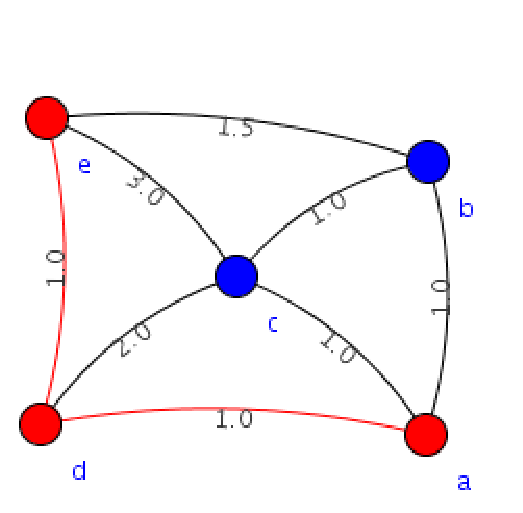
\includegraphics[scale=0.6]{./figs/grafoExemploTsETt.eps}}
%% \subfigure[�rvore $T_s$]{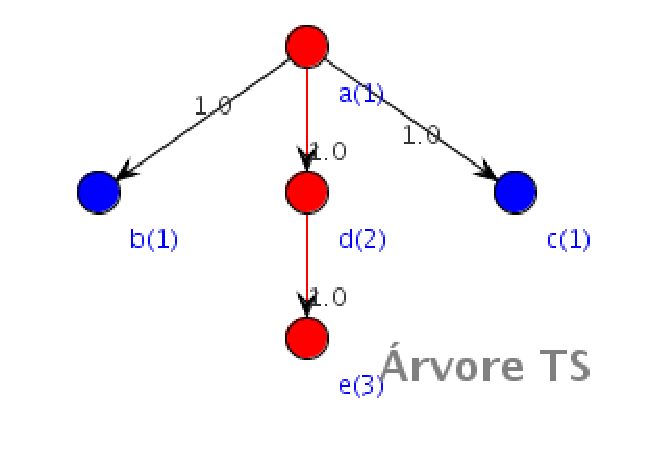
\includegraphics[scale=0.5]{./figs/exemploTs.eps}}
%% \subfigure[�rvore $T_t$]{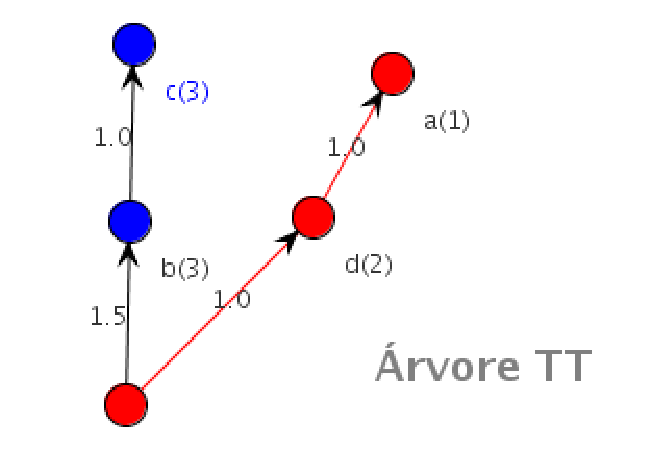
\includegraphics[scale=0.5]{./figs/exemploTt.eps}}
%% \caption{
%% Em (a) temos um grafo onde o menor caminho de $a$ a $e$ est� destacado.
%% Em (b) temos a �rvore de menores caminhos com raiz em $a$.
%% Em (c) temos a �rvore de menores caminhos com raiz em $e$. 
%% Nas �rvores o menor caminho de $a$ a $e$ encontra-se destacado.
%% }
%% \end{center}
%% \end{figure}
%% 
%% \newpage
%% \subsection*{Tipos de caminhos}
%% 
%% Seja $P=\seq{s=a_1,\ldots,a_{n}=t}$ um caminho de $s$ a $t$ no grafo sim�trico $(V,A,c)$, 
%% $T_s$ uma �rvore de menores caminhos com raiz em $s$,
%% $T_t$ uma �rvore de menores caminhos com raiz em $t$, $P \in T_s$, $P_r=\seq{t = a_n , \ldots , a_{1} = s }$, $P_r \in T_t$.
%% Um novo caminho de custo m�nimo diferente de $P$ constru�do atrav�s de $u \in V$ pode ser de um dos dois tipos definidos a seguir:
%% 
%% \begin{description}
%% \item[tipo I]: $s \underset{T_s}{\longrightarrow} u \underset{T_t}{\longrightarrow} t$. \mar{tipo I}
%% 
%% Onde $s\underset{T_s}{\longrightarrow}u$ representa o caminho de $s$ a $u$ na �rvore $T_s$ e 
%% $u\underset{T_t}{\longrightarrow}t$ representa o caminho $u$ a $t$ na �rvore 
%% $T_t$~\footnote{Pela simetria do grafo podemos afirmar que se existir o caminho de $t$ a $u$ ent�o o caminho de $u$ a $t$ tamb�m existir�.}.
%% O caminho $s\underset{T_s}{\longrightarrow}u$ se desvia do caminho $P=s\underset{T_s}{\longrightarrow}t$ em algum v�rtice de �ndice $\epsilon$
%% enquanto que o caminho $t\underset{T_t}{\longrightarrow}u$ se desvia de $P_r$ em algum v�rtice de �ndice $\zeta$.
%% 
%% Para montar um caminho deste tipo basta concatenar $s\underset{T_s}{\longrightarrow}u$ e $u\underset{T_t}{\longrightarrow}t$.
%% 
%% Observe que os caminhos $s \underset{T_s}{\longrightarrow} u$ e $u\underset{T_s}{\longrightarrow}t$ possuem apenas o v�rtice $u$ em comum.
%% \item[tipo II]: $s \underset{T_s}{\longrightarrow} u \underset{\in A}{\rightarrow} v \underset{T_t}{\longrightarrow} t$. \mar{tipo II}
%% 
%% O caminho de $s$ a $u$ est� em $T_s$ enquanto o caminho de $v$ a $t$ est� em $T_t$.
%% O arco $(u,v)$ n�o est� em $T_s$ nem em $T_t$, mas a aresta $(u,v)$ pertence ao grafo.
%% O caminho $s \underset{T_s}{\longrightarrow} u$ se desvia de $P$ em algum v�rtice de �ndice $\epsilon$ enquanto
%% que $t \underset{T_t}{\longrightarrow} v$ se desvia de $P_r$ num v�rtice de �ndice $\zeta$.
%% 
%% Para montar um caminho deste tipo basta concatenar $s\underset{T_s}{\longrightarrow}u$  ao v�rtice $v$ e depois ao caminho
%%  $v\underset{T_t}{\longrightarrow}t$.
%% 
%% Observe que os caminhos $s \underset{T_s}{\longrightarrow} u$ e $v\underset{T_t}{\longrightarrow}t$ n�o possuem v�rtices comuns.
%% \end{description}
%% 
%% Um desvio de um caminho $s \underset{T_s}{\longrightarrow} u$ � definido como o v�rtice a partir do qual ele
%% se torna diferente de $s \underset{T_s}{\longrightarrow} t$. 
%% Para cada desvio em $T_s$ definimos $\epsilon(desvio)$
%% como o n�mero de v�rtices do caminho $s \underset{T_s}{\longrightarrow} desvio$.
%% 
%% Um desvio de um caminho $t \underset{T_t}{\longrightarrow} u$ � definido como o v�rtice em que o caminho
%% se tornou diferente de $t \underset{T_t}{\longrightarrow} s$. 
%% Para cada desvio em $T_t$ definimos $\zeta(desvio)$
%% como o n�mero de v�rtices do caminho $t \underset{T_t}{\longrightarrow} desvio$.
%% 
%% Em ambos os casos, o desvio entre dois caminhos iguais � definido como o �ltimo v�rtice dos caminhos.
%% 
%% 
%% Para cada v�rtice $u$ podemos determinar que tipos de caminhos podem ser gerados a partir dele da seguinte maneira:
%% \begin{description}
%% \item[$\epsilon(u)<\zeta(u)$]:
%% O novo caminho ser� do tipo I.
%% \item[$\epsilon(u)=\zeta(u)$]: 
%% Se $u \in P$ ent�o isso sempre ocorre pela pr�pria defini��o.
%% No entanto, podem existir v�rtices n�o pertencentes a $P$ tal que isto tamb�m ocorra.
%% 
%% Neste caso, se tent�ssemos gerar um caminho do tipo I este conteria 
%% v�rtices repetidos, sendo assim um passeio e n�o um caminho, ou seria o pr�prio $P$. 
%% 
%% 
%% Vamos tratar de dois casos para mostrar que n�o � poss�vel montar um caminho do tipo I, diferente de $P$,
%%  a partir de $u$, quando $\epsilon(u)=\zeta(u)$:
%% \begin{description}
%% \item[$u \in P$]: 
%% Seja $u \in P=\seq{s=v_1,\ldots,u,\ldots,v_n=t}$, $s\underset{T_s}{\longrightarrow}u$ o caminho de $s$ a $u$ em $T_s$,
%% $P_r\seq{t=v_n,\ldots,u,\ldots,v_1=s}$ o reverso de $P$ em $T_t$ e $t\underset{T_t}{\longrightarrow}u$ o caminho de $t$ a $u$ em $T_t$.
%% Se concatenarmos os caminhos $s\underset{T_s}{\longrightarrow}u$ e $u\underset{T_t}{\longrightarrow}t$ teremos o caminho:
%% $\seq{s=v_1,\ldots,u,\ldots,v_n=t}=P$.
%% \item[$u \notin P$]:
%% Seja $u \notin P$ e escolha em $P$ o v�rtice $c$ tal que $\epsilon(c)=\epsilon(u)$, ou seja, escolha o v�rtice de desvio.
%% Vamos montar agora o caminho do tipo I: $s\underset{T_s}{\longrightarrow}u\underset{T_t}{\longrightarrow}t$.
%% Como $u$ se desvia de $P$ em $c$, temos $s\underset{T_s}{\longrightarrow}u=s\underset{T_s}{\longrightarrow}c\underset{T_s}{\longrightarrow}u$.
%% Como $\epsilon(c)=\zeta(c)$, pois $c \in P$, $\epsilon(u)=\zeta(u)$ e $\epsilon(c)=\epsilon(u)$, 
%% podemos afirmar que $c$ se desvia do reverso de $P$ no v�rtice $c$ logo, o caminho $u\underset{T_t}{\longrightarrow}t$ � igual
%% ao $u\underset{T_t}{\longrightarrow}c\underset{T_t}{\longrightarrow}t$.
%% Sendo assim, montar�amos o passeio: 
%% $s\underset{T_s}{\longrightarrow}c\underset{T_s}{\longrightarrow}u\underset{T_t}{\longrightarrow}c\underset{T_t}{\longrightarrow}t$, onde
%% observamos a repeti��o do v�rtice $c$, n�o sendo, portanto, um caminho.
%% \end{description}
%% 
%% 
%% 
%% Como vimos, podemos apenas gerar caminhos do tipo II, atrav�s de arcos $(u,v)\notin T_s \cup T_t$ contanto que 
%% $\epsilon(u)<\zeta(v)$. Se  $\epsilon(u) \geq \zeta(v)$, novamente gerar�amos passeios e n�o caminhos.
%% Usaremos um argumento parecido ao anteriormente apresentado.
%% Se $u \notin P$ tomaremos o v�rtice de desvio, ou seja, $c$ onde $\epsilon(u)=\epsilon(c)=\zeta(c)$,
%% se $u \in P$ tomaremos $c=u$.
%% Supondo que $\epsilon(u) \geq \zeta(v)$, como $\epsilon(u)=\epsilon(c)$, 
%% podemos escrever $\epsilon(c) \geq \zeta(v)$ ou $\zeta(c) \geq \zeta(v)$.
%% Tomemos agora o v�rtice de desvio de $v$, o qual chamaremos de $d$, tal que $\zeta(v)=\zeta(d)=\epsilon(d)$.
%% Montaremos agora o caminho do tipo II: $s\underset{T_s}{\longrightarrow}u \rightarrow v \underset{T_t}{\longrightarrow}t=
%% s\underset{T_s}{\longrightarrow}c\underset{T_s}{\longrightarrow}u \rightarrow v \underset{T_t}{\longrightarrow}d\underset{T_t}{\longrightarrow}t$.
%% Como $\zeta(c) \geq \zeta(v)$ e $\zeta(v)=\zeta(d)$ temos que $\zeta(c) \geq \zeta(d)$, assim, podemos reescrever o caminho
%% anterior como: $s\underset{T_s}{\longrightarrow}c\underset{T_s}{\longrightarrow}u \rightarrow v \underset{T_t}{\longrightarrow}c\underset{T_t}{\longrightarrow}d\underset{T_t}{\longrightarrow}t$,
%% onde fica clara a repeti��o do v�rtice $c$, caraterizando um passeio e n�o um caminho.
%% 
%% %Seja $u \notin P$ e escolha em $P$ o v�rtice $c$ tal que $\epsilon(c)=\epsilon(u)$, ou seja, escolha o v�rtice de desvio.
%% %Basta notar que $\epsilon(u)>\zeta(v)$ significa que o caminho $s \underset{T_s}{\longrightarrow} u$ se desviou de
%% %s \underset{T_s}{\longrightarrow} t$ no v�rtice $u_{\epsilon}$ e o caminho $v \underset{T_t}{\longrightarrow} t$
%% %se desviou de $P_r$ no v�rtice $u_{\zeta}$. 
%% %Ent�o, $s \underset{T_s}{\longrightarrow} u=\seq{u_1,\ldots,u_{\epsilon}}$ e
%% %v \underset{T_t}{\longrightarrow} t=\seq{u_{\zeta},\ldots,u_n}$. 
%% %Sendo $\epsilon(u)>\zeta(v)$, fica claro que a concatena��o dos caminhos
%% %gerar� um passeio com v�rtices repetidos.
%% \item[$\epsilon(u)>\zeta(u)$]
%% S� podemos gerar passeios neste caso.
%% \end{description}
%% 
%% 
%% 
%% %\subsection*{Tipos de caminhos}
%% %Dadas duas �rvores, $T_s$ e $T_t$ e um natural $\alpha$ o algoritmo de KIM pode gerar caminhos de dois tipos distintos: 
%% %%\item[tipo I]: $s \underset{T_s}{\longrightarrow} u \underset{T_t}{\longrightarrow} t$ e  $\epsilon(u) < \alpha$. \mar{tipo I}.
%% %Onde $s\underset{T_s}{\longrightarrow}u$ representa o caminho de $s$ a $u$ na �rvore $T_s$ e 
%% %$u\underset{T_t}{\longrightarrow}t$ representa o caminho $u$ a $t$ na �rvore $T_t$.
%% %% Pela simetria do grafo podemos afirmar que se existir o caminho de $t$ a $u$ ent�o o caminho de $u$ a $t$ tamb�m existir�.
%% 
%% %% \item[tipo II]: $s \underset{T_s}{\longrightarrow} u \underset{\in A}{\rightarrow} v \underset{T_t}{\longrightarrow} t$ e  $\epsilon(u) < \alpha$. \mar{tipo II}
%% %% O caminho de $s$ a $u$ est� em $T_s$ enquanto o caminho de $v$ a $t$ est� em $T_t$.
%% %% A aresta $(u,v)$ est� em $A$ mas o arco $(u,v)$ n�o est� em $T_s$.
%% %% \end{description}
%% 
%% 
%% %% 
%% %% Utilizando a figura~\ref{fig:rotulacao} e $\alpha=2$ ter�amos, por exemplo, o seguinte caminho do tipo I: $\seq{a,b,e}$.
%% %% Neste exemplo, usamos $s=a, t=e, u=b$ e $\epsilon(b)=1<\alpha$ e obtivemos o caminho de $s$ a $b$ em $T_s$ e o concatenamos
%% %% ao caminho de $b$ a $t$ em $T_t$, ou seja, concatenamos os caminhos $\seq{a,b}$ e $\seq{b,e}$.
%% 
%% 
%% 
%% %% 
%% %% Utilizando a mesma figura, o mesmo $\alpha$ e $s=a,t=e,u=c,\epsilon(c)<\alpha$ obtemos o caminho do tipo II: $\seq{a,c,d,e}$.
%% %% Neste caso, estamos concatenando o caminho $\seq{a,c} \in T_s$ ao arco $(c,d) \notin T_s \cup T_t$ ao 
%% %% caminho $\seq{d,e} \in T_t$. 
%% 
%% A rotina \FSP{} � utilizada para a gera��o de desvios de custo m�nimo, sendo portanto, subrotina
%% nas gera��es de caminhos nas parti��es: $P_a,P_b$ e $P_c$.
%% A seguir apresentamos com mais detalhes cada uma dessas parti��es.

\section{Parti��es}
\label{sec:particoes}
Nesta se��o trataremos das parti��es definidas em cada itera��o do algoritmo \KIM.
Relembrando o funcionamento do algoritmo, 
inicialmente calculamos o caminho $P_1$, menor caminho entre $s$ e $t$, 
utilizando um algoritmo \PCM.
Em seguida, utilizando a rotina \FSP{}, obtemos um desvio m�nimo de $P_1$, chamado de $P_2$. 
A partir de $P_2$ e seu pai, $P_1$, definimos tr�s parti��es do conjunto de caminhos de $s$ a $t$:
\begin{description}
\item[$P_a$]: \mar{$P_a$} caminhos que desviam de $P_2$ em algum momento depois que $P_2$ se desviou de $P_1$.
\item[$P_b$]: \mar{$P_b$} caminhos que desviam de $P_1$ depois do v�rtice comum a $P_1$ e $P_2$.
\item[$P_c$]: \mar{$P_c$} caminhos que desviam de $P_1$ antes do v�rtice comum a $P_1$ e $P_2$.
\end{description}
Cada uma das parti��es � representada por um caminho de menor custo pertencente a ela.
A partir de $P_1$ e $P_2$ s�o gerados, no m�ximo, tr�s novos caminhos,
 os representantes das parti��es descritas acima, 
os quais ser�o candidatos para $P_3$.
%% A partir dos caminhos $P_1$ e $P_2$ s�o gerados, no m�ximo, tr�s novos caminhos, os quais ser�o candidatos para 
%% $P_3$, s�o eles:
%% \begin{description}
%% \item[$P_a$]: \mar{$P_a$}menor caminho que se desvia de $P_2$ em algum momento depois que $P_2$ se desviou de $P_1$.
%% \item[$P_b$]: \mar{$P_b$}menor caminho que se desvia de $P_1$ depois do v�rtice comum a $P_1$ e $P_2$.
%% \item[$P_c$]: \mar{$P_c$}menor caminho que se desvia de $P_1$ antes do v�rtice comum a $P_1$ e $P_2$.
%% \end{description}

Na figura a seguir vemos a disposi��o esquem�tica das parti��es $P_a,P_b$ e $P_c$.
\begin{figure}[htbp]
\centering
  \begin{tikzpicture}[scale=0.70]
    \tikzstyle{node}=%
    [%
      inner sep=0pt,%
      outer sep=0pt,%
      ball color=red,%
      circle%
    ]
        \node[node,minimum size=8pt,label=left:{s}] at (0,3) (S)  {};
        \node[node] at (1,3) (A)  {};
        \node[node] at (2,3) (B)  {};
        \node[node] at (3,3) (C)  {};
        \node[node] at (4,1) (D)  {};
        \node[node,minimum size=8pt,label=right:{t}] at (11,3) (T) {};
       
        \node[color=red] at (6,3.2) (P1) {P1};

        \path [-,thick,red]  
                  (S) edge[] (T)
                  (S) edge (A)
                  (A) edge (B)
                  (B) edge (C);

        \path [-,thick,blue]  
                  (B) edge[bend right] (D)
                  (D) edge[bend right] (T);
         \node[color=blue] at (6,1) (P2) {P2};



        \path [-,thick,black,dashed]  
                  (A.north) edge[in=90] (T.north);
                 \node[color=black] at (6,5.8) (Pc) {Pc};
        \path [-,thick,black,dashed]  
                  (C.north) edge[bend left] (T.north);
                 \node[color=black] at (6,4.5) (Pb) {Pb};
        \path [-,thick,black,dashed]  
                  (D) edge[in=-90,out=-90] (T);
                 \node[color=black] at (6,0) (Pa) {Pa};

        \end{tikzpicture}
\caption[Disposi��o dos representantes das parti��es $P_a$, $P_b$ e $P_c$]
{Disposi��o esquem�ticas dos representantes das parti��es $P_a$, $P_b$ e $P_c$}
\end{figure}

� poss�vel observar que s� existem estas tr�s possibilidades para o caminho $P_3$. 
Os representantes das parti��es: $P_a$, $P_b$ e $P_c$, s�o ent�o colocados na lista de caminhos candidatos e, 
no in�cio da pr�xima itera��o,
um caminho de menor custo � retirado da lista, tornando-se o $P_3$.
A partir dos caminhos $P_3$ e seu caminho pai, faremos o mesmo processo, ou seja,
geraremos tr�s caminhos candidatos em cada uma das parti��es:$P_a$, $P_b$, $P_c$, definidas por $P_3$ e seu pai.
O pai de cada caminho � definido da seguinte maneira:
\begin{itemize}
\item O pai de $P_a$ � o $P_2$;
\item O pai de $P_b$ � o $P_1$;
\item O pai de $P_c$ � o $P_1$;
\item O pai de $P_2$ � o $P_1$.
\end{itemize}
Uma defini��o melhor de caminho pai seria:
Dada uma seq��ncia ordenada de caminhos $\seq{P_1,P_2, \ldots P_k}$, onde $\forall j\leq i, c(P_j)\leq c(P_i) $, 
diremos que $P_j$ � pai de $P_i$, quando
$i=min\{x| 1 < x < j, \mbox{tal que $P_j$ e $P_i$ compartilham o maior prefixo comum\}}$. 

Seja, por exemplo, \\
$P=\seq{\seq{a,b,e},\seq{a,c,e},\seq{a,d,e},\seq{a,b,c,e}}$. \\
O pai do caminho $\seq{a,d,e}$ � o $\seq{a,b,e}$. 
Embora o caminho $\seq{a,c,e}$ compartilhe o mesmo prefixo que $\seq{a,b,e}$, ele possui um �ndice maior e, 
na defini��o dizemos que o $i$ deve ser o menor �ndice tal que tenha o maior prefixo.

%% \newpage
%% \begin{figure}[hbp]
%% \begin{center}
%%     \psfrag{P1}{{$P_1$}}
%%     \psfrag{P2}{{$P_2$}}
%%     \psfrag{Pa}{{$P_a$}}
%%     \psfrag{Pb}{{$P_b$}}
%%     \psfrag{Pc}{{$P_c$}}
%% 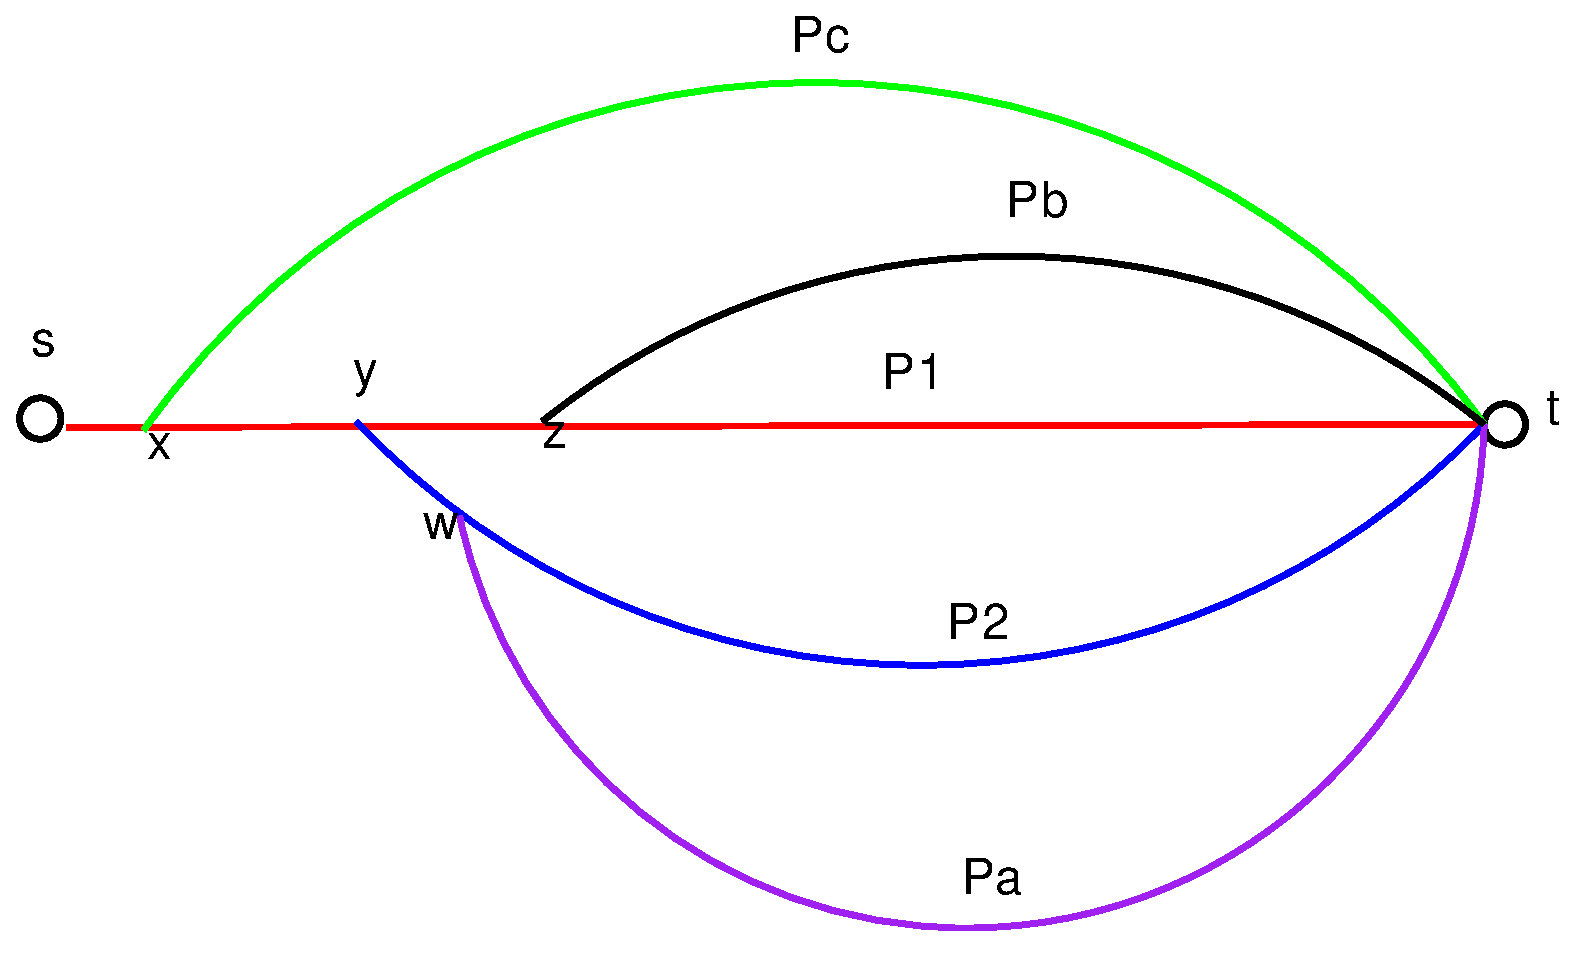
\includegraphics[scale=0.3]{./figs/kimCaminhos.eps}
%% \caption{A partir do menor caminho, $P_1$, calculamos o segundo menor caminho, $P_2$. 
%% $P_1$ e $P_2$ servem como base para a defini��o das parti��es: $P_a,P_b$ e $P_c$.
%% }
%% \label{fig:caminhosDerivados}
%% \end{center}
%% \end{figure}

%% Seja $(V,A,c)$ um grafo sim�trico com custos nas arestas, $s$ e $t$dois v�rtices distintos de $V$,
%% $\seq{P_1,P_2,\ldots,P_k}$ uma lista de menores caminhos de $s$ a $t$ em $(V,A,c)$ tal que $c(P_1)\leq c(P_2)\leq \ldots,c(P_k)$,
%% cada par de caminhos $P_i,P_j$, onde $P_i$ � pai de $P_j$, determina tr�s parti��es dos caminhos de $s$ a $t$, chamadas de
%% $P_{a_j},P_{b_j},$ e $P_{c_j}$.
%% 
%% Em cada itera��o do algoritmo, o conjunto $\Pcal_{st}$ pode ser reparticonado, rece

Agora que vimos como s�o as parti��es definidas para os caminhos $P_1$ e $P_2$, mostraremos
sua defini��o em fun��o de um $i-$�simo caminho qualquer.

Antes de prosseguirmos vale lembrar alguns pontos sobre �rvore dos prefixos~(se��o~\ref{sec:prefixos}).
Dado um grafo e uma cole��o de caminhos com ponta inicial $s$, existe uma �rvore dos prefixos 
desses caminhos representada por $(N,E,f)$, onde $N$ � ao conjunto de n�s, $E$ � o conjunto de arcos
e $f$ � uma fun��o r�tulo que relaciona n�s � caminhos na �rvore a v�rtices e caminhos no grafo.

Seja $u$ um n� em $(N,E,f)$, ent�o:
\begin{itemize}
\item $R_u$ � o caminho, com origem na raiz, com ponta final em $u$;
\item $A_u$ � conjunto de arcos com ponta inicial em $u$;
\item $f(R_u)$ mapeia o caminho $R_u$ na �rvore ao caminho correspondente de $a$ a $f(u)$ no grafo.
\end{itemize}

\newpage
\subsection*{Parti��o $P_a$}

Seja $(V,A,c)$ um grafo sim�trico com um fun��o custo definida em suas arestas,
$\Qcal=\seq{P_1,\ldots,P_i}$, onde $i \geq 2$, o conjunto dos $i-$menores caminhos de $s$ a $t$, 
$P_j$ o caminho pai de $P_i$, $\delta$ o v�rtice de desvio entre $P_j$ e $P_{i}$, 
$\beta$ o �ndice de $\delta$ em $P_i=\seq{s=u_1,\ldots,u_n=t}$,
$(N,E,f)$ a �rvore dos prefixos de $\Qcal$ e
$f(R_p)=\seq{s=u_1,\ldots,u_{\beta}}$.
%$f(R_q)=\seq{s=u_1,\ldots,u_{\beta+1}}$.

A parti��o $P_a$, definida por $P_j$ e $P_i$, corresponde ao conjunto de caminhos de $s$ a $t$, com prefixo $f(R_q)$ e que sejam 
diferentes de $P_i$.
%n�o possuem o o prefixo arcos em $A_q$.

Para gerar caminhos m�nimos em $P_a$, removemos do grafo os v�rtices do prefixo $f(R_p)$ juntamente 
com suas arestas, ou seja, removemos os v�rtices $\seq{u_1,\ldots,u_{\beta}=\delta}$ e as arestas com pontas nestes v�rtices.
Logo ap�s, geramos um desvio m�nimo de $u_{\beta+1}$ a $u_n=t$, executando para isso a rotina \FSP{}
no grafo alterado, tomando $u_{\beta+1}$ como origem, $u_n=t$ como destino, 
$P=\seq{u_{\beta+1},\ldots,u_n=t}$ e $\alpha=|P|$, a qual nos retorna um caminho de custo m�nimo 
de $u_{\beta+1}$ a $t$ diferente de $P$.
Concatenando o caminho encontrado ao prefixo $f(R_p)$ obtemos um caminho de custo m�nimo na parti��o $P_a$.

Todo caminho na parti��o $P_a$, definida por $P_j$ e $P_i$, � filho de $P_i$.

A seguir, o algoritmo que sintetiza o que foi descrito:

\begin{algoritmo}

\textbf{Algoritmo} \Pa{} $(V,A,c,\Qcal,P)$ %\\[2mm]
\index{algoritmo!KIM@\Pa}\index{KIM@\Pa}
   
0\x $P$ definido por $\seq{u_1,\ldots u_n}$

1\x $(N,E,f) \larr$ �rvore dos prefixos de $\Qcal$

2\x $\beta \larr$ �ndice do v�rtice $\delta$

3\x $V^{'} \larr V - \seq{u_1,\ldots,u_{\beta}}$ 

4\x $A^{'} \larr A - \{uv| u \mbox{ ou } v \in \seq{u_1,\ldots,u_{\beta}}\}$
%5\x $P_a \larr f(R_p) \cup \FSP~(V^{'},A^{'},c,u_{\beta+1},t,\seq{u_{\beta+1},\ldots,t},|\seq{u_{\beta+1},\ldots,t}|)$

5\x \devolva{} $f(R_p) \cup \FSP~(V^{'},A^{'},c,u_{\beta+1},t,\seq{u_{\beta+1},\ldots,t},|\seq{u_{\beta+1},\ldots,t}|)$

\end{algoritmo}

As altera��es no grafo executadas nas linhas~3 e 4 consomem tempo $\Oh(m+n)$.
O custo da linha~5 � o mesmo da fun��o \FSP{}, consumo este, dominante na cria��o do caminho de menor custo na parti��o $P_a$.
Assim, o consumo de tempo da rotina \Pa{} � $\Theta(T(n,m))$.

Na figura a seguir, temos uma �rvore dos prefixos de $\Qcal$, onde apenas exibimos 
os caminhos $P_j$ e $P_i$, representados, respectivamente, 
pelos n�s $t_j$ e $t_i$.
Os r�tulos externos representam v�rtices no grafo, enquanto que os internos, n�s na �rvore dos prefixos.
As linhas tracejadas representam uma seq��ncia de n�s e arcos.
As linhas cont�nuas representam um n� ou arco espec�fico.

\begin{figure}[htbp]
\centering
\tikzstyle{node}=[circle,fill=black!25,minimum size=10pt,inner sep=0pt]
\tikzstyle{root} = [node, fill=red!24]
\tikzstyle{leaf} = [node, fill=red!24]
\tikzstyle{deviation} = [node, fill=blue!50]
\tikzstyle{onPath} = [node, dashed,fill=red!24]
\tikzstyle{edge} = [draw,thick,->]
\tikzstyle{unknown} = [dashed,thick,->]
\tikzstyle{novos} = [node, fill=red!50]
\tikzstyle{weight} = [font=\tiny]
\tikzstyle{selected edge} = [draw,thick,->,red!50]
%\tikzstyle{LabelStyle}=[fill=white,sloped]
\begin{tikzpicture}[scale=1]
% Set the overall layout of the tree
\tikzstyle{level 1}=[level distance=1.5cm, sibling distance=2.5cm]
\tikzstyle{level 2}=[level distance=1.5cm, sibling distance=2.5cm]
\node[root,label=right:{s}] (s1) {}
child {
				node[deviation,label=right:{$\delta$}] {$p$}
				child[->,solid] {
						node[node] {a}
						child[->,dashed]{
							node[leaf] {$t_j$}
						}
				}
				child[->,solid] {
					node[node] {$q$}
						child[grow=down,dashed]{
							node[leaf] {$t_{i}$} 
						}
				}
				edge from parent[dashed]
};


\node[root,label=right:{s},right of=s1,node distance=4cm] (s2) {}
child {
				node[deviation,label=right:{$\delta$}] {$p$}
				child[->,solid] {
						node[node] {a}
						child[->,dashed]{
							node[leaf] {$t_j$}
						}
				}
				child[->,solid] {
					node[node] {$q$}
						child[sibling distance=10mm,level distance=1cm,dashed,->,line width=2pt]{node[novos]{}}
						child[sibling distance=10mm,level distance=1cm,dashed,->]{
							child[dashed,line width=2pt]{node[novos]{}}
							child[line width=2pt]{node[novos]{}}
							child[level distance=1.5cm,grow=down]{
								node[leaf] {$t_{i}$} 
							}
							child[line width=2pt]{node[novos]{}}
							child[line width=2pt]{node[novos]{}}
						}
						child[sibling distance=10mm,level distance=1cm,dashed,->,line width=2pt]{node[novos]{}}
					}
				edge from parent[dashed]
};
\end{tikzpicture}
\caption{Esquema dos caminhos na parti��o $P_a$ definida por $P_j$ e $P_i$}
\end{figure}

O v�rtice de desvio entre $P_j$ e $P_i$ � o $\delta$.
Na figura � direita, vemos os caminhos da parti��o $P_a$, definida por $P_j$ e $P_i$, 
que correspondem aos caminhos que desviam de $P_i$ ap�s o n� $q$.


\subsection*{Parti��o $P_b$}

Seja $(V,A,c)$ um grafo sim�trico com um fun��o custo definida em suas arestas,
$\Qcal=\seq{P_1,\ldots,P_i}$, onde $i \geq 2$, o conjunto dos $i-$menores caminhos de $s$ a $t$, 
$P_j$ o caminho pai de $P_i$, $\delta$ o v�rtice de desvio entre $P_j$ e $P_{i}$, 
$\beta$ o �ndice de $\delta$ em $P_j=\seq{s=u_1,\ldots,u_n=t}$,
$(N,E,f)$ a �rvore dos prefixos de $\Qcal$,
$f(R_p)=\seq{s=u_1,\ldots,u_{\beta}}$ e 
$f(R_q)=\seq{u_1,\ldots,u_{\beta+1}}$.

A parti��o $P_b$, definida por $P_j$ e $P_i$, corresponde ao conjunto de caminhos com prefixo $f(R_p)$ que
n�o possuem arcos em $A_p - (p,q)$ e que desviam de $P_j$ antes do v�rtice $u_{\gamma}$.
Para o c�lculo de $\gamma$, escolha o caminho $P_l$ que compartilha com $P_j$ o menor prefixo $f(R_r)$ 
tal que $f(R_p) \subset f(R_r)$, e temos $u_{\gamma}=f(r)$.

%% Sejam $\Qcal=\seq{P_1,\ldots,P_{k-1}}$ o conjunto dos $k-1$, $k \geq 3$ caminhos de $s$ a $t$, 
%% $P_j=\seq{s=u_1,\ldots,u_n=t}$ o caminho pai de $P_{i}$,
%% $\delta$ o v�rtice de desvio entre $P_j$ e $P_{i}$, 
%% $\beta$ o �ndice de $\delta$ em $P_j$,
%% todo caminho da parti��o $P_b$ � filho de $P_j$.
%% 
%% Sejam $(N,E,f)$ uma �rvore de prefixos formada a partir de $\Qcal$,
%% $f(R_p)=\seq{u_1,\ldots,u_{\beta}}$,
%% $f(R_q)=\seq{u_1,\ldots,u_{\beta+1}}$,
%% a parti��o $P_b$ corresponde ao conjunto de caminhos com prefixo $f(R_p)$ que
%% n�o possuem arcos em $A_p - (p,q)$ e que se
%% desviam de $P_j$ antes do v�rtice $u_{\gamma}$.
%% Para o c�lculo de $\gamma$, escolha o caminho $P_l$ que compartilha com $P_j$ o menor prefixo $f(R_r)$ tal que $f(R_p) \subset f(R_r)$,
%% e temos $u_{\gamma}=f(r)$.

Para gerar caminhos nesta parti��o, removemos do grafo os v�rtices do prefixo $f(R_p)$, com exce��o de $f(p)$ juntamente 
com suas arestas, ou seja, removemos os v�rtices $\seq{u_1,\ldots,u_{\beta-1}}$ e as arestas com pontas nestes v�rtices.
Al�m disso, removemos as arestas $f(a)f(b), \forall (a,b) \in A_p$, com exce��o da aresta $u_{\beta}u_{\beta+1}$.
 
Logo ap�s, executamos a rotina \FSP{} com o novo grafo, $\delta$ como origem, $u_n=t$ como destino, 
$P=\seq{\delta,\ldots,u_n=t}$ e $\alpha=|\seq{\delta,\ldots,u_{\gamma}}|$, 
obtendo ent�o um caminho de custo m�nimo de $\delta$ a $t$ diferente de $P$ e que desvia deste antes do v�rtice $u_{\gamma}$.
Concatenando o prefixo $f(R_p)$ ao caminho encontrado obtemos o caminho de menor custo na parti��o $P_b$.

Todo caminho na parti��o $P_b$ definida por $P_j$ e $P_i$ � filho de $P_j.$

A seguir o algoritmo que sintetiza o procedimento descrito:


\begin{algoritmo}

\textbf{Algoritmo} \Pb{} $(V,A,c,\Qcal,P)$ %\\[2mm]
\index{algoritmo!KIM@\Pb}\index{KIM@\Pb}
   
0\x $P_j \larr$ pai de $P$ 

1\x $P_j$ definido por $\seq{u_1,\ldots u_n}.$

2\x $(N,E,f) \larr$ �rvore dos prefixos de $\Qcal$

3\x $\delta \larr$ v�rtice de desvio de $P$ e $P_j$

4\x $\beta \larr$ �ndice do v�rtice $\delta$

5\x $V^{'} \larr V - \seq{u_1,\ldots,u_{\beta - 1}}$ 

6\x $A^{'} \larr A - \{uv|u \mbox{ ou } v \in \seq{u_1,\ldots,u_{\beta-1}}\}$ 

7\x $A^{'} \larr A^{'} - f(a)f(b), \forall (a,b) \in A_p$

8\x $A^{'} \larr A^{'} \cup u_{\beta}u_{\beta+1}  \in P_j$

9\x $u_{\gamma}=f(r)$ sendo $f(R_r), com f(R_p) \subset f(R_r)$, o menor prefixo 

\xx compartilhado por $P_j$ e algum caminho de $\Qcal$

10\x \devolva{} $f(R_p) \cup \FSP~(V^{'},A^{'},c,\delta,t,\seq{u_{\beta},\ldots,u_n=t},|\seq{u_{\beta},\ldots,u_{\gamma}}|)$

\end{algoritmo}

Assim como aconteceu no c�lculo do consumo de tempo do caminho de custo m�nimo na parti��o $P_a$, o
consumo do algoritmo \Pb{} � dominado pela chamada � fun��o \FSP{}, sendo portanto
$\Theta(T(n,m))$.

Na figura a seguir temos em (a) uma �rvore dos prefixos dos caminhos em $\Qcal$, 
onde exibimos os caminhos $P_i$ e $P_j$ representados, respectivamente,
pelos caminhos da raiz �s folhas $t_i$ e $t_j$.
As folhas em \textcolor{green!50}{verde} representam caminhos filhos de $P_j$, que desviam deste ap�s o n� $\delta$.
Em (b) vemos como � feita a escolha do n� $r$ a partir dos filhos de $P_j$.
Em (c), exibimos, usando folhas \textcolor{red!70}{vermelhas}, os caminhos da parti��o $P_b$ definida pelos caminhos $P_i$ e $P_j$, correspondentes
aos caminhos com prefixo $f(R_p)$ e que desviam de $P_j$ antes do v�rtice $u_{\gamma}$.
\begin{figure}[htbp]
\centering
\tikzstyle{node}=[circle,fill=black!25,minimum size=10pt,inner sep=0pt]
\tikzstyle{root} = [node, fill=red!24]
\tikzstyle{leaf} = [node, fill=red!24]
\tikzstyle{novos} = [node, fill=red!70]
\tikzstyle{deviation} = [node, fill=blue!50]
\tikzstyle{onPath} = [node, dashed,fill=red!24]
\tikzstyle{edge} = [draw,thick,->]
\tikzstyle{unknown} = [dashed,thick,->]
\tikzstyle{filhos} = [node,fill=green!50]
\tikzstyle{weight} = [font=\tiny]
\tikzstyle{selected edge} = [draw,thick,->,red!50]
%\tikzstyle{LabelStyle}=[fill=white,sloped]
\begin{tikzpicture}[scale=1]
% Set the overall layout of the tree
\tikzstyle{level 1}=[level distance=1.5cm, sibling distance=2.5cm]
\tikzstyle{level 2}=[level distance=1cm, sibling distance=2cm]
\node[root,label=right:{s}] (s1) {}
child {
				node[deviation,label=right:{$\delta$}] {$p$}
				child[->,dashed]{node[filhos]{}}
				child[->,solid]{
				node[node]{$q$}
				child[->,dashed] {
						child[->,dashed]{node[filhos]{}}
						child[-,dashed,grow=down]{
							child[-,dashed]{
													node {$\ldots$}
													edge from parent[draw=none]
							}
							child[->,dashed,grow=down,label distance=8mm]{
													child[->,dashed]{
																			node[filhos]{}
													}
													child[->,dashed,grow=down]{
																			node[leaf,label=below:{(a)}] {$t_j$}
													}
							}
						}
				}
				}
				child[->,solid] {
					node[node] {}
						child[grow=down,dashed]{
							node[leaf] {$t_{i}$} 
						}
				}
				edge from parent[dashed]
};
\node[root,label=right:{s},right of=s1,node distance=5cm] (s2) {}
child {
				node[deviation,label=right:{$\delta$}] {$p$}
				child[->,dashed]{node[filhos]{}}
				child[->,dashed] {
						node[deviation,label=right:{$u_{\gamma}$}] {$r$}
						child[->,dashed]{node[filhos]{$t_l$}}
						child[-,dashed,grow=down]{
							child[-,dashed]{
													node {$\ldots$}
													edge from parent[draw=none]
							}
							child[->,dashed,grow=down,label distance=18mm]{
													child[->,dashed]{
																			node[filhos]{}
													}
													child[->,dashed,grow=down]{
																			node[leaf,label=below:{(b)}] {$t_j$}
													}
							}
						}
				}
				child[->,solid] {
					node[node] {}
						child[grow=down,dashed]{
							node[leaf] {$t_{i}$} 
						}
				}
				edge from parent[dashed]
};

\node[root,label=right:{s},right of=s2,node distance=5cm] (s3) {}
child[sibling distance=15mm] {
				node[deviation,label=right:{$\delta$}] {$p$}
				child[->,dashed,line width=2pt,sibling distance=15mm]{node[novos]{}}
				child[->,dashed,sibling distance=15mm]{node[filhos]{}}
				child[grow=down,sibling distance=15mm]{
					child[->,dashed,line width=2pt]{node[novos]{}}
					child[grow=down,level distance=5mm]{
						child[level distance=10mm,grow=south east,->,dashed,line width=2pt]{node[novos]{}}
						child[level distance=15mm,->,dashed,grow=down] {
								node[deviation,label=right:{$u_{\gamma}$}] {$r$}
								child[level distance=10mm,->,dashed]{node[leaf]{$t_l$}}
								child[level distance=10mm,->,dashed,grow=down,label distance=18mm]{
										node[leaf,label=below:{(c)}] {$t_j$} 
								}
						}
					}
				}
				child[->,solid,sibling distance=15mm] {
					node[node] {}
						child[grow=down,dashed]{
							node[leaf] {$t_i$} 
						}
				}
				edge from parent[dashed]
};
\end{tikzpicture}
\caption{Esquema dos caminhos na parti��o $P_b$ definida por $P_j$ e $P_i$}
\end{figure}


\subsection*{Parti��o $P_c$}

Seja $(V,A,c)$ um grafo sim�trico com um fun��o custo definida em suas arestas,
$\Qcal=\seq{P_1,\ldots,P_i}$, onde $i \geq 2$, o conjunto dos $i-$menores caminhos de $s$ a $t$, 
$P_j$ o caminho pai de $P_i$, $\delta$ o v�rtice de desvio entre $P_j$ e $P_{i}$, 
$\beta$ o �ndice de $\delta$ em $P_j=\seq{s=u_1,\ldots,u_n=t}$,
$(N,E,f)$ a �rvore dos prefixos de $\Qcal$,
$f(R_p)=\seq{s=u_1,\ldots,u_{\beta}}$,
$f(R_q)$ o maior prefixo de um caminho em $\Qcal$ tal que $f(R_q) \subset f(R_p)$ e
$u_{\lambda}=f(q)$.

A parti��o $P_c$, definida por $P_j$ e $P_i$, corresponde ao conjunto de caminhos com prefixo $f(R_q)$ que
n�o possuem arcos em $A_p$ e que desviam de $P_j$ antes do v�rtice $f(p)$.
%$f(R_q)=\seq{u_1,\ldots,u_{\beta+1}}$.

%% Sejam $\Qcal=\seq{P_1,\ldots,P_{k-1}}$ o conjunto dos $k-1$, $k \geq 3$, caminhos de $s$ a $t$, 
%% $P_j=\seq{s=u_1,\ldots,u_n=t}$ o caminho pai de $P_{k-1}$,
%% $\delta$ o v�rtice de desvio entre $P_j$ e $P_{k-1}$, 
%% $\beta$ o �ndice de $\delta$ em $P_j$,
%% todo caminho da parti��o $P_c$ � filho de $P_j$.

%% Sejam $(N,E,f)$ uma �rvore de prefixos formada a partir de $\Qcal$,
%% $f(R_p)=\seq{u_1,\ldots,u_{\beta}}$,
%% $f(R_q)$ o maior prefixo de um caminho em $\Qcal$ tal que $f(R_q) \subset f(R_p)$,
%% a parti��o $P_c$ corresponde ao conjunto de caminhos com prefixo $f(R_q)$ que
%% n�o possuem arcos em $A_p$ e que se
%% desviam de $P_j$ antes do v�rtice $f(p)$.


Para gerar caminhos nesta parti��o, removemos do grafo os v�rtices do prefixo $f(R_q)$, com exce��o de $f(q)$, juntamente 
com suas arestas, ou seja, removemos os v�rtices $\seq{u_1,\ldots,u_{\lambda-1}}$ e as arestas com pontas nestes v�rtices.
Al�m disso, removemos as arestas $f(a)f(b)\mbox{ }\forall (a,b) \in A_q$.
 
Executamos ent�o a rotina \FSP{} com o novo grafo, $u_{\lambda}$ como origem, $t$ como destino, 
$P=\seq{u_{\lambda},\ldots,t}$ e $\alpha=|\seq{u_{\lambda},\ldots,u_{\beta}}|$, 
obtendo ent�o um caminho de custo m�nimo de $u_{\lambda}$ a $t$ diferente de $P$ e que desvia deste antes do v�rtice $u_{\beta}$.
Concatenando o prefixo $f(R_q)$ ao caminho encontrado obtemos o caminho de menor custo na parti��o $P_c$.

Todo caminho na parti��o $P_c$ definida por $P_j$ e $P_i$ � filho de $P_j.$

A seguir o algoritmo que sintetiza o procedimento descrito:

\begin{algoritmo}

\textbf{Algoritmo} \Pc{} $(V,A,c,\Qcal,P)$ %\\[2mm]
\index{algoritmo!KIM@\Pc}\index{KIM@\Pc}
   
0\x $P_j \larr$ pai de $P$ 

1\x $P_j$ definido por $\seq{u_1,\ldots u_n}.$

2\x $(N,E,f) \larr$ �rvore dos prefixos de $\Qcal$

3\x $\delta \larr$ v�rtice de desvio de $P$ e $P_j$

4\x $\beta \larr$ �ndice do v�rtice $\delta$

5\x $f(R_p) \larr \seq{u_1,\ldots,u_{\beta}}$

6\x $u_{\lambda}=f(q)$ onde $f(R_q)$ � o maior prefixo 

\xx de um caminho em $\Qcal$ tal que $f(R_q) \subset f(R_p)$

7\x $V^{'} \larr V - \seq{u_1,\ldots,u_{\lambda - 1}}$ 

8\x $A^{'} \larr A - \{uv|u \mbox{ ou } v \in \seq{u_1,\ldots,u_{\lambda-1}}\}$ 

9\x $A^{'} \larr A^{'} - f(a)f(b), \forall (a,b) \in A_q$

10\x \devolva{} $f(R_q) \cup \FSP~(V^{'},A^{'},c,u_{\lambda},t,\seq{u_{\lambda},\ldots,u_n=t},|\seq{u_{\lambda},\ldots,u_{\beta}}|)$

\end{algoritmo}

Assim como aconteceu no c�lculo do consumo de tempo do caminho de custo m�nimo na parti��o $P_b$, o
consumo do algoritmo \Pc{} � dominado pela chamada � fun��o \FSP{}, sendo portanto
$\Theta(T(n,m))$.

Na figura a seguir exibimos uma �rvore dos prefixo resumida dos caminhos em $\Qcal$, onde destacamos os caminhos $P_j$
e $P_i$ definidos pelos caminhos com in�cio na raiz e t�rmino, respectivamente, nas folhas $t_j$ e $t_i$.
\begin{figure}[htbp]
\centering
\tikzstyle{node}=[circle,fill=black!25,minimum size=10pt,inner sep=0pt]
\tikzstyle{root} = [node, fill=red!24]
\tikzstyle{leaf} = [node, fill=red!24]
\tikzstyle{novos} = [node, fill=red!70]
\tikzstyle{deviation} = [node, fill=blue!50]
\tikzstyle{onPath} = [node, dashed,fill=red!24]
\tikzstyle{edge} = [draw,thick,->]
\tikzstyle{unknown} = [dashed,thick,->]
\tikzstyle{filhos} = [node,fill=green!50]
\tikzstyle{weight} = [font=\tiny]
\tikzstyle{selected edge} = [draw,thick,->,red!50]
%\tikzstyle{LabelStyle}=[fill=white,sloped]
\begin{tikzpicture}[scale=1]
% Set the overall layout of the tree
\tikzstyle{level 1}=[level distance=5mm, sibling distance=2cm]
\tikzstyle{level 2}=[level distance=5mm, sibling distance=2cm]
\node[root,label=right:{s}] (s1) {}
child {
	child[->,dashed]{node[filhos]{}}
		child[-,dashed,grow=down]{
			child[-,dashed]{
				node{$\ldots$} edge from parent[draw=none]
			}
			child[->,dashed,grow=down]{
				child[->,dashed]{
					node[filhos]{}
				}
				child[level distance=1.5cm,->,dashed,grow=down]{	
					node[deviation,label=right:{$\delta$}] {$p$}
					child[grow=down,dashed]{
						node[leaf] {$t_{j}$} 
					}
					child{
						node[leaf] {$t_i$}
					}
				}
			}
		}
	edge from parent[dashed]
};
\node[below of=s1,node distance=7cm] {(a)};

\node[root,label=right:{s},right of=s1,node distance=4cm] (s2) {}
child {
	child[->,dashed]{node[leaf]{}}
		child[-,dashed,grow=down]{
			child[-,dashed]{
				node{$\ldots$} edge from parent[draw=none]
			}
			child[->,dashed,grow=down]{
				node[deviation,label=right:{$u_{\lambda}$}]{$q$}
				child[->,dashed]{
					node[filhos]{$t_l$}
				}
				child[level distance=1.5cm,->,dashed,grow=down]{	
					node[deviation,label=right:{$\delta$}] {$p$}
					child[grow=down,dashed]{
						node[leaf] {$t_{j}$} 
					}
					child{
						node[leaf] {$t_i$}
					}
				}
			}
		}
	edge from parent[dashed]
};

\node[below of=s2,node distance=7cm] {(b)};

\node[root,label=right:{s},right of=s2,node distance=4cm] (s3) {}
child {
		child[-,dashed,grow=down]{
			child[->,dashed,grow=down]{
				node[deviation,label=right:{$u_{\lambda}$}]{$q$}
				child[->,dashed,line width=2pt]{
					node[novos]{}
				}
				child[-,grow=down]{
					child[->,line width=2pt]{node[novos]{}}
					child[-,grow=down]{
						child{node{$\ldots$} edge from parent[draw=none]}
						child[-,grow=down]{
							child[->,line width=2pt]{node[novos]{}}
							child[level distance=1.5cm,->,dashed,grow=down]{	
								node[deviation,label=right:{$\delta$}] {$p$}
								child[grow=down,dashed]{
									node[leaf] {$t_{j}$} 
								}
								child{
									node[leaf] {$t_i$}
								}
							}
						}
					}
				}
				child[->,dashed]{
					node[filhos]{$t_l$}
				}
			}
		}
	edge from parent[dashed]
};

\node[below of=s3,node distance=7cm] {(c)};
\end{tikzpicture}
\caption[Esquema dos caminhos na parti��o $P_c$ definida por $P_j$ e $P_i$]{Em (a) vemos o n� de desvio entre $P_j$ e $P_i$, bem como, destacados em \textcolor{green!50}{verde}, os filhos de $P_j$
que desviam antes de $\delta$.
Em (b) observamos como � feita a escolha do v�rtice $u_{\lambda}$ com base nos filhos de $P_j$ e do desvio $\delta$.
Em (c) temos os caminhos da parti��o $P_c$ definida por $P_j$ e $P_i$, que corresponde aos caminhos com
prefixo $f(R_q)$ que desviam de $P_j$ entre $u_{\lambda}$ e $\delta$.
}
\end{figure}



%% \newpage
%% 
%% \section{Arestas com custos iguais a zero}
%% 
%% Apresentaremos, sucintamente, o problema que pode haver na execu��o do algoritmo caso exista alguma aresta 
%% com custo zero.
%% O funcionamento do algoritmo est� baseado na rotula��o dos $\epsilon$ e $\zeta$ respeitar a rela��o 
%% $\epsilon(v) \leq \zeta(v)$. Observamos que a rotina \SEP{} gera apenas caminhos tipos I e II para
%% v�rtices onde $\epsilon(v) \leq \zeta(v)$.
%% Quando existem custos zerados nas arestas, � poss�vel que esta rela��o n�o seja respeitada.
%% 
%% A partir do grafo de exemplo:
%% 
%% 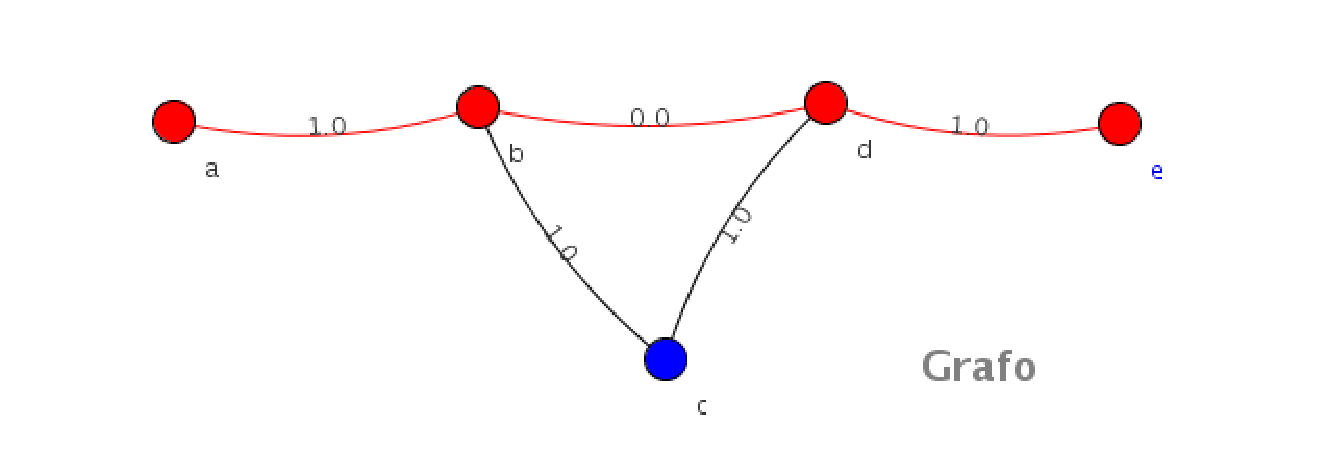
\includegraphics[scale=0.6]{./figs/grafoComZero.eps}
%% 
%% geramos as �rvores de menores caminhos, $T_a$, $T_e$ com ra�zes, respectivamente, $a$ e $e$:
%% 
%% 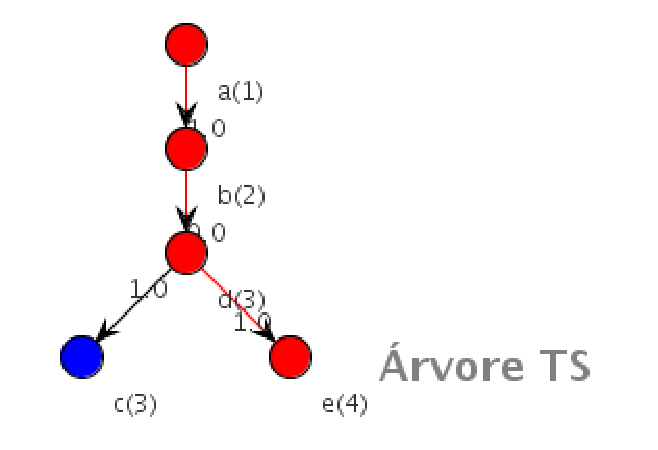
\includegraphics[scale=0.6]{./figs/arvoresTsComZero.eps}
%% 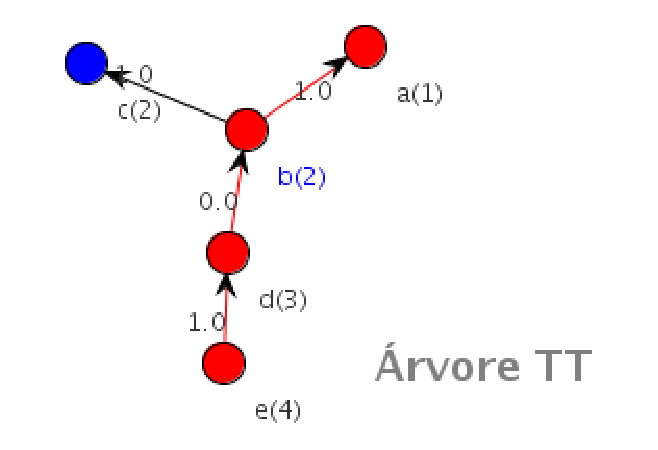
\includegraphics[scale=0.6]{./figs/arvoresTtComZero.eps}
%% 
%% Nas �rvores, a linha vermelha corresponde ao menor caminho de $a$ a $e$ e este � o mesmo que o 
%% destacado no grafo. 
%% 
%% Observe que $\epsilon(c) > \zeta(c)$( na �rvore $T_a$ $\epsilon(c)=3$ e na �rvore $T_e$ $\zeta(c)=2$)
%% violando a rela��o apresentada.
%% 
%% Com estas duas �rvores, o algoritmo n�o geraria nenhum caminho diferente de $\seq{a,b,d,e}$,
%% o que est� claramente incorreto, j� que existe o caminho $\seq{a,b,c,d,e}$.
%% 
%% %a partir do v�rtice $b$, o passeio do tipo II: 
%% %$a\underset{T_s}{\longrightarrow}b\underset{\in A}{\rightarrow}c \underset{T_t}{\longrightarrow}e = \seq{a,b,c,b,d,e}$ de custo 4,
%% %que n�o � um caminho, por conter v�rtices repetidos.
\newpage
\section{Simula��o}

Simularemos uma execu��o do algoritmo \KIM{} num grafo simples, exibindo passo a passo
as opera��es realizadas nas obten��es dos primeiros cinco caminhos.

Utilizaremos na nossa simula��o o grafo apresentado a seguir, no qual procuraremos
caminhos com ponta inicial no v�rtice $a$ e final em $i$. 

\includegraphics[scale=0.7]{./figs/simulacao/simulacao_grafo_1.eps}

Inicialmente, calculamos o menor caminho de $a$ a $i$, chamado de $P_1$, o qual est� destacado no grafo acima pelas arestas vermelhas.
A obten��o deste caminho resume-se a uma execu��o do algoritmo de Dijkstra no grafo apresentado.

Em seguida, a partir do caminho $P_1$, atrav�s da rotina \FSP{} calculamos o segundo menor caminho: $P_2$.
O caminho $P_2$ � o menor caminho de $a$ a $i$, que desvia do caminho $P_1$ em algum de seus v�rtices.
A gera��o de $P_2$ merece ser mais detalhada.

Primeiramente, s�o geradas duas �rvores de menores caminhos, chamadas respectivamente de $T_a$ e $T_i$.
A �rvore $T_a$ corresponde a �rvore de menores caminhos enraizada em $a$, devidamente rotulada com os valores de $\epsilon$ 
e contendo o caminho $P_1$.
A �rvore $T_i$ corresponde a �rvore de menores caminhos enraizada em $i$, devidamente rotulada com os valores de $\zeta$ 
e contendo o caminho reverso de $P_1$: $P_{1_r}$.

A seguir exibimos as �rvores $T_a$ e $T_i$ usadas na gera��o de $P_2$:
O r�tulo de cada v�rtice est� indicado pelo valor entre par�nteses. 
Os n�meros entre par�nteses da �rvore � esquerda correspondem aos 
valores de $\epsilon$ enquanto que os da direita aos de $\zeta$.

\includegraphics[scale=0.6]{./figs/simulacao/simulacao_ts_1.eps}
\includegraphics[scale=0.6]{./figs/simulacao/simulacao_tt_1.eps}

A partir dessas duas �rvores, a rotina \SEP{}, a qual � respons�vel 
por obter o menor caminho de $a$ a $i$ diferente de $P_1$, � chamada com $\alpha=6$, pois queremos um caminho
que desvia de $P_1$ antes do v�rtice $i$, cuja posi��o no caminho $P_1$ � 6.
A rotina \SEP{} examina os v�rtices da �rvore $T_a$ em profundidade, tentando obter caminhos dos tipos I e II, 
que desviem de $P_1$ antes do v�rtice $i$, retornando 
o de menor custo dentre eles.

Inicialmente adicionamos o v�rtice $a$ � pilha $S$ e definimos o custo atual do menor caminho encontrado at� o momento, $C$, 
como $\infty$. 
O conjunto $R$ armazena um v�rtice ou um arco\footnote{OS termos aresta e arco s�o intercambi�veis e podem ser usados 
sem preju�zo algum uma vez que estamos trabalhando com grafos sim�tricos.}, dependendo do tipo de caminho gerado.
Caso o caminho seja do tipo II ent�o $R$ armazenar� um v�rtice, se for tipo II ent�o armazenar� um arco.

Come�amos analisando o v�rtice $a$, para o qual temos:
$F_a=\{b\}, A_a=\{a,b\}$ e $\epsilon(a)=\zeta(a)$, j� que pertence ao caminho $P_1$.
Como $\epsilon(a)=\zeta(a)$ tentamos montar um caminho do tipo II, ou seja, um que fa�a uso de uma aresta n�o pertencente 
� �rvore $T_a$.
Procuramos todos os v�rtices vizinhos de $a$ no grafo e que n�o sejam vizinhos dele em $T_a$.
Neste caso n�o existe nenhum.
Adicionamos o �nico vizinho de $a$ em $T_a=\{b\}$ � $S$ e procedemos � pr�xima itera��o.

Seguimos analisando o v�rtice $b$, para o qual temos:
$F_b=\{c,e\}, A_b=\{a,c,e\}$ e $\epsilon(b)=\zeta(b)$, j� que pertence ao caminho $P_1$.
Tentamos, novamente, montar um caminho do tipo II e, para isso, procuramos todos os v�rtices 
vizinhos de $b$ no grafo que n�o sejam vizinhos dele em $T_a$, ou seja, $A_b-F_b=\{a\}$, mas
como $\epsilon(a)<\epsilon(b)$, temos que ignor�-lo. 
Observe que caso esta �ltima verifica��o n�o fosse feita, poder�amos gerar passeios que n�o fossem caminhos, 
por possu�rem v�rtices repetidos.
Empilhamos os v�rtices $c$ e $e$ e passamos � pr�xima itera��o.

Desempilhamos o v�rtice $e$, onde 
$F_e=\{d, f, h\}, A_e=\{b,d,f,h\}$ e $\epsilon(e)=\zeta(e)$.
Como $F_e-A_e=b$ e $\epsilon(b)<\epsilon(e)$ n�o temos nenhum v�rtice para analisar.
Empilhamos os v�rtices $d,f$ e $h$ em $S$. 
Observe que o v�rtice $b$ n�o � adicionado.

Desempilhamos o v�rtice $h$, obtendo $F_h=\emptyset, A_h=\{e,f,g\}$ e $\epsilon(h) \neq \zeta(h)$.
Tentamos agora montar um caminho do tipo I, concatenando o caminho $a\underset{T_a}{\longrightarrow}h$
ao $h\underset{T_i}{\longrightarrow}i$, formando um caminho de custo 5.
Uma vez que seu custo � menor que o menor custo atual fazemos: $R=h$ e $C=5$.

Desempilhamos o v�rtice $f$, onde $F_h=\emptyset$ e $\epsilon(f) \neq \zeta(f)$.
Montamos o caminho $a\underset{T_a}{\longrightarrow}f\underset{T_i}{\longrightarrow}i$, de custo 5.
Mantemos o caminho anterior, j� que o custo deste novo caminho n�o � inferior a 5.

Desempilhamos o v�rtice $d$, onde $F_d={g},A_d=\{c,e,f,g\}$ e $\epsilon(d)=\zeta(d)$.
Testamos apenas o $f$, uma vez que $\epsilon(c)<\epsilon(d)$ e $\epsilon(e)<\epsilon(d)$,
obtendo o caminho do tipo II: $a\underset{T_a}{\longrightarrow} d \rightarrow f \underset{T_i}{\longrightarrow} i$,
de custo 6. 
Empilhamos o v�rtice $g$.

Desempilhamos o v�rtice $g$, onde $F_g={i}, A_g=\{d,f,h,i\}$ e $\epsilon(g)=\zeta(g)$.

Desempilhamos o v�rtice $c$, onde $F_c=\emptyset, A_c=\{b,d\}$ e $\epsilon(c) \neq \zeta(c)$.
Montamos o caminho do tipo I: $a\underset{T_a}{\longrightarrow} c  \underset{T_i}{\longrightarrow} i$,
de custo 7.

A rotina \SEP{} � conclu�da com o caminho:  
$a\underset{T_a}{\longrightarrow}h\underset{T_i}{\longrightarrow}i$, cujo custo � 5.

Agora que acabamos de mostrar como o caminho $P_2$ � constru�do, vamos tratar da gera��o dos pr�ximos 
caminhos e exibir a estrutura dos caminhos $P_a,P_b$ e $P_c$.

At� o momento temos a seguinte �rvore de menores caminhos, formada pelos caminhos $P_1$ e $P_2$:

\includegraphics[scale=0.6]{./figs/simulacao/simulacao_paths_2_deitada.eps}

Onde o caminho $P_1$ � o que termina no n� $i_1$ e o caminho $P_2$ no $i_2$.
O �ltimo v�rtice comum aos caminhos $P_1$ e $P_2$ � o $e$, a partir do qual os caminhos se diferenciam.
O v�rtice $e$ desempenhar� um papel chave da gera��o dos caminhos derivados de $P_1$ e $P_2$ 
e ser� chamado v�rtice de desvio. 

Come�aremos pela gera��o do caminho $P_a$, o menor dentre todos os caminhos que desviam de $P_2$ ap�s o �ltimo v�rtice 
comum a $P_1$ e $P_2$.

Para a gera��o de $P_a$ necessitamos do �ltimo caminho gerado e de seu caminho gerador (pai), que
neste caso s�o, respectivamente, os caminhos: $P_2$ e $P_1$.

A id�ia � gerar o menor caminho de $h$ a $i$ e concaten�-lo ao prefixo comum aos caminhos $P_1$ e $P_2$ = $\seq{a,b,e}$.\\
Para evitar a gera��o de caminhos repetidos precisamos remover do grafo os v�rtices do prefixo comum
 e suas respectivas arestas: $\{(a,b),(b,e)\}$, obtendo o grafo:

\includegraphics[scale=0.6]{./figs/simulacao/simulacao_pa_1_grafo.eps}

A partir do novo grafo, oriundo dessas remo��es, executamos uma chamada � fun��o \FSP{}, utilizando 
$h$ como origem, $i$ como destino, o caminho base $P=\seq{h,g,i}$ e $\alpha=3$, obtendo as seguintes �rvores $T_h$ e $T_i$:

\includegraphics[scale=0.6]{./figs/simulacao/simulacao_pa_1_ts.eps}
\includegraphics[scale=0.6]{./figs/simulacao/simulacao_pa_1_tt.eps}

Por fim, a rotina \SEP{} � chamada retornando o caminho do tipo I: 
$h\underset{T_h}{\longrightarrow}f\underset{T_i}{\longrightarrow}i$ $=\seq{h,f,g,i}$,
de custo 3, o qual � concatenado ao prefixo $\seq{a,b,e}$ formando o caminho $P_a=\seq{a,b,e,h,f,g,i}$, de custo 6.

Na figura a seguir, temos os caminhos $P_1,P_2$ e $P_a$, com pontas iniciais $a$ e pontas finais, respectivamente : $i_1,i_2$ e $i_A$,
onde fica f�cil observar que o caminho $P_a$ desvia de $P_2$ ap�s o v�rtice $e$.
O caminho $P_a$ � filho do caminho $P_2$ o que est� indicado pelo n�mero entre colchetes no r�tulo 
da sua ponta final.

\includegraphics[scale=0.6]{./figs/simulacao/simulacao_pa_1_paths.eps}

Vamos agora tratar do caminho $P_b$, o menor caminho que desvia do caminho $P_1$
em algum ponto entre o v�rtice de desvio $e$ e o $i$. 
Para evitar a gera��o de caminhos repetidos precisamos excluir do grafo:
\begin{itemize}
\item Os v�rtices pertencentes ao prefixo comum aos caminhos $P_1$ e $P_2$ (excetuando-se o v�rtice de desvio), bem
como suas respectivas arestas. \\
Neste caso, os v�rtices a serem removidos s�o:$ \{a,b\}$ e as arestas $(a,b)$ e $(b,e)$.
\item As arestas com pontas nos v�rtices de desvio dos caminhos que t�m $P_1$ como pai.\\
No momento, o �nico caminho gerado a partir de $P_1$ � o $P_2$.\\
Observando-se a �rvore formada pelos menores caminhos encontrados at� o momento ($P_1$ e $P_2$), 
temos que aresta a ser removida � a $(e,h)$, pois tem ponta no v�rtice de desvio $e$ do caminho $P_2$ o
qual tem $P_1$ como pai.
\end{itemize}

Ap�s estas altera��es, obtemos o novo grafo, o qual possui o caminho $\seq{e,d,g,i}$ destacado:

\includegraphics[scale=0.6]{./figs/simulacao/simulacao_pb_1_grafo.eps}

Agora precisamos informar � rotina \FSP{} o valor de $\alpha$, para que ela saiba 
antes de qual v�rtice do caminho $\seq{e,d,g,i}$ o novo caminho tem que desviar.
Para a determina��o do $\alpha$ faremos o seguinte:
\begin{enumerate}
\item Tomaremos todos os caminhos gerados a partir de $P_1$ e seus respectivos v�rtices de desvio.\\
No momento o �nico caminho gerado a partir de $P_1$ � o $P_2$, cujo n� de desvio � o $e$;
\item Escolhemos o caminho que compartilha o menor prefixo com $P_2$, e que contenha o prefixo $\seq{a,b,e}$.
Ao v�rtice de desvio deste caminho daremos o nome de $\gamma$.
Caso $\gamma$ exista $\alpha=|\seq{e,\ldots,\gamma}|$.
Caso n�o exista $\alpha=|\seq{e,\ldots,i}|$
\end{enumerate}

No nosso caso, $\gamma$ n�o existe, logo $\alpha=|\seq{e,d,g,i}|=4$.

Executamos a rotina \FSP{} no novo grafo, utilizando o v�rtice $e$ como ponta inicial, $i$ como final, e $\alpha=4$,
obtendo as �rvores de menores caminhos $T_e$ e $T_i$ exibidas na figura a seguir:


\includegraphics[scale=0.6]{./figs/simulacao/simulacao_pb_1_ts.eps}
\includegraphics[scale=0.6]{./figs/simulacao/simulacao_pb_1_tt.eps}

Com as �rvores em m�os, a rotina \SEP{} retorna o menor caminho do tipo I:
$e\underset{T_e}{\longrightarrow}f\underset{T_i}{\longrightarrow}i=\seq{e,f,g,i}$.\\
Concatenando-o com o prefixo do caminho $P_1$: $\seq{a,b}$, obtemos o caminho $\seq{a,b,e,f,g,i}$, de custo 5.

A figura a seguir mostra a disposi��o do caminho $P_b$ calculado, o qual � representado pelo
caminho com ponta inicial em $a$ e final em $iB$:

\includegraphics[scale=0.6]{./figs/simulacao/simulacao_pb_1_paths.eps}

Entre colchetes vemos o n�mero 1, indicando que seu pai � o caminho $P_1$.

Vamos agora tratar do caminho $P_c$, o menor caminho que desvia do caminho $P_1$
em algum ponto antes do v�rtice de desvio $e$.

Dados todos os caminhos filhos de $P_1$, escolhemos aquele compartilha com $P_1$ o maior prefixo
e se desvia antes do v�rtice de desvio $e$.
Chamaremos de $\delta$ o v�rtice de desvio deste caminho com seu pai $P_1$.
Caso n�o exista, $\delta$ ser� igual � ponta inicial de $P_1$.
O $\alpha$ que ser� passado � fun��o \FSP{} e \SEP{}, corresponde
ao n�mero de v�rtices do subcaminho  de $P_1$ com ponta inicial em $\delta$ e ponta final em $e$.

Neste momento, $P_2$ � o �nico filho de $P_1$ e se desvia de $P_1$ no v�rtice $e$, logo $\delta=a$
 e $\alpha=|\seq{a,b,e}|=3$.
A fim de evitar a gera��o de caminhos repetidos, removemos do grafo
todas as arestas com pontas no v�rtice $\delta$ pertencentes aos caminhos filhos de $	P_1$.
Neste caso, n�o h� nenhuma aresta a ser removida

O grafo para c�lculo de $P_c$ � o pr�prio grafo original, onde o caminho $P_1$ est� destacado: 

\includegraphics[scale=0.6]{./figs/simulacao/simulacao_pc_1_grafo.eps}

Executamos a rotina \FSP{}, com ponta inicial $a$, ponta final $i$ e  $\alpha=3$, no grafo obtido, 
a qual nos retorna as seguintes �rvores $T_a$ e $T_i$:

\includegraphics[scale=0.6]{./figs/simulacao/simulacao_pc_1_ts.eps}
\includegraphics[scale=0.6]{./figs/simulacao/simulacao_pc_1_tt.eps}

Finalizamos chamando a rotina \SEP{} obtendo o caminho do tipo I: 
$a\underset{T_a}{\longrightarrow}c\underset{T_i}{\longrightarrow}i=\seq{a,b,c,d,g,i}$ de custo 7.
Observe que, como passamos $\alpha=3$, a rotina \SEP{} s� testou caminhos que desviavam antes do v�rtice $e$.
Nenhum v�rtice com $\epsilon>3$ foi adicionado � pilha $S$. 
Agora � poss�vel perceber a vantagem de se analisar os v�rtices da �rvore em profundidade.
Se tiv�ssemos analisado os v�rtice de qualquer maneira, ter�amos tentado gerar caminhos para 
muito mais v�rtices. 
O uso da pilha diminui isto, apenas os v�rtices $a$,$b$ e $c$ foram analisados.

A figura a seguir exibe os caminhos gerados at� o momento:

\includegraphics[scale=0.6]{./figs/simulacao/simulacao_pc_1_paths.eps}


Neste momento estamos com os caminhos candidatos: $P_a$, $P_b$ e $P_c$ e os menores caminhos: $P_1$ e $P_2$.
Retiramos o caminho de menor custo da lista de candidatos, neste caso $P_b$, 
e o adicionamos � lista de caminhos mais curtos, obtendo a seguinte 
�rvore de caminhos mais curtos:

\includegraphics[scale=0.6]{./figs/simulacao/simulacao_paths_3.eps}

Esses tr�s caminhos formar�o a base para a gera��o do 4� caminho mais curto.

Tomaremos o caminho $P_3$, cujo pai � $P_1$ e geraremos os caminhos $P_a,P_b$ e $P_c$, correspondentes.
O v�rtice de desvio desses dois caminhos � o $e$.

A gera��o de $P_a$ � relativamente simples.\\
Retiramos do grafo os v�rtices do prefixo comum a $P_1$ e $P_3$, ou seja, $\{a,b,e\}$, obtendo o grafo:

\includegraphics[scale=0.6]{./figs/simulacao/simulacao_pa_2_grafo.eps}

Executamos a fun��o \FSP{} com $\alpha=3$ para nos retornar o menor caminho de $f$ a $i$ diferente de $\seq{f,g,i}$, 
a qual nos retorna o caminho $\seq{f,h,g,i}$ atrav�s da execu��o do algoritmo \SEP{} nas �rvores:

\includegraphics[scale=0.6]{./figs/simulacao/simulacao_pa_2_ts.eps}
\includegraphics[scale=0.6]{./figs/simulacao/simulacao_pa_2_tt.eps}

Concatenamos o prefixo $\seq{a,b,e}$ ao caminho $\seq{f,h,g,i}$ obtendo o caminho $\seq{a,b,e,f,h,g,i}$, exibido
na figura a seguir:

\includegraphics[scale=0.6]{./figs/simulacao/simulacao_pa_2_paths.eps}

A gera��o de $P_b$ requer o c�lculo de um caminho que desvia de $P_1$ depois do v�rtice de desvio $e$ 
e seja diferente de todos os filhos de $P_1$.
Para isso, primeiro removemos os v�rtices do prefixo comum a $P_1$ e $P_3$ = $\seq{a,b,e}$ com exce��o do v�rtice $e$.
Depois, para evitar a gera��o de caminhos repetidos, apagamos as arestas: $(e,h)$ e $(e,f)$, obtendo o grafo:

\includegraphics[scale=0.6]{./figs/simulacao/simulacao_pb_2_grafo.eps}

Em seguida executamos rotina \FSP{}, com $s=e$, $t=i$ e $\alpha=4$, uma vez que n�o existe 
nenhum caminho filho de $P_1$ que desvia deste num v�rtice posterior a $e$.
Todos os caminhos gerados a partir de $P_1$, at� o momento, ou se desviam exatamente no v�rtice $e$ ou antes dele.
Obtemos ent�o as seguintes �rvores $T_e$ e $T_i$:

\includegraphics[scale=0.6]{./figs/simulacao/simulacao_pb_2_ts.eps}
\includegraphics[scale=0.6]{./figs/simulacao/simulacao_pb_2_tt.eps}

Por fim, a rotina \SEP{} nos devolve o caminho do tipo I: 
$e\underset{T_e}{\longrightarrow}f\underset{T_i}{\longrightarrow}i=\seq{e,d,f,g,i}$, que
concatenado ao $\seq{a,b,e}$ forma o caminho $\seq{a,b,e,d,f,g,i}$ de custo 7, exibido a seguir.

\includegraphics[scale=0.6]{./figs/simulacao/simulacao_pb_2_paths.eps}

N�o � poss�vel gerar nenhum caminho $P_c$ com base nos caminhos $P_1$ e $P_3$, pois
o menor caminho filho de $P_1$ que desvia antes do v�rtice de desvio $e$ j� foi calculado nas itera��es anteriores.

Retiramos da lista de candidatos o caminho de menor custo, ou seja, $\seq{a, b, e, d, f, g, i}$ e o inserimos
na lista de menores caminhos.
A �rvore dos menores caminhos, contendo os quatro menores caminhos se torna ent�o:

\includegraphics[scale=0.6]{./figs/simulacao/simulacao_paths_4.eps}

Para a gera��o do 5� caminho mais curto de $a$ a $i$ tomamos os caminhos: $P_4=\seq{a, b, e, d, f, g, i}$ e seu
caminho gerador: $P_1$.

Come�amos gerando um caminho na parti��o $P_a$.
O v�rtice de desvio entre $P_1$ e $P_4$ � o $d$.
Removemos do grafo os v�rtices do prefixo comum aos dois caminhos, bem como suas arestas correspondentes, obtendo o grafo:

\includegraphics[scale=0.6]{./figs/simulacao/simulacao_pa_3_grafo.eps}

A partir deste grafo resolvemos o problema do desvio de custo m�nimo, atrav�s da execu��o da rotina \SEP{} nas �rvores
de menores caminhos $T_f$ e $T_i$ e o caminho base $\seq{f,g,i}$:

\includegraphics[scale=0.6]{./figs/simulacao/simulacao_pa_3_ts.eps}
\includegraphics[scale=0.6]{./figs/simulacao/simulacao_pa_3_tt.eps}

A rotina \SEP{} nos retorna o desvio de custo m�nimo gerado a partir do v�rtice $h$: $\seq{f,h,g,i}$, um caminho
do tipo I: $f\underset{T_f}{\longrightarrow}h\underset{T_i}{\longrightarrow}i$.

O novo caminho na parti��o $P_a$ � obtido concatenando-se o prefixo $\seq{a,b,e,d}$ ao caminho $\seq{f,h,g,i}$,
obtendo-se o caminho: $\seq{a,b,e,d,f,h,g,i}$, exibido a seguir:
 
\includegraphics[scale=0.6]{./figs/simulacao/simulacao_pa_3_paths.eps}

Vamos tratar agora da gera��o do novo caminho na parti��o $P_b$.
Retiramos do grafo os v�rtices do prefixo comum, com exce��o do v�rtice de desvio, juntamente com suas arestas, ou
seja, apagamos os v�rtices: $\{a,b,e\}$ e as arestas: \\
$\{(a,b),(b,c),(b,e),(e,h),(e,f),(e,d)\}$.
Queremos ent�o obter um caminho na parti��o $P_b$ usando o desvio $d$ e gerar um que desvia de $P_1$ 
a partir deste v�rtice e que seja diferente.
Para evitar a gera��o de caminhos repetidos, � preciso remover algumas arestas. 
Vamos considerar todos os caminhos gerados a partir de $P_1$, com exce��o de $P_4$, 
que compartilham com este o menor prefixo tal que seja maior que o prefixo compartilhado entre $P_1$ e $P_4$, ou seja, 
queremos o caminho com menor prefixo tal este contenha o prefixo $\seq{a,b,e,d}$.
N�o h� nenhum caminho nestas condi��es.
Com isto, basta remover a aresta $(d, f)$ do grafo, evitando assim que o caminho $P_4$ venha ser novamente gerado.
A seguir o grafo com as altera��es mencionadas:

\includegraphics[scale=0.6]{./figs/simulacao/simulacao_pb_3_grafo.eps}

Pelo grafo � poss�vel perceber que n�o existe outro caminho de $d$ a $i$ 
diferente de $\seq{d,g,i}$. No entanto, vamos exibir as �rvores $T_d$ e $T_i$:

\includegraphics[scale=0.6]{./figs/simulacao/simulacao_pb_3_ts.eps}
\includegraphics[scale=0.6]{./figs/simulacao/simulacao_pb_3_tt.eps}

Vale notar que os v�rtices $\{c,f,h\}$ possuem $\epsilon=\zeta$, sem no entanto fazerem parte do caminho base $\seq{d,g,i}$.
Com tais �rvores o problema do desvio de custo m�nimo n�o tem solu��o.

Vamos passar para o caminho na parti��o $P_c$.
O representante da parti��o $P_c$ � um caminho de custo m�nimo que desvia de $P_1$ antes
do v�rtice de desvio $d$ e que n�o seja igual a nenhum dos filhos de $P_1$.

Olhando a �rvore de caminhos contendo os quatro primeiros caminhos observamos que os
gerados a partir de $P_1$ s�o: $P_2,P_3$ e $P_4$, cujos v�rtices de desvio s�o: $e,e$ e $d$.
Precisamos ent�o gerar o caminho com ponta em $e$ e que desvia de $P_1$ antes de $d$.
A escolha da ponta $e$ � como segue: escolha dos caminhos gerados a partir de $P_1$ aquele
que com este compartilhar o maior prefixo tal que seja menor que o prefixo comum a $P_1$ e $P_4$ e 
selecione o v�rtice de desvio deste caminho.
No nosso caso, o caminho escolhido � o $P_2$ cujo v�rtice de desvio � o $e$.

Exclu�mos do grafo as arestas com ponta no v�rtice de desvio $e$ e que perten�am aos filhos de $P_1$, 
ou seja, exclu�mos as arestas $\{(e,h),(e,f)\}$.
Al�m disso, � preciso remover os v�rtices do prefixo $\seq{a,b}$ juntamente com suas arestas.
O grafo oriundo destas altera��es �:

\includegraphics[scale=0.6]{./figs/simulacao/simulacao_pc_3_grafo.eps}

Geramos as �rvores $T_e$ e $T_i$, com o caminho base $\seq{e,d,g,i}$ e pedimos � fun��o \SEP{} que
nos retorne um desvio de custo m�nimo tal que o desvio ocorra antes do v�rtice $d$.
N�o existe tal caminho.

\includegraphics[scale=0.6]{./figs/simulacao/simulacao_pc_3_ts.eps}
\includegraphics[scale=0.6]{./figs/simulacao/simulacao_pc_3_tt.eps}

Retiramos da lista de candidatos um caminho de custo m�nimo, $\seq{a, b, e, h, f, g, i}$ e o adicionamos � lista
de menores caminhos que se torna:

\includegraphics[scale=0.6]{./figs/simulacao/simulacao_paths_5.eps}

O �ndice ap�s o $i$ corresponde � posi��o do caminho na lista de menores caminhos.
Por exemplo: $i1$ corresponde ao caminho $P_1$.
O n�mero entre colchetes se refere ao �ndice do pai do caminho.
Por exemplo: $i3[1]$ indica que o caminho $P_3$ foi gerado a partir do $P_1$.
A letra entre par�nteses indica a parti��o que este caminho representa.
Por exemplo: $i3[1](B)$ indica que o caminho $P_3$ � o representante da parti��o $P_b$ definida pelos 
caminhos $P_1$ e $P_3$.

\newpage
Todos os 17 caminhos gerados:

\includegraphics[scale=0.6]{./figs/simulacao/simulacao_all_paths.eps}

\newpage
\section{Implementa��o}
\label{sec:implementacao}
\subsection*{KIM}

A implementa��o foi feita em JAVA utilizando-se a biblioteca JUNG, mencionada anteriormente.
Nossa principal miss�o foi aproveitar ao m�ximo o c�digo j� existente no JUNG.
N�o exibiremos todo o c�digo nesta se��o, mas apenas pequenos trechos, com o intuito de explicar
como foi feita a implementa��o dos pontos que consideramos mais importantes.

Como j� dissemos, o algoritmo \KIM{} depende de uma rotina capaz de gerar uma �rvore de menores caminhos,
ou seja, uma rotina que resolva o problema $\PCM$, com algumas pequenas mudan�as, 
de forma a garantir a presen�a de um certo caminho, al�m das rotula��es $\epsilon$ e $\zeta$.

Atualmente a biblioteca JUNG possui apenas uma rotina que resolve o problema $\PCM$, utilizando o algoritmo de Dijkstra, implementado
usando uma fila de prioridade baseada num min-heap. Optamos ent�o por utiliz�-la.

De forma a garantir a presen�a de um certo caminho $P=\seq{u_1=s,\ldots,u_n=t}$ na �rvore de menores caminhos gerada pelo Dijkstra, 
permitimos que v�rtices que fazem parte do caminho sejam apenas alcan�ados por outros que tamb�m fa�am parte do caminho e,
al�m disso, sejam imediatamente anteriores a ele.
Lembrando do algoritmo de Dijkstra, apresentado na se��o~\ref{sec:dijkstra}, sempre que um arco est� sendo examinado,
ou seu v�rtice incidente est� em $Q$ ou n�o.
Se n�o estiver, deve ser inserido com o custo correspondente.
Se j� estiver, e o novo custo para alcan��-lo for inferior ao anteriormente calculado, devemos atualizar o seu custo.
A a��o de inserir um v�rtice em $Q$ est� mapeada na fun��o \lstinline{createRecord(V w, E e, double new_dist)} apresentada no c�digo a seguir.
Observe que, caso o v�rtice, do arco incidente atualmente sendo examinado, n�o esteja em $P$ nada de especial precisa ser feito, 
mas caso contr�rio precisamos garantir que seu predecessor seja um v�rtice pertencente � $P$ e, imediatamente anterior a este em $P$.
Para testar que est� no caminho basta verificar os retornos das chamadas da fun��o \lstinline{isOnPath}, nas linha~5 e 6.
A fim de testar que seja imediatamente anterior, subtra�mos os valores das rotula��es entre os dois v�rtices em quest�o.
Caso estejamos gerando a �rvore de menores caminhos $T_s$, utilizamos a rotula��o $\epsilon$, sen�o utilizamos a $\zeta$.
\begin{lstlisting}
protected class SourcePathDataKIM extends SourcePathData {
	@Override
	public void createRecord(V w, E e, double new_dist) {
		V pred = ((UndirectedGraph<V, E>) g).getOpposite(w, e);
		if (w.isOnPath()) {
			if (!pred.isOnPath())
				return;
			if (getTreeType().equals(ShortestPathKIM.TreeType.TS)) {
				if (w.getEpsilon().intValue()-pred.getEpsilon().intValue() != 1)
					return;
			} else if (getTreeType().equals(ShortestPathKIM.TreeType.TT)) {
				if (w.getZeta().intValue()-pred.getZeta().intValue() != -1)
					return;
			}
		}
		super.createRecord(w, e, new_dist);
	}
}
\end{lstlisting}

Ainda temos o problema das rotula��es para resolver.
Vale lembrar que:

Sejam $T_s$ e $T_t$ duas �rvores de menores caminhos com ra�zes $s$ e $t$, respectivamente, 
geradas a partir de execu��es do \PCM{} no grafo sim�trico com custo $(V,A,c)$ e 
$P=\seq{s,\ldots,t}$ o caminho base em $T_s$ ent�o:

$\forall u \in V, u \in T_s, u \in P \rightarrow \epsilon(u)=\zeta(u)=|prefixo(\seq{s,\ldots,u})|$

$\forall u \in V, u \in T_s, u \notin P \rightarrow \epsilon(u)=\epsilon(\pred_{T_s}(u))$

$\forall u \in V, u \in T_t, u \notin P \rightarrow \zeta(u)=\zeta(\pred_{T_t}(u)$

Sendo assim, definimos a fun��o de rotula��o como exibida no c�digo a seguir.

\begin{lstlisting}
	private void setLabel(V w, V pred) {
		if (!w.isOnPath()) {
			if (getTreeType().equals(ShortestPathKIM.TreeType.TS))
				w.setEpsilon(pred.getEpsilon());
			else if (getTreeType().equals(ShortestPathKIM.TreeType.TT))
				w.setZeta(pred.getZeta());
		}
\end{lstlisting}
Observe que rotulamos apenas os v�rtices n�o pertencentes ao caminho $P$.
A rotula��o dos v�rtices em $P$ � feita em um momento anterior ao da execu��o do algoritmo \PCM{} modificado.
Antes de todas as chamadas a fun��o \FSP{}, executamos a rotina \lstinline{insertPathOnTree}, apresentada a seguir.
\begin{lstlisting}
protected void insertPathOnTree(Path<KIMVertex, KIMEdge> path, int ini) {
	for (int i = ini, epsilon = 1; i < path.getVertices().size(); i++, epsilon++) {
		KIMVertex atual = path.getVertex(i);
		atual.setIsOnPath(true);
		atual.setEpsilon(epsilon);
		atual.setZeta(epsilon);
	}
}
\end{lstlisting}
O seu c�digo � bem simples e nada mais faz que aplicar a defini��o das rotula��es $\epsilon$ e $\zeta$ aos v�rtices pertencentes ao caminho $P$. 

Agora precisamos definir quando as rotula��es dos v�rtices n�o pertencentes � $P$ devem ser feitas.
Observamos que sempre que um v�rtice � adicionado a $S$ podemos, seguramente, rotul�-lo, uma vez que seu predecessor n�o mais mudar�.
\begin{lstlisting}
@Override
	public Entry<V, Number> getNextVertex() {
		Map.Entry<V, Number> p = super.getNextVertex();
		V v = p.getKey();
		E incomingEdge = incomingEdges.get(v);
		if (incomingEdge != null) {
			V pred = ((UndirectedGraph<V, E>) g).getOpposite(v, incomingEdges.get(v));
			setLabel(v, pred);
			sons.get(pred).add(v);
		}
		sons.put(v, new LinkedHashSet<V>());
		return p;
	}
\end{lstlisting}

O c�digo completo da classe que implementa as estruturas de dados utilizadas no algoritmo \PCM{} modificado � apresentada a seguir:
\begin{lstlisting}[name={Estruturas de dados da implementa��o do algoritmo Dijkstra modificado.}]
	protected class SourcePathDataKIM extends SourcePathData {
		@Override
		public Entry<V, Number> getNextVertex() {
			Map.Entry<V, Number> p = super.getNextVertex();
			V v = p.getKey();
			E incomingEdge = incomingEdges.get(v);
			if (incomingEdge != null) {
				V pred = ((UndirectedGraph<V, E>) g).getOpposite(v, incomingEdges.get(v));
				setLabel(v, pred);
				sons.get(pred).add(v);
			}
			sons.put(v, new LinkedHashSet<V>());
			return p;
		}

		@Override
		public void createRecord(V w, E e, double new_dist) {
			V pred = ((UndirectedGraph<V, E>) g)
					.getOpposite(w, e);
			if (w.isOnPath()) {
				if (!pred.isOnPath())
					return;
				if (getTreeType().equals(ShortestPathKIM.TreeType.TS)) {
					if (w.getEpsilon().intValue()-pred.getEpsilon().intValue() != 1)
						return;
				} else if (getTreeType().equals(ShortestPathKIM.TreeType.TT)) {
					if (w.getZeta().intValue()-pred.getZeta().intValue() != -1)
						return;
				}
			}
			super.createRecord(w, e, new_dist);
		}

		private void setLabel(V w, V pred) {
			if (!w.isOnPath()) {
				if (getTreeType().equals(ShortestPathKIM.TreeType.TS))
					w.setEpsilon(pred.getEpsilon());
				else if (getTreeType().equals(ShortestPathKIM.TreeType.TT))
					w.setZeta(pred.getZeta());
			}
		}

		public SourcePathDataKIM(V source) {
			super(source);
		}
	}
\end{lstlisting}

Achamos importante tratar de um detalhe da fun��o \SEP{}, � qual implementa o algoritmo \SEP{} apresentado anteriormente.
Na linha~5 do algoritmo temos a defini��o de $F_u$ como o conjunto de v�rtices em $T_s$ cujo predecessor seja o v�rtice $u$.
O problema � que temos em m�os apenas a �rvore de menores caminhos, na forma de um grafo de  predecessores.
Para obter o conjunto $F_u$, a partir da �rvore de menores caminhos, usamos o c�digo a seguir, o qual dada uma �rvore de menores caminhos \lstinline{T},
um v�rtice \lstinline{u} e um v�rtice \lstinline{s} tal que $\pred_{T}(s)=\emptyset$, retorna os filhos de \lstinline{u} na �rvore 
\lstinline{T} com raiz \lstinline{s}:
\begin{lstlisting}
protected Set<KIMVertex> getSons(ShortestPathKIM<KIMVertex, KIMEdge> T,
											KIMVertex u, KIMVertex s) {
		Iterator<KIMEdge> i = graph.getOutEdges(u).iterator();
		Set<KIMVertex> sons = new HashSet<KIMVertex>();
		while (i.hasNext()) {
			KIMEdge atual = i.next();
			KIMVertex o = graph.getOpposite(u, atual);
			KIMEdge incident = T.getIncomingEdge(s, o);
			if (incident != null	&& graph.getOpposite(o, incident).equals(u))
				sons.add(o);
		}
		return sons;
	}
\end{lstlisting}
O c�digo anterior exige que todas as arestas de \lstinline{u} sejam testadas quanto a sua exist�ncia na �rvore \lstinline{T}, ocasionando um 
consumo de tempo $\Oh(m)$.
Descobrimos, posteriormente, que poder�amos armazenar, para cada v�rtice  \lstinline{u}, seu conjunto $F_u$ durante
a execu��o do algoritmo $\PCM$ modificado.
Observamos que sempre que um novo v�rtice � adicionado ao conjunto $S$, uma vez que seu predecessor n�o mais mudar�, 
podemos adicion�-lo � lista de filhos de seu predecessor.
O c�digo a seguir resume o que foi dito.
\begin{lstlisting}
		public Entry<V, Number> getNextVertex() {
			Map.Entry<V, Number> p = super.getNextVertex();
			V v = p.getKey();
			E incomingEdge = incomingEdges.get(v);
			if (incomingEdge != null) {
				V pred = ((UndirectedGraph<V, E>) g).getOpposite(v, incomingEdges.get(v));
				setLabel(v, pred);
				sons.get(pred).add(v);
			}
			sons.put(v, new LinkedHashSet<V>());
			return p;
		}
\end{lstlisting}
Na linha~8 obtemos a lista de filhos do v�rtice predecessor e lhe adicionamos o novo v�rtice \lstinline{v}.
Na linha~10 criamos a lista de filhos do v�rtice \lstinline{v}.
Aplicando esta mudan�a conseguimos ganhos de desempenho de at� 40\%.
Notamos que quanto maior for a densidade de um grafo tanto mais tempo gastaremos executando a rotina \lstinline{getSons}.

Decidimos implementar uma solu��o para o $\PCM$ modificado quando a fun��o custo � constante.
Quando a fun��o custo � constante, uma simples busca em largura � suficiente para retornar as �rvores de menores caminhos a partir da origem.
O JUNG possu�a uma implementa��o para grafos sem custos, no entanto, uma vez que o c�digo e as estruturas estavam juntas, n�o
conseguimos reaproveit�-lo, pois precis�vamos alter�-lo com as rotula��es e a presen�a do caminho base.

Utilizando busca em largura, garantir que um certo caminho base fa�a parte da �rvore gerada pode ser realizado 
for�ando cada v�rtice do caminho a ser analisado apenas pelo v�rtice anterior a ele no caminho.
Observa que isso � feito nas linhas~16 e 17 quando impedimos que o v�rtice \lstinline{neighbor} entre para $\Scal$
caso ele fa�a parte do caminho base e o v�rtice \lstinline{cur} n�o.

Veja que nas linhas~25 a 32 as rotula��es $\epsilon$ e $\zeta$ s�o feitas de acordo com a defini��o apresentada anteriormente.
Mais uma vez, apenas rotulamos, na implementa��o do algoritmo $\PCM$, v�rtices que n�o fa�am parte do caminho.
Os v�rtices que fazem parte do caminho s�o rotulados num momento anterior.

\begin{lstlisting}
	private void bfs(KIMVertex source) {
		LinkedList<KIMVertex> unknown = new LinkedList<KIMVertex>();
		distanceMap = new HashMap<KIMVertex, Number>();
		incomingEdgeMap = new HashMap<KIMVertex, KIMEdge>();
		unknown.add(source);
		distanceMap.put(source, 0);
		while (!unknown.isEmpty()) {
			KIMVertex cur = unknown.pollFirst();
			Iterator<KIMEdge> i = g.getIncidentEdges(cur)
					.iterator();
			while (i.hasNext()) {
				KIMEdge incomingEdge = i.next();
				KIMVertex neighbor = g.getOpposite(cur,
						incomingEdge);
				if (!distanceMap.containsKey(neighbor)
						&& !(neighbor.isOnPath() && !cur
								.isOnPath())) {
					unknown.addLast(neighbor);
					incomingEdgeMap.put(neighbor,
							incomingEdge);
					distanceMap
							.put(neighbor,
									(Integer) distanceMap
											.get(cur) + 1);
					if (!neighbor.isOnPath()
							&& treeType != null) {
						if (treeType.equals(ShortestPathKIM.TreeType.TS))
							neighbor.setEpsilon(cur
									.getEpsilon());
						else if (treeType
								.equals(ShortestPathKIM.TreeType.TT))
							neighbor.setZeta(cur.getZeta());
					}
				}
			}
		}
	}
\end{lstlisting}

Tendo as duas implementa��es para o \PCM{} modificado: uma baseada no algoritmo de Dijkstra e utilizando grafos com custo n�o-negativos
e outra baseada numa simples busca em largura e lidando com grafos com custos constantes, era preciso fornecer uma maneira de 
utiliz�-los de uma maneira uniforme pelo algoritmo \KIM{}.
Para isso, inicialmente definimos a interface \lstinline{ShortestPathKIM}:
\begin{lstlisting}
public interface ShortestPathKIM<V extends KIMVertex, E extends KIMEdge>
		extends ShortestPath<V, E>, Distance<V> {
	public static final Class BFSShortestPathKIMAlgorithm = BFSKIM.class;
	public static final Class DijkstraShortestPathKIMAlgorithm = DijkstraSPKIM.class;

	public List<E> getPath(V source, V target);

	public E getIncomingEdge(V source, V target);

	public LinkedHashSet<V> getSons(V source, V vertex);
}
\end{lstlisting}
Assim, toda classe utilizada para resolver o \PCM{} modificado durante a execu��o do algoritmo \KIM{} deveria 
implementar os m�todos definidos por essa interface.
Al�m disso, criamos uma f�brica de inst�ncias do \PCM{} modificado, para facilitar nas suas cria��es.
\begin{lstlisting}
public class Factory {
		Transformer<KIMEdge, Number> nev;
		UndirectedGraph<KIMVertex, KIMEdge> g;
		Class shortestPathKIM;
		public Constructor construtor;

		public Factory(Transformer<KIMEdge, Number> nev,
				UndirectedGraph<KIMVertex, KIMEdge> g,
				Class<ShortestPathKIM<KIMVertex, KIMEdge>> shortestPathKIM) {
			this.nev = nev;
			this.g = g;
			this.shortestPathKIM = shortestPathKIM;
			try {
				construtor = shortestPathKIM.getConstructor(new Class[] {
						UndirectedGraph.class, Transformer.class,
						ShortestPathKIM.TreeType.class });
			} catch (Exception e) {
				RuntimeException err = new RuntimeException();
				err.initCause(e);
				throw err;
			}
		}

		public ShortestPathKIM<KIMVertex, KIMEdge> newInstance(
				ShortestPathKIM.TreeType treeType) {
			try {
				return (ShortestPathKIM<KIMVertex, KIMEdge>) construtor
						.newInstance(new Object[] { g, nev, treeType });
			} catch (Exception e) {
				RuntimeException err = new RuntimeException();
				err.initCause(e);
				throw err;
			}
		}
	}
\end{lstlisting}

O construtor da classe \KIM {} recebe uma f�brica de inst�ncias do \PCM{} modificado e uma fun��o custo na forma de um \emph{Transformer} conseguindo
resolver o problema \kCM{} sem se preocupar com a implementa��o do \PCM{} modificado informada.

Precisamos criar classe espec�ficas para v�rtices e arestas, uma vez que desej�vamos armazenar informa��es espec�ficas 
relativas ao algoritmo \KIM{}. Nossa classe \lstinline{KIMVertex} possui dois campos que armazenam os valores das rotula��es $\epsilon$ e $\zeta$,
uma vari�vel \lstinline{boolean} chamada \lstinline{isOnPath} usada para indicar se o v�rtice faz parte do caminho base ou n�o e, 
para depura��o do c�digo, adicionamos um campo \lstinline{nome}.
Para facilitar nas leituras de grafos a partir de arquivos \emph{PajekNet} adicionamos � classe uma f�brica padr�o de v�rtices.
\begin{lstlisting}
public class KIMVertex {
	public static class KIMVertexFactory implements Factory<KIMVertex> {
		int id = 1;
		@Override
		public KIMVertex create() {
			return new KIMVertex(Integer.toString(id++));
		}
	}
	public static Factory<KIMVertex> getFactory() {
		return new KIMVertex.KIMVertexFactory();
	}
	private Integer epsilon;
	private boolean isOnPath = false;
	private String nome;
	private Integer zeta;

	public KIMVertex(String nome) {
		this(nome, false);
	}
	public KIMVertex(String nome, boolean isOnPath) {
		this.nome = nome; this.isOnPath = isOnPath;
	}
	@Override
	public boolean equals(Object obj) {
		if (obj == null)
			return false;
		try {
			KIMVertex other = (KIMVertex) obj;
			return getNome().equals(other.getNome());
		} catch (ClassCastException e) { return false;}
	}
}
\end{lstlisting}
Os m�todos \lstinline{get} e \lstinline{set} para cada campo foram suprimidos na listagem anterior, por conveni�ncia.

A nossa classe \lstinline{KIMEdge} possui um campo para armazenar um custo, uma f�brica padr�o de arestas e duas fun��es custos mapeadas nos 
\lstinline{Transformers}: \lstinline{defaultCost} e \lstinline{constantCost}.
A seguir o c�digo da classe \lstinline{KIMEdge}:

\begin{lstlisting}
public class KIMEdge {
	@Override
	public boolean equals(Object obj) {
		if (obj == null)
			return false;
		try {
			return ((KIMEdge) obj).getID().equals(myID);
		} catch (ClassCastException e) {return false;}
	}
	private static int id;
	private static Transformer<KIMEdge, Number> defaultCost = new Transformer<KIMEdge, Number>() {
		public Number transform(KIMEdge link) {
			return link.getCost();
		}
	};
	private static Transformer<KIMEdge, Number> constantCost = new Transformer<KIMEdge, Number>() {
		public Number transform(KIMEdge link) {
			return 1;
		}
	};
	private int myID;
	@Override
	public String toString() {
		return "[E" + myID + "," + cost + "]";
	}
	private Number cost;
	public KIMEdge() {
		this(null);
	};
	public KIMEdge(Number cost) {
		synchronized (KIMEdge.class) {
			id++;
			this.myID = id;
		}
		this.cost = cost;
	}
	public static final Transformer<KIMEdge, Number> getDefautTransformer() {
		return defaultCost;
	}
	public static final Transformer<KIMEdge, Number> getConstantTransformer() {
		return constantCost;
	}
	public static class KIMEdgeFactory implements Factory<KIMEdge> {
		@Override
		public KIMEdge create() {
			return new KIMEdge();
		}
	}
	public static Factory<KIMEdge> getFactory() {
		return new KIMEdge.KIMEdgeFactory();
	}
}
\end{lstlisting}
Alguns \emph{getters} e \emph{setters} foram omitidos.

N�o havia no JUNG uma classe que representasse a id�ia de caminho.
Para o JUNG um caminho era sempre uma lista de arcos e/ou arestas.
N�s precisamos armazenar outras informa��es, como por exemplo, o caminho pai, o v�rtice de desvio, o custo, entre outros.
Al�m disso, dado que a rotina \SEP{} retorna ora um v�rtice ora um arco, seria interessante que a nossa classe 
soubesse criar um caminho com base nestas duas op��es.
A seguir exibimos um excerto da interface \lstinline{Path}.
\begin{lstlisting}
public interface Path<V extends KIMVertex, E extends KIMEdge> {
	public abstract int getIteracao();
	public abstract void setIteracao(int iteracao);
	public abstract Double getCost();
	public abstract KIMVertex getDevVertex();
	public abstract int getDevNodeIndex();
	public abstract KIMEdge getEdge(int pos);
	public abstract List<KIMEdge> getEdges();
	public abstract int getOrdem();
	public abstract String getOrigem();
	public abstract Path<KIMVertex, KIMEdge> getParent();
	public abstract Path<KIMVertex, KIMEdge> getPrefix(KIMVertex last);
	public abstract Path<KIMVertex, KIMEdge> getReverse();
	public abstract KIMVertex getStart();
	public abstract Path<KIMVertex, KIMEdge> getSubPath(KIMVertex v);
	public abstract Path<KIMVertex, KIMEdge> getSubPath(KIMVertex v, int from,
			int to);
	public abstract KIMVertex getTarget();
	public abstract KIMVertex getVertex(int pos);
	public abstract List<KIMVertex> getVertices();
	public abstract void setOrdem(int ordem);
	public abstract void setOrigem(String origem);
	public abstract void setParent(Path<KIMVertex, KIMEdge> parent);
	public class Factory {
		private UndirectedGraph<KIMVertex, KIMEdge> g;
		public UndirectedGraph<KIMVertex, KIMEdge> getGraph() {
			return g;
		}
		public Transformer<KIMEdge, Number> getTransformer() {
			return nev;
		}

		private Transformer<KIMEdge, Number> nev;

		public Factory(UndirectedGraph<KIMVertex, KIMEdge> g,
				Transformer<KIMEdge, Number> nev) {
			this.g = g;
			this.nev = nev;
		}

		public final Path<KIMVertex, KIMEdge> newInstance(
				Path<KIMVertex, KIMEdge> p1, Path<KIMVertex, KIMEdge> p2) {
			return new BasicPath<KIMVertex, KIMEdge>(p1, p2, g, nev);
		}

		public final Path<KIMVertex, KIMEdge> newInstance(List<KIMEdge> edges,
				KIMVertex vertex) {
			return new BasicPath<KIMVertex, KIMEdge>(edges, vertex, g, nev);
		}

		public final Path<KIMVertex, KIMEdge> newInstance(
				ShortestPathKIM<KIMVertex, KIMEdge> Ts,
				ShortestPathKIM<KIMVertex, KIMEdge> Tt, Pair pair, KIMVertex s,
				KIMVertex t) {
			return new BasicPath<KIMVertex, KIMEdge>(Ts, Tt, pair, s, t, g, nev);
		}
	}
}
\end{lstlisting}
Boa parte dos m�todos definidos nas linhas~2 a 15 corresponde a campos utilizados para prop�sito de depura��o.
Na linha~25 vemos a defini��o de uma f�brica de \lstinline{Path} que armazena um grafo e uma fun��o custo mapeada na forma de um \lstinline{Transformer}.
A f�brica utiliza essas informa��es para gerar caminhos 	de diversas maneiras, dentre as quais destacamos:
\begin{description}
\item[linha~41]: a partir da concatena��o de dois caminhos;
\item[linha~51]: a partir das �rvores $T_s$ e $T_t$, $s$ e $t$ e um \lstinline{pair} que ora representa uma aresta ora um v�rtice.
A implementa��o deve gerar um caminho do tipo I quando \lstinline{pair} contiver dois v�rtices iguais e caminhos do tipo II
quando forem diferentes.
\end{description} 

As demais rotinas n�o valem a pena de serem exibidas e lembramos que o c�digo implementado pode ser baixado no
s�tio: http://code.google.com/p/k-cmc/.


\chapter{Resultados Experimentais}
\label{cap:experimentos}
\longpage
\section{Motiva��o}
  Recentemente, h� um grande interesse em trabalhos relacionados a
  an�lise experimental de algoritmos. 
  Em particular, no caso do
  algoritmo \Dijkstra{}, uma subrotina do algoritmo \KIM{}, podemos citar os artigos de B.V.~Cherkassky,
  A.V.~Goldberg, T.~Radzik e Craig Silverstein 
  ~\cite{boris:experimental, goldberg:buckets, boris:buckets},
   e do algoritmo \KIM{}
  podemos citar o artigo de Eleni Hadjiconstantinou and Nicos Christofides~\cite{eleni:n-34-88}.

  O interesse em experimenta��o � devido ao reconhecimento de que os
resultados te�ricos, freq�entemente,
  n�o trazem informa��es referentes ao desempenho do algoritmo na
  pr�tica. Por�m, o campo da an�lise experimental � repleto de
  armadilhas, como comentado por
  D.S.~Johnson~\cite{johnson:guide}. Muitas vezes, a implementa��o do
  algoritmo � a parte mais simples do experimento. A parte dif�cil � usar, 
  com sucesso, a implementa��o para produzir resultados de pesquisa significativos.

  Segundo D.S.~Johnson~\cite{johnson:guide}, pode-se dizer que existem
  quatro motivos b�sicos que levam a realizar
  um trabalho de implementa��o de um algoritmo:
  \begin{enumerate}[(1)]
  \item Para usar o c�digo em uma aplica��o particular, cujo prop�sito
  � descrever o impacto do algoritmo em um certo contexto;
  \item Para proporcionar evid�ncias da superioridade de um algoritmo;
  \item Para melhor compreens�o dos pontos fortes, fracos e do 
  desempenho das opera��es algor�tmicas na pr�tica; e 
  \item Para produzir conjecturas sobre o comportamento do algoritmo
  no caso-m�dio sob distribui��es espec�ficas de inst�ncias onde a
  an�lise probabil�stica direta � muito dif�cil.
  \end{enumerate}
  Nesta disserta��o estamos mais interessados no motivo (3).
  
\section{Ambiente experimental}
Nos experimentos utilizamos duas plataformas:
\begin{enumerate}
\item[\iten{1}] Um servidor Linux 32 bits com 4 processadores Intel Pentium 4 Xeon 3,39MHz e 3,5 GB de RAM;
\item[\iten{2}] Um notebook rodando Linux Ubuntu 8.04, Kernel 2.6.24-23 com dois processadores Intel T7500 de 2.20Ghz e 2GB de RAM.
\end{enumerate}

Os experimentos das se��es~\ref{sec:tempo_x_k}, \ref{sec:tempo_x_densidade}, \ref{sec:tempo_x_n} e \ref{sec:sep_fsp} 
foram executados na plataforma~\iten{1}, enquanto que os demais na \iten{2}.
Como o que nos interessa n�o � especificamente o tempo absoluto de execu��o, mas a curva do tempo de execu��o,
acreditamos que essa mudan�a de plataforma n�o chega a alterar nossos resultados.

Para controlar os tempos usamos a classe \lstinline{StopWatch}, implementada por Rod Johnson e Juergen Hoeller:
\lstset{tabsize=2,caption=,numbers=left, numberstyle=\tiny, stepnumber=1, numbersep=5pt,basicstyle=\footnotesize,showstringspaces=false}
\begin{lstlisting}[name=Classe usada no controle dos tempos de execu��o,label=stopwatch]
public class StopWatch {
	private final String id;
	private boolean keepTaskList = true;
	private final List taskList = new LinkedList();
	private long startTimeMillis;
	private boolean running;
	private String currentTaskName;
	private TaskInfo lastTaskInfo;
	private int taskCount;
	private long totalTimeMillis;

	public StopWatch() {
		this.id = "";
	}

	public StopWatch(String id) {
		this.id = id;
	}

	public void start(String taskName) throws IllegalStateException {
		if (this.running) {
			throw new IllegalStateException(
					"Can't start StopWatch: it's already running");
		}
		this.startTimeMillis = System.currentTimeMillis();
		this.running = true;
		this.currentTaskName = taskName;
	}

	public void stop() throws IllegalStateException {
		if (!this.running) {
			throw new IllegalStateException(
					"Can't stop StopWatch: it's not running");
		}
		long lastTime = System.currentTimeMillis() - this.startTimeMillis;
		this.totalTimeMillis += lastTime;
		this.lastTaskInfo = new TaskInfo(this.currentTaskName, lastTime);
		if (this.keepTaskList) {
			this.taskList.add(lastTaskInfo);
		}
		++this.taskCount;
		this.running = false;
		this.currentTaskName = null;
	}

	public long getLastTaskTimeMillis() throws IllegalStateException {
		if (this.lastTaskInfo == null) {
			throw new IllegalStateException(
					"No tests run: can't get last interval");
		}
		return this.lastTaskInfo.getTimeMillis();
	}

	public long getTotalTimeMillis() {
		return totalTimeMillis;
	}
}

\end{lstlisting}

O uso da classe \lstinline{StopWatch} � bem simples. 
Eis um pequeno exemplo:
\lstset{caption=,numbers=left, numberstyle=\tiny, stepnumber=1, numbersep=5pt,label=stopwatchsample,nolol=true}
\begin{lstlisting}
	StopWatch stopWatch = new StopWatch("KIM");
	stopWatch.start();
	/*Aqui vai a chamada � tarefa cuja tempo deseja-se medir*/
	stopWatch.stop();
	int time = stopWatch.getLastTaskTimeMillis();
\end{lstlisting}
Na linha~1 criamos uma inst�ncia da classe.
Em seguida, na linha 2, inicializamos o cron�metro.
Na linha 3 fica a chamada � fun��o cujo tempo ser� medido.
Paramos o cron�metro na linha 4 e chamamos o m�todo \lstinline{getLastTaskTimeMillis()} para obter o tempo decorrido.

Para calcular o uso de mem�ria utilizamos o seguinte trecho de c�digo:
\begin{lstlisting}[name=C�lculo do consumo de mem�ria,caption={}]
	long initMem = Runtime.getRuntime().freeMemory();
	/* leitura ou geracao do grafo */
	long graphMemUsage = initMem - Runtime.getRuntime().freeMemory();
	// execu��o do algoritmo
	long kimMemUsage = initMem - graphMemUsage - Runtime.getRuntime().freeMemory();
\end{lstlisting}
Na linha 1 a quantidade de mem�ria livre do sistema � armazenada na vari�vel \lstinline{initMem}.
Na linha 3, ap�s a leitura e armazenamento do grafo em mem�ria, guardamos a mem�ria consumida pelo grafo.
Executamos, em seguida, o nosso algoritmo e por fim, na linha 5, calculamos a diferen�a entre a quantidade inicial de mem�ria livre 
e as quantidades de mem�ria consumidas pelo grafo e pelo algoritmo.

Os testes foram criados levando-se em conta o consumo de tempo assint�tico do algoritmo \KIM{}, $\Theta(kT(n,m))$, 
onde $T(n,m)$ � o consumo de tempo da subrotina que calcula uma �rvore de 
menores caminhos. No caso de grafos sem custos nas arestas, utilizamos uma busca em largura, cuja consumo de tempo
� $\Theta(n + m)$, caso contr�rio utilizamos a implementa��o do Dijkstra feita no JUNG (se��o \ref{sec:dijkstraJUNG}), 
cujo consumo � $\Theta(m \log n)$.
Nos testes realizados, utilizamos apenas a implementa��o do Dijkstra feita no JUNG.

\section{Gerador de inst�ncias}
Implementamos um pequeno gerador de grafos sim�tricos aleat�rios utilizando a interface \lstinline{GraphGenerator} 
fornecida pelo JUNG.
Inicialmente pensamos em utilizar geradores dispon�veis na DIMACS, mas estes geravam apenas grafos,
desta maneira ter�amos que convert�-los para grafos sim�tricos.
O gerador implementado segue a id�ia apresentada no artigo de Eleni Hadjiconstantinou and Nicos Christofides~\cite{eleni:n-34-88}:
\begin{enumerate}[(1)]
\item Inicialmente criamos os v�rtices;
\item Em seguida, produzimos um ciclo hamiltoniano ligando cada v�rtice ao seu vizinho, garantindo assim 
que o grafo gerado seja conexo;
\item Finalizamos adicionando, aleatoriamente, o restante dos arestas. 
\end{enumerate}

Na cria��o dos grafos aleat�rios utilizamos os seguintes par�metros: 
\begin{itemize}
\item $n$ n�mero de v�rtices;
\item $m$ n�mero de arestas, sendo que $n \leq m \leq n(n-1)/2$, pois se $m < n$ n�o � poss�vel construir o ciclo hamiltoniano e, 
se $m > n(n-1)/2$ n�o � poss�vel criar um grafo sem arestas paralelas.
%\item \emph{EdgeFactory} f�brica de arestas, caso estejamos usando uma representa��o espec�fica para os arestas;
%\item \emph{VertexFactory} f�brica de v�rtices, caso estejamos usando uma representa��o espec�fica para os v�rtices;
\end{itemize}

Preferimos, ao inv�s de utilizar valores de $n$ e $m$ independentes, 
usar o conceito \defi{densidade}\index{densidade} de um grafo, que consiste em 
dividir o n�mero de arestas pelo n�mero m�ximos de
arestas de um grafo sim�trico sem circuitos, ou seja, $m/\binom{n}{2}$, 
o que nos permite fazer compara��es mais concisas.
Assim, nosso gerador aceita receber os par�metros $n$ e $m$ ou $n$ e densidade, sendo que ao passar a densidade,
o n�mero de arestas � calculado segundo a defini��o.

A seguir exibimos o c�digo da classe respons�vel pela gera��o de grafos aleat�rios:

\lstinputlisting[title=Gerador de grafos sim�tricos aleat�rios,caption={ },firstline=17,firstnumber=1,name={C�digo do gerador de grafos sim�tricos aleat�rios}]{../implementacoes/KIM/src/edu/uci/ics/jung/algorithms/generators/random/ConnectedUndirectedGraphGenerator.java}

A classe implementa a interface \lstinline{Generator} definindo a fun��o \lstinline{create}, que deve devolver um grafo.
Para us�-la podemos escolher um dentre os tr�s construtores apresentados nas linhas 34, 38 e 55.
Por exemplo, para construir um grafo conexo com 100 v�rtices e densidade 0.1, ou seja, 495 arestas, fazemos:
\begin{lstlisting}[caption={}]
	Graph<KIMVertex, KIMEdge> graph  = 
		new ConnectedUndirectedGraphGenerator<KIMVertex, KIMEdge>(100,0.1);
\end{lstlisting}

Para cada grafo gerado escolhemos, aleatoriamente, uma origem e um destino, necessariamente diferentes,
e rodamos o algoritmo \KIM{}. 
Cada execu��o nos retorna os seguintes tempos:
\begin{itemize}
\item Tempo total na obten��o dos $k$-menores caminhos;
\item Tempo total gasto nas constru��es das �rvores de menores caminhos: $T_s$ e $T_t$;
%\item Tempo total gasto nas execu��es da rotina \FSP{};
\item Tempo total gasto nas execu��es da rotina \SEP{};
\item Tempo total gasto na obten��o do $i$-�simo menor caminho.
\end{itemize}

O tempo gasto na cria��o do grafo n�o ser� considerado.
A fim de tentar evitar escolhas ruins das origens e destinos, escolhemos cinco origens e destinos 
e calculamos a m�dia dos tempos. 
O mesmo � feito para o c�lculo do consumo de mem�ria.

Uma vez que o consumo de tempo assint�tico do algoritmo \KIM{} est� definido em fun��o
do n�mero de caminhos $k$ a serem gerados, n�mero $m$ de arestas e n�mero $n$ de v�rtices,  
fixaremos nos testes duas destas vari�veis, deixando a outra livre, a fim de estudarmos o comportamento do algoritmo.
Para efeito de an�lise trabalharemos sempre com a densidade e nunca diretamente com o n�mero de arestas.
\newpage
\section{Gr�ficos e an�lises}
\label{sec:graficos}

Come�aremos nossa an�lise exibindo um gr�fico com os tempos de execu��o,
em fun��o do n�mero $k$ de caminhos gerados, para cada uma das densidades: 0.1, 0.5 e 1.0.

Em seguida, faremos uma an�lise semelhante, mas trocando a densidade pelo n�mero de caminhos, ou seja,
a densidade entrar� no eixo x e cada uma das curvas corresponder� a uma quantidade de caminhos.

Variaremos ent�o o n�mero de v�rtices para as densidades: 0.1, 0.5 e 1.0, e geraremos
curvas para execu��es do algoritmo \KIM{} na gera��o de: $100, 200, \ldots 1000$-menores caminhos.

Passaremos ent�o a avaliar a influ�ncia que as principais subrotinas do algoritmo \KIM{} t�m 
no seu tempo de execu��o. 
Para isto exibiremos gr�ficos considerando os tempos de execu��o das rotinas \SEP{} e das �rvores de menores caminhos.

Estamos interessados tamb�m em saber o custo de cada caminho. 
Queremos descobrir a evolu��o dos custos de obten��o de um novo caminho. 
Para isto, fixando-se uma densidade e um n�mero de v�rtices, exibiremos um gr�fico com os custos de gera��o do primeiro, segundo, 
$\ldots, k$-�simo caminho e observaremos a curva correspondente � liga��o dos pontos calculados.

Finalizaremos com gr�ficos que nos permitir�o analisar como se comporta o consumo de mem�ria,
primeiramente pela densidade e depois pelo n�mero de caminhos.

Para cada gr�fico aproximaremos cada uma das curvas utilizando uma fun��o apropriada, usando o "curve-fitting" do
GNUPlot 4.2, com o objetivo de verificar a correla��o entre as vari�veis envolvidas bem como
as ader�ncias das fun��es �s an�lises te�ricas.

Todos os gr�ficos foram gerados a partir de execu��es do algoritmo \KIM{} em grafos sim�tricos e 
com custos maiores que zero nas arestas

Quando n�o for especificada a quantidade de v�rtices utilizada, essa ser� igual a 100.

%Com exce��o dos gr�ficos da se��o~\ref{sec:tempo_x_n}, 
%todos os demais, foram constru�dos para grafos de 100 v�rtices.
\newpage
\section{Tempo em fun��o de $k$}
\label{sec:tempo_x_k}

A seguir o gr�fico exibindo os tempos de execu��o do algoritmo \KIM{}, em segundos, em fun��o
do n�mero de caminhos gerados.
Cada curva corresponde a uma certa densidade.
Aproximamos os pontos obtidos para cada valor de $k$ utilizando regress�es lineares atrav�s de fun��es da fam�lia $tempo(k)=ak$.
Observe que n�o utilizamos $tempo(k)=ak+b$, uma vez que quando
$k$ � zero, o algoritmo n�o tem trabalho nenhum~\footnote{Obviamente o algoritmo tem algum trabalho, 
afinal gasta-se algum tempo para descobrir que n�o � preciso calcular nenhum caminho, mas esse tempo ser� desconsiderado
nas nossas an�lises.}, ou seja, leva tempo desprez�vel.

Abaixo do gr�fico, exibimos os valores absolutos dos res�duos correspondentes � diferen�a entre o valor de 
cada ponto obtido a partir da execu��o do algoritmo \KIM{}
e o valor calculado pela curva $tempo(k)=ak$ correspondente, 
com o objetivo de mostrar a ader�ncia da curva aos dados reais.

%\includegraphics[width=160mm]{graficos/allDensities_by_k.ps}

Fica bem clara a depend�ncia linear entre o tempo de execu��o e a quantidade de caminhos gerados, para todas as densidades escolhidas.
Isto vem apoiar a an�lise assint�tica: $tempo = \Theta(kT(n,m))$. 
Observe que fixando-se $n$ e $m$, ou seja, fixando $n$ e a densidade, um aumento linear em $k$ implica num aumento tamb�m linear 
no tempo.
\newpage
\includegraphics[scale=0.8]{graficos/tempo_x_k_fit.ps}
%% 
%% Utilizando as curvas do gr�fico anterior, calculamos curvas da forma $tempo(k)=ak$ para cada um dos valores de $k$,
%% fazendo uso de regress�es lineares. Observe que n�o utilizamos $tempo(k)=ax+b$, uma vez que quando
%% $k$ � zero, o algoritmo n�o tem trabalho nenhum~\footnote{Obviamente o algoritmo tem algum trabalho, 
%% afinal gasta-se algum tempo para descobrir que n�o � preciso calcular nenhum caminho, mas esse tempo ser� desconsiderado
%% nas nossas an�lises.}, ou seja, leva tempo desprez�vel.
%% 
%% \includegraphics[width=160mm]{graficos/allDensities_by_k_fit.ps}
%% 
%% Utilizando os valores de $a$ retornados pelas regress�es lineares obtemos a seguinte tabela:
%% 
%%  \begin{tabular}{^^7c c^^7c ^^7c c ^^7c c ^^7c c ^^7c c ^^7c c ^^7c c ^^7c c ^^7c c ^^7c c 
%% ^^7c c ^^7c c ^^7c c ^^7c} \hline
%% \multicolumn{2}{^^7cc^^7c}{Rela��o entre densidade e $a$ correspondente} \\ \hline
%%   \multicolumn{1}{^^7cc^^7c^^7c}{densidade} 
%% & \multicolumn{1}{^^7cc^^7c}{tangente ($a$)} 
%% \\ \hline
%% 0.1 & 0,00566943       \\ \hline 
%% 0.2 & 0,0084259        \\ \hline 
%% 0.3 & 0,0116017        \\ \hline 
%% 0.4 & 0,0144538        \\ \hline 
%% 0.5 & 0,0177342        \\ \hline 
%% 0.6 & 0,0204301        \\ \hline 
%% 0.7 & 0,0240213        \\ \hline 
%% 0.8 & 0,0272594        \\ \hline 
%% 0.9 & 0,0303253        \\ \hline 
%% 1.0 & 0,0344114        \\ \hline 
%%  \end{tabular}
%% 
%% Para densidade 0.1 temos que a fun��o tempo �: $tempo(k)=0.00566943k$, 
%% para 0.2 $tempo(k)=0.0084259k$ e assim por diante.
%% Uma vez que $densidade=d=2m/n(n-1)$, se multiplicarmos a densidade por uma constante
%% teremos que o valor de $m$ � tamb�m ser� multiplicado por ela.  
%% Com base nisso, um aumento linear na densidade deveria implicar num aumento linear no tempo de execu��o do algoritmo.
%% Podemos exprimir tempo em fun��o da densidade $d$: 
%% 
%% $tempo_{experimental}(d,k)=a_dk$
%% 
%% Assim, para $n$ constante: 
%% 
%% $tempo_{experimental}(d_j,k_j)/tempo(d_i,k_i) = a_{d_j}k_j/a_{d_i}k_i$
%% 
%% Da an�lise assint�tica, temos: 
%% 
%% $tempo_{teorico}(k,m)=km\log n$.
%% 
%% Lembrando que $d=2m/n(n-1)$, ou seja, $m=dn(n-1)/2$, conclu�mos:
%% 
%% $tempo_{teorico}(k,d)=(kdn(n-1)\log n)/2$
%% 
%% Fixando-se $n$ podemos fazer:
%% 
%% $tempo_{teorico}(k_j,d_j)/tempo_{teorico}(k_i,d_i) = (k_jd_jn(n-1)\log n)/2/(k_id_in(n-1)\log n)/2=k_jd_j/k_id_i$
%% 
%% Vamos agora verificar se para cada densidade exibida na tabela anterior a an�lise experimental
%% est� de acordo com a te�rica.
%% 
%% Tomando, por exemplo, $j=2,i=1$ temos:
%% \begin{eqnarray*}
%% tempo_{teorico}(k_j,d_j)/tempo_{teorico}(k_i,d_i)&=&k_jd_j/k_id_i\\
%% &=&k_2d_2/k_1d_1\\
%% &=&0.2k_2/0.1k_1\\
%% &=&2k_2/k_1\\
%% tempo_{experimental}(d_j,k_j)/tempo_{experimental}(d_i,k_i)&=&a_{d_j}k_j/a_{d_i}k_i\\
%% &=&a_{d_2}k_2/a_{d_1}k_1=0.0084259k_2/0.00566943k_1\\
%% &=&1,486198789k_2/k_1
%% \end{eqnarray*}
%% 
%% Segue uma tabela onde fixamos $i$ e deixamos $j$ variar de 1 a 10, umas vez que constru�mos o gr�fico
%% utilizando densidades que v�o de $d_{1}=0.1$ a $d_{10}=1.0$.
%% 
%% \begin{tabular}{^^7c c^^7c ^^7c c ^^7c c ^^7c c ^^7c c ^^7c c ^^7c c ^^7c c ^^7c c ^^7c c 
%% ^^7c c ^^7c c ^^7c c ^^7c} \hline
%% \multicolumn{4}{^^7cc^^7c}{Compara��o entre an�lise experimental e te�rica} \\ \hline
%%  \multicolumn{1}{^^7cc^^7c}{i} 
%% & \multicolumn{1}{^^7cc^^7c}{j} 
%% & \multicolumn{1}{^^7cc^^7c}{experimental} 
%% & \multicolumn{1}{^^7cc^^7c}{te�rica} 
%% \\ \hline
%% 1 & 2 & $1,48k_2/k_1$ & $2k_2/k_1$       	\\ \hline 
%% 1 & 3 & $2,04k_3/k_1$ & $3k_3/k_1$       	\\ \hline 
%% 1 & 4 & $2,54k_4/k_1$ & $4k_4/k_1$       	\\ \hline  
%% 1 & 5 & $3,12k_5/k_1$ & $5k_5/k_1$       	\\ \hline 
%% 1 & 6 & $3,60k_6/k_1$ & $6k_6/k_1$       	\\ \hline 
%% 1 & 7 & $4,23k_7/k_1$ & $7k_7/k_1$       	\\ \hline 
%% 1 & 8 & $4,80k_8/k_1$ & $8k_8/k_1$       	\\ \hline 
%% 1 & 9 & $5,34k_9/k_1$ & $9k_9/k_1$       	\\ \hline 
%% 1 & 10 & $6,06k_{10}/k_1$ & $10k_{10}/k_1$ \\ \hline 
%% \end{tabular}

\section{Tempo em fun��o da densidade}
\label{sec:tempo_x_densidade}

Agora colocaremos o n�mero de caminhos $k$ no eixo x, exibindo ent�o uma curva para cada $k$ de 100 a 1000 com intervalo de 100.

\includegraphics[scale=0.7]{graficos/tempo_x_densidade_fit.ps}

Nos nossos experimentos, estamos utilizando o algoritmo \Dijkstra{} com min-heap na implementa��o da rotina que resolve o \PCM{},
sendo assim, $T(n,m)=\Theta(m \log n)$.

Utilizando-se o conceito de densidade ($d$), podemos escrever o consumo de tempo assint�tico do algoritmo \KIM{} como $\Theta(kdn^2 \log n)$.
Em cada curva o valor de $k$ � fixo e a densidade varia entre os valores 0.1, 0.5 e 1.0.
Uma vez que o valor de $n$ est� fixo no gr�fico, podemos aproximar as curvas por fun��es da fam�lia $tempo(d)=ad$.
Pelo gr�fico, observamos a depend�ncia linear entre densidade ($d$) e tempo para cada valor de $k$,  o que vem a comprovar
a an�lise assint�tica, $\Theta(km \log n)$ ou, usando a defini��o de densidade, $\Theta(kdn^2 \log n)$.

%\includegraphics[width=160mm]{graficos/allDensities_by_densidade.ps}

%% Observamos a depend�ncia linear entre densidade ($d$) e tempo para cada valor de $k$,  o que vem a comprovar
%% a an�lise assint�tica, $\Oh(km\log n)$ ou, usando a defini��o de densidade, $\Oh(kdn^2\log n)$.
%% 
%% Utilizando as curvas do gr�fico anterior, calculamos curvas da forma $tempo(d)=ad$ para cada um dos valores de $k$, 
%% fazendo uso de regress�es lineares.
%% 
%% \includegraphics[width=160mm]{graficos/allDensities_by_densidade_fit.ps}
%% 
%% Fa�amos uma pequena tabela com os valores das inclina��es para cada uma das curvas:
%% 
%%  \begin{tabular}{^^7c c^^7c ^^7c c ^^7c c ^^7c c ^^7c c ^^7c c ^^7c c ^^7c c ^^7c c ^^7c c 
%% ^^7c c ^^7c c ^^7c c ^^7c} \hline
%% \multicolumn{2}{^^7cc^^7c}{Rela��o entre $k$ e $a$ correspondente} \\ \hline
%%   \multicolumn{1}{^^7cc^^7c^^7c}{$k$} 
%% & \multicolumn{1}{^^7cc^^7c}{tangente ($a$)} 
%% \\ \hline
%% 100 & 3,27509 \\ \hline 
%% 200 & 6,55278 \\ \hline 
%% 300 & 9,99109 \\ \hline 
%% 400 & 13,2518 \\ \hline 
%% 500 & 16,8229 \\ \hline 
%% 600 & 20,6251 \\ \hline 
%% 700 & 23,7077 \\ \hline 
%% 800 & 27,4092 \\ \hline 
%% 900 & 31,5993 \\ \hline 
%% 1000 & 35,2812 \\ \hline 
%%  \end{tabular}

\section{Tempo em fun��o de $n$}
\label{sec:tempo_x_n}

Uma vez que o consumo de tempo do algoritmo \KIM{} usando \Dijkstra{} com min-heap � $\Theta(km \log n)$, 
decidimos gerar gr�ficos para execu��es variando o n�mero $n$ de v�rtices.

Nos gr�ficos a seguir exibimos 10 curvas, uma para cada n�mero $k$ de caminhos a serem gerados,
em fun��o do n�mero $n$ de v�rtices do grafo, usando grafos de densidades: 0.1, 0.5 e 1.0.
Observamos que um aumento linear no n�mero de v�rtices n�o resulta num aumento linear no consumo de tempo.
Lembrando a defini��o de densidade: $d=\frac{m}{\binom{n}{2}}$ e sabendo que em cada gr�fico ela � fixa, temos que
$m=d\binom{n}{2}=\frac{d(n^2-n)}{2}=\Theta(n^2)$, assim, podemos escrever $\Theta(km \log n)$ como $\Theta(kn^2 \log n)$.
Por conta disso, um aumento linear em $n$ resulta num aumento n�o linear no consumo de tempo.
Decidimos aproximar as curvas de cada gr�fico utilizando fun��es $tempo(n,k)=akn^2 \log n$ atrav�s do recurso "curve-fitting" 
do GNUPlot 4.2.
Abaixo de cada gr�fico, exibimos um gr�fico com os valores absolutos dos res�duos, ou seja, as diferen�as entre as curvas 
de aproxima��o geradas e os valores obtidos, experimentalmente, para cada ponto.

%\includegraphics[scale=0.8]{graficos/tempo_x_n_d_0.1.ps}

\includegraphics[scale=0.8]{graficos/tempo_x_n_d_0.1_fit.ps}


%\includegraphics[scale=0.8]{graficos/tempo_x_n_d_0.5.ps}

\includegraphics[scale=0.8]{graficos/tempo_x_n_d_0.5_fit.ps}


%\includegraphics[scale=0.8]{graficos/tempo_x_n_d_1.0.ps}

\includegraphics[scale=0.8]{graficos/tempo_x_n_d_1.0_fit.ps}

%%  \begin{tabular}{^^7c c^^7c ^^7c c ^^7c c ^^7c c ^^7c c ^^7c c ^^7c c ^^7c c ^^7c c ^^7c c 
%% ^^7c c ^^7c c ^^7c c ^^7c} \hline
%% \multicolumn{2}{^^7cc^^7c}{Rela��o entre $k$ e $a$ correspondente para densidade 0.1} \\ \hline
%%   \multicolumn{1}{^^7cc^^7c^^7c}{$k$} 
%% & \multicolumn{1}{^^7cc^^7c}{$a$} 
%% \\ \hline
%% 100            & 1.09072e-07      \\ \hline 
%% 200            & 1.10221e-07      \\ \hline 
%% 300            & 1.11487e-07      \\ \hline 
%% 400            & 1.15306e-07      \\ \hline 
%% 500            & 1.14925e-07      \\ \hline 
%% 600            & 1.13767e-07      \\ \hline 
%% 700            & 1.15165e-07      \\ \hline 
%% 800            & 1.16335e-07      \\ \hline 
%% 900            & 1.14398e-07      \\ \hline 
%% 1000           & 1.16138e-07      \\ \hline 
%%  \end{tabular}
%% 
%% 
%%  \begin{tabular}{^^7c c^^7c ^^7c c ^^7c c ^^7c c ^^7c c ^^7c c ^^7c c ^^7c c ^^7c c ^^7c c 
%% ^^7c c ^^7c c ^^7c c ^^7c} \hline
%% \multicolumn{2}{^^7cc^^7c}{Rela��o entre $k$ e $a$ correspondente para densidade 0.5} \\ \hline
%%   \multicolumn{1}{^^7cc^^7c^^7c}{$k$} 
%% & \multicolumn{1}{^^7cc^^7c}{$a$} 
%% \\ \hline
%% 100            & 5.83348e-07    \\ \hline 
%% 200            & 5.97582e-07    \\ \hline 
%% 300            & 5.97297e-07    \\ \hline 
%% 400            & 5.90952e-07    \\ \hline 
%% 500            & 5.87974e-07    \\ \hline      
%% 600            & 5.91388e-07    \\ \hline 
%% 700            & 5.91467e-07    \\ \hline 
%% 800            & 5.91031e-07    \\ \hline 
%% 900            & 5.85498e-07    \\ \hline 
%% 1000           & 5.88293e-07    \\ \hline 
%%  \end{tabular}
%% 
%% 
%%  \begin{tabular}{^^7c c^^7c ^^7c c ^^7c c ^^7c c ^^7c c ^^7c c ^^7c c ^^7c c ^^7c c ^^7c c 
%% ^^7c c ^^7c c ^^7c c ^^7c} \hline
%% \multicolumn{2}{^^7cc^^7c}{Rela��o entre $k$ e $a$ correspondente para densidade 1.0} \\ \hline
%%   \multicolumn{1}{^^7cc^^7c^^7c}{$k$} 
%% & \multicolumn{1}{^^7cc^^7c}{$a$} 
%% \\ \hline
%% 100            & 1.18867e-06    \\ \hline 
%% 200            & 1.19687e-06    \\ \hline 
%% 300            & 1.21739e-06    \\ \hline 
%% 400            & 1.22463e-06    \\ \hline 
%% 500            & 1.21914e-06    \\ \hline 
%% 600            & 1.23494e-06    \\ \hline 
%% 700            & 1.21293e-06    \\ \hline 
%% 800            & 1.23475e-06    \\ \hline 
%% 900            & 1.246e-06      \\ \hline 
%% 1000           & 1.22241e-06    \\ \hline 
%%  \end{tabular}
%% 
%% � de se esperar que quanto maiores forem os valores de $k$ e $n$ mais pr�ximos
%% os valores de $a$ se encontrem da contante utilizada na defini��o de $\Theta$. 
 
\newpage
\section{Fun��o \SEP{} e �rvores de menores caminhos}
\label{sec:sep_fsp}

Nas se��es anteriores, analisamos o tempo total de execu��o do algoritmo \KIM{} levando em conta as densidades,
quantidade de caminhos gerados e n�mero de v�rtices.
Agora, nos aprofundaremos um pouco, procurando avaliar o custo de algumas rotinas que comp�e o algoritmo.

O algoritmo \KIM{} conta, basicamente, com duas subrotinas principais, as quais s�o respons�veis pela
maior parte do seu consumo de tempo, s�o elas:
\begin{itemize}
\item Rotinas de constru��es de �rvores de menores caminhos. 
Estas rotinas correspondem a duas execu��es de um algoritmo que resolva o \PCM{} modificado, cuja implementa��o
est� apresentada na se��o~\ref{sec:implementacao}, uma utilizando $s$ como raiz 
retornando como resposta a �rvore $T_s$ e outra onde a raiz � $t$ retornando a �rvore $T_t$.
\item \SEP{} � a rotina respons�vel por calcular um desvio m�nimo restrito de $s$ a $t$, utilizando para tal,
as �rvores $T_s$ e $T_t$ as quais s�o rotuladas usando-se $\epsilon$ e $\zeta$, como explicado na se��o~\ref{sec:rotulacao}.
\end{itemize}

A seguir, exibimos gr�ficos com os tempos de execu��o da rotina \SEP{}, das constru��es das �rvores e os 
totais do algoritmo \KIM{}.
O objetivo � visualizar o qu�o significativas s�o estas fun��es no que diz respeito ao consumo de tempo e, 
notar que elas realmente s�o as mais relevantes neste quesito, sendo portanto os primeiros pontos 
onde quaisquer melhorias deveriam ser pensadas.

\newpage

\includegraphics[scale=0.8]{./graficos/comparacao_arvores_sep_total.gnuplot_0.1.ps}

\includegraphics[scale=0.8]{./graficos/comparacao_arvores_sep_total.gnuplot_0.5.ps}

\includegraphics[scale=0.8]{./graficos/comparacao_arvores_sep_total.gnuplot_1.0.ps}




%\begin{figure}[hbp]
%\includegraphics[scale=0.5,angle=270]{./graficos/comparacao_arvores_sep_total.gnuplot_0.7.ps}
%\caption{Comparativo entre as principais subrotinas e o tempo total do KIM. Densidade 0.7}
%\includegraphics[scale=0.5,angle=270]{./graficos/comparacao_arvores_sep_total.gnuplot_0.8.ps}
%\caption{Comparativo entre as principais subrotinas e o tempo total do KIM. Densidade 0.8}
%\end{figure}


%\begin{figure}[hbp]
%\includegraphics[scale=0.5,angle=270]{./graficos/comparacao_arvores_sep_total.gnuplot_0.9.ps}
%\caption{Comparativo entre as principais subrotinas e o tempo total do KIM. Densidade 0.9}
%\includegraphics[scale=0.5,angle=270]{./graficos/comparacao_arvores_sep_total.gnuplot_1.0.ps}
%\caption{Comparativo entre as principais subrotinas e o tempo total do KIM. Densidade 1.0}
%\end{figure}

A partir dos gr�ficos � poss�vel perceber que as rotinas citadas realmente correspondem a uma importante fatia
do tempo total de execu��o do algoritmo.

Notamos que as constru��es das �rvores de menores caminhos consomem a maior parte do tempo total de execu��o.
%� interessante notar que quanto maior o valor de $k$, menor a fatia do tempo total 
%utilizada por elas, o que nos leva a acreditar que outras rotinas passem a se tornar mais relevantes.
Exibiremos, a seguir, gr�ficos com as propor��es de tempo utilizadas por cada uma das rotinas anteriormente citadas,
bem como a propor��o total de tempo consumida por ambas juntas.

\includegraphics[scale=0.8]{./graficos/comparacao_arvores_sep_total_percentual.gnuplot_0.1.ps}

\includegraphics[scale=0.8]{./graficos/comparacao_arvores_sep_total_percentual.gnuplot_0.5.ps}

\includegraphics[scale=0.8]{./graficos/comparacao_arvores_sep_total_percentual.gnuplot_1.0.ps}


%\begin{figure}[hbp]
%\includegraphics[scale=0.5,angle=270]{./graficos/comparacao_arvores_sep_total_percentual.gnuplot_0.7.ps}
%\caption{Comparativo entre a propor��o de tempo utilizada pelas duas principais subrotinas do KIM. Densidade 0.7}
%\includegraphics[scale=0.5,angle=270]{./graficos/comparacao_arvores_sep_total_percentual.gnuplot_0.8.ps}
%\caption{Comparativo entre a propor��o de tempo utilizada pelas duas principais subrotinas do KIM. Densidade 0.8}
%\end{figure}


%\begin{figure}[hbp]
%\includegraphics[scale=0.5,angle=270]{./graficos/comparacao_arvores_sep_total_percentual.gnuplot_0.9.PS}
%\caption{Comparativo entre a propor��o de tempo utilizada pelas duas principais subrotinas do JIM. Densidade 0.9}
%\includegraphics[scale=0.5,angel=270]{./gr�ficos/compara��o_arvores_sepo_total_percentual.�nuplo_1.0.PS}
%\caption{Comparativo entre a propor��o de tempo utilizada pelas duas principais subrotinas do JIM. Densidade 1.0}
%\end{figure}

%Conclu�mos que a import�ncia da fun��o \SEP{} cresce com a densidade e a da constru��o das �rvores decresce em contrapartida.
%A explica��o se encontra na fun��o \lstinline{get Sons}, apresentada ao final do cap�tulo~\ref{ACP:ACP:algoritmo-kim}, 
%a qual se torna mais custosa com o aumento da quantidade de arestas no grafo.

%Percebemos que, independentemente da densidade, quanto maior o valor de $k$ menor � a fatia de tempo
%utilizada por ambas as fun��es.
%Isso mostra que com o aumento de $k$ outras rotinas secund�rias come�am a aumentar sua import�ncia.
%Citamos aqui as rotinas que alteram o grafo, excluindo arestas e v�rtices. Notamos que
%com o aumento de $k$ � preciso alterar cada vez mais o grafo a fim de evitar a gera��o de caminhos repetidos.
Observamos que, para as densidade 0.1 e 0.5, com o aumento de $k$, a propor��o de tempo utilizada nas constru��es das
�rvores de menores caminhos cresce, ao passo que a utilizada pela rotina \SEP{} diminui.
Para a densidade 1.0, as propor��es se mant�m est�veis.
Mais uma vez fica clara a import�ncia que essas rotinas t�m no tempo de execu��o do algoritmo \KIM{}.

\newpage

Vamos sintetizar em um �nico gr�fico a propor��o de tempo utilizada pelas duas subrotinas para as densidades 0.1, 0.5 e 1.0.

\includegraphics[scale=0.8]{graficos/comparativo_percentual_sintetizado_by_k.ps}

Fa�amos o mesmo colocando a densidade no eixo x.

\includegraphics[scale=0.8]{graficos/comparativo_percentual_sintetizado_by_densidade.ps}

Fa�amos o mesmo colocando o n�mero de v�rtices no eixo x.

\includegraphics[scale=0.8]{graficos/comparativo_percentual_sintetizado_by_n_0.1.ps}

\includegraphics[scale=0.8]{graficos/comparativo_percentual_sintetizado_by_n_0.5.ps}

\includegraphics[scale=0.8]{graficos/comparativo_percentual_sintetizado_by_n_1.0.ps}

\section{Custo por caminho}
\label{sec:custoPorCaminho}

At� o momento realizamos an�lises considerando o tempo de execu��o do algoritmo para um certo n�mero $k$ de caminhos gerados.
Queremos agora verificar se o custo de cada caminho � independente dos demais ou se existe alguma rela��o entre eles.
Ser� que os 100 primeiros caminhos consomem mais tempo que os 100 �ltimos?

O primeiro caminho � mais lento ou mais r�pido que os demais?

%Para a gera��o dos gr�ficos utilizamos os mesmo grafos usados nas an�lises anteriores, ou seja, 
%todos possuem 100 v�rtices e consideramos densidades que variam entre 0.1 e 1.0.

Vamos, antes de prosseguir, relembrar o funcionamento do algoritmo \KIM{} para encontrar $k$-menores caminhos entre dois 
v�rtices $s$ e $t$:
\begin{enumerate}[(1)]
\item Primeiramente o menor caminho de $s$ a $t$ � calculado, $P_1$, usando um algoritmo para o \PCM{} modificado;
\item Em seguida, para o c�lculo do segundo menor caminho,$P_2$, chamamos a fun��o \FSP{}, a qual constr�i a �rvore de menores caminhos com
raiz em $s$ ($T_s$) e a de menores caminhos com raiz em $t$ ($T_t$), sendo que cada �rvore corresponde a uma execu��o do \PCM{} modificado.
Em seguida, a rotina \SEP{} � chamada, percorrendo os v�rtices da �rvore $T_s$ e retornando um desvio m�nimo de $P_1$.
\item Sejam $P_1$ e $P_2$, respectivamente, o primeiro e segundo menores caminhos de $s$ a $t$, calculamos os menores caminhos 
$P_a$, $P_b$ e $P_c$, distintos entre si e diferentes de $P_1$ e $P_2$. 
Cada um deles � colocado na lista de caminhos candidatos, sendo que o menor deles � retirado.
\item Cada itera��o do algoritmo consistir� ent�o em retirar da lista de candidatos o caminho de menor custo e, a partir dele
e de seu caminho pai gerar outros tr�s: ($P_a$, $P_b$ e $P_c$).
\end{enumerate}

Come�aremos exibindo os custos de gera��o de cada $i$-�simo caminho para densidades entre 0.1 e 1.0 com intervalo de 0.2.

\includegraphics[width=160mm]{graficos/custosPorCaminho.ps}

A partir do gr�fico podemos observar que os custos de obten��o de caminhos em grafos mais densos s�o em geral maiores
que em grafos esparsos.

Vamos trabalhar agora apenas com as densidades 0.1, 0.5 e 1.0, pois acreditamos que sejam suficientes para a nossa an�lise.

Gr�fico com o custo para o $i$-�simo caminho em um grafo de densidade 0.1.

\includegraphics[width=160mm]{graficos/custosPorCaminho_d_0.1.ps}

Notamos que os primeiros caminhos t�m custos mais elevado que v�o decrescendo 
chegando a estabilizar a partir do 40� caminho, aproximadamente.
Os quatro primeiros caminhos t�m os seguintes custos: 5, 13, 24 e 30ms.
O primeiro caminho tende a ser o mais r�pido, uma vez que apenas uma chamada � fun��o Dijkstra � realizada.

O segundo caminho possui um custo mais elevado, um pouco superior ao dobro do primeiro, uma vez que duas chamadas 
� fun��o Dijkstra s�o realizadas, al�m da execu��o da rotina \SEP{}, subrotina da \FSP.

O terceiro, em geral, � mais custoso que o segundo, j� que podem ser gerados at� tr�s caminhos candidatos, um em cada uma das parti��es: $P_a$, $P_b$, $P_c$, 
cada qual consumindo aproximadamente o mesmo que o $P_2$.

A partir de um certo $i$, o tempo come�a a se estabilizar devido, principalmente, a diminui��o do n�mero de arestas e v�rtices 
no grafo usado na gera��o dos caminhos derivados. Lembramos que durante a execu��o do algoritmo, arestas e v�rtices s�o removidos 
do grafo original e as chamadas � fun��o Dijkstra s�o executadas neste novo grafo, a fim de evitar a gera��o de caminhos repetidos.
Mesmo ap�s a estabiliza��o observamos certos picos, por exemplo para $k$=113 o tempo � 9ms.

Vale recordar que dados dois caminhos: $P_k$ e $P_j$, com $P_k$ derivado de $P_j$, ou seja, $P_j$ � o caminho pai de $P_k$,
nem sempre � poss�vel gerar os tr�s caminhos derivados: $P_a$, $P_b$, $P_c$, �s vezes conseguimos gerar apenas dois, 
um ou at� nenhum caminho derivado. Desta maneira os picos exibidos no gr�fico correspondem aos pontos onde um n�mero maior de caminhos
derivados p�de ser calculado.

Da mesma forma, os vales podem ser explicados por pontos onde um menor n�mero de caminhos candidatos p�de ser gerado.
Por exemplo, para $i$=429 o tempo de execu��o foi de 2ms.

Vamos agora estudar o comportamento do algoritmo para densidades maiores: 0.5 e 1.0.

\includegraphics[width=160mm]{graficos/custosPorCaminho_d_1.0.ps}

Os quatro primeiros caminhos consomem tempo: 3,15,40 e 42, respectivamente. 
O resultado fica dentro do esperado, seguindo a mesma explica��o dada para o gr�fico de densidade 0.1.
O que vale notar � o aumento de catorze vezes entre o tempo do primeiro e quarto caminhos calculados.

Primeiramente o baixo custo do primeiro caminho adv�m justamente da completude do grafo.
Com densidade 1, todos os v�rtices est�o conectados dois a dois o que torna a rotina Dijkstra extremamente veloz.
A alta do segundo caminho fica por conta das duas execu��es do Dijkstra somadas a da fun��o \SEP{},
%, a qual, como 
%foi explicado na se��o~\ref{sec:sep_fsp}, 
a qual aumenta seu consumo em fun��o do n�mero de arestas.

No c�lculo dos pr�ximos caminhos podemos ter at� 6 chamadas � fun��o Dijkstra e at� 3 chamadas � fun��o \SEP{}, 
o que explica o aumento no consumo de tempo.

A partir de um certo ponto o tempo come�a a se estabilizar, pela mesma raz�o dita anteriormente: exclus�o de arestas e v�rtices
acabam tornando a execu��o do algoritmo \Dijkstra{} e da fun��o \SEP{} mais r�pidas.


\includegraphics[width=160mm]{graficos/custosPorCaminho_d_0.5.ps}

Utilizando a densidade 0.5, intermedi�ria entre 0.1 e 1.0, n�o h� muito o que ser explicado.
Vemos novamente o aumento do tempo de execu��o para os quatro primeiros caminhos: 2,7,17 e 16.

Notamos, no entanto, um aumento menor entre os tempos de execu��o do primeiro e quarto caminhos, oito vezes.
%Uma vez que o custo da fun��o SEP depende do n�mero de arestas e que um grafo com densidade 0.5 possui menos arestas que um 
%de densidade 1.0, � de se esperar um menor aumento.

Para permitir uma an�lise mais compacta, decidimos tirar as m�dias e desvios padr�es de cada um dos conjuntos de dados
usados nas gera��es dos tr�s gr�ficos anteriores e, com essas informa��es, construir um �nico gr�fico 
exibindo tr�s curvas normais.

\includegraphics[width=160mm]{graficos/custosPorCaminhoNormais.ps}

Observando as tr�s curvas da figura anterior, cada qual referente a uma densidade: 0.1, 0.5 e 1.0, 
notamos que a abertura aumenta com o aumento da densidade, ou seja, o custo de obten��o de cada caminho se torna mais vari�vel.
Basta observar que para a densidade 0.1 a maior parte dos caminhos � obtida com tempos entre 2.5 e 5, enquanto que para a densidade 1.0
est� entre 25 e 35.


\newpage
\section{Consumo de mem�ria}
\label{sec:consumo_memoria}

Para calcular o consumo de mem�ria nos deparamos com diversas quest�es e obst�culos.
Primeiramente, como nossa implementa��o est� feita em Java ter�amos que levar em conta o coletor de lixo, o qual � respons�vel por
liberar espa�o em mem�ria removendo desta objetos n�o mais utilizados. Esse trabalho pode atrapalhar as nossas medidas de mem�ria.
Suponha que tenhamos alocado uma certa quantidade de mem�ria para nossos testes e que antes de iniciar a execu��o do algoritmo
tenhamos anotado a quantidade de mem�ria dispon�vel. Se o coletor de lixo for chamado durante a execu��o do algoritmo, 
� poss�vel que a quantidade de mem�ria dispon�vel seja maior que a inicial e, por causa disso, se subtra�ssemos uma da outra, com
o intuito de obter a mem�ria utilizada, chegar�amos a conclus�o de que o processo gasta quantidade de mem�ria negativa.

Surge ent�o a pergunta: por que n�o desligar o coletor de lixo?
De certa forma essa abordagem � justific�vel, mas n�o � poss�vel deslig�-lo por completo~\footnote{
Estamos dizendo que n�o � poss�vel, mas no entanto n�o temos certeza disso. Tentamos a op��o
-Xnoclassgc do Java a qual n�o desliga completamente o coletor de lixo. }.
Al�m da dificuldade em deslig�-lo, n�o consideramos correto contabilizar como mem�ria gasta pelo algoritmo
todo e qualquer uso tempor�rio de mem�ria.

A seguir exibimos um gr�fico com os consumos de mem�ria de execu��es do algoritmo para densidades de 0.1 a 1.0 com intervalo de 0.1.

\includegraphics[width=160mm]{graficos/memoria_by_k.ps}

O gr�fico serve bem o prop�sito de mostrar o quanto o trabalho do coletor de lixo atrapalha na nossa an�lise de consumo de mem�ria.
Basta observar como as linhas se cruzam, dificultando no entendimento da rela��o consumo de mem�ria em fun��o 
do n�mero de caminhos para cada densidade.
O consumo de mem�ria oscila muito impedindo-nos de fazer muitas afirma��es quanto as rela��es entre as vari�veis apresentadas.

Exibimos o gr�fico da figura anterior colocando a densidade no eixo x.

\includegraphics[width=160mm]{graficos/memoria_by_densidade.ps}

Devido a dificuldade em medir o consumo de mem�ria entre o in�cio e fim da execu��o do algoritmo, 
optamos por uma outra abordagem: calcular o uso de mem�ria entre o in�cio e fim da obten��o de cada um dos caminhos.
Desta forma, acreditamos que ao diminuir o intervalo entre as medi��es sofreremos em menor escala os danos provocados
pelas execu��es do coletor de lixo.
A seguir exibimos um gr�fico com os consumos m�dios de mem�ria por caminho em fun��o do n�mero de caminhos pedidos.

\includegraphics[width=160mm]{graficos/AvgMem_by_k.ps}

Cada curva representa uma densidade.
Calculamos a quantidade de mem�ria consumida para a obten��o de cada caminho e ao final dividimos pelo n�mero de caminhos encontrados.
Infelizmente, como nos casos anteriores, n�o podemos tirar muitas conclus�es a partir deste �ltimo gr�fico.
Os pontos com uso negativo de mem�ria se referem as chamadas do coletor de lixo do Java, o qual acaba liberando mais mem�ria 
que no momento inicial da contagem havia, tornando a diferen�a entre inicial e final negativa.


%%%
%%
%%
%%%
%\chapter{Conclus�es}
\chapter{Considera��es finais}
\label{cap:consideracoes}
\section{Hist�rico}

Meu primeiro contato com o \kCM\ foi atrav�s do problema apresentado na
introdu��o. Inicialmente, estudei o algoritmo de Naoki Katoh,
Toshihide Ibaraki e H. Mine~\cite{katoh:n-12-411} (KIM) de uma maneira
n�o-acad�mica, objetivando implement�-lo.
%%%%%%%%%%%%%%%%%%%%%%%%%%%%%%%%%%%%%%%%%%%%%%%%%%%%%%%%%%%%%%%%%%%%%%%%%
%% Nosso primeiro contato com o \kCM\ foi atrav�s do algoritmo de Naoki Katoh,
%% Toshihide Ibaraki e H. Mine~\cite{katoh:n-12-411} (KIM) de uma maneira
%% n�o-acad�mica, objetivando implement�-lo para resolver o 
%% problema apresentado na
%% introdu��o.
%%%%%%%%%%%%%%%%%%%%%%%%%%%%%%%%%%%%%%%%%%%%%%%%%%%%%%%%%%%%%%%%%%%%%%%%
Mais tarde, decidimos usar o \kCM\ e os algoritmos para resolv�-los como tema
central do mestrado e passamos a estudar o algoritmo de KIM sobre um novo
ponto de vista: entender sua ess�ncia, subrotinas, peculiaridades e, al�m
disso, procurarmos semelhan�as e diferen�as com os demais algoritmos
existentes para o mesmo problema.  

O foco inicial do trabalho foi entender o algoritmo
\KIM{} para, num momento posterior, estudar a viabilidade de algumas mudan�as
experimentais que pudessem melhorar seu desempenho em grafos especiais ou,
quem sabe, at� em grafos gen�ricos.  Durante a implementa��o do algoritmo \KIM{}
realizada na TeleMax, tive algumas id�ias para melhorar o seu desempenho para
o grafo que representava a rede de dados da TeleMax.  Devido aos prazos curtos
e, principalmente ao fato da implementa��o ter atendido aos requisitos de
desempenho, n�o foi poss�vel justificar or�amento para a an�lise e
implementa��o das melhorias pensadas.  Decidimos, nesta disserta��o de
mestrado, apresentar a motiva��o do estudo do algoritmo \KIM{} para o problema
\kCM, estud�-lo � luz do m�todo de \Yen{} do qual ele � derivado,
descrev�-lo de uma maneira mais simples, sem toda a especificidade de um
pseudo-c�digo, apresentar algumas melhorias, implement�-las e avaliar os seus
desempenhos.


Estudamos o artigo de KIM,  bastante
adequado para aqueles que desejam apenas implementar o algoritmo, uma vez que
o pseudo-c�digo � apresentado em grande detalhe. 
A linguagem bastante carregada dificultou um entendimento do algoritmo em linhas gerais, raz�o que nos levou
a buscar outra fonte.  Embora n�o seja apenas um
novo artigo sobre o algoritmo \KIM{}, o trabalho de 
John Hershberger, Matthew Maxel e Subhash Suri~\cite{hershberger:acmta-3-??} 
� classificado pelos autores como uma
extens�o do algoritmo \KIM{} para grafos n�o sim�tricos.  O grande m�rito deste
artigo, do nosso ponto de vista, n�o � o da apresenta��o de um novo algoritmo
para o problema \kCM, mas sim pela descri��o do problema \kCM{} e das id�ias
subjacentes na elabora��o do algoritmo, apresentadas de uma maneira bem mais
simples de ser compreendida, sem o abuso de nota��es pesadas, como as do
artigo KIM. 

Ap�s algumas horas de estudo do  artigo de Hershberger, Maxel e Suri,
decidimos dar mais aten��o ao m�todo base para o problema \kCM, o m�todo 
de \Yen{}. 
Nosso objetivo era encontrar os fundamentos e as id�ias mais gerais que
permeavam, segundo nosso entendimento, todos os algoritmos para o 
problema \kCM.  


A descri��o do m�todo de \Yen{}~\cite{yen:ms-17-712} � bem sucinta, mas
foi suficiente para entendermos algumas id�ias gerais.  Debru�armo-nos ent�o
sobre o artigo de KIM, tendo como bagagem o aprendizado
ganho dos trabalhos de Yen e de Hershberger, Maxel e Suri, e o reescrevemos
com base nos conceitos apresentados nos artigos citados.

\section{$k$-menores passeios}

Apesar de n�o ter sido considerado neste texto consideramos que
devemos pelo menos mencionar o \defi{problema do $k$-menores
  passeios}\index{problema!dos k-menores passeios@dos $k$-menores
      passeios}, denotado por \kMP{}, tendo em vias a sua semelhan�a
    com o \kCM:
 \begin{quote}
   \textbf{Problema} \kMP$(V,A,c,s,t,k)$:%
   \index{problema!k-MP@\kMP}\mar{\kMP}
   %%%%%%%%%%%%%%%%%%%%%%%%%%%%%%%%%%%%%%%%%%%%%%%%%%%%%%%%%%%%%%%%%%%
   Dado um grafo $(V,A)$, uma fun��o
   custo $c$, dois v�rtice $s$ e $t$ e um inteiro positivo $k$, 
   encontrar os $k$-menores \textbf{passeios} de $s$ a~$t$.
 \end{quote}
Os primeiros para esse problema foram propostos~\cite{yen:ms-17-712} por 
W.~Hoffman e R.~Pavley~\cite{hoffmanpavley},
R.~Bellman e R.~Kalaba~\cite{bellmankalaba} e
M.~Sakarovitch~\cite{sakarovitch}, entre outros.

Apesar desse problema parecer levemente diferente do \kCM, ele 
admite solu��es muito mais eficientes.
Em 1975, Bennett L. Fox~\cite{fox-1975} prop�s um algoritmo para o
\kMP{} que consome tempo $\Oh(m + kn\log n)$, onde $m$ � o n�mero de
arcos e $n$ o n�mero de v�rtices do grafo. 
 David Eppstein~\cite{eppstein:siamjc-28-652}
apresentou um algoritmo para o \kMP{} que consome tempo $\Oh(m + k +
n\log n)$: o algoritmo computa uma representa��o impl�cita para os
passeios e a partir dessa representa��o cada passeio pode ser
explicitamente obtido em tempo $\Oh(n)$. Para alguns grafos esse consumo
de tempo pode ser na pr�tica diminu�do por um vers�o do algoritmo de
Eppstein~\cite{jimenez}. 

A t�cnica de  David
Eppstein~\cite{eppstein:siamjc-28-652} tamb�m se aplica para o pr�ximo
problema:
\begin{quote}
  \textbf{Problema} \KCM$(V,A,c,s,t,K)$:%
  \index{problema!KMC@\KCM}\mar{\KCM}
  %%%%%%%%%%%%%%%%%%%%%%%%%%%%%%%%%%%%%%%%%%%%%%%%%%%%%%%%%%%%%%%%%%%
  Dado um grafo $(V,A)$, uma fun��o
  custo $c$, dois v�rtice $s$ e $t$ e um inteiro positivo $K$, 
  encontrar os \textbf{passeios} de $s$ a~$t$ de custos n�o superiores a $K$.
\end{quote}

Um problema similar, o de encontrar as \defi{$k$-menores �rvores
  geradoras}\index{k-menores arvores geradoras@$k$-menores �rvores geradoras}:
\begin{quote}
  \textbf{Problema} \kMAG$(V,A,c,k)$:%
  \index{problema!kMAG@\kMAG}\mar{\kMAG}
  %%%%%%%%%%%%%%%%%%%%%%%%%%%%%%%%%%%%%%%%%%%%%%%%%%%%%%%%%%%%%%%%%%%
  Dado um grafo sim�trico $(V,A)$, uma fun��o
  custo $c$, e um inteiro positivo $k$, 
  encontrar as $k$-menores �rvores geradoras.
\end{quote}
tamb�m foi considerado por alguns pesquisadores~\cite{eppstein-kssp}.


\section{Alguns limites}

A tabela~\ref{tab:historico} mostra os limites inferiores e superiores de para
alguns problemas de caminhos m�nimos. Todos os limites
inferiores utilizam o \textit{modelo de compara��o-adi��o}. 
Na tabela, o valor $m+\log n$ � devido a uma aplica��o do algoritmo de Dijkstra com o \textit{Fibonacci heap} de 
Michael L. Fredman and Robert Endre Tarjan~\cite{FredTarjan:Fibonacci}.
Esse valor pode ser substitu�do por $T(n,m)$.

\begin{figure}[h] \centering %\scriptsize
 \begin{tabular}{^^7cl^^7cl^^7cl^^7c}\hline
 {\bf Problema} & 
\multicolumn{1}{^^7cc^^7c}{\bf Limite inferior} &
 \multicolumn{1}{^^7cc^^7c}{\bf Limite superior}\\\hline\hline
 caminho m\'inimo (\PCM) & 
\multicolumn{2}{c^^7c}{$\Theta(m+n\log n)$~\cite{FredTarjan:Fibonacci}}{}\\
\hline
 \textit{All-pairs shortest path}& 
$\Omega(nm)$~\cite{karger-1993} & 
$\Oh(n(m+n\log n))$~\cite{FredTarjan:Fibonacci}\\ \hline
$k$-menores caminhos (\kCM) &  
$\Omega(\min\{n^2,m\sqrt{n}\})$~\cite{hershberger-acm-2007} & 
$\Oh(kn(m+n\log n))$~\cite{yen:ms-17-712,yen:1972}\\
\hline
$k$-menores passeios (\kMP) &
\multicolumn{2}{{c^^7c}}{$\Theta(k + m + n\log n)$~\cite{eppstein:siamjc-28-652}}\\ \hline
 Replacement paths & 
$\Omega(\min\{n^2,m\sqrt{n}\})$~\cite{hershberger-acm-2007} &
$\Oh(n(m+n\log n))$~\cite{hershberger-acm-2007}\\ 
\hline
 \end{tabular}
\caption[Limites para alguns problemas de caminhos m�nimos] {Limite inferiores e superiores para alguns problemas de caminhos 
m�nimos.}
 \label{tab:historico}
 \end{figure} \normalsize



\section{Trabalhos futuros}

Nem tudo o que pretend�amos coube no tempo estipulado.
Dentre os trabalhos futuros que gostar�amos de realizar, ou ao menos deixar como sugest�o, 
citamos experimentar algumas mudan�as no algoritmo \KIM{}, e avaliar o quanto
elas significam em ganho de desempenho.  De antem�o, sabemos que estas
mudan�as n�o acarretar�o em melhoras assint�ticas, mas acreditamos que
conseguiremos alcan�ar desempenhos significativamente superiores.
Como o algoritmo \KIM{} tem como subrotina a gera��o de 
�rvores de caminhos m�nimos e, como foi constatado em Eleni Hadjiconstantinou e
 Nicos Christofides~\cite{eleni:n-34-88} que essa subrotina
responde pela maior parte do processamento do algoritmo,
estudar�amos o algoritmo para a reconstru��o de �rvores
de ca\-mi\-nhos m�nimos descrito por Enrico Nardelli, Guido Proietti e Peter
Widmayer~\cite{nardelli:a-35-56}.  Resumidamente, se trata de um algoritmo
para o seguinte problema: dada uma �rvore de caminhos m�nimos para um grafo
$G$ encontrar a �rvore de caminhos m�nimos para o grafo $G'$ derivado de $G$
pela remo��o de algumas arestas e v�rtices. Acreditamos
que melhorias neste ponto do algoritmo possam levar a grandes ganhos de
desempenho.  O artigo de Alberto Marchetti-Spaccamela e Umberto
Nanni~\cite{marchetti:n-16-149} tamb�m est� relacionado ao problema de
reconstru��o de �rvores e mereceria um estudo tamb�m.
  
%%%%%%%%%%%%%%%%%%%%%%%%%%%%%%%%%%%%%%%%%%%%%%%%%%%%%%%%%%%%%%%%%%%%%%%
%, uma vez que observamos %
%muitas semelhan�as entres os grafos geradores das �rvores de menores
%caminhos.
%%%%%%%%%%%%%%%%%%%%%%%%%%%%%%%%%%%%%%%%%%%%%%%%%%%%%%%%%%%%%%%%%%%%%%

\section{Experi�ncia}

Sobre a implementa��o gostar�amos de dizer que foi uma experi�ncia
bastante enriquecedora.  Inicialmente possu�amos uma implementa��o
pr�pria, a qual n�o se mostrou adequada, primeiramente por funcionar
apenas para grafos sem custos e segundo por estar muito vinculado ao
trabalho realizado na empresa onde trabalhei.  Pretend�amos fazer uma
implementa��o que pudesse ser usada no caso mais geral poss�vel e, que
fizesse uso de alguma biblioteca p�blica para manipula��o de grafos.
As raz�es v�o desde a maior aceita��o do c�digo por parte da
comunidade "open-source", at� a sua reutiliza��o, passando tamb�m
pela possibilidade de utilizar c�digo para visualiza��o gr�fica.


Come�amos buscando uma biblioteca bem aceita e utilizada e que fosse
implementada em JAVA, devido a minha maior familiaridade com esta.
Encontramos a biblioteca JUNG, a qual se mostrou bem apropriada aos
nossos prop�sitos.  O passo seguinte foi entender um pouco do seu
funcionamento e suas estruturas de dados.  Em seguida, come�amos a
implementa��o do algoritmo de KIM.  Neste momento, nos deparamos com
diversos problemas na reutiliza��o de c�digo, cito aqui,
principalmente, a rotina de gera��o de menor caminho baseada no
algoritmo de Dijkstra.  Foi preciso pensar bastante at� descobrirmos
uma maneira de aproveitar esta rotina e foi muito prazeroso ver o
resultado obtido.  Durante a implementa��o, usamos bastante as
sa�das gr�ficas de alguns pontos do algoritmo para ajudar-nos a
identificar erros.  Houve diversos obst�culos durante a
implementa��o e, sempre � poss�vel que se fa�a uma implementa��o mais
enxuta e eficiente quanto maior for o conhecimento sobre o assunto e a
biblioteca.  Esperamos que nosso c�digo venha a ser incorporado ao rol
de fun��es existentes no JUNG e com isso contribuir para o projeto
open source que foi de grande ajuda no desenvolvimento deste trabalho.



%%% Implementa��es.
%\appendix
%@i ap-implementacoes.w

%%%%%%%%%%%%%%%%%%%%%%%%%%%%%%%%%%%%%%%%%%%%%%%%%%%%%%%%%%%%%%%%%%%%%%
%%
%%    BIBLIOGRAFIA
%%
%%%%%%%%%%%%%%%%%%%%%%%%%%%%%%%%%%%%%%%%%%%%%%%%%%%%%%%%%%%%%%%%%%%%%%
\newpage
\clearemptydoublepage
\bibliographystyle{joseplain}
\addcontentsline{toc}{chapter}{Refer\^{e}ncias Bibliogr�ficas}
\bibliography{./refs}%{Referencias}

%%%%%%%%%%%%%%%%%%%%%%%%%%%%%%%%%%%%%%%%%%%%%%%%%%%%%%%%%%%%%%%%%%%%%%
%%
%%    �NDICE
%%
%%%%%%%%%%%%%%%%%%%%%%%%%%%%%%%%%%%%%%%%%%%%%%%%%%%%%%%%%%%%%%%%%%%%%%

\clearemptydoublepage
\addcontentsline{toc}{chapter}{�ndice Remissivo}
\printindex

\end{document}
